%!TEX root = ../main.tex
\subsection{Circuit Design}
\label{sub:controller_board_circuit_design}

Multiple electronics components are required to realise the functionalities described in the requirement specification.
This section explores the selection of those components and design of the corresponding circuits.

\subsubsection{MOSFETs and H-Bridge Driver} % (fold)
\label{ssub:h_bridge}
The motor that needs to be driven is a Maxon 148867 Brushed DC Motor.
This is a 150W motor with a nominal current of 6A and a stall current of 80A.
Clearly, the system should under normal use not come anywhere close to stalling the motor but considering the use case, experimentation with control algorithms from users, it may be beneficial to design the circuitry such that it can withstand being stalled, for at least a short period of time.
In order to reach this goal, it is necessary to size the components for at least some amount above 80A continuous.
The \texttt{IRF100B202} MOSFET \cite{mosfet} is a 100V/97A MOSFET.
It is made in the standard TO-220 housing.
This housing allows for easy mounting of a heatsink and due to its wide application, there are many shapes and sizes to choose from.
Table \ref{tab:mosfetparameters} holds a list of the relevant parameters.

\begin{table}[h]
	\centering
	\begin{tabular}{|r|c|c|c|}
	\hline
		\textbf{Parameter} & \textbf{Min} & \textbf{Typ} & \textbf{Max} \\
	\hline
		$V_{\text{th}}$ [V] & 2 & - & 4 \\
	\hline
		$R_{\text{ds(on)}}$ [m$\Omega$]& - & 7.2 & 8.6 \\
	\hline
		$Q_\text{g}$ [nC] & - & 77 & 116 \\
	\hline
		$I_\text{d}$ [A] & - & - & 97 \\
	\hline
		$V_{\text{ds}}$ [V] & 100 & - & - \\
	\hline
	\end{tabular}
	\caption[Relevant parameters of the \texttt{IRF100B202} MOSFET.]{Relevant parameters of the \texttt{IRF100B202} MOSFET \cite{mosfet} chosen for the full-bridge.
	Here, \vth is the gate threshold voltage, \ron is the drain-source on resistance, \qg is the total gate charge, \id is the maximum continuous drain current and \vds is the minimum guaranteed drain-source breakdown voltage.}
	\label{tab:mosfetparameters}
\end{table}

It should be noted that even though \vth is maximum 4V, this is not enough to fully open the MOSFET.
Rather, this voltage is where the MOSFET will start to conduct.
Figure \ref{fig:mosfettransfercharacteristic} reveals that the MOSFET is not fully conducting until \vgs $>6$V.

\begin{figure}[H]
	\centering
	%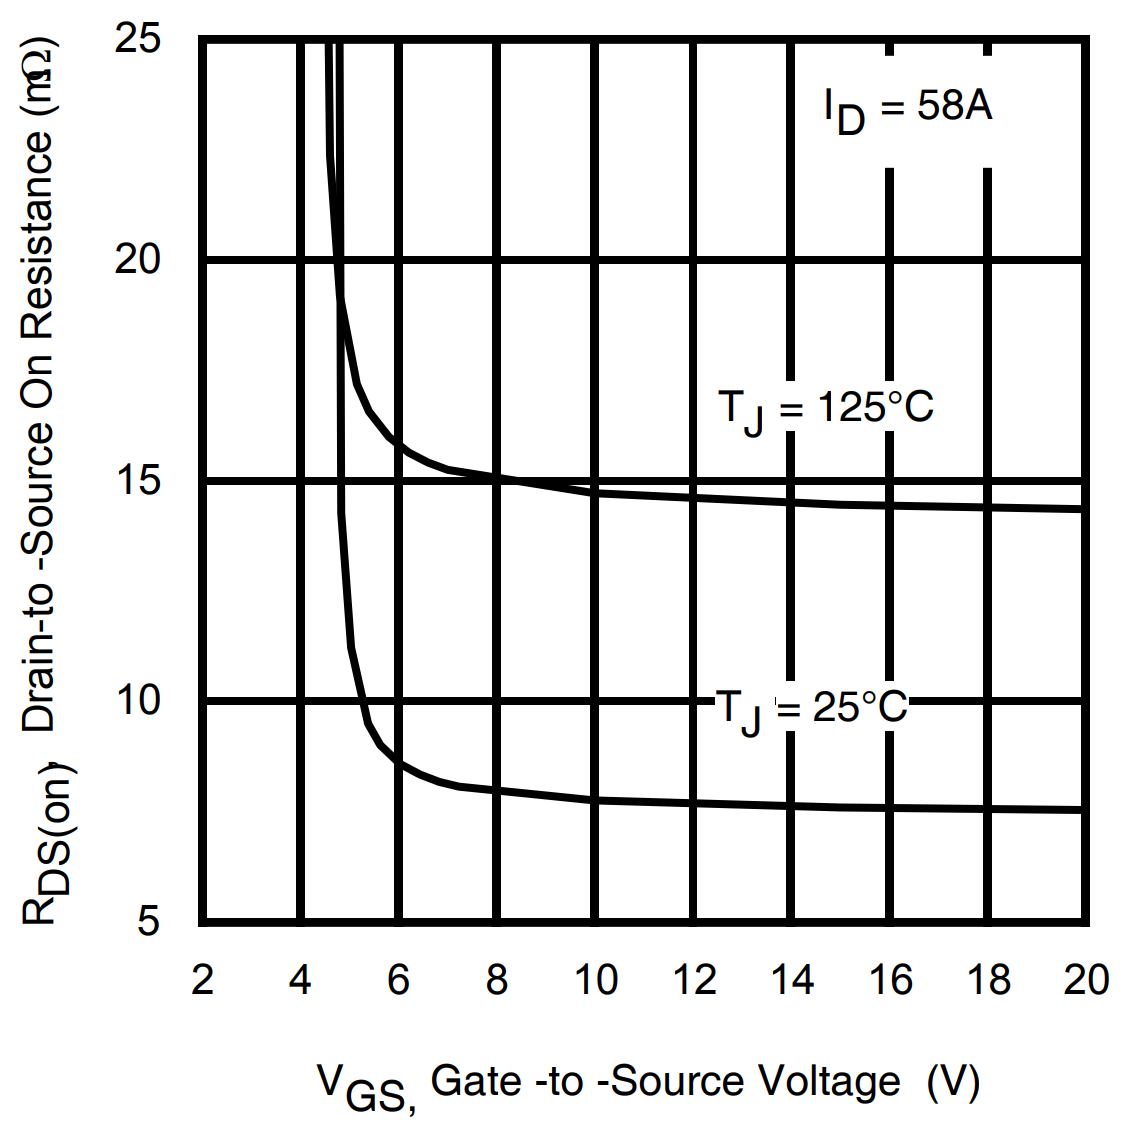
\includegraphics[width=0.6\linewidth]{graphics/mosfet_transfer_characteristic}
	\caption[Transfer characteristic of the IRF100B202.]{Transfer characteristic of the \texttt{IRF100B202} as per the datasheet.
	Inspecting the graph reveals that the maximum \id of 97A is reached at \vgs$\approx5.5\rightarrow6.5$V.}
	\label{fig:mosfettransfercharacteristic}
\end{figure}
 
Having chosen a MOSFET for the full-bridge, some form of driver must be designed for the full-bridge.
For this task, ready-made full-bridge drivers exist on the market that incorporate all of the electronics required to generate the driving signals, requiring only a PWM signal from the designer.
In order to choose one, a few parameters must be fulfilled.

\begin{itemize}
	\item \textbf{Output Current:} The amount of current necessary to properly drive the MOSFET.
	This value depends on the switching frequency of the application, the gate-to-source voltage ($V_{gs}$) and the total gate charge of the MOSFET.
	\item \textbf{Driving Voltage:} In order to ensure that the MOSFET is turned on quickly and fully the driver should be able to supply a voltage well above the gate threshold of the MOSFET.
	\item \textbf{High-Side Drive Capabilities:} The high side MOSFET of the full-bridge is referenced not to ground, but to a floating reference.
	This means that in order to switch on this MOSFET, $V_{\text{gate}}$ needs to be boosted compared to the floating reference. 
	This is bootstrapping and is explained in more detail in section \ref{ssub:bootstrap_circuit}.
	\item \textbf{Shoot-Through Protection and Deadtime:} Due to the structure of the full-bridge it is important that two MOSFETs on the same half-bridge are never \texttt{on} at the same time as this would result in a short from $V_{\text{cc}}$ to ground.
	This is resolved with a combination of deadtime (a delay where no MOSFET is \texttt{on}) and a logic table that ensures that an illegal switch combination can never happen.
\end{itemize}

The \texttt{HIP4081AIBZ} \cite{driver} full-bridge driver meets all of the above requirements.
It can supply up to 2.5A on the output pins with a voltage approximately 1V below \vcc, well above the required \vth.
It also allows for an external bootstrap circuit, which makes it able to drive the high-side MOSFETs.
Since the motor should, preferably, be driven outside the audible frequency range, it was chosen to set the switching frequency at 22kHz.
This frequency was chosen over an even higher frequency because increasing the frequency also increases the switching losses.
At this frequency there is $\frac{1}{22000}\approx45\mu$S per cycle. 
Well within this time the gate should be fully opened.
The switching time should be calculated to verify this.
\cite{mosfet_switch_app_note} describes switching characteristics of MOSFETs without taking parasitics into account.
Approximating the turn-on time of the MOSFET is sufficient here as it just needs to be verified that the MOSFETs are fully open within a small fraction of the switching period.
\cite{mosfet_switch_app_note} approximates the turn-on time of a MOSFET in equation \ref{eq:mosfet_turn_on}.

\begin{equation}
t_{switch} = R_G \cdot C_{iss} \cdot ln\left(\frac{1}{1-\frac{V_{gp}}{V_{GS}}}\right) 
\label{eq:mosfet_turn_on}
\end{equation}

Where $t_{switch}$ is the switching time, $R_G$ is the total gate resistance, $C_{iss}$ is the effective input capacitance of the
MOSFET, $V_{gp}$ is the gate plateau voltage and $V_{GS}$ is the voltage applied to the gate by the motor driver.
Accounting for voltage drops in the bootstrap circuit discussed later,  it is assumed that \vgs is 8V and by inspecting figure \ref{fig:mosfettransfercharacteristic}, $V_{gp}$ is estimated to 4.5V.
$R_G$ and $C_{iss}$ are   datasheet values.

\begin{equation}
t_{switch} = 9.4 \cdot 4.48 \cdot 10^{-9} \cdot ln\left(\frac{1}{1-\frac{4.5}{8}}\right) = 34.8 nS 
\label{eq:mosfet_turn_on_values}
\end{equation}
This MOSFET switching time is orders of magnitude smaller than the PWM switching period.

The component also has floating drive circuitry, meaning that by referencing the high-side driver to source of the high-side MOSFET, the driver can be made to output a voltage higher than \vcc.
This does require a few external components for bootstrapping.
The choice of these components and a more in depth explanation of the procedure is given in section \ref{ssub:bootstrap_circuit}.
Finally, the component has a user-programmable dead time and shoot-through protection. 

\subsubsection{Bootstrap Circuit}
\label{ssub:bootstrap_circuit}
\begin{figure}[h]
	\centering
	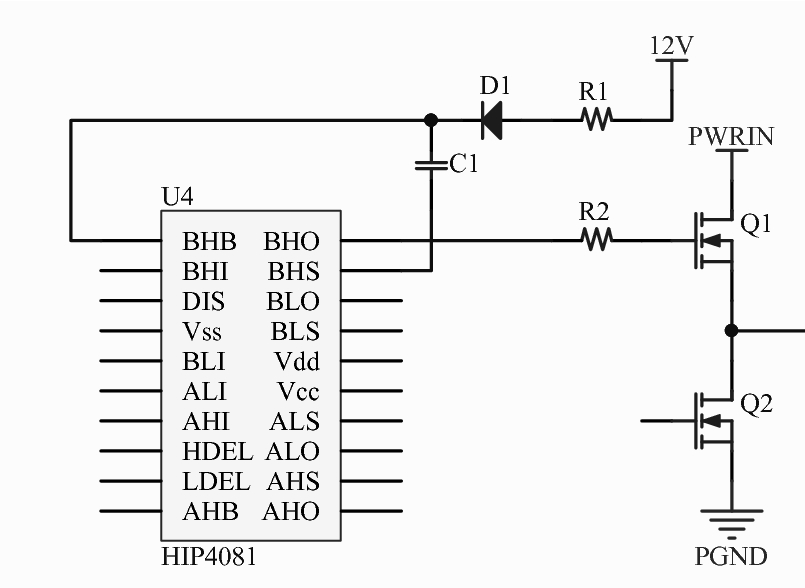
\includegraphics[width=0.6\linewidth]{graphics/hip_bootstrap}
	\caption[Bootstrap circuitry]{Bootstrap circuitry consisting of a diode, a capacitor and a resistor. }
	\label{fig:hip_bootstrap}
\end{figure}	
The chosen gate driver has floating drive circuitry for the high side MOSFETS but needs external bootstrap circuitry for providing the higher voltage. 
A standard bootstrap circuits consists of a diode, a capacitor and a resistor as shown in figure \ref{fig:hip_bootstrap}.
The advantage of using a bootstrap circuit to supply a high voltage for the floating drive is that it is very simple. 
The disadvantage is that it sets a limit for the maximum and minimum duty cycle as the bootstrap capacitor needs to be charged fully in each period.
The bootstrap circuitry for this project will be designed to have a maximum duty cycle for the higher MOSFETS of 95\%, thus meaning that the charging of the bootstrap capacitor should take no longer than 5\% of a period.  

The bootstrap diode needs to have a fast recovery time, preferably below 100 ns \cite{bootstrap_infineon}, to minimize the energy fed back to the supply from the bootstrap capacitor.
\texttt{US1M-E3} \cite{diode_ds} was chosen as it has a reverse recovery time of 75 ns and comes in SMD packaging. 
It allows for a maximum average forward current of 1 A and a maximum forward voltage drop of 1.7 V \cite{diode_ds}.
Determining the values for the bootstrap capacitor was done using the calculations shown in \cite{bootstrap_ON}.
The maximum allowed voltage drop across the bootstrap capacitor during \texttt{on} time needs to be determined: 
\begin{equation}
\Delta V_{boot} = V_{DD} - V_{F} - V_{GSMIN}
\end{equation}
Where $\Delta V_{boot}$ is the voltage drop across the bootstrap capacitor during \texttt{on} time, $V_{DD}$ is the supply voltage, $V_F$ is the forward voltage drop across the diode and $V_{GSMIN}$ is the minimum desired \texttt{gate-source} voltage.
$V_{GSMIN}$ was chosen to 8 V to to ensure a high enough gate voltage to turn on the MOSFETS. 
The chosen MOSFETS have a maximum gate threshold voltage of 3.5 V. 
Inserting the values yields the maximum allowed value of $\Delta V_{boot}$:
\begin{equation}
\Delta V_{boot} = 12 - 1.7 - 8 = 2.3 V	
\end{equation}

The total charge that needs to be supplied from the bootstrap capacitor is the gate charge of the MOSFET along with the quiescent and leakage currents in the \texttt{on} time:
\begin{equation}
	Q_{total} = Q_{gate} + Q_{ls} + (I_{lkgs} + I_{qbs} + I_{lk} + I_{lkd}) \cdot t_{on}
	\label{eq:charge_total}
\end{equation}
Where $Q_{gate}$ is the maximum total gate charge, $I_{lkgs}$ is the gate-source leakage current, $I_{qbs}$ is the gate driver quiescent current, $I_{lk}$ is the gate driver leakage current, $I_{lkd}$ is the diode leakage current, $ t_{on}$ is the \texttt{on} time and $Q_{ls}$ is the charge required by the internal level shifter in the gate driver.
\begin{table}[h]
\centering
\begin{tabular}{|l|l|l|l|l|l|l|}
 \hline
 $Q_{gate}$ 	& $Q_{ls}$ 	& $I_{lkgs}$ 	& $I_{qbs}$ 		& $I_{lk}$ 			& $I_{lkdiode}$ 	& $t_{on}$ 		\\ 	\hline
 $116$ [nC]		& $3$ [nC]	& $100$ [nA]	&$-30$ [$\mu$A]		& $1$ [$\mu$A]		& $1$ [nA]			& $43$ [$\mu$S]	\\ 	\hline
\end{tabular}
\caption[Parameter values used to determine total charge.]{Parameter values used in equation \ref{eq:charge_total}. $I_{qbs}$ and $I_{lk}$ are found in the gate driver data sheet. $Q_{ls}$ is set to 3nC for all high voltage gate drivers \cite{bootstrap_ON}. $I_{lkgs}$ and $Q_{gate}$ are MOSFET data sheet values and $I_{lkdiode}$  is a diode data sheet value. $t_{on}$ is calculated using 95\% dutycycle and 22kHz switching.}
\label{tab:bootstrap_parameter}
\end{table}
$t_{on}$ can be calculated knowing that the worst case duty cycle for the high side MOSFET is 95\% and the switching frequency is 22 kHz.
Inserting the values, shown in \ref{tab:bootstrap_parameter}, yields the minimum charge value of the capacitor:
\begin{equation}
	Q_{total} = 118 [nC]
\end{equation}

The minimum value of the bootstrap capacitor can now be calculated:
\begin{equation}
	C_{boot} = \frac{Q_{total}}{\Delta V_{boot}} = \frac{118}{2.3} = 51.2 [nF]
\end{equation}
A ceramic capacitor will be used as it has a negligible leakage current. 
Looking for SMD ceramic capacitors it was found that in the range of the found minimum value is 56, 68, 82 and 100 nF.
56 nF is, in theory, a big enough capacitor for the circuit, but a bigger capacitor is an advantage as $\Delta V_{boot}$ will then decrease.
When increasing the size of the capacitor it should be noted that the initial charge current will become larger.
It was therefore chosen to use a 100 nF ceramic capacitor.

The initial charge current to the capacitor needs to be limited in order not to exceed the maximum ratings of the diode.
Therefore a resistor is put in series with the diode.
The resistor value should not be too big as the voltage drop across it is subtracted from the bootstrap capacitor voltage.
A 4.7 $\Omega$ resistor was chosen. In this setting, the maximum current through this component is 2.6 A.
This is clearly above the maximum average forward current of the diode at 1A.
The diode can however, withstand an 8.3 ms single half sine-wave of maximum 30 A \cite{diode_ds}.
The capacitor voltage while charging in a RC circuit is described by equation \ref{eq:cap_charge}, according to \cite{prac_ele_for_inven}.

\begin{equation}
	V_C = V_S (1-e^{\frac{-t}{R\cdot C}})
	\label{eq:cap_charge}
\end{equation}

Where $V_C$ is the capacitor voltage, $V_S$ is the supply voltage, $R$ is the resistance and $C$ is the capacitance.
The RC time constant is defined as $\tau = R\cdot C$.
Equation \ref{eq:cap_charge} can be used to calculate the time it takes an RC circuit to charge to a specific level.
After one time constant the capacitor is charged 63.2\% and after five time constant the capacitor is approximately fully charged, 99.3\%.
This knowledge can be used to calculate the time it takes to initially charge the bootstrap capacitors as shown in equation \ref{eq:cap_boot_time}.

\begin{equation}
T_{charge,init} = 5\cdot \tau = 5\cdot (R \cdot C) = 5\cdot (4.7 \cdot 100 \cdot 10^{-9}) = 2.35 \mu S 
\label{eq:cap_boot_time}
\end{equation}

Meaning that the diode can be exposed to a maximum of 2.6A for $2.35 \mu S $, which is well below the absolute maximum rating.
It should also be noted that bootstrap capacitor needs at least $2.35 \mu S $ for the initial charging.

Lastly it should be calculated what the maximum allowed duty cycle for the high side MOSFETS are in this configuration, using the found components.
The time it takes to charge the capacitor the energy that is used in each period is:
\begin{equation}
	T_{charge,period} = 5\cdot (R \cdot C_{boot}) = 5\cdot (4.7 \cdot  51.6 \cdot 10^{-9}) = 1.21 \mu S 
\end{equation}
The $1.21 \mu S$ is equivalent to 2.7\% duty cycle and the maximum theoretical duty cycle for the high side MOSFETS is thus 97.3\%.
% subsection power_board (end)

\subsubsection{Supply Capacitors}
\label{ssub:sup_caps}
Driving an inductive load, such as a motor, requires capacitors placed close to the MOSFETS in order to minimize the voltage spikes created by the load current and parasitic inductance in the wires from the supply.
This section will determine the size and requirements of the supply capacitors using calculations and simulation in PLECS.

First off, the ripple current across the motor needs to be determined as this is the current the supply capacitors need to supply.
Equation \ref{eq:inductor_gen} shows the general inductor equation and in \ref{eq:inductor_rip} it is refactored to calculate the ripple current.
\begin{equation}
	V(t) = L \cdot \frac{dI(t)}{dt}
	\label{eq:inductor_gen}
\end{equation}

\begin{equation}
	\Delta I = \frac{\Delta V}{L} \Delta t
	\label{eq:inductor_rip}
\end{equation}

The highest ripple current is found when the duty cycle is 50$\%$ and the full voltage of 24V is applied as calculated in equation \ref{eq:inductor_rip_size}.

\begin{equation}
	\Delta I = \frac{24}{82\cdot 10^{-6}} \cdot 0.5 \cdot \frac{1}{22000} = 6.7 [A] 
	\label{eq:inductor_rip_size}
\end{equation}

The peak-to-peak ripple current of $6.7$A is also found when simulating the system using PLECS as shown in figure \ref{fig:sim_currents}.
The load current experienced by the supply is also shown in figure \ref{fig:sim_currents}, where abrupt changes in current are seen. 

\begin{figure}[h]
	\centering
	%% This file was created by matlab2tikz.
%
%The latest updates can be retrieved from
%  http://www.mathworks.com/matlabcentral/fileexchange/22022-matlab2tikz-matlab2tikz
%where you can also make suggestions and rate matlab2tikz.
%
\definecolor{mycolor1}{rgb}{0.00000,0.44700,0.74100}%
%
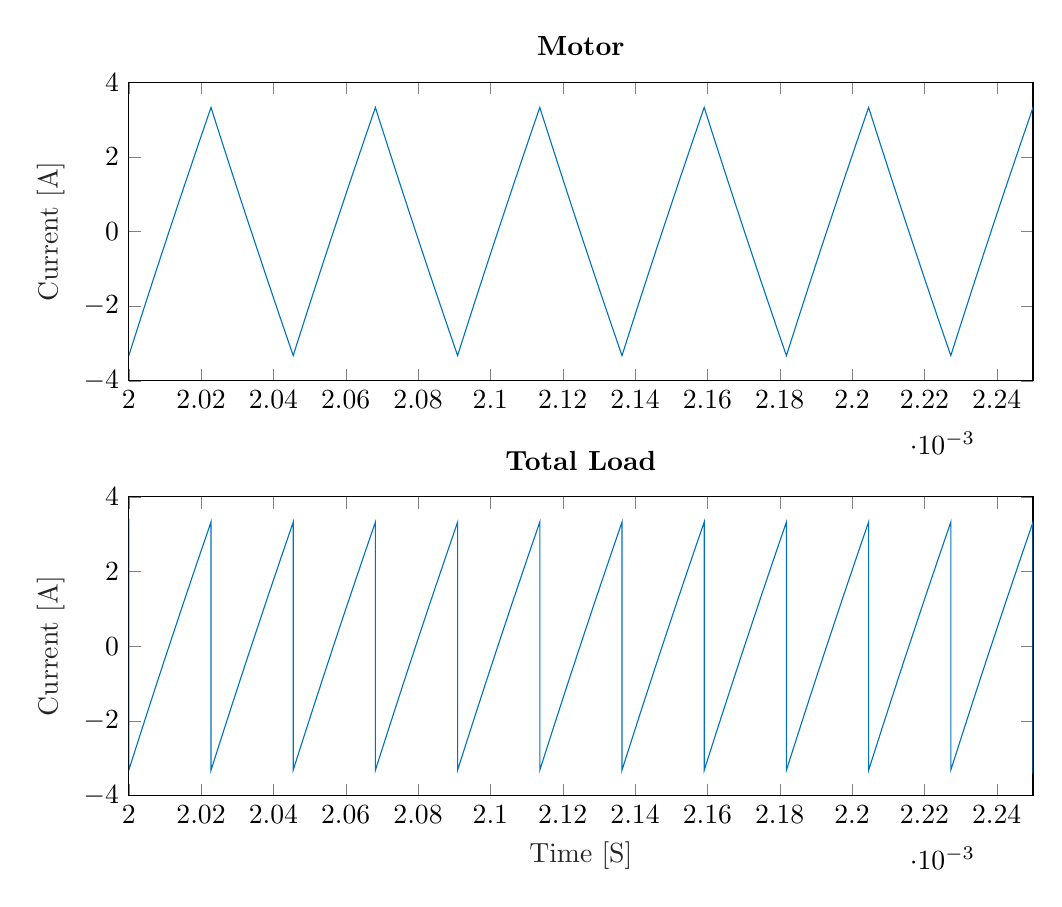
\begin{tikzpicture}

\begin{axis}[%
width=4.521in,
height=1.493in,
at={(0.758in,2.554in)},
scale only axis,
xmin=0.002,
xmax=0.00225,
ymin=-4,
ymax=4,
ylabel style={font=\color{white!15!black}},
ylabel={Current [A]},
axis background/.style={fill=white},
title style={font=\bfseries},
title={Motor}
]
\addplot [color=mycolor1, forget plot]
  table[row sep=crcr]{%
0	0\\
3.3460025901564e-08	0.00979216834185557\\
6.6920051803128e-08	0.0195831689424556\\
1.00380077704692e-07	0.0293729772080969\\
2.86236444194498e-07	0.0837307082176497\\
4.72092810684304e-07	0.138052159786677\\
6.5794917717411e-07	0.192336888519681\\
8.43805543663915e-07	0.2465847436031\\
1.46206269418065e-06	0.426776921334415\\
2.08031984469738e-06	0.606560789436667\\
2.69857699521411e-06	0.785936710694134\\
3.31683414573084e-06	0.964905205652303\\
3.93509129624758e-06	1.1434666409016\\
5.75197157684523e-06	1.6658548409378\\
7.56885185744287e-06	2.18473747278615\\
9.38573213804052e-06	2.70012165466927\\
1.12026124186382e-05	3.21201571005084\\
1.30194926992358e-05	3.72042845969404\\
1.48363729798335e-05	4.22536872362558\\
1.97586180405918e-05	5.57596587927003\\
2.27272727272725e-05	6.3783171170272\\
2.27272727272727e-05	6.37831711702726\\
2.27410076969546e-05	6.37398638046111\\
2.27547426666364e-05	6.36965375955969\\
2.27684776363182e-05	6.36532285013984\\
2.29058273331366e-05	6.32203472687713\\
2.30431770299549e-05	6.27876729316781\\
2.31805267267732e-05	6.2355202943356\\
2.44483529688856e-05	5.83725566814237\\
2.57161792109979e-05	5.44072022747552\\
2.69840054531102e-05	5.04592126779853\\
2.82518316952226e-05	4.65286095881394\\
3.11224300272083e-05	3.76931165867921\\
3.3993028359194e-05	2.89464378808499\\
3.68636266911797e-05	2.02882734038762\\
3.97342250231655e-05	1.17183245052039\\
4.26048233551512e-05	0.323631784651184\\
4.5454545454545e-05	-0.509728483636083\\
4.54545454545455e-05	-0.509728483636209\\
4.56137030196537e-05	-0.462855930246644\\
4.5772860584762e-05	-0.416009673465522\\
4.59320181498702e-05	-0.369190286586476\\
4.75235938009527e-05	0.096688919165212\\
4.91151694520353e-05	0.559938654993594\\
5.07067451031178e-05	1.02051267646793\\
5.21877413094701e-05	1.44673915057175\\
5.36687375158223e-05	1.87064481037127\\
5.48032708460027e-05	2.19395845751998\\
5.59378041761831e-05	2.51590586535985\\
5.70723375063635e-05	2.83649721774212\\
5.90623960561229e-05	3.39602028595376\\
6.10524546058824e-05	3.95161284857696\\
6.30425131556419e-05	4.50312800819581\\
6.50325717054013e-05	5.05052048240398\\
6.81818181818173e-05	5.9083681446256\\
6.81818181818182e-05	5.90836814462583\\
6.81982265228205e-05	5.90321766823039\\
6.82146348638228e-05	5.8980650799626\\
6.82310432048251e-05	5.8929146034375\\
6.83951266148483e-05	5.8414383259708\\
6.85592100248715e-05	5.78999120622817\\
6.87232934348947e-05	5.73857317088326\\
7.03641275351264e-05	5.22594260544655\\
7.20049616353581e-05	4.71619997502048\\
7.36457957355898e-05	4.20935629332506\\
7.52866298358215e-05	3.70541426066593\\
7.86734614243063e-05	2.67439183644975\\
8.2060293012791e-05	1.65568679003902\\
8.54471246012758e-05	0.649258995332076\\
8.88339561897606e-05	-0.344931641381534\\
9.090909090909e-05	-0.948049426664154\\
9.09090909090909e-05	-0.948049426664405\\
9.10680548465105e-05	-0.900944972184585\\
9.12270187839301e-05	-0.85386684032189\\
9.13859827213497e-05	-0.806815624783133\\
9.28881448030836e-05	-0.364268712879095\\
9.43903068848175e-05	0.075924523168433\\
9.58924689665514e-05	0.513722225414341\\
9.73937786098869e-05	0.948873891503222\\
9.88950882532224e-05	1.38163182114456\\
0.000100396397896558	1.81199872685562\\
0.000102388285618672	2.37990759343637\\
0.000104380173340787	2.94391803819557\\
0.000106372061062901	3.50382863193594\\
0.000108363948785016	4.0595734864279\\
0.000112581062122341	5.22245152431999\\
0.000113636363636363	5.51053783719038\\
0.000113636363636364	5.51053783719062\\
0.000113652875841073	5.50537508343307\\
0.000113669388045783	5.50021036711542\\
0.000113685900250493	5.49504766058541\\
0.000113851022297591	5.44344929732303\\
0.000114016144344688	5.39188054216774\\
0.000114181266391786	5.3403413740717\\
0.000115832486862763	4.82652639019902\\
0.00011748370733374	4.31564953083607\\
0.000119134927804716	3.80772280116105\\
0.000120786148275693	3.3027493167972\\
0.000124260197469801	2.24994846748255\\
0.000127734246663909	1.21017549199153\\
0.000131208295858018	0.183388685607617\\
0.000134682345052126	-0.830455009606617\\
0.000136363636363635	-1.31647681541512\\
0.000136363636363636	-1.31647681541562\\
0.000136457648355821	-1.28848834726951\\
0.000136551660348006	-1.26050912560564\\
0.000136645672340192	-1.2325394005705\\
0.000137585792262042	-0.953660414443846\\
0.000138525912183893	-0.675711762263763\\
0.000139466032105744	-0.398710450483822\\
0.000141080921833001	0.0744903471438776\\
0.000142695811560257	0.544923535047713\\
0.00014397637111121	0.916137663936403\\
0.000145256930662163	1.2855871880448\\
0.000146309638560935	1.58807403635747\\
0.000147362346459708	1.88937169227974\\
0.00014841505435848	2.18948675148099\\
0.000150446951617213	2.76585105914289\\
0.000152478848875945	3.33804096395515\\
0.000154510746134677	3.90591581582167\\
0.000156542643393409	4.4694327063089\\
0.000159090909090907	5.17002081333405\\
0.000159090909090909	5.17002081333453\\
0.000159107950404141	5.16471547697748\\
0.000159124991717373	5.15940825618861\\
0.000159142033030604	5.15410303483625\\
0.000159312446162921	5.10108115055827\\
0.000159482859295238	5.0480908629433\\
0.000159653272427556	4.99513222149086\\
0.000161357403750727	4.46723180551256\\
0.000163061535073897	3.94247263127644\\
0.000164765666397068	3.4208672561975\\
0.000166469797720239	2.90241812883423\\
0.000170111015763006	1.80520238710783\\
0.000173752233805772	0.722332913291956\\
0.000177393451848539	-0.346247160573399\\
0.000181034669891305	-1.40059735141266\\
0.00018181818181818	-1.62561618975527\\
0.000181818181818182	-1.62561618975576\\
0.00018189191245417	-1.60360142523706\\
0.000181965643090158	-1.58159233486036\\
0.000182039373726146	-1.55958910529188\\
0.000182776680086025	-1.34006159444278\\
0.000183513986445904	-1.1211080471627\\
0.000184251292805783	-0.902738959943471\\
0.000186176642929505	-0.336111723359008\\
0.000188101993053228	0.226593340319752\\
0.000189433381211277	0.61367738328916\\
0.000190764769369326	0.998843310781422\\
0.000191862820760937	1.31517016011703\\
0.000192960872152549	1.63020214326219\\
0.000194058923544161	1.94394679035387\\
0.000196139234286316	2.53528966757863\\
0.000198219545028471	3.1222613516525\\
0.000200299855770626	3.70471321364354\\
0.000202380166512781	4.28260111282239\\
0.000204545454545453	4.87927070065436\\
0.000204545454545455	4.87927070065483\\
0.000204563248495638	4.87375397959641\\
0.000204581042445821	4.86823541514357\\
0.000204598836396004	4.86271888414652\\
0.000204776775897834	4.80758616239875\\
0.000204954715399664	4.75248770523977\\
0.000205132654901494	4.69742363897177\\
0.000206912049919797	4.14861455983025\\
0.0002086914449381	3.60321712392594\\
0.000210470839956403	3.06124426527418\\
0.000212250234974706	2.52269735314441\\
0.000215992339235271	1.40127193130843\\
0.000219734443495837	0.294915233950511\\
0.000223476547756402	-0.796443118277702\\
0.000227218652016968	-1.87287598395711\\
0.000227272727272726	-1.88832192980601\\
0.000227272727272727	-1.8883219298065\\
0.000227342297857368	-1.8674965214086\\
0.000227411868442008	-1.8466761249662\\
0.000227481439026648	-1.82586092362373\\
0.000228177144873052	-1.61815622510643\\
0.000228872850719455	-1.41096013261674\\
0.000229568556565858	-1.20428192867981\\
0.000231740906602734	-0.561959842495436\\
0.00023391325663961	0.0754652928433671\\
0.000236085606676486	0.707897523625743\\
0.000238257956713362	1.33531177211176\\
0.000242602494028023	2.57508628531837\\
0.000246947031342683	3.79491169755634\\
0.000249999999999997	4.6402370224219\\
0.00025	4.64023702242285\\
0.000250019628217504	4.63416863641626\\
0.000250039256435008	4.62809832974944\\
0.000250058884652512	4.6220302822174\\
0.000250255166827551	4.56138855762422\\
0.00025045144900259	4.50078810165967\\
0.00025064773117763	4.44022919509232\\
0.000252610552928023	3.83685231936177\\
0.000254573374678417	3.23759512538674\\
0.000256536196428811	2.64247348184285\\
0.000258499018179204	2.05148839219246\\
0.00026230269607791	0.917985886864917\\
0.000266106373976615	-0.200068898448616\\
0.000269910051875321	-1.30274624539011\\
0.000272727272727269	-2.10958190663542\\
0.000272727272727273	-2.10958190663641\\
0.000272768691766965	-2.0971445132162\\
0.000272810110806658	-2.08470883916461\\
0.00027285152984635	-2.0722750015498\\
0.000273265720243275	-1.9480945773949\\
0.000273679910640201	-1.82409380817647\\
0.000274094101037126	-1.7002760300248\\
0.000276474575282944	-0.99201519218526\\
0.000278855049528763	-0.289700777080019\\
0.000281235523774581	0.406610503044831\\
0.0002836159980204	1.09690909829915\\
0.000287927361167765	2.3318709333071\\
0.00029223872431513	3.54723458490537\\
0.000295454545454542	4.44107226812169\\
0.000295454545454545	4.44107226812265\\
0.000295475547795918	4.43458904568205\\
0.00029549655013729	4.42810387748598\\
0.000295517552478663	4.42162112001525\\
0.000295727575892386	4.35683736126698\\
0.00029593759930611	4.29210065463151\\
0.000296147622719834	4.22741141574417\\
0.00029824785685707	3.58304649672565\\
0.000300348090994307	2.94338836213575\\
0.000302448325131544	2.30845678951722\\
0.000304548559268781	1.67825391184348\\
0.00030840178706574	0.534311601515325\\
0.0003122550148627	-0.593790092823967\\
0.00031610824265966	-1.70611431376052\\
0.000318181818181815	-2.29819353211022\\
0.000318181818181818	-2.29819353211121\\
0.000318216910128822	-2.28762391738447\\
0.000318252002075825	-2.27705551476598\\
0.000318287094022829	-2.26648843514806\\
0.000318638013492865	-2.16093137669381\\
0.000318988932962902	-2.05550369377823\\
0.000319339852432938	-1.9502078029123\\
0.000321730696804805	-1.23616395699821\\
0.000324121541176672	-0.528156744987434\\
0.000326512385548539	0.173765399113965\\
0.000328903229920406	0.86959462059652\\
0.00033321923055222	2.11033039144202\\
0.000337535231184035	3.33132093693318\\
0.000340909090909087	4.27209444587003\\
0.000340909090909091	4.27209444587099\\
0.000340929953026185	4.26566360640344\\
0.000340950815143279	4.25923092687039\\
0.000340971677260373	4.25280056340677\\
0.000341180298431315	4.18854027505537\\
0.000341388919602256	4.12432661772937\\
0.000341597540773198	4.06016002069595\\
0.000343683752482612	3.42100022909339\\
0.000345769964192026	2.78650799915323\\
0.00034785617590144	2.15670388491997\\
0.000349942387610854	1.53159074565621\\
0.000353862201477184	0.369717249245569\\
0.000357782015343514	-0.775670764458827\\
0.000361701829209844	-1.90463829879655\\
0.00036363636363636	-2.4557839306292\\
0.000363636363636364	-2.45578393063018\\
0.000363695905167082	-2.43781680581856\\
0.0003637554466978	-2.41985333442861\\
0.000363814988228518	-2.40189369272165\\
0.000364410403535697	-2.22262684696784\\
0.000365005818842876	-2.04373481884366\\
0.000365601234150056	-1.86522453974338\\
0.000367733905497417	-1.22871314865743\\
0.000369866576844778	-0.596973919648128\\
0.00037199924819214	0.0299106828227297\\
0.000374131919539501	0.651918245296275\\
0.000378286707189542	1.84971523249257\\
0.000382441494839584	3.02908508269167\\
0.000386363636363633	4.12559464964425\\
0.000386363636363636	4.12559464964521\\
0.000386384269576468	4.11924763877802\\
0.0003864049027893	4.11289888699914\\
0.000386425536002132	4.10655235313425\\
0.00038663186813045	4.04312954041196\\
0.000386838200258768	3.97975253166327\\
0.000387044532387087	3.9164217548111\\
0.000389107853670269	3.28557577049391\\
0.000391171174953452	2.65931428327555\\
0.000393234496236635	2.03765657969553\\
0.000395297817519818	1.42060435284609\\
0.000399334545479002	0.226675050717639\\
0.000403371273438187	-0.949722711864358\\
0.000407408001397371	-2.10867110538955\\
0.000409090909090906	-2.58670278815743\\
0.000409090909090909	-2.58670278815841\\
0.000409145988200711	-2.57006869975492\\
0.000409201067310513	-2.55343772732207\\
0.000409256146420314	-2.53681004004178\\
0.000409806937518332	-2.37081577150612\\
0.00041035772861635	-2.20514289195094\\
0.000410908519714368	-2.03979732611326\\
0.000413097374837221	-1.38570589615075\\
0.000415286229960075	-0.736662299855921\\
0.000417475085082928	-0.0927420918712096\\
0.000419663940205782	0.546036608826598\\
0.000423968638727064	1.78733142560619\\
0.000428273337248345	3.00885908076593\\
0.000431818181818178	4.00000969233672\\
0.000431818181818182	4.00000969233768\\
0.000431839275076628	3.99353552660101\\
0.000431860368335074	3.98705965072965\\
0.00043188146159352	3.98058601084854\\
0.000432092394177982	3.91589377431785\\
0.000432303326762444	3.85124925285408\\
0.000432514259346906	3.78665292130374\\
0.000434623585191524	3.14325497709778\\
0.000436732911036143	2.50463347912925\\
0.000438842236880761	1.87080710832231\\
0.000440951562725379	1.24177588616619\\
0.000445050033039373	0.033222969508128\\
0.000449148503353368	-1.15734363531676\\
0.000453246973667362	-2.33001970722991\\
0.000454545454545451	-2.69783234439024\\
0.000454545454545455	-2.69783234439122\\
0.0004546010289307	-2.6810357358428\\
0.000454656603315945	-2.66424228174699\\
0.00045471217770119	-2.64745215665824\\
0.000455267921553643	-2.47983724349932\\
0.000455823665406095	-2.31254794770271\\
0.000456379409258548	-2.14559025346581\\
0.00045868446959878	-1.45638550216304\\
0.000460989529939011	-0.772755065198986\\
0.000463294590279243	-0.0947766643127222\\
0.000465599650619475	0.577532800723047\\
0.000469812892476408	1.79178792665153\\
0.00047402613433334	2.98722540848639\\
0.000477272727272724	3.89562762531595\\
0.000477272727272727	3.89562762531692\\
0.000477295402708081	3.88867685276398\\
0.000477318078143435	3.88172431169523\\
0.000477340753578789	3.87477420698354\\
0.00047756750793233	3.80532349876055\\
0.00047779426228587	3.73592750259582\\
0.000478021016639411	3.66658683909998\\
0.000480288560174816	2.97612537432033\\
0.000482556103710221	2.2911466103743\\
0.000484823647245627	1.61167189153912\\
0.000487091190781032	0.937700586480311\\
0.0004911972102979	-0.268747565625874\\
0.000495303229814769	-1.45726632153262\\
0.000499409249331637	-2.62794765330139\\
0.000499999999999993	-2.79491648591443\\
0.0005	-2.79491648591639\\
0.000500056745332312	-2.77773991812249\\
0.000500113490664625	-2.76056662433982\\
0.000500170235996937	-2.7433967858544\\
0.000500737689320059	-2.57199560250605\\
0.000501305142643181	-2.40093240187529\\
0.000501872595966304	-2.23021341017497\\
0.0005042220697522	-1.52677175839865\\
0.000506571543538096	-0.82909706902467\\
0.000508921017323993	-0.13727111682226\\
0.000511270491109889	0.548687186320934\\
0.000515312721773524	1.71516833038822\\
0.000519354952437159	2.86437520456513\\
0.000522727272727266	3.80997447787648\\
0.000522727272727273	3.80997447787841\\
0.000522751306376193	3.80260956304194\\
0.000522775340025112	3.79524284019986\\
0.000522799373674032	3.78787872694102\\
0.00052303971016323	3.71429372360279\\
0.000523280046652429	3.64076999567818\\
0.000523520383141627	3.5673083060386\\
0.000525923748033608	2.83599396327517\\
0.000528327112925589	2.11082782882618\\
0.00053073047781757	1.39183576438828\\
0.000533133842709552	0.679018548237901\\
0.000537260952310566	-0.530676430903125\\
0.000541388061911581	-1.72226439533256\\
0.000545454545454538	-2.87871812611635\\
0.000545454545454545	-2.87871812611831\\
0.000545486180018228	-2.86912514916799\\
0.000545517814581911	-2.8595331259129\\
0.000545549449145593	-2.84994218099589\\
0.00054586579478242	-2.75412535242025\\
0.000546182140419247	-2.6584138746077\\
0.000546498486056073	-2.56280971682326\\
0.000549178672768715	-1.75696300434028\\
0.000551858859481356	-0.958736172524893\\
0.000554539046193997	-0.168173259747465\\
0.000557219232906638	0.614723414826821\\
0.000561655004217416	1.89363760386096\\
0.000566090775528194	3.15168366267871\\
0.000568181818181811	3.73752534370516\\
0.000568181818181818	3.7375253437071\\
0.000568204374702	3.73061523223814\\
0.000568226931222183	3.72370345512032\\
0.000568249487742365	3.71679402093937\\
0.000568475052944188	3.64774953282531\\
0.00056870061814601	3.5787593104649\\
0.000568926183347833	3.50982399161644\\
0.000571181835366059	2.82339433550953\\
0.000573437487384285	2.14240849124595\\
0.000575693139402512	1.46689070606884\\
0.000577948791420738	0.796843322804897\\
0.000582052143327392	-0.408073274081108\\
0.000586155495234045	-1.59497825135928\\
0.000590258847140698	-2.76394951597553\\
0.000590909090909084	-2.94755175578491\\
0.000590909090909091	-2.94755175578686\\
0.000590959516508872	-2.93224744789989\\
0.000591009942108653	-2.91694572218636\\
0.000591060367708434	-2.9016467496346\\
0.000591564623706245	-2.74889373863545\\
0.000592068879704056	-2.59640995633824\\
0.000592573135701867	-2.44420039697188\\
0.000594806470108126	-1.77314317467297\\
0.000597039804514385	-1.10735382280102\\
0.000599273138920644	-0.446903358238594\\
0.000601506473326903	0.208190915834121\\
0.00060562356989688	1.40183446476566\\
0.000609740666466858	2.57736402826412\\
0.000613636363636357	3.67308133027466\\
0.000613636363636364	3.6730813302766\\
0.000613658997831899	3.66615504921932\\
0.000613681632027435	3.659227138088\\
0.000613704266222971	3.65230155337451\\
0.000613930608178328	3.58309606308871\\
0.000614156950133686	3.51394544866726\\
0.000614383292089044	3.44485036449075\\
0.000616646711642621	2.75685598957649\\
0.000618910131196197	2.07436620421114\\
0.000621173550749774	1.39740429101896\\
0.000623436970303351	0.725971107171847\\
0.000627677556364823	-0.517138145095901\\
0.000631918142426295	-1.74095778077408\\
0.000636158728487766	-2.9455859564701\\
0.000636363636363629	-3.00331014568189\\
0.000636363636363636	-3.00331014568384\\
0.000636411774985549	-2.98870023000527\\
0.000636459913607462	-2.97409266156562\\
0.000636508052229375	-2.95948760777894\\
0.000636989438448505	-2.81365322086834\\
0.000637470824667636	-2.66806466279908\\
0.000637952210886766	-2.52272648006007\\
0.000640230433047751	-1.83807381280985\\
0.000642508655208737	-1.15891824123425\\
0.000644786877369722	-0.485326301282013\\
0.000647065099530707	0.182688139322527\\
0.000651328090495629	1.41773140438894\\
0.000655591081460551	2.63336676503023\\
0.000659090909090902	3.61695067654711\\
0.000659090909090909	3.61695067654904\\
0.000659113697178817	3.6099869464973\\
0.000659136485266725	3.60302160918081\\
0.000659159273354632	3.59605859352666\\
0.000659387154233711	3.52647932037585\\
0.000659615035112789	3.45695555136827\\
0.000659842915991867	3.38748795497388\\
0.00066212172478265	2.69580194660462\\
0.000664400533573433	2.00968193233982\\
0.000666679342364216	1.32914969923046\\
0.000668958151154999	0.654204206966739\\
0.000673235101280136	-0.597522967597643\\
0.000677512051405274	-1.82970762167744\\
0.000681789001530411	-3.0424607158537\\
0.000681818181818175	-3.05066848260151\\
0.000681818181818182	-3.05066848260346\\
0.000681867400727158	-3.03573029319104\\
0.000681916619636135	-3.02079454896102\\
0.000681965838545111	-3.00586142163829\\
0.000682458027634877	-2.85675508088465\\
0.000682950216724642	-2.70790454309517\\
0.000683442405814408	-2.5593145250162\\
0.00068584486093225	-1.83752792427101\\
0.000688247316050092	-1.12182718836945\\
0.000690649771167934	-0.412281384830144\\
0.000693052226285776	0.291097022064598\\
0.000697289964889382	1.51681154233223\\
0.000701527703492988	2.72346631983952\\
0.000704545454545448	3.57118536592226\\
0.000704545454545455	3.5711853659242\\
0.000704569606390293	3.56380966426512\\
0.000704593758235132	3.55643230005062\\
0.00070461791007997	3.54905743974744\\
0.000704859428528357	3.47536540280112\\
0.000705100946976743	3.40173529149833\\
0.000705342465425129	3.3281679038408\\
0.000707757649908989	2.59583229088773\\
0.00071017283439285	1.86971022719993\\
0.000712588018876711	1.14982575254601\\
0.000715003203360571	0.43617706654896\\
0.000719259333388766	-0.806311727672883\\
0.00072351546341696	-2.02956844908724\\
0.00072727272727272	-3.09354666523168\\
0.000727272727272727	-3.09354666523363\\
0.000727301820660392	-3.08470881389707\\
0.000727330914048057	-3.07587174739178\\
0.000727360007435721	-3.0670355924061\\
0.000727650941312369	-2.97875231388577\\
0.000727941875189016	-2.89055805839654\\
0.000728232809065664	-2.80245448740684\\
0.000731142147832138	-1.92624410168509\\
0.000734051486598613	-1.05901259923018\\
0.000736960825365087	-0.200795324876609\\
0.000739335092513641	0.492905872608331\\
0.000741709359662195	1.18062059080546\\
0.000744083626810749	1.86236520045248\\
0.000746457893959304	2.5381564815441\\
0.000749999999999993	3.53532238998109\\
0.00075	3.53532238998303\\
0.000750025853381898	3.52742525753135\\
0.000750051706763797	3.51952639194461\\
0.000750077560145695	3.51163027409671\\
0.000750336093964679	3.43273347847176\\
0.000750594627783664	3.35390743438593\\
0.000750853161602648	3.27515312273811\\
0.000753438499792491	2.49142822359744\\
0.000756023837982335	1.71481032298366\\
0.000758609176172178	0.945328859431727\\
0.000761194514362021	0.182983260500955\\
0.000765477800099492	-1.06437882362051\\
0.000769761085836963	-2.29227341390428\\
0.000772727272727266	-3.13123516630411\\
0.000772727272727273	-3.13123516630606\\
0.000772754977390944	-3.1228093715132\\
0.000772782682054615	-3.11438427974988\\
0.000772810386718286	-3.10596001596886\\
0.000773087433354995	-3.02178848617128\\
0.000773364479991704	-2.93769783381988\\
0.000773641526628413	-2.85368957260713\\
0.000776411992995503	-2.01799250891406\\
0.000779182459362593	-1.19045816110366\\
0.000781952925729684	-0.371122885944089\\
0.000784723392096774	0.440015235718401\\
0.000789202030097114	1.73398461291325\\
0.000793680668097454	3.00667141840257\\
0.000795454545454538	3.50489101477496\\
0.000795454545454545	3.5048910147769\\
0.000795478108210399	3.49769234966097\\
0.000795501670966254	3.49049209829456\\
0.000795525233722108	3.48329422818896\\
0.000795760861280649	3.41136954037456\\
0.00079599648883919	3.33950394578322\\
0.000796232116397731	3.26769820325311\\
0.000798588391983141	2.55282762142207\\
0.000800944667568551	1.84389055190394\\
0.000803300943153962	1.14091336619295\\
0.000805657218739372	0.443897937344929\\
0.000809860504460401	-0.784718776574724\\
0.00081406379018143	-1.99446583025146\\
0.000818181818181811	-3.16145818115488\\
0.000818181818181818	-3.16145818115683\\
0.000818208304958443	-3.15339890850446\\
0.000818234791735068	-3.14534027352761\\
0.000818261278511692	-3.13728239956589\\
0.00081852614627794	-3.05676902986694\\
0.000818791014044187	-2.9763300100322\\
0.000819055881810434	-2.89596673234053\\
0.000821704559472908	-2.0963658637716\\
0.000824353237135381	-1.30426982789083\\
0.000827001914797854	-0.519712629203635\\
0.000829650592460327	0.257307038474952\\
0.000834174963370509	1.5671987597602\\
0.000838699334280692	2.85524382005248\\
0.000840909090909084	3.47643510945626\\
0.000840909090909091	3.4764351094582\\
0.000840954677792677	3.46251758155155\\
0.000841000264676263	3.44859777574353\\
0.000841045851559849	3.43468422612319\\
0.000841501720395709	3.2957459094875\\
0.000841957589231569	3.15702840378899\\
0.000842413458067428	3.01853575137297\\
0.000844769996074047	2.30599583304009\\
0.000847126534080666	1.59935691324165\\
0.000849483072087285	0.898683946083332\\
0.000851839610093904	0.203990354457736\\
0.000856020070791418	-1.0137113550552\\
0.000860200531488933	-2.21270182900457\\
0.000863636363636357	-3.18418775971003\\
0.000863636363636364	-3.18418775971198\\
0.000863686098656619	-3.16906109162143\\
0.000863735833676874	-3.15393693052189\\
0.000863785568697129	-3.13881545490905\\
0.00086428291889968	-2.98783151523936\\
0.000864780269102232	-2.83711007901994\\
0.000865277619304783	-2.68665599740934\\
0.000867573450500194	-1.99537988365695\\
0.000869869281695606	-1.30968523939607\\
0.000872165112891018	-0.629641628496178\\
0.000874460944086429	0.0447361555687209\\
0.000878671764599989	1.26693808418357\\
0.000882882585113549	2.47019537232537\\
0.000886363636363629	3.45069098623202\\
0.000886363636363636	3.45069098623396\\
0.000886387277459498	3.44348024511563\\
0.00088641091855536	3.43626794885928\\
0.000886434559651223	3.42905801979278\\
0.000886670970609843	3.35701320477868\\
0.000886907381568464	3.28502804296674\\
0.000887143792527084	3.213103302776\\
0.00088950790211329	2.49707187988307\\
0.000891872011699495	1.78702674859826\\
0.0008942361212857	1.08299130680381\\
0.000896600230871906	0.38496391142884\\
0.000900963332813397	-0.887561551892704\\
0.000905326434754887	-2.13976998015356\\
0.000909090909090902	-3.20393661994027\\
0.000909090909090909	-3.20393661994222\\
0.000909116871259165	-3.19604207791431\\
0.000909142833427421	-3.18814814185111\\
0.000909168795595677	-3.18025493529746\\
0.000909428417278235	-3.10138553390766\\
0.000909688038960794	-3.02258740020495\\
0.000909947660643352	-2.94386186469346\\
0.000912543877468937	-2.1604697147955\\
0.000915140094294522	-1.38426648770981\\
0.000917736311120107	-0.615281077270572\\
0.000920332527945692	0.146491511062605\\
0.000924846675869267	1.45390325676827\\
0.000929360823792843	2.73968364980096\\
0.000931818181818175	3.43057643354851\\
0.000931818181818182	3.43057643355045\\
0.000931842710776115	3.42309763681912\\
0.000931867239734048	3.4156172473726\\
0.000931891768691982	3.40813934462089\\
0.000932137058271314	3.3334184954259\\
0.000932382347850647	3.25876147977272\\
0.000932627637429979	3.18416914939987\\
0.000935080533223305	2.44168848543255\\
0.000937533429016631	1.7056154187625\\
0.000939986324809956	0.975974767006524\\
0.000942439220603282	0.252764397766593\\
0.000946748269809004	-1.00219212747075\\
0.000951057319014726	-2.23744364592525\\
0.000954545454545448	-3.22301209394275\\
0.000954545454545455	-3.2230120939447\\
0.000954572995511052	-3.21463318958813\\
0.000954600536476649	-3.20625497500763\\
0.000954628077442246	-3.19787757792945\\
0.000954903487098218	-3.11417380509729\\
0.000955178896754189	-3.03054987088723\\
0.00095545430641016	-2.94700726629682\\
0.000958208402969875	-2.11590918022893\\
0.00096096249952959	-1.29286509595113\\
0.000963716596089305	-0.477907926216133\\
0.00096647069264902	0.328967225471917\\
0.000970944126355028	1.62239140972611\\
0.000975417560061037	2.89465001840664\\
0.00097727272727272	3.41608465734452\\
0.000977272727272727	3.41608465734646\\
0.000977297803314346	3.40843575252632\\
0.000977322879355965	3.40078523521822\\
0.000977347955397584	3.39313727824803\\
0.000977598715813772	3.31671830064098\\
0.00097784947622996	3.24036588274953\\
0.000978100236646148	3.16408093669584\\
0.00098060784080803	2.40482311574738\\
0.000983115444969912	1.65225089439908\\
0.000985623049131794	0.906392243659821\\
0.000988130653293677	0.16724698672012\\
0.000992393056089425	-1.0737831733092\\
0.000996655458885174	-2.29553391148772\\
0.000999999999999986	-3.24075640879898\\
0.001	-3.24075640880288\\
0.00100002720896364	-3.23247113207122\\
0.00100005441792729	-3.22418652675296\\
0.00100008162689093	-3.21590272045683\\
0.00100035371652737	-3.13313327340286\\
0.0010006258061638	-3.05044186787225\\
0.00100089789580024	-2.96782996448557\\
0.00100361879216461	-2.14594273947627\\
0.00100633968852897	-1.33193214681443\\
0.00100906058489334	-0.525833421321952\\
0.0010117814812577	0.272355077595022\\
0.00101621315350077	1.55552094011157\\
0.00102064482574383	2.81783655563907\\
0.00102272727272726	3.40382900637712\\
0.00102272727272727	3.40382900638101\\
0.00102275160212208	3.39640513809336\\
0.00102277593151689	3.38897970595783\\
0.0010228002609117	3.38155671755024\\
0.00102304355485978	3.30738419709487\\
0.00102328684880786	3.23327460817318\\
0.00102353014275594	3.15922879657761\\
0.00102596308223676	2.42216634701056\\
0.00102839602171758	1.69142575228976\\
0.0010308289611984	0.967034903585026\\
0.00103326190067922	0.24899521109701\\
0.00103753045854515	-0.99548749650909\\
0.00104179901641108	-2.22052934077936\\
0.00104545454545453	-3.25425277717943\\
0.00104545454545455	-3.25425277718333\\
0.00104548010206027	-3.24646828784645\\
0.00104550565866599	-3.23868438262898\\
0.00104553121527171	-3.23090118587556\\
0.00104578678132893	-3.15313008151438\\
0.00104604234738615	-3.0754281994059\\
0.00104629791344337	-2.99779683614005\\
0.00104885357401555	-2.22523723489358\\
0.00105140923458774	-1.45966550121571\\
0.00105396489515992	-0.701113838192321\\
0.0010565205557321	0.0504183358752624\\
0.00106095928762549	1.33906083464481\\
0.00106539801951887	2.60666459033103\\
0.0010681818181818	3.39097000397867\\
0.00106818181818182	3.39097000398256\\
0.00106822900182135	3.37657932847388\\
0.00106827618546088	3.3621864756003\\
0.00106832336910041	3.34780009975716\\
0.0010687952054957	3.20414719488849\\
0.00106926704189099	3.0607306326398\\
0.00106973887828629	2.91755479101945\\
0.00107206983225839	2.21355756793154\\
0.00107440078623049	1.51532543895627\\
0.00107673174020259	0.822925618996803\\
0.00107906269417469	0.136372663204976\\
0.00108322412659342	-1.07482522883251\\
0.00108738555901214	-2.26749029756802\\
0.00109090909090908	-3.26291667191821\\
0.00109090909090909	-3.2629166719221\\
0.00109095814701095	-3.24798241247672\\
0.00109100720311282	-3.23305058639475\\
0.00109105625921468	-3.21812137346994\\
0.00109154682023332	-3.06905381557497\\
0.00109203738125196	-2.92024166009438\\
0.0010925279422706	-2.77168962893539\\
0.0010948427929091	-2.07398945056063\\
0.00109715764354759	-1.38196655429627\\
0.00109947249418608	-0.695689820246046\\
0.00110178734482457	-0.0151736148414262\\
0.0011059878642435	1.20501830577214\\
0.00111018838366244	2.40635646672683\\
0.00111363636363635	3.37845504614033\\
0.00111363636363636	3.37845504614421\\
0.001113660406265	3.37112771569272\\
0.00111368444889363	3.36379885424172\\
0.00111370849152226	3.35647238236766\\
0.0011139489178086	3.28326387701164\\
0.00111418934409493	3.21011702858\\
0.00111442977038127	3.13703265319217\\
0.00111683403324462	2.40951402807868\\
0.00111923829610797	1.68818468399433\\
0.00112164255897132	0.973068841582807\\
0.00112404682183467	0.264164616519023\\
0.00112844720309715	-1.01726582417147\\
0.00113284758435962	-2.27803953009869\\
0.00113636363636362	-3.2706747278057\\
0.00113636363636364	-3.27067472780959\\
0.00113638896494272	-3.26296655490966\\
0.00113641429352181	-3.25525895221779\\
0.0011364396221009	-3.2475520440677\\
0.00113669290789177	-3.17054262934613\\
0.00113694619368264	-3.09360107238206\\
0.00113719947947351	-3.01672864050908\\
0.00113973233738222	-2.25168291424897\\
0.00114226519529093	-1.49348287015184\\
0.00114479805319963	-0.742156619302297\\
0.00114733091110834	0.00229994030066205\\
0.00115179018001365	1.29632964473431\\
0.00115624944891895	2.56923175630747\\
0.0011590909090909	3.36936704027852\\
0.00115909090909091	3.36936704028241\\
0.00115911598503236	3.36172674542042\\
0.00115914106097382	3.354084870546\\
0.00115916613691528	3.34644553161356\\
0.00115941689632983	3.27011282074618\\
0.00115966765574438	3.19384680103171\\
0.00115991841515894	3.11764838735515\\
0.00116242600930449	2.35926223193894\\
0.00116493360345003	1.60757250043571\\
0.00116744119759558	0.862604994151274\\
0.00116994879174113	0.124357086436291\\
0.00117430787352291	-1.14303591934456\\
0.0011786669553047	-2.39026864485704\\
0.00118181818181817	-3.27941624227528\\
0.00118181818181818	-3.27941624227917\\
0.00118184484725755	-3.2712983579425\\
0.00118187151269692	-3.26318111262901\\
0.0011818981781363	-3.25506463400808\\
0.00118216483253001	-3.17396568846721\\
0.00118243148692372	-3.09294162463598\\
0.00118269814131743	-3.01199384145139\\
0.00118536468525453	-2.20657550761693\\
0.00118803122919164	-1.40871190892204\\
0.00119069777312874	-0.618434549278909\\
0.00119336431706585	0.164260476665285\\
0.00119778124538709	1.44410628472988\\
0.00120219817370833	2.70329785769933\\
0.00120454545454544	3.36410232889405\\
0.00120454545454545	3.36410232889794\\
0.0012045711519397	3.35626881996528\\
0.00120459684933395	3.34843370317608\\
0.0012046225467282	3.34060121197456\\
0.00120487952067068	3.26233980291498\\
0.00120513649461316	3.18414826918133\\
0.00120539346855563	3.10602759408847\\
0.00120796320798042	2.32859259791527\\
0.00121053294740521	1.55817806927262\\
0.00121310268683	0.794813081981903\\
0.00121567242625479	0.0384968720582299\\
0.00121998728523188	-1.21562653596584\\
0.00122430214420897	-2.45000111753384\\
0.00122727272727273	-3.28838511032284\\
0.00122727272727274	-3.28838511032673\\
0.00122729917550096	-3.2803272997979\\
0.00122732562372919	-3.27227011685771\\
0.00122735207195741	-3.2642136890005\\
0.00122761655423965	-3.1837142588069\\
0.00122788103652189	-3.10328858378948\\
0.00122814551880412	-3.02293804456812\\
0.0012307903416265	-2.22343216248176\\
0.00123343516444887	-1.43137071287667\\
0.00123607998727125	-0.646787349340918\\
0.00123872481009362	0.130319076610112\\
0.00124310531875556	1.40100555363749\\
0.00124748582741751	2.65131046165642\\
0.00124999999999999	3.35975040401814\\
0.00125	3.35975040402204\\
0.00125002490455183	3.35215521220261\\
0.00125004980910367	3.3445584562503\\
0.0012500747136555	3.33696420634353\\
0.00125032375917385	3.26108167941779\\
0.0012505728046922	3.18526505195523\\
0.00125082185021055	3.10951523315709\\
0.00125331230539402	2.3555739506637\\
0.00125580276057749	1.60825435129067\\
0.00125829321576096	0.867585407221862\\
0.00126078367094443	0.133568109269745\\
0.00126509617924301	-1.12177637718196\\
0.00126940868754159	-2.35729105987475\\
0.00127272727272726	-3.29461017154614\\
0.00127272727272727	-3.29461017155003\\
0.00127275238730564	-3.28695689810557\\
0.00127277750188401	-3.27930418403015\\
0.00127280261646239	-3.27165215398728\\
0.0012730537622461	-3.19519062329106\\
0.00127330490802981	-3.11879593297612\\
0.00127355605381352	-3.0424693351381\\
0.00127606751165062	-2.28282829000503\\
0.00127857896948773	-1.52993491223126\\
0.00128109042732483	-0.783820518577334\\
0.00128360188516194	-0.0444848095622681\\
0.00128799922747368	1.23374716143069\\
0.00129239656978542	2.49132901499933\\
0.00129545454545453	3.3537523097032\\
0.00129545454545455	3.3537523097071\\
0.00129550258654728	3.33910649851531\\
0.00129555062764002	3.32445855744055\\
0.00129559866873276	3.30981722129532\\
0.00129607907966015	3.163622231284\\
0.00129655949058755	3.01767211528232\\
0.00129703990151494	2.87197143505267\\
0.00129936193722951	2.17103423076461\\
0.00130168397294407	1.4758131820226\\
0.00130400600865864	0.786376776034116\\
0.0013063280443732	0.102740147965468\\
0.00131047768349286	-1.10455959140811\\
0.00131462732261252	-2.2934378858806\\
0.0013181818181818	-3.29723213461653\\
0.00131818181818182	-3.29723213462042\\
0.00131823064989669	-3.28235991818772\\
0.00131827948161157	-3.26749011041102\\
0.00131832831332644	-3.25262289182802\\
0.00131881663047519	-3.1041732067624\\
0.00131930494762394	-2.95597656998759\\
0.00131979326477268	-2.8080376609157\\
0.00132211736919213	-2.10724212070106\\
0.00132444147361158	-1.41216986419779\\
0.00132676557803104	-0.72288963557855\\
0.00132908968245049	-0.0394156912894713\\
0.00133328194553345	1.17880436874721\\
0.00133747420861641	2.37824534395982\\
0.00134090909090908	3.34707025223428\\
0.00134090909090909	3.34707025223817\\
0.0013409333323679	3.33968476409578\\
0.00134095757382671	3.33229775484798\\
0.00134098181528552	3.3249131480971\\
0.0013412242298736	3.25112416680336\\
0.00134146664446168	3.1773978460362\\
0.00134170905904976	3.1037350254312\\
0.00134413320493057	2.37048661800505\\
0.00134655735081137	1.64352918758078\\
0.00134898149669218	0.922887416354527\\
0.00135140564257299	0.208559355867951\\
0.00135582145171818	-1.07648388425125\\
0.00136023726086337	-2.34072892426071\\
0.00136363636363635	-3.29980184825612\\
0.00136363636363636	-3.29980184826001\\
0.00136366141626367	-3.29217479053831\\
0.00136368646889097	-3.28454828775818\\
0.00136371152151828	-3.2769224645858\\
0.00136396204779132	-3.20072262027899\\
0.00136421257406437	-3.12458917831154\\
0.00136446310033742	-3.0485233791066\\
0.00136696836306787	-2.29146520323632\\
0.00136947362579833	-1.54110626839854\\
0.00137197888852879	-0.797474396688649\\
0.00137448415125925	-0.0605659111072542\\
0.00137891950764888	1.22763566782556\\
0.00138335486403851	2.494925132897\\
0.00138636363636362	3.34276354759507\\
0.00138636363636364	3.34276354759896\\
0.00138638892759969	3.33505986764283\\
0.00138641421883574	3.32735461517082\\
0.00138643951007179	3.31965191639287\\
0.0013866924224323	3.2426866123945\\
0.00138694533479282	3.16578915042648\\
0.00138719824715333	3.08896047119203\\
0.00138972737075846	2.32433425991317\\
0.00139225649436359	1.56652088163013\\
0.00139478561796872	0.815546564367962\\
0.00139731474157385	0.0714085044147105\\
0.0014016963989339	-1.20166737720125\\
0.00140607805629396	-2.45437242019429\\
0.0014090909090909	-3.30398099056695\\
0.00140909090909091	-3.30398099057084\\
0.00140911717163017	-3.29598345683532\\
0.00140914343416943	-3.28798653946089\\
0.0014091696967087	-3.27999036602793\\
0.00140943232210132	-3.20009252254791\\
0.00140969494749395	-3.12026734261315\\
0.00140995757288658	-3.0405161839468\\
0.00141258382681284	-2.24694395238869\\
0.00141521008073911	-1.46070300857013\\
0.00141783633466537	-0.681824195319373\\
0.00142046258859164	0.0896959882886906\\
0.00142485686077844	1.36420504724189\\
0.00142925113296523	2.61825959436154\\
0.00143181818181817	3.34143384579586\\
0.00143181818181818	3.34143384579975\\
0.00143184412194422	3.3335285912613\\
0.00143187006207027	3.32562173313438\\
0.00143189600219631	3.31771752456376\\
0.00143215540345674	3.23874010393634\\
0.00143241480471717	3.15983388422822\\
0.0014326742059776	3.08099987736369\\
0.00143526821858191	2.29650356170049\\
0.00143786223118622	1.51916154345552\\
0.00144045624379053	0.74900326926419\\
0.00144305025639484	-0.0139723400151543\\
0.00144738967562675	-1.27431137343378\\
0.00145172909485866	-2.51467809881481\\
0.00145454545454544	-3.30905866677096\\
0.00145454545454545	-3.30905866677485\\
0.0014545715766221	-3.3010985735523\\
0.00145459769869874	-3.29313908953117\\
0.00145462382077538	-3.28518034215368\\
0.00145488504154181	-3.20565613638655\\
0.00145514626230823	-3.12620388771571\\
0.00145540748307466	-3.04682494312258\\
0.00145801969073892	-2.25693752799579\\
0.00146063189840318	-1.47431314046071\\
0.00146324410606743	-0.698984688063645\\
0.00146585631373169	0.069048860491496\\
0.00147021698571586	1.33495196336586\\
0.00147457765770004	2.58065395694656\\
0.00147727272727271	3.34049052414461\\
0.00147727272727273	3.34049052414851\\
0.00147729789851029	3.33281599200133\\
0.00147732306974785	3.32513989550761\\
0.0014773482409854	3.3174663343557\\
0.001477599953361	3.2407919225224\\
0.00147785166573659	3.16418480637426\\
0.00147810337811218	3.087645924672\\
0.00148062050186808	2.32588982645232\\
0.00148313762562399	1.57089635291037\\
0.00148565474937989	0.822694914544689\\
0.0014881718731358	0.0812862334569956\\
0.00149250473945644	-1.17907417430924\\
0.00149683760577709	-2.41942538429456\\
0.00149999999999999	-3.31213529257502\\
0.0015	-3.31213529257892\\
0.00150002495325796	-3.30452979992023\\
0.00150004990651593	-3.29692485752693\\
0.00150007485977389	-3.28932059026569\\
0.00150032439235353	-3.21333592472827\\
0.00150057392493317	-3.13741723177599\\
0.0015008234575128	-3.06156574724841\\
0.00150331878330918	-2.30662878319626\\
0.00150581410910555	-1.55835192149756\\
0.00150830943490192	-0.816766118357515\\
0.0015108047606983	-0.0818711415287693\\
0.00151518430544468	1.19181047853633\\
0.00151956385019106	2.44501136138203\\
0.00152272727272726	3.33753971389345\\
0.00152272727272727	3.33753971389734\\
0.00152275151691321	3.33014955956445\\
0.00152277576109916	3.32275789050717\\
0.0015228000052851	3.31536861974474\\
0.00152304244714452	3.241533042655\\
0.00152328488900394	3.16776018094467\\
0.00152352733086337	3.09405088127491\\
0.00152595174945759	2.3603417129768\\
0.00152837616805181	1.63293191722748\\
0.00153080058664603	0.911848121928661\\
0.00153322500524025	0.197090338616416\\
0.0015376088853571	-1.07933367192626\\
0.00154199276547396	-2.33520618414665\\
0.00154545454545453	-3.3124703162128\\
0.00154545454545455	-3.31247031621669\\
0.00154550322049619	-3.29764286368606\\
0.00154555189553784	-3.28281780273271\\
0.00154560057057949	-3.26799531407323\\
0.00154608732099595	-3.11999147026509\\
0.00154657407141242	-2.97223901734649\\
0.00154706082182889	-2.82474260501848\\
0.00154939047551465	-2.12212520196929\\
0.00155172012920042	-1.42525833765898\\
0.00155404978288618	-0.734210661530995\\
0.00155637943657194	-0.0489963822398781\\
0.00156056548650301	1.16761578739009\\
0.00156475153643407	2.3655058793463\\
0.0015681818181818	3.3332391739918\\
0.00156818181818182	3.33323917399569\\
0.00156820616450816	3.32582267677799\\
0.0015682305108345	3.31840466209736\\
0.00156825485716084	3.31098905806175\\
0.00156849832042423	3.236890568408\\
0.00156874178368762	3.16285527152977\\
0.00156898524695102	3.0888840193472\\
0.00157141987958495	2.35258029868804\\
0.00157385451221888	1.6226215293632\\
0.00157628914485281	0.899032688236081\\
0.00157872377748674	0.181811848381097\\
0.00158314538670484	-1.10452322022302\\
0.00158756699592293	-2.3700063908979\\
0.00159090909090909	-3.31276583121617\\
0.0015909090909091	-3.31276583122006\\
0.00159093400992723	-3.3051780418401\\
0.00159095892894535	-3.2975908001447\\
0.00159098384796347	-3.29000423092051\\
0.00159123303814467	-3.21419631502394\\
0.00159148222832588	-3.13845410635612\\
0.00159173141850708	-3.06277883254014\\
0.00159422332031914	-2.30958830708036\\
0.0015967152221312	-1.56302714403823\\
0.00159920712394326	-0.823123074582816\\
0.00160169902575531	-0.0898726715611892\\
0.00160612324679059	1.19563051128687\\
0.00161054746782586	2.46031922847123\\
0.00161363636363635	3.33102415174755\\
0.00161363636363636	3.33102415175144\\
0.00161366171965879	3.32330162860529\\
0.00161368707568121	3.31557753790867\\
0.00161371243170363	3.30785600422479\\
0.00161396599192785	3.23070266221809\\
0.00161421955215207	3.15361752077539\\
0.00161447311237628	3.07660152916181\\
0.00161700871461847	2.31012174072455\\
0.00161954431686066	1.55049115452211\\
0.00162207991910284	0.797736167660213\\
0.00162461552134503	0.0518539481405372\\
0.0016290075668746	-1.2239167700514\\
0.00163339961240417	-2.47921596342673\\
0.00163636363636362	-3.31485924814035\\
0.00163636363636364	-3.31485924814424\\
0.00163638968354327	-3.30692628289264\\
0.00163641573072291	-3.29899392218345\\
0.00163644177790255	-3.29106229346999\\
0.00163670224969891	-3.21180887391766\\
0.00163696272149528	-3.13262695381831\\
0.00163722319329164	-3.05351786925584\\
0.0016398279112553	-2.26630332245296\\
0.00164243262921895	-1.48630277994043\\
0.00164503734718261	-0.713546718727828\\
0.00164764206514626	0.0519681743449024\\
0.00165202733718892	1.32447287270155\\
0.00165641260923157	2.57659865724649\\
0.0016590909090909	3.33135672704911\\
0.00165909090909091	3.331356727053\\
0.00165911692532998	3.3234293671855\\
0.00165914294156906	3.31550040731108\\
0.00165916895780814	3.30757410284631\\
0.0016594291201989	3.22837609568159\\
0.00165968928258966	3.14924971630969\\
0.00165994944498042	3.07019598604791\\
0.00166255106888802	2.28352560844086\\
0.00166515269279561	1.50405257240687\\
0.00166775431670321	0.731806375545704\\
0.00167035594061081	-0.0332142435352175\\
0.0016747075149503	-1.29671279512546\\
0.00167905908928978	-2.5401264970767\\
0.00168181818181817	-3.3181490004453\\
0.00168181818181818	-3.31814900044919\\
0.00168184415373877	-3.31023408625404\\
0.00168187012565936	-3.30231977290266\\
0.00168189609757995	-3.29440618779643\\
0.00168215581678583	-3.21533288508805\\
0.00168241553599171	-3.13633072062467\\
0.00168267525519759	-3.05740102599993\\
0.0016852724472564	-2.27196169055246\\
0.00168786963931521	-1.49370268419449\\
0.00169046683137401	-0.722656505395142\\
0.00169306402343282	0.0411778971871209\\
0.00169741739593339	1.30537439041368\\
0.00170177076843396	2.54943640684878\\
0.00170454545454544	3.33189736614087\\
0.00170454545454545	3.33189736614476\\
0.00170457075724217	3.32418378458303\\
0.00170459605993888	3.31646863809121\\
0.00170462136263559	3.30875604180163\\
0.00170487438960271	3.23169188561983\\
0.00170512741656983	3.15469571507044\\
0.00170538044353695	3.07776848328416\\
0.00170791071320814	2.31216631304794\\
0.00171044098287933	1.55339632175979\\
0.00171297125255053	0.801488079942418\\
0.00171550152222172	0.0564421209914722\\
0.00171984414991149	-1.20630575879756\\
0.00172418677760126	-2.44896028026389\\
0.00172727272727271	-3.31985471749572\\
0.00172727272727273	-3.31985471749962\\
0.00172729763680528	-3.31226203205316\\
0.00172732254633783	-3.30466989421334\\
0.00172734745587039	-3.29707842899858\\
0.00172759655119592	-3.22122156884042\\
0.00172784564652146	-3.14543043647189\\
0.001728094741847	-3.06970626310245\\
0.00173058569510237	-2.31602912132552\\
0.00173307664835773	-1.56898733165585\\
0.0017355676016131	-0.828611714383714\\
0.00173805855486847	-0.0949020255981269\\
0.00174242994426408	1.17662049730241\\
0.00174680133365969	2.42774288240302\\
0.00175	3.33035841550841\\
0.00175000000000001	3.3303584155123\\
0.00175002437594381	3.32292873145838\\
0.0017500487518876	3.31549753064125\\
0.00175007312783139	3.30806874362887\\
0.00175031688726933	3.23383858585564\\
0.00175056064670726	3.15967180351383\\
0.00175080440614519	3.08556925708987\\
0.00175324200052452	2.34796347193055\\
0.00175567959490386	1.61672373378354\\
0.00175811718928319	0.891876935952269\\
0.00176055478366252	0.173423030984744\\
0.00176494255197708	-1.10375914384563\\
0.00176933032029165	-2.3603601474794\\
0.00177272727272726	-3.3191393926181\\
0.00177272727272727	-3.31913939262199\\
0.00177277591393801	-3.30432081398904\\
0.00177282455514874	-3.28950462277022\\
0.00177287319635948	-3.27469099984392\\
0.00177335960846682	-3.12677546771723\\
0.00177384602057416	-2.97911093388466\\
0.0017743324326815	-2.83170204141697\\
0.00177666537334778	-2.12802471276902\\
0.00177899831401406	-1.43011348266308\\
0.00178133125468034	-0.738037061327867\\
0.00178366419534661	-0.0518096901548318\\
0.00178784404622019	1.16309202545006\\
0.00179202389709376	2.35932893642426\\
0.00179545454545455	3.32727632416924\\
0.00179545454545456	3.32727632417313\\
0.00179547895670873	3.31984032816352\\
0.00179550336796289	3.31240281531021\\
0.00179552777921706	3.30496771949212\\
0.00179577189175873	3.23067460133798\\
0.0017960160043004	3.15644500573846\\
0.00179626011684207	3.08227979201482\\
0.00179870124225879	2.34405442747573\\
0.0018011423676755	1.6122074768167\\
0.00180358349309222	0.88676413457142\\
0.00180602461850893	0.167722527639756\\
0.00181044771461608	-1.11886004301015\\
0.00181487081072322	-2.38457684758641\\
0.0018181818181818	-3.31847483145345\\
0.00181818181818182	-3.31847483145734\\
0.00181820666971768	-3.31090683828602\\
0.00181823152125355	-3.30333938920139\\
0.00181825637278942	-3.29577260902268\\
0.00181850488814808	-3.22016227844962\\
0.00181875340350673	-3.14461730805942\\
0.00181900191886539	-3.06913891913469\\
0.00182148707245199	-2.31789848796982\\
0.00182397222603858	-1.57325259132348\\
0.00182645737962517	-0.835228961417162\\
0.00182894253321176	-0.103824342870714\\
0.00183336110212846	1.18031088663953\\
0.00183777967104516	2.44367943993811\\
0.00184090909090909	3.32595559753498\\
0.0018409090909091	3.32595559753887\\
0.00184093444813401	3.31823299881637\\
0.00184095980535892	3.31050883604403\\
0.00184098516258383	3.30278722777107\\
0.00184123873483291	3.22563315454227\\
0.00184149230708199	3.14854730186397\\
0.00184174587933108	3.07153062014977\\
0.0018442816018219	2.30504508047167\\
0.00184681732431272	1.54541091205298\\
0.00184935304680355	0.792654574946159\\
0.00185188876929437	0.0467732780215595\\
0.00185628550269015	-1.23028109103892\\
0.00186068223608594	-2.48681527900879\\
0.00186363636363635	-3.3196033771066\\
0.00186363636363636	-3.31960337711049\\
0.00186366227948192	-3.31170995663143\\
0.00186368819532747	-3.30381713365666\\
0.00186371411117303	-3.29592503549775\\
0.00186397326962856	-3.21706630674904\\
0.0018642324280841	-3.1382783781219\\
0.00186449158653964	-3.05956257270172\\
0.00186708317109501	-2.27624293578096\\
0.00186967475565039	-1.50006684251712\\
0.00187226634020577	-0.731064545136311\\
0.00187485792476115	0.0307671653793012\\
0.00187923998677412	1.30267208890441\\
0.0018836220487871	2.55422142454069\\
0.00188636363636362	3.32693725282118\\
0.00188636363636364	3.32693725282507\\
0.00188638965342949	3.3190101892623\\
0.00188641567049535	3.31108152885257\\
0.00188644168756121	3.30315552155293\\
0.00188670185821978	3.22396049840212\\
0.00188696202887836	3.14483712014888\\
0.00188722219953694	3.06578640876843\\
0.00188982390612269	2.27914713535258\\
0.00189242561270845	1.4997068700715\\
0.0018950273192942	0.727495026911325\\
0.00189762902587996	-0.0374897641829416\\
0.00190198699661167	-1.3027278765445\\
0.00190634496734339	-2.54782023459763\\
0.0019090909090909	-3.32204964361872\\
0.00190909090909091	-3.32204964362262\\
0.00190911680385631	-3.31415812507106\\
0.0019091426986217	-3.30626720313519\\
0.0019091685933871	-3.29837700516907\\
0.00190942754104107	-3.21953720758126\\
0.00190968648869504	-3.14076813142717\\
0.00190994543634902	-3.06207110041389\\
0.00191253491288873	-2.27893576874896\\
0.00191512438942845	-1.50293860321886\\
0.00191771386596817	-0.734111839092326\\
0.00192030334250788	0.0275456437460862\\
0.00192465479875278	1.29136260192965\\
0.00192900625499768	2.53506270841463\\
0.00193181818181817	3.32809333817237\\
0.00193181818181818	3.32809333817626\\
0.00193184355029552	3.32036029358612\\
0.00193186891877287	3.31262568345178\\
0.00193189428725021	3.30489363119814\\
0.00193214797202362	3.22763521828797\\
0.00193240165679704	3.15044513502687\\
0.00193265534157045	3.07332434152355\\
0.00193519218930461	2.30580518618125\\
0.00193772903703877	1.54515280830887\\
0.00194026588477293	0.791396805715472\\
0.00194280273250708	0.0445375651763353\\
0.0019471503724454	-1.21943218523784\\
0.00195149801238372	-2.46326686729404\\
0.00195454545454544	-3.32317295499754\\
0.00195454545454545	-3.32317295500144\\
0.00195457036857077	-3.31557876863999\\
0.00195459528259608	-3.30798512987573\\
0.00195462019662139	-3.30039216384602\\
0.00195486933687451	-3.22452030453117\\
0.00195511847712763	-3.14871418315635\\
0.00195536761738075	-3.07297503105597\\
0.00195785901991195	-2.31914862802791\\
0.00196035042244314	-1.57195852851957\\
0.00196284182497434	-0.831435505664681\\
0.00196533322750554	-0.0975792679529321\\
0.00196970090207983	1.17289906323761\\
0.00197406857665411	2.42301681776356\\
0.0019772727272727	3.3272230213805\\
0.00197727272727273	3.32722302138828\\
0.00197729719045851	3.31976703995355\\
0.0019773216536443	3.31230953936141\\
0.00197734611683008	3.3048544636555\\
0.00197759074868794	3.23036180294014\\
0.00197783538054579	3.1559329522281\\
0.00197808001240364	3.08156878092247\\
0.00198052633098217	2.34137033970031\\
0.0019829726495607	1.60758182115742\\
0.00198541896813923	0.880230293445977\\
0.00198786528671776	0.159315674674323\\
0.00199225360575721	-1.11781101702993\\
0.00199664192479667	-2.37435718143182\\
0.00199999999999997	-3.32207282058002\\
0.002	-3.3220728205878\\
0.00200002433858523	-3.31465718429844\\
0.00200004867717046	-3.30724206749963\\
0.00200007301575569	-3.29982759394287\\
0.00200031640160797	-3.22573813764025\\
0.00200055978746025	-3.15171154930124\\
0.00200080317331253	-3.07774900532318\\
0.00200323703183535	-2.34153258514744\\
0.00200567089035817	-1.61166132383911\\
0.00200810474888099	-0.888163487538954\\
0.0020105386074038	-0.17103754586753\\
0.00201495212282582	1.11318207136842\\
0.00201936563824784	2.37659525230494\\
0.00202272727272724	3.32500997863253\\
0.00202272727272727	3.32500997864031\\
0.00202275168827331	3.31757263354814\\
0.00202277610381935	3.31013377282457\\
0.00202280051936538	3.30269732852143\\
0.00202304467482576	3.22839074010562\\
0.00202328883028613	3.15414769204605\\
0.0020235329857465	3.0799690445394\\
0.00202597454035021	2.34161037645853\\
0.00202841609495392	1.60963209264715\\
0.00203085764955763	0.884059504144592\\
0.00203329920416134	0.164890848487242\\
0.00203771894499588	-1.12072356867759\\
0.00204213868583042	-2.38550294769008\\
0.00204545454545452	-3.32078293647359\\
0.00204545454545455	-3.32078293648137\\
0.00204547937334927	-3.31322169094389\\
0.002045504201244	-3.30566098826977\\
0.00204552902913873	-3.29810095330088\\
0.00204577730808599	-3.22255797213556\\
0.00204602558703326	-3.14708023441573\\
0.00204627386598053	-3.07166895936171\\
0.00204875665545322	-2.32109338590063\\
0.0020512394449259	-1.57710071663821\\
0.00205372223439859	-0.839718749791154\\
0.00205620502387128	-0.108944354384824\\
0.00206062150601977	1.17470838217259\\
0.00206503798816826	2.43760951897647\\
0.00206818181818179	3.32401686313503\\
0.00206818181818182	3.32401686314281\\
0.00206820713829846	3.31630557437345\\
0.00206823245841509	3.30859272475398\\
0.00206825777853173	3.30088242313323\\
0.0020685109796981	3.22384125225526\\
0.00206876418086447	3.14686811822665\\
0.00206901738203084	3.06996396824915\\
0.00207154939369456	2.30459383239214\\
0.00207408140535828	1.5460566691535\\
0.002076613417022	0.79437893687124\\
0.00207914542868571	0.0495579246276722\\
0.00208354385124188	-1.22804177057833\\
0.00208794227379805	-2.48509985371213\\
0.00209090909090906	-3.32146730918509\\
0.00209090909090909	-3.32146730919287\\
0.00209093491450832	-3.31360179674005\\
0.00209096073810755	-3.30573687696797\\
0.00209098656170677	-3.2978726770394\\
0.00209124479769905	-3.21929250504772\\
0.00209150303369132	-3.14078264908353\\
0.00209176126968359	-3.0623444232326\\
0.00209434362960633	-2.28177435813962\\
0.00209692598952907	-1.50829905689466\\
0.00209950834945181	-0.741948609340405\\
0.00210209070937455	0.0172801313055023\\
0.00210647249660612	1.28930727572455\\
0.00211085428383769	2.540975551738\\
0.00211363636363634	3.32516770196425\\
0.00211363636363636	3.32516770197203\\
0.00211366234454264	3.31725195917104\\
0.00211368832544891	3.3093346225462\\
0.00211371430635519	3.30141993266725\\
0.00211397411541793	3.22233791899089\\
0.00211423392448067	3.1433273658473\\
0.00211449373354341	3.0643892915799\\
0.00211709182417081	2.27886636067305\\
0.00211968991479821	1.50052375653159\\
0.00212228800542561	0.72939073973196\\
0.00212488609605301	-0.0345341361335135\\
0.00212924778589538	-1.30085500026208\\
0.00213360947573774	-2.54699329095894\\
0.00213636363636361	-3.32351126347257\\
0.00213636363636364	-3.32351126348035\\
0.00213638948865418	-3.31563279698395\\
0.00213641534094473	-3.30775492482137\\
0.00213644119323527	-3.29987777429759\\
0.00213669971614072	-3.22116825146875\\
0.00213695823904617	-3.14252922282102\\
0.00213721676195162	-3.06396200770705\\
0.00213980199100612	-2.28211247361464\\
0.00214238722006062	-1.50737804936528\\
0.00214497244911512	-0.739790771592785\\
0.00214755767816962	0.0206505757637872\\
0.00215190978249724	1.28471999500574\\
0.00215626188682486	2.52866702442902\\
0.00215909090909088	3.32653312641022\\
0.00215909090909091	3.32653312641801\\
0.00215911631406584	3.31878934544288\\
0.00215914171904077	3.31104399819291\\
0.0021591671240157	3.30330121336222\\
0.00215942117376499	3.22593564092421\\
0.00215967522351428	3.14863858661079\\
0.00215992927326357	3.07141101416713\\
0.00216246977075648	2.30283424813716\\
0.0021650102682494	1.54114313681782\\
0.00216755076574231	0.786367244153832\\
0.00217009126323522	0.0385068281613542\\
0.00217444165587008	-1.22612571264242\\
0.00217879204850493	-2.47060193402473\\
0.00218181818181818	-3.32442614070187\\
0.00218181818181821	-3.32442614070966\\
0.00218184312541178	-3.31682299297332\\
0.00218186806900536	-3.30922039418777\\
0.00218189301259894	-3.30161846959973\\
0.00218214244853469	-3.22565714958159\\
0.00218239188447045	-3.14976170950322\\
0.0021826413204062	-3.07393338328263\\
0.00218513567976376	-2.31922290985826\\
0.00218763003912133	-1.57116298328081\\
0.00219012439847889	-0.829784375750071\\
0.00219261875783645	-0.0950867303320449\\
0.00219698473009097	1.17484586331766\\
0.0022013507023455	2.4244390902011\\
0.00220454545454543	3.32598798966676\\
0.00220454545454545	3.32598798967455\\
0.00220456998564974	3.31851143637854\\
0.00220459451675403	3.31103336126531\\
0.00220461904785831	3.3035577202785\\
0.00220486435890118	3.22885970440422\\
0.00220510966994405	3.15422583458864\\
0.00220535498098692	3.07965698699627\\
0.0022078080914156	2.33743002021991\\
0.00221026120184428	1.60164689214205\\
0.00221271431227295	0.872334808885523\\
0.00221516742270163	0.149493668084118\\
0.00221955461301331	-1.12716138935479\\
0.00222394180332499	-2.38325195085618\\
0.0022272727272727	-3.32325784604362\\
0.00222727272727273	-3.3232578460514\\
0.00222729710127231	-3.31583119368188\\
0.00222732147527189	-3.30840506244093\\
0.00222734584927147	-3.30097957620214\\
0.00222758958926729	-3.22678014342065\\
0.00222783332926311	-3.15264374967431\\
0.00222807706925893	-3.07857157460686\\
0.00223051446921712	-2.34126813735385\\
0.00223295186917531	-1.61032718050423\\
0.0022353892691335	-0.885777095241326\\
0.00223782666909169	-0.167616401359725\\
0.00224223609219767	1.11540039061301\\
0.00224664551530365	2.37765195962182\\
0.00224999999999997	3.3240783884687\\
0.00225	3.32407838847648\\
0.00225002444801386	3.31663101398503\\
0.00225004889602772	3.30918212284223\\
0.00225007334404157	3.30173565238433\\
0.00225031782418015	3.22732894721145\\
0.00225056230431873	3.15298594603247\\
0.00225080678445731	3.07870751259759\\
0.0022532515858431	2.33935991357271\\
0.00225569638722888	1.60640934501967\\
0.00225814118861467	0.879881272944936\\
0.00226058599000046	0.159774013999264\\
0.00226500403337468	-1.12531100081078\\
0.00226942207674889	-2.389576603713\\
0.00227272727272724	-3.32184880064095\\
0.00227272727272727	-3.32184880064873\\
0.00227275207819429	-3.31429405510815\\
0.00227277688366131	-3.30673985129848\\
0.00227280168912833	-3.29918631404519\\
0.00227304974379854	-3.22370821184993\\
0.00227329779846875	-3.14829524149163\\
0.00227354585313896	-3.0729486202192\\
0.00227602639984104	-2.32301357961581\\
0.00227850694654312	-1.57965032416639\\
0.0022809874932452	-0.842886715473723\\
0.00228346803994727	-0.112719741865183\\
0.00228788249016227	1.17044352527537\\
0.00229229694037726	2.43287025412346\\
0.00229545454545452	3.32321547585481\\
0.00229545454545455	3.32321547586259\\
0.00229547982709578	3.31551581287366\\
0.00229550510873702	3.30781459152208\\
0.00229553039037825	3.30011591209442\\
0.0022957832067906	3.22319079258451\\
0.00229603602320296	3.14633351825074\\
0.00229628883961531	3.0695450327928\\
0.00229881700373883	2.30532118870417\\
0.00230134516786234	1.54791110063559\\
0.00230387333198586	0.797341222554941\\
0.00230640149610938	0.0536089272401223\\
0.00231080087740154	-1.22434687516721\\
0.00231520025869371	-2.48174668061512\\
0.00231818181818182	-3.32228823809619\\
0.00231818181818185	-3.32228823810397\\
0.00231820756504291	-3.31444599696702\\
0.00231823331190397	-3.30660434455304\\
0.00231825905876504	-3.29876340787639\\
0.00231851652737567	-3.22041551708378\\
0.0023187739959863	-3.14213754267188\\
0.00231903146459694	-3.06393079130141\\
0.00232160615070327	-2.28565382332141\\
0.00232418083680961	-1.51443135322763\\
0.00232675552291595	-0.750293339422991\\
0.00232933020902229	0.00676331179226733\\
0.00233371244953273	1.27907760786671\\
0.00233809469004318	2.53102340845636\\
0.00234090909090906	3.32436980128753\\
0.00234090909090909	3.32436980129531\\
0.00234093502567578	3.31646831204675\\
0.00234096096044247	3.30856523178047\\
0.00234098689520915	3.30066479095053\\
0.00234124624287604	3.22172505546185\\
0.00234150559054292	3.14285654184042\\
0.0023417649382098	3.06406026363589\\
0.00234435841487861	2.27994231828485\\
0.00234695189154741	1.50298054435645\\
0.00234954536821622	0.73320403992851\\
0.00235213884488503	-0.0293886983792794\\
0.00235650323263249	-1.29653611243236\\
0.00236086762037996	-2.54347330042254\\
0.00236363636363636	-3.32409425104812\\
0.00236363636363639	-3.3240942510559\\
0.00236366218375248	-3.31622575962501\\
0.00236368800386857	-3.30835786083311\\
0.00236371382398466	-3.30049068193043\\
0.00236397202514555	-3.2218807254872\\
0.00236423022630644	-3.14334109268308\\
0.00236448842746733	-3.06487309958215\\
0.00236707043907623	-2.28400650053677\\
0.00236965245068513	-1.51023768220156\\
0.00237223446229403	-0.743598510364149\\
0.00237481647390293	0.0159123265338118\\
0.0023791700045234	1.28042688581781\\
0.00238352353514387	2.52480622186065\\
0.00238636363636361	3.32579471588105\\
0.00238636363636364	3.32579471588884\\
0.0023863890639571	3.31804434354291\\
0.00238641449155056	3.31029240430389\\
0.00238643991914402	3.30254303041081\\
0.00238669419507863	3.22511166938008\\
0.00238694847101323	3.14774894202762\\
0.00238720274694784	3.07045581420716\\
0.00238974550629391	2.30122971392635\\
0.00239228826563999	1.53890078484388\\
0.00239483102498606	0.783498532644642\\
0.00239737378433213	0.0350230985677808\\
0.00240172613632168	-1.23008477313624\\
0.00240607848831122	-2.47502185354183\\
0.00240909090909088	-3.32492921719653\\
0.00240909090909091	-3.32492921720431\\
0.00240911588724571	-3.317315651041\\
0.0024091408654005	-3.30970263547765\\
0.0024091658435553	-3.30209029585723\\
0.00240941562510327	-3.22602497461521\\
0.00240966540665124	-3.15002570287036\\
0.00240991518819922	-3.07409371763768\\
0.00241241300367894	-2.3183558178997\\
0.00241491081915865	-1.56928548528843\\
0.00241740863463837	-0.826913499309844\\
0.00241990645011809	-0.0912394318811507\\
0.00242427159192008	1.17837672643683\\
0.00242863673372207	2.42766637674057\\
0.00243181818181815	3.32543996982836\\
0.00243181818181818	3.32543996983615\\
0.00243184277061658	3.31794591024767\\
0.00243186735941497	3.31045032625206\\
0.00243189194821337	3.30295718449086\\
0.00243213783619732	3.22808441334892\\
0.00243238372418126	3.15327607298985\\
0.00243262961216521	3.07853304524055\\
0.0024350884920047	2.33457972339812\\
0.00243754737184418	1.59709896405636\\
0.00244000625168367	0.866118087096185\\
0.00244246513152315	0.141636970988565\\
0.00244685082254315	-1.13446867130635\\
0.00245123651356315	-2.39002897116294\\
0.00245454545454543	-3.3237993512584\\
0.00245454545454545	-3.32379935126618\\
0.00245456986882266	-3.31636027182284\\
0.00245459428309987	-3.30892171541807\\
0.00245461869737707	-3.30148380603781\\
0.00245486284014913	-3.22716031463971\\
0.00245510698292119	-3.15290005889357\\
0.00245535112569325	-3.07870422215879\\
0.00245779255341386	-2.34017484346304\\
0.00246023398113446	-1.60802783305057\\
0.00246267540885506	-0.882291708895069\\
0.00246511683657567	-0.162965029855308\\
0.0024695229505555	1.11905220737561\\
0.00247392906453534	2.38033818134094\\
0.0024772727272727	3.32372398325475\\
0.00247727272727273	3.32372398326253\\
0.00247729720283699	3.31626804367965\\
0.00247732167840126	3.30881058629132\\
0.00247734615396552	3.3013555534308\\
0.00247759090960817	3.22686334672792\\
0.00247783566525083	3.1524349821615\\
0.00247808042089348	3.07807132645386\\
0.00248052797732	2.33787904378103\\
0.00248297553374652	1.60409785165309\\
0.00248542309017304	0.87675335625789\\
0.00248787064659956	0.155843951778183\\
0.00249228658953433	-1.12861190024847\\
0.00249670253246909	-2.39226790719908\\
0.00249999999999997	-3.32237045966258\\
0.0025	-3.32237045967036\\
0.002500024791616	-3.31481966219135\\
0.00250004958323201	-3.3072694057608\\
0.00250007437484801	-3.29971981518975\\
0.00250032229100805	-3.22428112030527\\
0.00250057020716808	-3.14890748964243\\
0.00250081812332812	-3.07360013929127\\
0.00250329728492848	-2.32405418388324\\
0.00250577644652884	-1.58107332047987\\
0.0025082556081292	-0.844685482692924\\
0.00251073476972956	-0.114887765586402\\
0.00251514762284322	1.16788436494125\\
0.00251956047595688	2.4299314487121\\
0.00252272727272724	3.32290865554318\\
0.00252272727272727	3.32290865555096\\
0.00252275251532367	3.3152207498887\\
0.00252277775792006	3.30753128803587\\
0.00252280300051646	3.29984436221566\\
0.0025230554264804	3.22303660511346\\
0.00252330785244434	3.14629649767886\\
0.00252356027840829	3.06962497997525\\
0.00252608453804773	2.3065602485325\\
0.00252860879768718	1.55028966286002\\
0.00253113305732662	0.800839671333843\\
0.00253365731696606	0.0582077324060623\\
0.00253805712664283	-1.21996090406889\\
0.00254245693631959	-2.47756439167967\\
0.00254545454545454	-3.32265689158349\\
0.00254545454545457	-3.32265689159127\\
0.00254548022596191	-3.31483479212807\\
0.00254550590646924	-3.30701327799803\\
0.00254553158697658	-3.29919247607577\\
0.00254578839204993	-3.22104563089456\\
0.00254604519712328	-3.14296835863516\\
0.00254630200219662	-3.06496195958183\\
0.00254887005293012	-2.28866991233047\\
0.00255143810366361	-1.51939776324831\\
0.0025540061543971	-0.757175361262068\\
0.00255657420513059	-0.00199966131723736\\
0.00256095722662059	1.27067060811273\\
0.0025653402481106	2.52296002587166\\
0.00256818181818179	3.32399881536828\\
0.00256818181818182	3.32399881537606\\
0.0025682077031885	3.31611262669325\\
0.00256823358819517	3.30822484966921\\
0.00256825947320185	3.30033970447347\\
0.00256851832326862	3.22155269589909\\
0.00256877717333539	3.14283665092291\\
0.00256903602340217	3.06419257788673\\
0.00257162452406989	2.28158264775647\\
0.00257421302473762	1.5061027642117\\
0.00257680152540535	0.737781865196066\\
0.00257939002607307	-0.023381596518471\\
0.00258375656939744	-1.29121606504186\\
0.00258812311272181	-2.53881753331995\\
0.00259090909090906	-3.32429891634336\\
0.00259090909090909	-3.32429891635114\\
0.00259093488298033	-3.31643915846855\\
0.00259096067505156	-3.3085799917686\\
0.0025909864671228	-3.30072154344372\\
0.00259124438783516	-3.22219876314083\\
0.00259150230854752	-3.14374615891082\\
0.00259176022925988	-3.06536504396596\\
0.00259433943638349	-2.28535918969936\\
0.00259691864350709	-1.51243611334135\\
0.0025994978506307	-0.746627525786315\\
0.00260207705775431	0.0120679750415351\\
0.00260643231071648	1.27710134093347\\
0.00261078756367866	2.52198373471645\\
0.00261363636363636	3.32541726401303\\
0.00261363636363639	3.32541726402081\\
0.00261366180603427	3.31766263785241\\
0.00261368724843215	3.30990644430648\\
0.00261371269083002	3.30215281807228\\
0.0026139671148088	3.22467899969066\\
0.00261422153878757	3.14727388975703\\
0.00261447596276635	3.06993845539601\\
0.00261702020255409	2.30029329666044\\
0.00261956444234183	1.53755271318057\\
0.00262210868212958	0.781746140709456\\
0.00262465292191732	0.0328736121371991\\
0.00262900687857733	-1.23262954500735\\
0.00263336083523734	-2.47795027605609\\
0.00263636363636361	-3.32510647546711\\
0.00263636363636364	-3.32510647547489\\
0.00263638864933987	-3.31748243839692\\
0.00263641366231609	-3.30985895360483\\
0.00263643867529232	-3.30223614652771\\
0.00263668880505462	-3.22606630212857\\
0.00263693893481691	-3.1499626794139\\
0.0026371890645792	-3.07392651854454\\
0.00263969036220212	-2.3171561685536\\
0.00264219165982504	-1.5670706702719\\
0.00264469295744796	-0.82370081032699\\
0.00264719425507088	-0.0870460874969211\\
0.0026515590177619	1.18237779210776\\
0.00265592378045291	2.43148352686156\\
0.00265909090909088	3.32518932470285\\
0.00265909090909091	3.32518932471064\\
0.00265911554946088	3.31767960675543\\
0.00265914018983086	3.31016836192109\\
0.00265916483020083	3.30265956669503\\
0.00265941123390057	3.22763048655708\\
0.0026596576376003	3.15266609152365\\
0.00265990404130004	3.07776726844244\\
0.00266236807829741	2.3322697868286\\
0.00266483211529478	1.59327051559942\\
0.00266729615229215	0.86079687249969\\
0.00266976018928952	0.134848715721889\\
0.00267414433896946	-1.14071042235583\\
0.00267852848864941	-2.39574348608927\\
0.00268181818181815	-3.32405697816323\\
0.00268181818181818	-3.32405697817101\\
0.00268184263768354	-3.31660511101013\\
0.0026818670935489	-3.30915376887935\\
0.00268189154941426	-3.30170307587062\\
0.00268213610806787	-3.22725192743496\\
0.00268238066672147	-3.1528642186011\\
0.00268262522537507	-3.07854113657454\\
0.00268507081191111	-2.33875037504697\\
0.00268751639844715	-1.60536260109183\\
0.00268996198498319	-0.878406455710635\\
0.00269240757151923	-0.157880529109718\\
0.00269681083617146	1.1232601077616\\
0.00270121410082368	2.38369915756097\\
0.00270454545454543	3.32361675342454\\
0.00270454545454545	3.32361675343232\\
0.002704569955722	3.31615283331618\\
0.00270459445689854	3.3086873941734\\
0.00270461895807509	3.30122438324499\\
0.00270486396984054	3.22665250948393\\
0.00270510898160598	3.15214460584332\\
0.00270535399337143	3.07770154177498\\
0.0027078041110259	2.33672215906187\\
0.00271025422868037	1.60216689115456\\
0.00271270434633483	0.874061474998783\\
0.0027151544639893	0.152404378115846\\
0.00271956818860155	-1.13139368401954\\
0.0027239819132138	-2.39441275621063\\
0.0027272727272727	-3.32265206892907\\
0.00272727272727273	-3.32265206893685\\
0.0027272975102088	-3.31510367753692\\
0.00272732229314488	-3.30755582676838\\
0.00272734707608095	-3.30000864143195\\
0.0027275949054417	-3.22459396243001\\
0.00272784273480244	-3.1492443062502\\
0.00272809056416319	-3.07396088830606\\
0.00273056885777065	-2.3246520510796\\
0.00273304715137811	-1.58190424804733\\
0.00273552544498557	-0.845745488456211\\
0.00273800373859303	-0.116172965184371\\
0.00274241517585072	1.16624486910705\\
0.00274682661310841	2.42794786935721\\
0.00274999999999997	3.32281631704391\\
0.00275	3.32281631705169\\
0.00275002520570761	3.31513949602773\\
0.00275005041141523	3.30746112073069\\
0.00275007561712284	3.29978527600954\\
0.00275032767419896	3.22308816582196\\
0.00275057973127509	3.14645852045599\\
0.00275083178835121	3.06989727652075\\
0.00275335235911247	2.30792529408634\\
0.00275587292987373	1.55272891780549\\
0.00275839350063498	0.804334593556818\\
0.00276091407139624	0.0627398642200053\\
0.00276531403495491	-1.21556203683274\\
0.00276971399851358	-2.4732925257866\\
0.00277272727272727	-3.32283024955876\\
0.0027727272727273	-3.32283024956654\\
0.00277275289378666	-3.31502619912378\\
0.00277277851484601	-3.30722273099588\\
0.00277280413590537	-3.29941997192691\\
0.00277306034649894	-3.22145328594813\\
0.0027733165570925	-3.14355586652298\\
0.00277357276768607	-3.06572900825245\\
0.00277613487362174	-2.29121577702314\\
0.00277869697955742	-1.52369158598038\\
0.00278125908549309	-0.763186190297997\\
0.00278382119142876	-0.00969659209184508\\
0.00278820507947426	1.26333947807151\\
0.00279258896751976	2.51598180422159\\
0.00279545454545452	3.32381722601961\\
0.00279545454545455	3.32381722602739\\
0.00279548038038569	3.31594640137827\\
0.00279550621531683	3.30807399094785\\
0.00279553205024798	3.30020420480117\\
0.00279579039955942	3.22157055596599\\
0.00279604874887087	3.14300761083448\\
0.00279630709818231	3.0645163725075\\
0.00279889059129676	2.28342066782413\\
0.00280147408441121	1.50942873008646\\
0.00280405757752565	0.742569344960969\\
0.0028066410706401	-0.0171590691409417\\
0.00281100947038739	-1.2856007000209\\
0.00281537787013469	-2.53378926119557\\
0.00281818181818179	-3.32434289034897\\
0.00281818181818182	-3.32434289035676\\
0.00281820758358384	-3.31649144471029\\
0.00281823334898587	-3.30864058887325\\
0.00281825911438789	-3.30079044997809\\
0.00281851676840813	-3.22235064128642\\
0.00281877442242836	-3.14398086901795\\
0.0028190320764486	-3.06568244368897\\
0.00282160861665096	-2.28649588099769\\
0.00282418515685333	-1.51437790140536\\
0.00282676169705569	-0.749360071425023\\
0.00282933823725806	0.00855909468344542\\
0.00283369528663335	1.27412972956259\\
0.00283805233600864	2.51953275891849\\
0.00284090909090906	3.32520003694846\\
0.00284090909090909	3.32520003695624\\
0.00284093454319423	3.31744262960857\\
0.00284095999547936	3.30968365453042\\
0.00284098544776449	3.30192724809012\\
0.00284123997061583	3.22442567123099\\
0.00284149449346717	3.14699285214898\\
0.00284174901631852	3.06962975872919\\
0.00284429424483192	2.29971063753921\\
0.00284683947334532	1.53670093379104\\
0.00284938470185873	0.780630007700427\\
0.00285192993037213	0.0314977905756814\\
0.00285628533070246	-1.23436764192143\\
0.00286064073103279	-2.48004012321524\\
0.00286363636363634	-3.32514279289946\\
0.00286363636363636	-3.32514279290725\\
0.00286366140968279	-3.3175088286313\\
0.00286368645572922	-3.30987541825294\\
0.00286371150177565	-3.30224268727869\\
0.00286396196223994	-3.22597374824746\\
0.00286421242270424	-3.14977119504546\\
0.00286446288316853	-3.07363627082949\\
0.00286696748781145	-2.3158871576053\\
0.00286947209245438	-1.56483936951117\\
0.0028719766970973	-0.820523696741472\\
0.00287448130174023	-0.0829395647973768\\
0.00287884594170426	1.18636695748585\\
0.0028832105816683	2.43536099835844\\
0.00288636363636361	3.32506665306679\\
0.00288636363636364	3.32506665307457\\
0.00288638832404475	3.31754257080725\\
0.00288641301172587	3.31001695932411\\
0.00288643769940699	3.30249380427287\\
0.00288668457621816	3.22732133303247\\
0.00288693145302933	3.15221378029954\\
0.0028871783298405	3.07717203750806\\
0.00288964709795222	2.33025801507188\\
0.00289211586606394	1.58986573422368\\
0.00289458463417566	0.856022698666804\\
0.00289705340228738	0.12872874433697\\
0.00290143610279598	-1.146319328775\\
0.00290581880330457	-2.4008594865447\\
0.00290909090909088	-3.32418762875233\\
0.00290909090909091	-3.32418762876011\\
0.00290911540626473	-3.31672308316886\\
0.00290913990343855	-3.30925906459545\\
0.00290916440061237	-3.30179569723293\\
0.00290940937235056	-3.22721798377351\\
0.00290965434408876	-3.15270391302777\\
0.00290989931582696	-3.07825467602606\\
0.00291234903320892	-2.33721338714415\\
0.00291479875059088	-1.60259561351928\\
0.00291724846797285	-0.874430113119193\\
0.00291969818535481	-0.152715501475979\\
0.00292409891248526	1.12763462210207\\
0.0029284996396157	2.38730990422505\\
0.00293181818181815	3.32361322601176\\
0.00293181818181818	3.32361322601954\\
0.00293184270789426	3.31614154830378\\
0.00293186723397034	3.30866835030631\\
0.00293189176004642	3.30119758415858\\
0.00293213702080722	3.22654826849982\\
0.00293238228156802	3.15196304713491\\
0.00293262754232882	3.07744279214406\\
0.0029350801499368	2.33569827349269\\
0.00293753275754478	1.60039050012364\\
0.00293998536515277	0.871545332689237\\
0.00294243797276075	0.149161306909453\\
0.0029468494868747	-1.13398196774909\\
0.00295126100098866	-2.39636721311574\\
0.00295454545454543	-3.32282613573506\\
0.00295454545454545	-3.32282613574284\\
0.00295457023233362	-3.31527909562485\\
0.00295459501012179	-3.30773259589864\\
0.00295461978790995	-3.30018676135921\\
0.00295486756579162	-3.22478556943077\\
0.00295511534367329	-3.14944937662987\\
0.00295536312155496	-3.07417939801794\\
0.00295784090037164	-2.32500370542726\\
0.00296031867918831	-1.58238676737786\\
0.00296279645800499	-0.846356669998494\\
0.00296527423682167	-0.116910696796651\\
0.00296968433351969	1.16516449483696\\
0.00297409443021771	2.42653472674144\\
0.00297727272727273	3.32281638721328\\
0.00297727272727275	3.32281638722106\\
0.00297729789923321	3.31514968942091\\
0.00297732307119366	3.30748143904642\\
0.00297734824315412	3.29981571430466\\
0.00297759996275866	3.22321965399216\\
0.0029778516823632	3.14669088954653\\
0.00297810340196774	3.07023035442083\\
0.00298062059801313	2.30925633179467\\
0.00298313779405853	1.55504097456586\\
0.00298565499010393	0.80761073064717\\
0.00298817218614933	0.0669632247538589\\
0.00299257214376054	-1.21142137678192\\
0.00299697210137175	-2.46923013010161\\
0.00299999999999997	-3.32291995984907\\
0.003	-3.32291995985685\\
0.00300002556689065	-3.31513235198192\\
0.00300005113378129	-3.30734532368334\\
0.00300007670067194	-3.29955900158386\\
0.00300033236957841	-3.22175644071172\\
0.00300058803848487	-3.14402286817399\\
0.00300084370739134	-3.06635957341477\\
0.00300340039645602	-2.29346691158687\\
0.00300595708552069	-1.52753527224293\\
0.00300851377458537	-0.768594329314692\\
0.00301107046365004	-0.0166411316798332\\
0.00301545520128882	1.25674581582227\\
0.0030198399389276	2.50972651952904\\
0.00302272727272727	3.32372131788038\\
0.0030227272727273	3.32372131788816\\
0.00302275305870684	3.31586549307802\\
0.00302277884468639	3.30800808493525\\
0.00302280463066593	3.30015329375204\\
0.00302306249046137	3.22166936930959\\
0.0030233203502568	3.14325589482522\\
0.00302357821005224	3.06491386828959\\
0.00302615680800659	2.28529649664089\\
0.00302873540596095	1.51275724168958\\
0.00303131400391531	0.747324746659943\\
0.00303389260186966	-0.011002596895449\\
0.00303826266682807	-1.2799979368522\\
0.00304263273178647	-2.52872188538694\\
0.00304545454545452	-3.3243207144653\\
0.00304545454545455	-3.32432071447309\\
0.00304548028450933	-3.31647747308883\\
0.00304550602356411	-3.30863482016388\\
0.00304553176261889	-3.30079288276921\\
0.0030457891531667	-3.22243496826165\\
0.00304604654371451	-3.14414695265673\\
0.00304630393426232	-3.06593014382229\\
0.00304887783974041	-2.28755225995259\\
0.00305145174521851	-1.51622898854819\\
0.0030540256506966	-0.751991759947267\\
0.0030565995561747	0.00516098788408464\\
0.00306095838155583	1.27126360364251\\
0.00306531720693695	2.51718197446015\\
0.00306818181818182	3.3250555557196\\
0.00306818181818185	3.32505555572738\\
0.00306820727683873	3.31729642064197\\
0.00306823273549561	3.30953571759677\\
0.0030682581941525	3.3017775840363\\
0.00306851278072133	3.22425876359141\\
0.00306876736729016	3.14680873220715\\
0.003069021953859	3.06942845817533\\
0.00307156781954734	2.29933918195536\\
0.00307411368523568	1.5361623506785\\
0.00307665955092403	0.779927246353257\\
0.00307920541661237	0.0306337047158552\\
0.00308356218042247	-1.23558018554513\\
0.00308791894423257	-2.48159100258145\\
0.00309090909090906	-3.32511877738821\\
0.00309090909090909	-3.325118777396\\
0.00309093416749538	-3.31747565946387\\
0.00309095924408166	-3.30983309692288\\
0.00309098432066795	-3.30219121534907\\
0.0030912350865308	-3.22583090389517\\
0.00309148585239365	-3.14953713016813\\
0.00309173661825651	-3.07331114009281\\
0.00309424427688505	-2.31465957492689\\
0.00309675193551359	-1.56272457372335\\
0.00309925959414213	-0.817536925581829\\
0.00310176725277067	-0.0790959835595263\\
0.00310613193327749	1.19014416056891\\
0.0031104966137843	2.43907565365356\\
0.00311363636363634	3.32499843129444\\
0.00311363636363636	3.32499843130223\\
0.00311366109522915	3.31746102181863\\
0.00311368582682193	3.30992208092261\\
0.00311371055841472	3.30238560281894\\
0.00311395787434256	3.22708009352064\\
0.0031142051902704	3.15183971956566\\
0.00311445250619824	3.0766653766347\\
0.00311692566547666	2.32843710851259\\
0.00311939882475508	1.58675243688476\\
0.00312187198403351	0.851638941549415\\
0.00312434514331193	0.123096434038338\\
0.00312872653562566	-1.1514873867502\\
0.00313310792793938	-2.40557990224642\\
0.00313636363636361	-3.32425990796023\\
0.00313636363636364	-3.32425990796801\\
0.00313638817385004	-3.31678300451263\\
0.00313641271133644	-3.3093066300205\\
0.00313643724882285	-3.30183090878142\\
0.00313668262368689	-3.22712983108871\\
0.00313692799855093	-3.1524925946876\\
0.00313717337341498	-3.07792039434356\\
0.0031396271220554	-2.3356602466416\\
0.00314208087069583	-1.59984367822641\\
0.00314453461933625	-0.870499557107086\\
0.00314698836797668	-0.147626519064378\\
0.00315138679846878	1.13200139233312\\
0.00315578522896089	2.39097892129726\\
0.00315909090909088	3.32365114770686\\
0.00315909090909091	3.32365114771464\\
0.00315911545981447	3.3161717996202\\
0.00315914001053803	3.30869092997334\\
0.00315916456126159	3.3012124957958\\
0.0031594100684972	3.2264866089191\\
0.0031596555757328	3.15182493911753\\
0.00315990108296841	3.07722836105387\\
0.00316235615532447	2.33472730634576\\
0.00316481122768054	1.59867547854768\\
0.0031672663000366	0.869098856021962\\
0.00316972137239266	0.145996037319616\\
0.00317413073912626	-1.13650959157659\\
0.00317854010585986	-2.39827772489974\\
0.00318181818181815	-3.3229504336554\\
0.00318181818181818	-3.32295043366318\\
0.00318184295713368	-3.31540394556606\\
0.00318186773244918	-3.30785799775327\\
0.00318189250776468	-3.30031271501869\\
0.00318214026091969	-3.22491703192849\\
0.0031823880140747	-3.14958633756148\\
0.00318263576722971	-3.07432184686943\\
0.00318511329877978	-2.32520050292299\\
0.00318759083032986	-1.58263696744211\\
0.00319006836187994	-0.846659403475771\\
0.00319254589343002	-0.117265178888481\\
0.00319695468284803	1.16446952624094\\
0.00320136347226604	2.42550916411002\\
0.00320454545454543	3.32285561483084\\
0.00320454545454545	3.32285561483862\\
0.00320457059614687	3.31519800891619\\
0.00320459573774828	3.30753885192364\\
0.0032046208793497	3.29988221614128\\
0.00320487229536384	3.22337691078688\\
0.00320512371137799	3.14693874954049\\
0.00320537512739213	3.07056866302866\\
0.00320788928753358	2.31049092963621\\
0.00321040344767503	1.55715665168394\\
0.00321291760781648	0.810592283876615\\
0.00321543176795793	0.0707955296368698\\
0.00321983161313507	-1.20763511828351\\
0.0032242314583122	-2.46548680521324\\
0.0032272727272727	-3.32297440859444\\
0.00322727272727273	-3.32297440860222\\
0.00322729824444506	-3.31520188583925\\
0.0032273237616174	-3.30742994014723\\
0.00322734927878974	-3.29965869803659\\
0.00322760445051311	-3.22200671318637\\
0.00322785962223647	-3.14442346202604\\
0.00322811479395984	-3.06691022928377\\
0.00323066651119352	-2.29550440005049\\
0.00323321822842719	-1.53103395445999\\
0.00323576994566086	-0.77352849583596\\
0.00323832166289454	-0.0229851196956747\\
0.0032427071910254	1.25072786065491\\
0.00324709271915625	2.50402287077865\\
0.00324999999999997	3.3236656544642\\
0.00325	3.32366565447198\\
0.00325002573877861	3.31582427977865\\
0.00325005147755723	3.30798132409213\\
0.00325007721633584	3.30014097832906\\
0.00325033460412197	3.22180129128972\\
0.00325059199190811	3.14353180995104\\
0.00325084937969424	3.0653335273937\\
0.00325342325755558	2.28714032846002\\
0.00325599713541692	1.51600056167988\\
0.00325857101327826	0.75194273815504\\
0.0032611448911396	-0.00503477115106484\\
0.00326551647944474	-1.2745424555484\\
0.00326988806774988	-2.52376174416031\\
0.00327272727272724	-3.3242733378606\\
0.00327272727272727	-3.32427333786839\\
0.00327275298542038	-3.31643829242873\\
0.00327277869811349	-3.30860383410146\\
0.0032728044108066	-3.30077008989526\\
0.00327306153773767	-3.22249398666386\\
0.00327331866466874	-3.14428764506293\\
0.00327357579159982	-3.06615237032396\\
0.00327614706091055	-2.28858235768226\\
0.00327871833022129	-1.5180530209966\\
0.00328128959953202	-0.754595661641384\\
0.00328386086884276	0.0017913514086362\\
0.0032882214104219	1.26841052374182\\
0.00329258195200105	2.51482918543917\\
0.00329545454545452	3.32494564948037\\
0.00329545454545455	3.32494564948815\\
0.00329548000771277	3.31718561664769\\
0.00329550546997099	3.30942401573173\\
0.00329553093222922	3.30166498475779\\
0.00329578555481145	3.22413720526794\\
0.00329604017739368	3.14667823198071\\
0.00329629479997592	3.06928903332261\\
0.00329884102579826	2.29911139693874\\
0.00330138725162061	1.53584781265653\\
0.00330393347744295	0.77952748315651\\
0.00330647970326529	0.0301501542385748\\
0.0033108377826689	-1.23640563934659\\
0.00331519586207252	-2.48274837229084\\
0.00331818181818179	-3.32506961687016\\
0.00331818181818182	-3.32506961687794\\
0.00331820692253683	-3.31741818864642\\
0.00331823202689183	-3.30976731716675\\
0.00331825713124684	-3.30211712807723\\
0.00331850817479693	-3.22567386306885\\
0.00331875921834702	-3.14929727406824\\
0.0033190102618971	-3.0729886095151\\
0.00332152069739797	-2.3135177685511\\
0.00332403113289883	-1.56077735812466\\
0.00332654156839969	-0.814798161439908\\
0.00332905200390056	-0.0755794605025044\\
0.00333341684029035	1.19363258891973\\
0.00333778167668013	2.44253843900038\\
0.00334090909090906	3.32495286381368\\
0.00334090909090909	3.32495286382147\\
0.00334093386343711	3.31740303717556\\
0.00334095863596514	3.30985167705996\\
0.00334098340849316	3.30230278567862\\
0.0033412311337734	3.22687332323632\\
0.00334147885905365	3.15150919850941\\
0.00334172658433389	3.07621131113155\\
0.00334420383713631	2.32675856815096\\
0.00334668108993873	1.58386981334932\\
0.00334915834274115	0.847572693934812\\
0.00335163559554357	0.117866995013238\\
0.00335601583281177	-1.15630170688884\\
0.00336039607007997	-2.4099940607499\\
0.00336363636363634	-3.32430395693287\\
0.00336363636363636	-3.32430395694066\\
0.00336366094011303	-3.31681511208469\\
0.0033636855165897	-3.30932679807735\\
0.00336371009306637	-3.30183913930112\\
0.00336395585783304	-3.2270188552937\\
0.00336420162259971	-3.15226260492272\\
0.00336444738736638	-3.07757158656765\\
0.00336690503503309	-2.33413369364638\\
0.0033693626826998	-1.59715880957291\\
0.0033718203303665	-0.866675905249424\\
0.00337427797803321	-0.14268363223815\\
0.00337867431567093	1.13628094581194\\
0.00338307065330864	2.39461764766747\\
0.00338636363636361	3.32370362534492\\
0.00338636363636364	3.3237036253527\\
0.00338638821161527	3.31621665526611\\
0.00338641278686691	3.30872816235213\\
0.00338643736211854	3.30124210851695\\
0.00338668311463489	3.22644013355827\\
0.00338692886715124	3.15170249779108\\
0.00338717461966759	3.07703007843282\\
0.00338963214483109	2.33377726656693\\
0.00339208966999459	1.59698608839061\\
0.00339454719515808	0.866682634461795\\
0.00339700472032158	0.142865560872234\\
0.00340141202684777	-1.13902590995292\\
0.00340581933337395	-2.40019974905387\\
0.00340909090909088	-3.32305020134211\\
0.00340909090909091	-3.32305020134989\\
0.00340911568410498	-3.31550361696645\\
0.00340914045911906	-3.30795757286602\\
0.00340916523413313	-3.30041219384553\\
0.00340941298427388	-3.22501554811278\\
0.00340966073441463	-3.14968389141848\\
0.00340990848455538	-3.07441843879963\\
0.00341238598596287	-2.32528752397482\\
0.00341486348737036	-1.5827145462995\\
0.00341734098877785	-0.846727745107272\\
0.00341981849018534	-0.117324566897033\\
0.00342422599105607	1.16406901712632\\
0.00342863349192679	2.42477755111425\\
0.00343181818181815	3.32291073252861\\
0.00343181818181818	3.3229107325364\\
0.00343184329638848	3.31526120785254\\
0.00343186841095879	3.30761013342683\\
0.00343189352552909	3.29996157628737\\
0.0034321446712321	3.22353693771618\\
0.00343239581693512	3.14717930837514\\
0.00343264696263814	3.07088961638992\\
0.00343515841966831	2.31160854575001\\
0.00343766987669849	1.55905741976744\\
0.00344018133372866	0.813262704433518\\
0.00344269279075884	0.0742221785626465\\
0.00344709244372434	-1.20422519696419\\
0.00345149209668984	-2.46209156075597\\
0.00345454545454545	-3.32301445533044\\
0.00345454545454548	-3.32301445533822\\
0.00345457092596784	-3.31525580603543\\
0.00345459639739021	-3.30749773150433\\
0.00345462186881257	-3.29974035815157\\
0.00345487658303619	-3.22222685538721\\
0.00345513129725981	-3.14478185257101\\
0.00345538601148343	-3.06740663010602\\
0.00345793315371964	-2.29736824930731\\
0.00346048029595585	-1.53424172244634\\
0.00346302743819207	-0.778056591606126\\
0.00346557458042828	-0.0288099987980571\\
0.00346996082404355	1.24520069638339\\
0.00347434706765883	2.49878261032292\\
0.00347727272727273	3.32363019206187\\
0.00347727272727275	3.32363019206965\\
0.00347729842086894	3.31580263916558\\
0.00347732411446512	3.30797350749944\\
0.00347734980806131	3.30014697903679\\
0.00347760674402315	3.22194525786652\\
0.00347786367998499	3.14381350901561\\
0.00347812061594684	3.06575272088295\\
0.00348068997556528	2.28892179201439\\
0.00348325933518371	1.51912071576973\\
0.00348582869480215	0.756377881303686\\
0.00348839805442059	0.000691644387554393\\
0.00349277104811479	-1.26929289574455\\
0.00349714404180898	-2.51897315047013\\
0.0035	-3.32421837943923\\
0.00350000000000003	-3.32421837944701\\
0.00350002568627648	-3.31639153325494\\
0.00350005137255293	-3.30856527282831\\
0.00350007705882938	-3.30073972511312\\
0.00350033392159388	-3.22254546615914\\
0.00350059078435838	-3.14442083154196\\
0.00350084764712288	-3.06636712386333\\
0.00350341627476787	-2.28960531370691\\
0.00350598490241287	-1.51987024941851\\
0.00350855353005787	-0.757193110160417\\
0.00351112215770286	-0.00157220290319809\\
0.00351548434010801	1.26554388302195\\
0.00351984652251315	2.51244372918689\\
0.00352272727272725	3.32485361229307\\
0.00352272727272727	3.32485361230086\\
0.00352275273626954	3.31709337533677\\
0.00352277819981181	3.30933157028438\\
0.00352280366335407	3.30157233529967\\
0.00352305829877674	3.22404252034432\\
0.0035233129341994	3.14658151694592\\
0.00352356756962206	3.06919029344215\\
0.00352611392384871	2.2989926575034\\
0.00352866027807535	1.53570949811728\\
0.00353120663230199	0.779369938434537\\
0.00353375298652863	0.0299736397342957\\
0.00353811234535414	-1.23691973315533\\
0.00354247170417965	-2.48359010946772\\
0.00354545454545454	-3.32501070561939\\
0.00354545454545457	-3.32501070562718\\
0.00354547967480077	-3.31735181064071\\
0.00354550480414698	-3.30969347363217\\
0.00354552993349318	-3.30203582029539\\
0.0035457812269552	-3.22551802233386\\
0.00354603252041722	-3.1490670249161\\
0.00354628381387924	-3.07268407874146\\
0.00354879674849943	-2.31247714604351\\
0.00355130968311962	-1.55901312565124\\
0.00355382261773981	-0.81232279033545\\
0.00355633555236001	-0.0724053528002268\\
0.00356070063248698	1.19680930284458\\
0.00356506571261395	2.44571909989208\\
0.00356818181818182	3.32491630602232\\
0.00356818181818185	3.32491630603011\\
0.00356820662890175	3.31735490162635\\
0.00356823143962165	3.3097919618318\\
0.00356825625034155	3.30223149632117\\
0.00356850435754056	3.22668646037956\\
0.00356875246473956	3.15120695119007\\
0.00356900057193857	3.07579387207016\\
0.00357148164392865	2.32519945665383\\
0.00357396271591872	1.58118807237994\\
0.0035764437879088	0.84378742597571\\
0.00357892485989888	0.112997274341189\\
0.00358330409211577	-1.16080399439981\\
0.00358768332433266	-2.414142256222\\
0.00359090909090909	-3.32433315226136\\
0.00359090909090912	-3.32433315226915\\
0.00359093370490353	-3.31683282616667\\
0.00359095831889794	-3.30933303272995\\
0.00359098293289235	-3.30183389643009\\
0.00359122907283647	-3.22689900006807\\
0.00359147521278058	-3.15202832265864\\
0.0035917213527247	-3.07722306605977\\
0.00359418275216586	-2.33265284290947\\
0.00359664415160701	-1.59456434393488\\
0.00359910555104817	-0.862986635845706\\
0.00360156695048932	-0.13791838197433\\
0.0036059613769118	1.1404360098313\\
0.00361035580333427	2.39818327625852\\
0.00361363636363634	3.32375915695899\\
0.00361363636363636	3.32375915696677\\
0.00361366096329258	3.31626461477712\\
0.00361368556294879	3.30876854848891\\
0.00361371016260501	3.30127492487255\\
0.00361395615916715	3.22639736001977\\
0.0036142021557293	3.15158425582791\\
0.00361444815229144	3.07683649204358\\
0.00361690811791289	2.3328368540035\\
0.00361936808353435	1.59531118390397\\
0.0036218280491558	0.864285679222624\\
0.00362428801477725	0.139759048505239\\
0.00362869335828768	-1.14154456608042\\
0.00363309870179811	-2.4021496310182\\
0.00363636363636361	-3.32313651582998\\
0.00363636363636364	-3.32313651583776\\
0.00363638841290828	-3.31558928887245\\
0.00363641318945293	-3.30804260227775\\
0.00363643796599757	-3.30049658085745\\
0.00363668573144402	-3.22509351926536\\
0.00363693349689046	-3.14975545603527\\
0.00363718126233691	-3.0744836064525\\
0.00363965891680137	-2.3252892566735\\
0.00364213657126584	-1.58265387522354\\
0.0036446142257303	-0.846605776664153\\
0.00364709188019477	-0.117142480791895\\
0.00365149810828804	1.16390935026086\\
0.00365590433638131	2.42428627532821\\
0.00365909090909088	3.32297154410607\\
0.00365909090909091	3.32297154411385\\
0.0036591159997772	3.31532914624653\\
0.00365914109046349	3.30768519980519\\
0.00365916618114978	3.30004376719218\\
0.00365941708801267	3.22369026838442\\
0.00365966799487557	3.14740365986414\\
0.00365991890173846	3.07118486756406\\
0.00366242797036741	2.31260637438299\\
0.00366493703899636	1.56074591890326\\
0.00366744610762531	0.815629982454286\\
0.00366995517625426	0.0772564158904349\\
0.00367435457234477	-1.20118282310295\\
0.00367875396843528	-2.45903990608282\\
0.00368181818181815	-3.32304899208654\\
0.00368181818181818	-3.32304899209432\\
0.00368184361113055	-3.3153031045987\\
0.00368186904044292	-3.30755778976335\\
0.00368189446975528	-3.29981317389932\\
0.00368214876287896	-3.22242705730019\\
0.00368240305600263	-3.14510922598697\\
0.0036826573491263	-3.06786095639422\\
0.00368520028036303	-2.29908048429982\\
0.00368774321159976	-1.53719026139521\\
0.0036902861428365	-0.782219776919788\\
0.00369282907407323	-0.0341662190985141\\
0.00369721595370657	1.24011321649419\\
0.00370160283333991	2.49395401252547\\
0.00370454545454543	3.32360595936552\\
0.00370454545454545	3.3236059593733\\
0.00370457110508295	3.31579156976495\\
0.00370459675562044	3.30797560351808\\
0.00370462240615794	3.30016223408096\\
0.00370487891153287	3.22209190614012\\
0.0037051354169078	3.14409132852284\\
0.00370539192228274	3.06616148518396\\
0.00370795697603207	2.29062795033782\\
0.00371052202978141	1.52210184425357\\
0.00371308708353075	0.760611443911454\\
0.00371565213728008	0.00615509460063417\\
0.00372002643121811	-1.26427399546987\\
0.00372440072515614	-2.51438392109565\\
0.0037272727272727	-3.32416330567559\\
0.00372727272727273	-3.32416330568338\\
0.00372729838715231	-3.31634463942851\\
0.00372732404703188	-3.30852655759541\\
0.00372734970691146	-3.30070918706745\\
0.00372760630570724	-3.22259657964412\\
0.00372786290450303	-3.14455345960097\\
0.00372811950329881	-3.06658112692289\\
0.00373068549125663	-2.29062561952617\\
0.00373325147921446	-1.52168296997229\\
0.00373581746717228	-0.759784241713483\\
0.0037383834551301	-0.00492768628984576\\
0.00374274719775592	1.26266404055771\\
0.00374711094038173	2.51002440299872\\
0.00374999999999997	3.32477207993009\\
0.00375	3.32477207993788\\
0.00375002546282829	3.31701223611505\\
0.00375005092565659	3.30925082428336\\
0.00375007638848488	3.30149198235654\\
0.00375033101676781	3.22396609363119\\
0.00375058564505075	3.14650901167545\\
0.00375084027333368	3.06912170454787\\
0.00375338655616302	2.29896293339148\\
0.00375593283899237	1.53571804659512\\
0.00375847912182171	0.77941608819491\\
0.00376102540465105	0.0300566401983879\\
0.00376538600991315	-1.23717016262123\\
0.00376974661517524	-2.48416407742031\\
0.00377272727272724	-3.32494880471445\\
0.00377272727272727	-3.32494880472224\\
0.00377275242438175	-3.31728325675466\\
0.00377277757603622	-3.30961826786027\\
0.00377280272769069	-3.30195396378211\\
0.00377305424423543	-3.22536975620577\\
0.00377330576078016	-3.14885246037694\\
0.0037735572773249	-3.07240332900726\\
0.00377607244277224	-2.31154054680164\\
0.00377858760821959	-1.55743181578083\\
0.00378110277366693	-0.810107894163053\\
0.00378361793911428	-0.0695679273502274\\
0.00378798333294607	1.19967487734029\\
0.00379234872677787	2.44861323301593\\
0.00379545454545452	3.32488299872\\
0.00379545454545455	3.32488299872779\\
0.00379547939177476	3.31731080946653\\
0.00379550423809497	3.30973708302521\\
0.00379552908441518	3.30216583604376\\
0.00379577754761729	3.22651314197945\\
0.0037960260108194	3.15092615108213\\
0.00379627447402151	3.07540577009938\\
0.00379875910604263	2.32374789531846\\
0.00380124373806375	1.57869081844238\\
0.00380372837008487	0.840262298445258\\
0.00380621300210599	0.108462062522698\\
0.00381059137005656	-1.16501654092597\\
0.00381496973800714	-2.41804395460733\\
0.00381818181818179	-3.32435355544309\\
0.00381818181818182	-3.32435355545088\\
0.00381820646815318	-3.31684222766422\\
0.00381823111812455	-3.30933143428826\\
0.00381825576809591	-3.30182129987877\\
0.00381850226780957	-3.22677657879665\\
0.00381874876752323	-3.15179625457898\\
0.00381899526723689	-3.07688153242004\\
0.00382146026437345	-2.33122630297784\\
0.00382392526151002	-1.5920707613575\\
0.00382639025864659	-0.859444063182118\\
0.00382885525578316	-0.133344879923629\\
0.00383324793720783	1.14444839475287\\
0.00383764061863251	2.40165367601614\\
0.00384090909090906	3.32381293591923\\
0.00384090909090909	3.32381293592702\\
0.00384093371478906	3.31631088868484\\
0.00384095833866903	3.30880731608302\\
0.003840982962549	3.30130618971894\\
0.00384122920134868	3.2263537044949\\
0.00384147544014837	3.15146580049268\\
0.00384172167894805	3.07664335995857\\
0.00384418406694491	2.3319035207772\\
0.00384664645494176	1.59364988529534\\
0.00384910884293862	0.861908752773921\\
0.00385157123093547	0.136678879378339\\
0.00385597471217885	-1.14406434248655\\
0.00386037819342222	-2.40412726430434\\
0.00386363636363634	-3.32321429211158\\
0.00386363636363636	-3.32321429211936\\
0.00386366114328623	-3.31566595387765\\
0.00386368592293609	-3.30811815617032\\
0.00386371070258595	-3.30057102381135\\
0.00386395849908459	-3.22515686776289\\
0.00386420629558322	-3.14980772712214\\
0.00386445409208185	-3.07452481756216\\
0.00386693205706817	-2.32522081937934\\
0.00386941002205449	-1.58247759378274\\
0.00387188798704082	-0.846323529211656\\
0.00387436595202714	-0.116756213732157\\
0.00387877092481691	1.16395432606522\\
0.00388317589760669	2.42400019158794\\
0.00388636363636361	3.32303355863156\\
0.00388636363636364	3.32303355863934\\
0.00388638870609114	3.31539740132374\\
0.00388641377581865	3.30775969645529\\
0.00388643884554616	3.30012450238776\\
0.00388668954282124	3.22383329665047\\
0.00388694024009631	3.14760887703749\\
0.00388719093737139	3.07145216757405\\
0.00388969791012216	2.31348888381178\\
0.00389220488287293	1.56223321807435\\
0.0038947118556237	0.81771167059023\\
0.00389721882837447	0.079922160931932\\
0.00390161791293614	-1.19848724532407\\
0.00390601699749782	-2.45631414895349\\
0.00390909090909085	-3.32308171738679\\
0.00390909090909091	-3.32308171740236\\
0.00390911629967582	-3.31534755885719\\
0.00390914169026073	-3.30761397103458\\
0.00390916708084564	-3.29988108015762\\
0.00390942098669474	-3.22261204022461\\
0.00390967489254384	-3.14541108856855\\
0.00390992879839294	-3.06827949798518\\
0.00391246785688394	-2.30065515289224\\
0.00391500691537494	-1.53990123306684\\
0.00391754597386594	-0.786047182490849\\
0.00392008503235694	-0.0390902351572743\\
0.00392447246911421	1.2354295492815\\
0.00392885990587147	2.4895017792649\\
0.00393181818181813	3.32358882132583\\
0.00393181818181818	3.3235888213414\\
0.00393184379144901	3.31578692929501\\
0.00393186940107984	3.30798346262714\\
0.00393189501071067	3.30018258670267\\
0.00393215110701895	3.22223700705669\\
0.00393240720332724	3.14436096722188\\
0.00393266329963552	3.06655544694776\\
0.00393522426271838	2.29225371415785\\
0.00393778522580123	1.52493815110534\\
0.00394034618888408	0.764636931866282\\
0.00394290715196694	0.0113483953791622\\
0.00394728264894045	-1.25949495278828\\
0.00395165814591396	-2.51000520632497\\
0.0039545454545454	-3.32411116902024\\
0.00395454545454545	-3.32411116903581\\
0.00395457108816109	-3.31630062948104\\
0.00395459672177672	-3.30849067301313\\
0.00395462235539236	-3.30068142645322\\
0.0039548786915487	-3.22264993916034\\
0.00395513502770504	-3.14468780319687\\
0.00395539136386138	-3.0667963159539\\
0.00395795472542478	-2.29164186719229\\
0.00396051808698818	-1.52348648715009\\
0.00396308144855158	-0.762361129894896\\
0.00396564481011498	-0.00826399766520951\\
0.00397001003160498	1.259781613756\\
0.00397437525309497	2.50758136642925\\
0.00397727272727267	3.32469775200456\\
0.00397727272727273	3.32469775202013\\
0.00397729818764301	3.31693882180397\\
0.00397732364801329	3.30917832374037\\
0.00397734910838357	3.30142039516608\\
0.00397760371208638	3.22390362778012\\
0.00397785831578919	3.14645565353765\\
0.003978112919492	3.06907744005376\\
0.00398065895652012	2.29900882913737\\
0.00398320499354823	1.53585262511222\\
0.00398575103057634	0.779637793773175\\
0.00398829706760445	0.0303638429512063\\
0.00399265888616056	-1.23719163711367\\
0.00399702070471667	-2.48450440441513\\
0.00399999999999994	-3.32488690304548\\
0.004	-3.32488690306105\\
0.00400002517141669	-3.31721547363056\\
0.00400005034283337	-3.30954460424391\\
0.00400007551425006	-3.30187442068745\\
0.00400032722841692	-3.22523150497229\\
0.00400057894258378	-3.14865559951989\\
0.00400083065675064	-3.07214795881902\\
0.00400334779841923	-2.31070539867651\\
0.00400586494008782	-1.556026750885\\
0.00400838208175641	-0.808142755457397\\
0.00401089922342499	-0.0670524926770097\\
0.00401526498785145	1.20224008121702\\
0.0040196307522779	2.45122782002598\\
0.00402272727272722	3.32485059919942\\
0.00402272727272727	3.32485059921499\\
0.00402275215217416	3.31726838157713\\
0.00402277703162105	3.30968462509692\\
0.00402280191106793	3.30210335289429\\
0.00402305070553681	3.22635055247692\\
0.00402329950000568	3.15066361956276\\
0.00402354829447456	3.07504346408735\\
0.00402603623916331	2.32239674755543\\
0.00402852418385206	1.576367374755\\
0.00403101212854081	0.836983150169953\\
0.00403350007322956	0.10424377007825\\
0.00403787770644958	-1.16895354185673\\
0.00404225533966959	-2.42171006807323\\
0.00404545454545454	-3.32436802802385\\
0.0040454545454546	-3.32436802803942\\
0.00404547922983391	-3.31684618565751\\
0.00404550391421323	-3.30932487935726\\
0.00404552859859254	-3.3018042337752\\
0.00404577544238568	-3.22665455068806\\
0.00404602228617882	-3.15156943480262\\
0.00404626912997196	-3.07655009450443\\
0.00404873756790338	-2.32985792097685\\
0.00405120600583479	-1.58968263046152\\
0.0040536744437662	-0.856053460850532\\
0.00405614288169761	-0.128969088464492\\
0.00406053397206182	1.14830882946523\\
0.00406492506242604	2.40501637572582\\
0.00406818181818176	3.32386306401389\\
0.00406818181818182	3.32386306402946\\
0.00406820646603031	3.31635360091719\\
0.0040682311138788	3.30884261119941\\
0.0040682557617273	3.30133407124637\\
0.00406850224021223	3.226307556111\\
0.00406874871869716	3.15134574149501\\
0.0040689951971821	3.07644951210878\\
0.00407145998203143	2.33097827993193\\
0.00407392476688076	1.59200535332363\\
0.00407638955173009	0.859557128295784\\
0.00407885433657942	0.133632404066648\\
0.00408325605676148	-1.14657823474205\\
0.00408765777694354	-2.40612597007521\\
0.00409090909090903	-3.32328576556495\\
0.00409090909090909	-3.32328576558052\\
0.00409093387502642	-3.3157359115079\\
0.00409095865914375	-3.30818659819914\\
0.00409098344326108	-3.30063795048137\\
0.00409123128443437	-3.22520866163981\\
0.00409147912560767	-3.14984441191958\\
0.00409172696678096	-3.0745464175014\\
0.00409420537851389	-2.32509288173082\\
0.00409668379024683	-1.58220258981428\\
0.00409916220197977	-0.845904002496276\\
0.0041016406137127	-0.116194771353496\\
0.00410604435204229	1.16417638604601\\
0.00411044809037187	2.42389313558549\\
0.00411363636363631	3.32309478167137\\
0.00411363636363636	3.32309478168693\\
0.00411366141510102	3.31546404881223\\
0.00411368646656567	3.30783176927163\\
0.00411371151803033	3.30020199789992\\
0.00411396203267687	3.22396493879705\\
0.00411421254732342	3.14779457524579\\
0.00411446306196997	3.0716918296261\\
0.00411696820843543	2.31426330130898\\
0.00411947335490089	1.56353333870646\\
0.00412197850136636	0.819528464023008\\
0.00412448364783182	0.0822466622872438\\
0.00412888237390455	-1.19611378119597\\
0.00413328109997728	-2.45389208574867\\
0.00413636363636358	-3.32311408487642\\
0.00413636363636364	-3.32311408489198\\
0.00413638899138156	-3.31539069059534\\
0.00413641434639948	-3.30766786524512\\
0.0041364397014174	-3.29994573498371\\
0.00413669325159662	-3.2227841424436\\
0.00413694680177584	-3.14569045760119\\
0.00413720035195506	-3.06866594992009\\
0.00413973585374724	-2.30210266128239\\
0.00414227135553943	-1.54239163114981\\
0.00414480685733161	-0.789562265119973\\
0.00414734235912379	-0.0436118423462891\\
0.00415173027691318	1.23112103107174\\
0.00415611819470257	2.48539834825033\\
0.00415909090909091	3.32357676317658\\
0.00415909090909096	3.32357676319214\\
0.00415911647995649	3.31578670733682\\
0.00415914205082202	3.30799507877196\\
0.00415916762168754	3.30020603520823\\
0.00415942333034281	3.22237860243617\\
0.00415967903899808	3.14462051033958\\
0.00415993474765335	3.06693273469814\\
0.00416249183420605	2.29379763893251\\
0.00416504892075875	1.52762860728119\\
0.00416760600731145	0.768453719653503\\
0.00417016309386415	0.0162713122627856\\
0.00417453970242661	-1.25495750725879\\
0.00417891631098906	-2.50584020724135\\
0.00418181818181813	-3.32406310697485\\
0.00418181818181818	-3.32406310699042\\
0.00418184378942196	-3.31626060528755\\
0.00418186939702573	-3.3084586853513\\
0.0041818950046295	-3.30065747394128\\
0.00418215108066724	-3.22270621991961\\
0.00418240715670498	-3.14482418268583\\
0.00418266323274272	-3.06701265707115\\
0.00418522399312012	-2.29265051294445\\
0.00418778475349752	-1.52527380765589\\
0.00419034551387492	-0.764913392055015\\
0.00419290627425232	-0.0115674247609642\\
0.00419727289444336	1.25691034960326\\
0.0042016395146344	2.50512840791195\\
0.0042045454545454	3.32462909476205\\
0.00420454545454545	3.32462909477762\\
0.00420457091093205	3.31687153255346\\
0.00420459636731864	3.30911240271552\\
0.00420462182370523	3.30135584172999\\
0.00420487638757115	3.22385273119963\\
0.00420513095143707	3.14641839246538\\
0.00420538551530299	3.06905379255664\\
0.00420793115396218	2.2991201245652\\
0.00421047679262138	1.53609661333894\\
0.00421302243128057	0.780012147668692\\
0.00421556806993977	0.0308661661453337\\
0.00421993106734998	-1.23701239863322\\
0.00422429406476019	-2.48463852406604\\
0.00422727272727267	-3.32482633515231\\
0.00422727272727273	-3.32482633516788\\
0.00422729791605863	-3.31714974880199\\
0.00422732310484453	-3.30947372333315\\
0.00422734829363042	-3.30179838458554\\
0.00422760018148942	-3.22510399309594\\
0.00422785206934841	-3.1484766984327\\
0.00422810395720741	-3.07191775664058\\
0.00423062283579735	-2.30996685390039\\
0.0042331417143873	-1.55478852149403\\
0.00423566059297725	-0.806413478044389\\
0.00423817947156719	-0.0648407410387957\\
0.00424254565306412	1.20452000153851\\
0.00424691183456104	2.45357483805387\\
0.00424999999999994	3.32481823651864\\
0.00425	3.32481823653421\\
0.00425002491020442	3.31722671460677\\
0.00425004982040885	3.30963365229658\\
0.00425007473061327	3.30204307873767\\
0.00425032383265752	3.22619740031479\\
0.00425057293470176	3.15041774213095\\
0.00425082203674601	3.07470501707775\\
0.00425331305718848	2.32114087795328\\
0.00425580407763094	1.57420945613206\\
0.00425829509807341	0.833938595361022\\
0.00426078611851587	0.100327960062183\\
0.00426516313496334	-1.17262598672585\\
0.0042695401514108	-2.42514825264374\\
0.00427272727272722	-3.32437802386354\\
0.00427272727272727	-3.32437802387911\\
0.00427275198993861	-3.31684615519509\\
0.00427277670714995	-3.30931482418907\\
0.0042728014243613	-3.30178415557442\\
0.00427304859647471	-3.22653438517277\\
0.00427329576858811	-3.15134934467421\\
0.00427354294070152	-3.07623024550974\\
0.00427601466183562	-2.32854930543215\\
0.00427848638296972	-1.58740166931322\\
0.00428095810410382	-0.852816650945749\\
0.00428342982523791	-0.124792928521806\\
0.00428781946778592	1.15201247096701\\
0.00429220911033393	2.40826370520295\\
0.00429545454545449	3.32390890263624\\
0.00429545454545455	3.3239089026518\\
0.00429547921694028	3.31639213539966\\
0.00429550388842602	3.30887384031577\\
0.00429552855991175	3.30135799847338\\
0.0042957752747691	3.22625856896796\\
0.00429602198962646	3.15122395764811\\
0.00429626870448381	3.07625505164615\\
0.00429873585305734	2.33006345817615\\
0.00430120300163088	1.590382101496\\
0.00430367015020441	0.857237469431823\\
0.00430613729877794	0.130628399956765\\
0.00431053735797464	-1.14907737528574\\
0.00431493741717134	-2.40813678615553\\
0.00431818181818176	-3.32335200715692\\
0.00431818181818182	-3.32335200717248\\
0.00431820660794456	-3.31580028839226\\
0.00431823139770731	-3.30824911066212\\
0.00431825618747005	-3.30069859882489\\
0.00431850408509748	-3.22525069464761\\
0.00431875198272491	-3.14986785906241\\
0.00431899988035234	-3.0745513088608\\
0.00432147885662664	-2.32491383659314\\
0.00432395783290094	-1.58184265485096\\
0.00432643680917524	-0.845366294934322\\
0.00432891578544954	-0.115482467418276\\
0.00433331831390449	1.1645527013982\\
0.00433772084235944	2.42394370850802\\
0.00434090909090904	3.32315431721266\\
0.00434090909090909	3.32315431722822\\
0.00434093412658387	3.31552826076534\\
0.00434095916225866	3.30790065840077\\
0.00434098419793344	3.3002755619349\\
0.00434123455468127	3.22408518260558\\
0.0043414849114291	3.14796142069482\\
0.00434173526817693	3.07190519717689\\
0.00434423883565524	2.31493768042319\\
0.00434674240313354	1.56466092838358\\
0.00434924597061185	0.821101487859629\\
0.00435174953809015	0.0842574061475953\\
0.00435614786527446	-1.19403719918782\\
0.00436054619245876	-2.45175066297946\\
0.00436363636363631	-3.32314658594438\\
0.00436363636363636	-3.32314658595995\\
0.00436366168604579	-3.3154330532651\\
0.00436368700845522	-3.30772008789122\\
0.00436371233086465	-3.30000781590677\\
0.00436396555495896	-3.22294466084468\\
0.00436421877905326	-3.14594924822567\\
0.00436447200314757	-3.06902284446712\\
0.00436700424409061	-2.30343165304104\\
0.00436953648503366	-1.54467609882727\\
0.00437206872597671	-0.792785555269089\\
0.00437460096691976	-0.0477573459258749\\
0.00437898929344668	1.2271627311959\\
0.00438337761997361	2.48162012336206\\
0.00438636363636358	3.32356870733422\\
0.00438636363636364	3.32356870734978\\
0.004386389170573	3.31578983709564\\
0.00438641470478236	3.30800939594069\\
0.00438644023899172	3.30023153436265\\
0.00438669558108534	3.2225157546192\\
0.00438695092317896	3.14486912757505\\
0.00438720626527258	3.06729262527015\\
0.00438975968620876	2.29526006084929\\
0.00439231310714494	1.53017458579848\\
0.00439486652808112	0.772064194064473\\
0.00439741994901729	0.0209272223102569\\
0.00440179758249216	-1.25065956590961\\
0.00440617521596703	-2.50188807896545\\
0.00440909090909085	-3.32401943038571\\
0.00440909090909091	-3.32401943040128\\
0.00440911649104692	-3.31622484431497\\
0.00440914207300293	-3.30843083869527\\
0.00440916765495894	-3.30063754024123\\
0.00440942347451905	-3.22276529937259\\
0.00440967929407916	-3.14496214282642\\
0.00440993511363927	-3.0672293629181\\
0.00441249330924035	-2.29364747883323\\
0.00441505150484143	-1.52703761961068\\
0.00441760970044252	-0.767430538885817\\
0.0044201678960436	-0.0148243569059537\\
0.00442453583680668	1.25406413740842\\
0.00442890377756976	2.50267969306434\\
0.00443181818181813	3.3245653415246\\
0.00443181818181818	3.32456534154017\\
0.00443184363289107	3.31680954248295\\
0.00443186908396395	3.3090521761087\\
0.00443189453503684	3.30129737775712\\
0.00443214904576568	3.22381186857539\\
0.00443240355649453	3.14639510312168\\
0.00443265806722337	3.06904804771703\\
0.00443520317451183	2.29928826953517\\
0.00443774828180029	1.53643572611334\\
0.00444029338908874	0.780519230773937\\
0.0044428384963772	0.0315381576362381\\
0.00444720263668035	-1.23665704659809\\
0.0044515667769835	-2.4845902154974\\
0.0044545454545454	-3.32476770461232\\
0.00445454545454545	-3.32476770462789\\
0.00445457065846511	-3.31708663761323\\
0.00445459586238476	-3.30940613223891\\
0.00445462106630442	-3.30172631436184\\
0.00445487310550096	-3.22498719788206\\
0.0044551251446975	-3.14831525360824\\
0.00445537718389405	-3.07171173893434\\
0.00445789757585948	-2.30931917028805\\
0.00446041796782491	-1.55370670435909\\
0.00446293835979034	-0.804905035644814\\
0.00446545875175577	-0.062913121263604\\
0.00446982538806149	1.20653142416853\\
0.0044741920243672	2.455668402621\\
0.00447727272727267	3.32478566557261\\
0.00447727272727273	3.32478566558818\\
0.0044772976659652	3.31718553254219\\
0.00447732260465767	3.30958385768966\\
0.00447734754335015	3.30198467573214\\
0.00447759693027487	3.22605303898567\\
0.0044778463171996	3.15018756407161\\
0.00447809570412433	3.07438916661536\\
0.00448058957337161	2.31997597163136\\
0.00448308344261889	1.57220974185083\\
0.00448557731186617	0.831118354499632\\
0.00448807118111345	0.0967014414631962\\
0.00449244768755263	-1.17604374132118\\
0.00449682419399181	-2.42836515929019\\
0.00449999999999994	-3.3243843703088\\
0.0045	-3.32438437032437\\
0.00450002474847324	-3.31684296106097\\
0.00450004949694649	-3.30930209099726\\
0.00450007424541973	-3.30176188491964\\
0.00450032173015216	-3.22641687619334\\
0.00450056921488459	-3.15113675243978\\
0.00450081669961703	-3.07592272798988\\
0.00450329154694135	-2.32730094231442\\
0.00450576639426567	-1.58522810807438\\
0.00450824124158999	-0.849733608882491\\
0.00451071608891431	-0.120816122119173\\
0.00451510441711129	1.15555689727304\\
0.00451949274530826	2.41139062976469\\
0.00452272727272722	3.32395035408791\\
0.00452272727272727	3.32395035410347\\
0.00452275196744762	3.31642641553223\\
0.00452277666216797	3.30890094792639\\
0.00452280135688831	3.30137793697813\\
0.00452304830409178	3.22620691917384\\
0.00452329525129525	3.15110083524188\\
0.00452354219849872	3.07606057468811\\
0.00452601167053341	2.32916173114831\\
0.0045284811425681	1.58878485021323\\
0.00453095061460279	0.854956506684722\\
0.00453342008663749	0.127675573256608\\
0.00453781858291104	-1.15155270982559\\
0.00454221707918459	-2.41015031526947\\
0.00454545454545449	-3.32341358284299\\
0.00454545454545455	-3.32341358285856\\
0.00454547934187644	-3.31585970009361\\
0.00454550413829833	-3.30830635871376\\
0.00454552893472023	-3.30075368357969\\
0.00454577689893917	-3.22528417664537\\
0.00454602486315811	-3.14987977272177\\
0.00454627282737705	-3.07454168929944\\
0.00454875246956646	-2.32469077272188\\
0.00455123211175586	-1.58140968736782\\
0.00455371175394527	-0.844727033198752\\
0.00455619139613468	-0.114640575507752\\
0.00456059274286987	1.16506338967804\\
0.00456499408960507	2.42413336702034\\
0.00456818181818176	3.32321175728811\\
0.00456818181818182	3.32321175730367\\
0.0045682068403284	3.3155896936838\\
0.00456823186247498	3.30796608481434\\
0.00456825688462156	3.30034497990379\\
0.00456850710608735	3.22419445691756\\
0.00456875732755314	3.14811048457054\\
0.00456900754901893	3.07209398264948\\
0.00457150976367685	2.3155200870509\\
0.00457401197833476	1.56563029696638\\
0.00457651419299268	0.822451185995158\\
0.0045790164076506	0.0859808605932072\\
0.00458341430146685	-1.19223309519148\\
0.0045878121952831	-2.44986747019812\\
0.00459090909090904	-3.32317930763648\\
0.00459090909090909	-3.32317930765204\\
0.00459093438348004	-3.31547479183703\\
0.00459095967605098	-3.30777084185815\\
0.00459098496862193	-3.30006758371628\\
0.00459123789433137	-3.22309443435936\\
0.00459149082004082	-3.1461888764918\\
0.00459174374575027	-3.06935217375127\\
0.00459427300284476	-2.30464982548934\\
0.00459680225993925	-1.54676793515275\\
0.00459933151703373	-0.795735849672491\\
0.00460186077412822	-0.0515509361313491\\
0.00460624944133307	1.22353193769767\\
0.00461063810853791	2.47814582632044\\
0.00461363636363631	3.32356399758806\\
0.00461363636363636	3.32356399760362\\
0.00461366186325331	3.31579567704944\\
0.00461368736287026	3.30802578730216\\
0.00461371286248721	3.30025847201799\\
0.0046139678586567	3.22264799803941\\
0.00461422285482618	3.14510649966133\\
0.00461447785099567	3.06763494540747\\
0.00461702781269054	2.29664225124101\\
0.00461957777438541	1.53257877354639\\
0.00462212773608028	0.775472427991598\\
0.00462467769777516	0.0253215544588975\\
0.00462905627378058	-1.24659688684735\\
0.00463343484978601	-2.49814573367832\\
0.00463636363636358	-3.32398009747659\\
0.00463636363636364	-3.32398009749216\\
0.00463638919313596	-3.3161932750683\\
0.00463641474990829	-3.30840703183624\\
0.00463644030668061	-3.30062149443569\\
0.00463669587440387	-3.22282674995904\\
0.00463695144212713	-3.14510095991938\\
0.00463720700985039	-3.06744541416927\\
0.004639762687083	-2.29462881642344\\
0.0046423183643156	-1.52877109580198\\
0.0046448740415482	-0.769902914556856\\
0.0046474297187808	-0.0180223593942469\\
0.00465179890437853	1.25125581273844\\
0.00465616808997626	2.5002484513655\\
0.00465909090909085	3.3245060583073\\
0.00465909090909091	3.32450605832287\\
0.00465911635369871	3.31675236356661\\
0.00465914179830652	3.30899710184462\\
0.00465916724291433	3.30124440714886\\
0.00465942168899239	3.22377990438592\\
0.00465967613507045	3.14638411147554\\
0.00465993058114851	3.06905799392556\\
0.00466247504192913	2.29950572614026\\
0.00466501950270974	1.53685719118957\\
0.00466756396349036	0.781141128711015\\
0.00467010842427097	0.0323568529429041\\
0.00467447367012238	-1.23614776670789\\
0.00467883891597379	-2.48438091577711\\
0.00468181818181813	-3.32471128717797\\
0.00468181818181818	-3.32471128719354\\
0.00468184339879275	-3.31702636793201\\
0.00468186861576732	-3.30934201095172\\
0.00468189383274189	-3.30165834213757\\
0.00468214600248757	-3.22488077343486\\
0.00468239817223325	-3.1481704419027\\
0.00468265034197893	-3.07152860609201\\
0.00468517203943573	-2.3087563253109\\
0.00468769373689253	-1.55277063172702\\
0.00469021543434934	-0.80360219339907\\
0.00469273713180614	-0.0612499095790016\\
0.00469710425311709	1.20829164172176\\
0.00470147137442803	2.45752345874436\\
0.0047045454545454	3.32475289986523\\
0.00470454545454545	3.3247528998808\\
0.00470457041955471	3.31714481843712\\
0.00470459538456396	3.30953519387444\\
0.00470462034957322	3.30192806603444\\
0.00470486999966576	3.22591708663571\\
0.0047051196497583	3.14997239997536\\
0.00470536929985084	3.07409492419979\\
0.00470786580077627	2.31889803398871\\
0.00471036230170169	1.57036127747187\\
0.00471285880262712	0.828512560011209\\
0.00471535530355254	0.0933514805129988\\
0.0047197313962138	-1.17921640370718\\
0.00472410748887506	-2.43136735474993\\
0.00472727272727273	-3.32438760866156\\
0.00472727272727278	-3.32438760867713\\
0.00472729750545221	-3.31683713942981\\
0.00472732228363165	-3.30928721082967\\
0.00472734706181108	-3.30173794773234\\
0.00472759484360542	-3.22630249845043\\
0.00472784262539975	-3.15093208162763\\
0.00472809040719408	-3.07562791435049\\
0.00473056822513741	-2.32611269554347\\
0.00473304604308075	-1.58316130741761\\
0.00473552386102408	-0.846803197616515\\
0.00473800167896741	-0.117037040303032\\
0.00474238881712509	1.15894119000466\\
0.00474677595528277	2.41439376591398\\
0.00474999999999994	3.32398754904733\\
0.00475	3.32398754906289\\
0.00475002471748808	3.31645659092481\\
0.00475004943497616	3.30892410257589\\
0.00475007415246424	3.30139407423067\\
0.00475032132734505	3.22615298317333\\
0.00475056850222585	3.15097693938036\\
0.00475081567710666	3.07586683467713\\
0.00475328742591471	2.32827571869418\\
0.00475575917472276	1.58721805425984\\
0.00475823092353081	0.852720498418447\\
0.00476070267233886	0.12478195480648\\
0.00476509970119502	-1.15399569004722\\
0.00476949673005119	-2.41215750302598\\
0.00477272727272727	-3.32347083959505\\
0.00477272727272733	-3.32347083961062\\
0.00477275207667391	-3.31591453832454\\
0.00477277688062049	-3.30835877880019\\
0.00477280168456707	-3.30080368591796\\
0.00477304972403289	-3.22531003542478\\
0.00477329776349871	-3.14988152657982\\
0.00477354580296453	-3.07451937764747\\
0.00477602619762274	-2.32442992098618\\
0.00477850659228094	-1.58091425697298\\
0.00478098698693914	-0.844001052218355\\
0.00478346738159735	-0.113688122673867\\
0.00478786757794992	1.16569067142678\\
0.00479226777430249	2.42444553206971\\
0.00479545454545449	3.32326691558028\\
0.00479545454545455	3.32326691559584\\
0.00479547955613655	3.31564822161656\\
0.00479550456681855	3.30802798293756\\
0.00479552957750056	3.30041024657868\\
0.00479577968432059	3.22429335907462\\
0.00479602979114063	3.14824296577058\\
0.00479627989796067	3.07225998546404\\
0.00479878096616105	2.31601827087209\\
0.00480128203436143	1.56645504220001\\
0.00480378310256182	0.823596901661164\\
0.0048062841707622	0.087442011847614\\
0.00481068160220684	-1.19067840470414\\
0.00481507903365149	-2.44822129886778\\
0.00481818181818176	-3.32321217426055\\
0.00481818181818182	-3.32321217427611\\
0.00481820708350636	-3.31551588528261\\
0.00481823234883091	-3.30782016077156\\
0.00481825761415545	-3.30012512668223\\
0.00481851026740091	-3.22323409685772\\
0.00481876292064636	-3.1464105209102\\
0.00481901557389181	-3.06965565994616\\
0.00482154210634633	-2.30576428536727\\
0.00482406863880085	-1.54867953447819\\
0.00482659517125537	-0.798430732799137\\
0.00482912170370989	-0.0550152899445841\\
0.00483351064794682	1.22020748992038\\
0.00483789959218375	2.47495576608536\\
0.00484090909090904	3.32356217402445\\
0.00484090909090909	3.32356217404002\\
0.00484093455794325	3.31580378455999\\
0.00484096002497741	3.30804382749611\\
0.00484098549201157	3.30028644008314\\
0.00484124016235317	3.22277509700998\\
0.00484149483269478	3.14533256299235\\
0.00484174950303638	3.06795980325381\\
0.0048442962064524	2.29794601800271\\
0.00484684290986843	1.53484464500807\\
0.00484938961328445	0.778683528841081\\
0.00485193631670048	0.0294610150074337\\
0.00485631575690402	-1.2427639076754\\
0.00486069519710756	-2.49460872096924\\
0.00486363636363631	-3.32394492045134\\
0.00486363636363636	-3.32394492046691\\
0.00486366189577569	-3.31616568409085\\
0.00486368742791501	-3.30838702566122\\
0.00486371296005434	-3.30060907175981\\
0.00486396828144759	-3.2228900507774\\
0.00486422360284085	-3.14523985736011\\
0.0048644789242341	-3.06765977895852\\
0.00486703213816663	-2.295590964592\\
0.00486958535209916	-1.53046818913254\\
0.00487213856603169	-0.772322029094693\\
0.00487469177996422	-0.0211505420782221\\
0.0048790621371973	1.24849673430843\\
0.00488343249443037	2.49784650050842\\
0.00488636363636358	3.32445095519143\\
0.00488636363636364	3.324450955207\\
0.00488638907351924	3.31669965623038\\
0.00488641451067485	3.30894679068599\\
0.00488643994783046	3.30119649102876\\
0.00488669431938653	3.22375590410824\\
0.0048869486909426	3.14638398819716\\
0.00488720306249866	3.06908170790157\\
0.00488974677805936	2.29976567707375\\
0.00489229049362005	1.53734938174359\\
0.00489483420918075	0.781861489852678\\
0.00489737792474144	0.0333012601625984\\
0.00490174423767783	-1.23550487517588\\
0.00490611055061422	-2.48403029216577\\
0.00490909090909085	-3.32465720741833\\
0.00490909090909091	-3.3246572074339\\
0.00490911613719465	-3.31696901757111\\
0.00490914136529838	-3.30928139053547\\
0.00490916659340212	-3.30159445223552\\
0.00490941887443948	-3.22478423733062\\
0.00490967115547684	-3.14804131490198\\
0.0049099234365142	-3.07136694447933\\
0.00491244624688779	-2.30827229414686\\
0.00491496905726139	-1.5519697439478\\
0.00491749186763498	-0.802489933581522\\
0.00492001467800858	-0.059831706986486\\
0.00492438230792301	1.20981789193496\\
0.00492874993783745	2.45915515734244\\
0.00493181818181813	3.32472005242976\\
0.00493181818181818	3.32472005244533\\
0.00493184317107091	3.31710465499663\\
0.00493186816032364	3.30948771322244\\
0.00493189314957636	3.30187327169663\\
0.00493214304210365	3.22578926252928\\
0.00493239293463093	3.1497716667769\\
0.00493264282715821	3.07382140490366\\
0.00493514175243103	2.31790318643798\\
0.00493764067770385	1.56865723728156\\
0.00494013960297667	0.826111486011898\\
0.00494263852824949	0.0902654983312622\\
0.00494701429357377	-1.18215362652361\\
0.00495139005889805	-2.43416166298013\\
0.0049545454545454	-3.32438814311559\\
0.00495454545454546	-3.32438814313116\\
0.00495457026089629	-3.31682908743985\\
0.00495459506724712	-3.30927057376978\\
0.00495461987359795	-3.30171272704212\\
0.00495486793710625	-3.22619156450675\\
0.00495511600061455	-3.15073557441592\\
0.00495536406412285	-3.07534597646929\\
0.00495784469920585	-2.32498403856166\\
0.00496032533428886	-1.58120005098307\\
0.00496280596937187	-0.84402351991092\\
0.00496528660445488	-0.113453114146169\\
0.0049696726682335	1.16216549440808\\
0.00497405873201212	2.41727091345301\\
0.00497727272727267	3.32402071019671\\
0.00497727272727273	3.32402071021228\\
0.0049772974670052	3.31648290083621\\
0.00497732220673767	3.30894356010242\\
0.00497734694647014	3.30140668264037\\
0.00497759434379485	3.22609719884103\\
0.00497784174111956	3.15085287312486\\
0.00497808913844427	3.07567459957773\\
0.00498056311169139	2.32740782281811\\
0.0049830370849385	1.58568572191037\\
0.00498551105818562	0.850535031521682\\
0.00498798503143273	0.1219546827007\\
0.00499238068546253	-1.15639854049116\\
0.00499677633949232	-2.41414995250158\\
0.00499999999999995	-3.32352402940432\\
0.005	-3.32352402941988\\
0.0050000248122023	-3.31596509565592\\
0.00500004962440459	-3.30840670406542\\
0.00500007443660688	-3.30084897955003\\
0.00500032255862983	-3.22532904977841\\
0.00500057068065278	-3.1498743038503\\
0.00500081880267572	-3.07448596086664\\
0.00500330002290519	-2.32413687007363\\
0.00500578124313465	-1.58036588763617\\
0.00500826246336411	-0.843201744705239\\
0.00501074368359357	-0.112642304043008\\
0.00501514276362301	1.16641844059597\\
0.00501954184365244	2.42486514494957\\
0.00502272727272722	3.32331971042503\\
0.00502272727272727	3.3233197104406\\
0.0050227522738237	3.31570381914557\\
0.00502277727492012	3.3080863836076\\
0.00502280227601654	3.30047144902476\\
0.00502305228698079	3.22438253758639\\
0.00502330229794503	3.14836007330775\\
0.00502355230890927	3.07240497417676\\
0.00502605241855169	2.31643954483318\\
0.00502855252819411	1.56714792652131\\
0.00503105263783654	0.824556751536295\\
0.00503355274747896	0.088664235669262\\
0.00503794969265539	-1.18935155004681\\
0.00504234663783182	-2.44679230754639\\
0.00504545454545449	-3.3232450516713\\
0.00504545454545454	-3.32324505168687\\
0.00504547978595608	-3.31555625126447\\
0.00504550502645762	-3.30786801409309\\
0.00504553026695915	-3.30018046605597\\
0.0050457826719745	-3.2233641866942\\
0.00504603507698986	-3.14661523603472\\
0.00504628748200521	-3.06993487288442\\
0.00504881153215875	-2.30678170626557\\
0.00505133558231228	-1.55042258285394\\
0.00505385963246582	-0.800886811362342\\
0.00505638368261935	-0.0581718428536236\\
0.00506077284470198	1.21716947209748\\
0.00506516200678461	2.47203149910179\\
0.00506818181818176	3.32356287461256\\
0.00506818181818182	3.32356287462813\\
0.00506820725458255	3.31581381667814\\
0.00506823269098327	3.30806319265789\\
0.005068258127384	3.30031513376835\\
0.00506851249139128	3.22289693717839\\
0.00506876685539855	3.14554739330155\\
0.00506902121940583	3.06826746426948\\
0.00507156485947858	2.29917350463133\\
0.00507410849955134	1.53697618580583\\
0.00507665213962409	0.781703287968618\\
0.00507919577969684	0.0333531643229566\\
0.0050835760096724	-1.23915419139548\\
0.00508795623964796	-2.49127169552541\\
0.00509090909090904	-3.32391365522528\\
0.00509090909090909	-3.32391365524084\\
0.00509093459903949	-3.31614180563918\\
0.00509096010716988	-3.30837053277166\\
0.00509098561530028	-3.30059996316367\\
0.00509124069660423	-3.22295467658462\\
0.00509149577790818	-3.14537809407703\\
0.00509175085921212	-3.06787150075669\\
0.00509430167225161	-2.29653083185199\\
0.0050968524852911	-1.53212370948837\\
0.0050994032983306	-0.774680629893908\\
0.00510195411137009	-0.0241996256224591\\
0.00510632556963017	1.24579669222691\\
0.00511069702789025	2.49548413006166\\
0.00511363636363636	3.3243998050622\\
0.00511363636363642	3.32439980507777\\
0.00511366179250388	3.31665114768996\\
0.00511368722137135	3.30890092417165\\
0.00511371265023881	3.30115326528109\\
0.00511396693891345	3.22373904776591\\
0.00511422122758809	3.14639345822209\\
0.00511447551626273	3.06911746028031\\
0.00511701840300914	2.30006189181165\\
0.00511956128975554	1.53790164383058\\
0.00512210417650194	0.782665314739941\\
0.00512464706324835	0.0343521120361068\\
0.0051290144039792	-1.23474707094013\\
0.00513338174471005	-2.48355649839011\\
0.00513636363636358	-3.32460551632281\\
0.00513636363636364	-3.32460551633838\\
0.00513638887381904	-3.31691459228489\\
0.00513641411127445	-3.30922423151669\\
0.00513643934872985	-3.30153455996196\\
0.00513669172328391	-3.22469705331949\\
0.00513694409783797	-3.14792688553563\\
0.00513719647239204	-3.07122531695465\\
0.00513972021793264	-2.30786117883301\\
0.00514224396347325	-1.5512937564972\\
0.00514476770901385	-0.80155365972834\\
0.00514729145455446	-0.058639679732721\\
0.00515165961086413	1.21112707765603\\
0.00515602776717381	2.46057853706633\\
0.00515909090909091	3.32468726773158\\
0.00515909090909096	3.32468726774715\\
0.00515911592061176	3.31706515642141\\
0.00515914093213255	3.3094414996644\\
0.00515916594365334	3.30182034639353\\
0.00515941605886127	3.2256693181929\\
0.00515966617406919	3.1495848143163\\
0.00515991628927712	3.07356775735197\\
0.00516241744135638	2.31698759061215\\
0.00516491859343563	1.56709084281139\\
0.00516741974551489	0.823905461226567\\
0.00516992089759415	0.087430978328371\\
0.00517429641298531	-1.18486521068721\\
0.00517867192837647	-2.43675525987596\\
0.00518181818181813	-3.32438630605926\\
0.00518181818181818	-3.32438630607483\\
0.00518184301483181	-3.31681912886346\\
0.00518186784784544	-3.30925249497503\\
0.00518189268085907	-3.30168652939263\\
0.00518214101099536	-3.22608429486448\\
0.00518238934113165	-3.15054736537538\\
0.00518263767126793	-3.07507696309794\\
0.00518512097263082	-2.32391416799494\\
0.0051876042739937	-1.57934269468194\\
0.00519008757535659	-0.841392102662939\\
0.00519257087671947	-0.110061053479224\\
0.00519695597357526	1.16523078857244\\
0.00520134107043106	2.4200208130923\\
0.0052045454545454	3.32405009278378\\
0.00520454545454545	3.32405009279935\\
0.00520457021595025	3.31650561475488\\
0.00520459497735504	3.30895960423748\\
0.00520461973875983	3.3014160601748\\
0.00520486735280775	3.22604000629098\\
0.00520511496685566	3.15072921849426\\
0.00520536258090358	3.07548459306782\\
0.00520783872138275	2.32656017079442\\
0.00521031486186191	1.58419135997956\\
0.00521279100234108	0.848404968414953\\
0.00521526714282024	0.119199951269444\\
0.005219661511449	-1.15875433957606\\
0.00522405588007775	-2.4161200341894\\
0.00522727272727267	-3.32357336292599\\
0.00522727272727273	-3.32357336294156\\
0.00522729754833943	-3.31601161961545\\
0.00522732236940614	-3.30845041890376\\
0.00522734719047285	-3.30088988573065\\
0.00522759540113992	-3.22534190903693\\
0.00522784361180699	-3.14985916133914\\
0.00522809182247405	-3.07444286262636\\
0.00523057392914474	-2.32381667979823\\
0.00523305603581543	-1.57977321494461\\
0.00523553814248611	-0.842341261572098\\
0.0052380202491568	-0.111518725609131\\
0.00524241824917599	1.16723202246658\\
0.00524681624919517	2.42537842595615\\
0.00524999999999994	3.32337011257788\\
0.00525	3.32337011259345\\
0.00525002499321814	3.31575650930407\\
0.00525004998643628	3.30814136214399\\
0.00525007497965442	3.30052871482252\\
0.00525032491183582	3.22446264186901\\
0.00525057484401722	3.14846297756153\\
0.00525082477619863	3.07253063924108\\
0.00525332409801265	2.31679075283006\\
0.00525582341982667	1.56772085933744\\
0.00525832274164069	0.825347622292218\\
0.00526082206345471	0.0896693078356121\\
0.00526521850322903	-1.18823243644704\\
0.00526961494300335	-2.44556202433648\\
0.00527272727272722	-3.32327779215024\\
0.00527272727272727	-3.32327779216581\\
0.00527275249066902	-3.31559579122825\\
0.00527277770861077	-3.30791435242418\\
0.00527280292655251	-3.30023360158599\\
0.00527305510596999	-3.22348519433815\\
0.00527330728538746	-3.14680400220297\\
0.00527355946480493	-3.07019128190325\\
0.00527608125897966	-2.30770840126168\\
0.00527860305315439	-1.55200815096899\\
0.00528112484732912	-0.803119827074299\\
0.00528364664150385	-0.0610409209301785\\
0.00528803596667852	1.21439906191838\\
0.00529242529185318	2.46935565925336\\
0.00529545454545454	3.32356579143869\\
0.0052954545454546	3.32356579145426\\
0.00529547995310656	3.31582548586047\\
0.00529550536075853	3.30808361561741\\
0.00529553076841049	3.30034430626667\\
0.00529578484493012	3.22301347504063\\
0.00529603892144975	3.14575115001783\\
0.00529629299796937	3.06855829043816\\
0.00529883376316566	2.30032707842483\\
0.00530137452836194	1.53897773079088\\
0.00530391529355823	0.784537969559225\\
0.00530645605875451	0.0370061574066954\\
0.00531083700788441	-1.23576069458602\\
0.00531521795701431	-2.48812869374497\\
0.00531818181818176	-3.32388604086048\\
0.00531818181818182	-3.32388604087605\\
0.00531820730298829	-3.31612136088061\\
0.00531823278779476	-3.30835725644303\\
0.00531825827260123	-3.30059385403402\\
0.00531851312066592	-3.22302013414376\\
0.00531876796873061	-3.1455149985091\\
0.0053190228167953	-3.06807972998356\\
0.00532157129744223	-2.29744580453817\\
0.00532411977808916	-1.53373330892577\\
0.00532666825873609	-0.776972664335836\\
0.00532921673938302	-0.0271618819846599\\
0.0053335892306635	1.24316395477405\\
0.00533796172194397	2.49317013595834\\
0.00534090909090909	3.32435240833578\\
0.00534090909090915	3.32435240835135\\
0.00534093451079143	3.31660659643189\\
0.00534095993067372	3.30885921885184\\
0.00534098535055601	3.3011144045401\\
0.00534123954937889	3.22372859146342\\
0.00534149374820177	3.14641135983482\\
0.00534174794702466	3.06916367224964\\
0.00534428993525347	2.30038865899963\\
0.00534683192348229	1.53850420492942\\
0.0053493739117111	0.783538841195583\\
0.00535191589993991	0.0354917280437476\\
0.00535628422862855	-1.2338915689772\\
0.00536065255731719	-2.48297630348593\\
0.00536363636363631	-3.32455622641451\\
0.00536363636363636	-3.32455622643008\\
0.0053636616088086	-3.31686306110035\\
0.00536368685398085	-3.30917045943325\\
0.00536371209915309	-3.30147854737291\\
0.0053639645508755	-3.22461866926375\\
0.00536421700259792	-3.14782616818276\\
0.00536446945432034	-3.07110230513777\\
0.00536699397154451	-2.30751727192441\\
0.00536951848876867	-1.55073274457972\\
0.00537204300599284	-0.800779301739197\\
0.00537456752321701	-0.0576556844671587\\
0.00537893621859606	1.21223561451355\\
0.00538330491397511	2.46180834572995\\
0.00538636363636364	3.32465469239968\\
0.00538636363636369	3.32465469241525\\
0.00538638866827478	3.31702643919741\\
0.00538641370018588	3.30939663953794\\
0.00538643873209697	3.30176934632856\\
0.0053866890512079	3.22555700890062\\
0.00538693937031882	3.14941129740268\\
0.00538718968942975	3.07333313636295\\
0.00538969288053902	2.31614742671\\
0.0053921960716483	1.56565534676522\\
0.00539469926275757	0.821884858374624\\
0.00539720245386685	0.084835460927402\\
0.00540157778841626	-1.18736110292898\\
0.00540595312296568	-2.43915566330288\\
0.00540909090909091	-3.32438238738208\\
0.00540909090909096	-3.32438238739765\\
0.00540911576728944	-3.31680754366254\\
0.00540914062548791	-3.30923324448098\\
0.00540916548368638	-3.30165961489442\\
0.00540941406567111	-3.22598085050177\\
0.00540966264765583	-3.15036751648541\\
0.00540991122964055	-3.07482083735346\\
0.00541239704948779	-2.32290206567671\\
0.00541488286933503	-1.57758725284005\\
0.00541736868918226	-0.838906006753295\\
0.0054198545090295	-0.106856980032005\\
0.00542423873863725	1.16813874538082\\
0.005428622968245	2.42264300366897\\
0.00543181818181813	3.32407595866676\\
0.00543181818181818	3.32407595868233\\
0.00543184296428189	3.31652500655172\\
0.00543186774674559	3.30897252086659\\
0.0054318925292093	3.30142250472814\\
0.00543214035384636	3.22598182332154\\
0.00543238817848343	3.15060651298504\\
0.00543263600312049	3.0752974721323\\
0.00543511424949112	2.32573460342133\\
0.00543759249586175	1.58273797259446\\
0.00544007074223238	0.846334456198473\\
0.00544254898860301	0.116523030459747\\
0.0054469421579135	-1.1610570217461\\
0.00545133532722398	-2.41806090890913\\
0.0054545454545454	-3.32361903221461\\
0.00545454545454545	-3.32361903223018\\
0.00545457028497403	-3.31605433575856\\
0.00545459511540261	-3.30849018236618\\
0.00545461994583119	-3.30092669700068\\
0.00545486825011696	-3.22534924016017\\
0.00545511655440273	-3.14983705987894\\
0.0054553648586885	-3.07439137707585\\
0.00545784790154624	-2.32347394794327\\
0.00546033094440397	-1.57914408544541\\
0.0054628139872617	-0.841430643200978\\
0.00546529703011943	-0.110331566856427\\
0.00546969398824471	1.16811801859916\\
0.00547409094636998	2.42597272667953\\
0.00547727272727267	3.32341812196666\\
0.00547727272727273	3.32341812198222\\
0.00547729771416042	3.31580634054581\\
0.00547732270104811	3.30819301553433\\
0.00547734768793579	3.30058218946995\\
0.00547759755681269	3.22453430180776\\
0.00547784742568958	3.14855279199697\\
0.00547809729456648	3.07263857687844\\
0.00548059598333541	2.31707827486665\\
0.00548309467210435	1.56818492304226\\
0.00548559336087328	0.825985217035315\\
0.00548809204964222	0.0904774705774319\\
0.00549248796930565	-1.18730238784166\\
0.00549688388896907	-2.4445132848848\\
0.0055	-3.32331025280951\\
0.00550000000000005	-3.32331025282507\\
0.00550002519749317	-3.31563440893752\\
0.00550005039498629	-3.30795912617187\\
0.00550007559247941	-3.30028453031454\\
0.00550032756741059	-3.22359758247668\\
0.00550057954234177	-3.14697774694213\\
0.00550083151727296	-3.07042627855\\
0.00550335126658478	-2.30855035844775\\
0.00550587101589661	-1.55344674217594\\
0.00550839076520844	-0.805144716839682\\
0.00551091051452026	-0.0636418128615767\\
0.0055152999523944	1.21187844611511\\
0.00551968939026853	2.46691186155445\\
0.00552272727272727	3.32357065128818\\
0.00552272727272733	3.32357065130374\\
0.00552275265344734	3.31583854017319\\
0.00552277803416736	3.30810486572495\\
0.00552280341488738	3.30037374820184\\
0.00552305722208754	3.22312471361593\\
0.0055233110292877	3.14594404817357\\
0.00552356483648786	3.06883270841471\\
0.00552610290848947	2.30140926137318\\
0.00552864098049108	1.54085385831972\\
0.00553117905249269	0.787194168930983\\
0.0055337171244943	0.0404285668644897\\
0.00553809872588988	-1.23257594678411\\
0.00554248032728546	-2.48517331539764\\
0.00554545454545449	-3.32386181656952\\
0.00554545454545455	-3.32386181658509\\
0.00554548000767158	-3.31610407459078\\
0.00554550546988861	-3.30834690701642\\
0.00554553093210564	-3.30059044027984\\
0.00554578555427594	-3.22308597525432\\
0.00554604017644625	-3.14564997858656\\
0.00554629479861656	-3.06828373094443\\
0.00554884102031962	-2.29833372359805\\
0.00555138724202269	-1.53529342886797\\
0.00555393346372575	-0.779193197943708\\
0.00555647968542882	-0.030031024082111\\
0.00556085314431564	1.24060537154086\\
0.00556522660320245	2.49091191669084\\
0.00556818181818182	3.32430857831069\\
0.00556818181818187	3.32430857832625\\
0.0055682072285092	3.31656577737829\\
0.00556823263883653	3.30882141126604\\
0.00556825804916387	3.30107960698139\\
0.00556851215243718	3.22372385031375\\
0.00556876625571049	3.14643662573546\\
0.0055690203589838	3.06921889475905\\
0.00557156139171691	2.30074074724828\\
0.00557410242445002	1.53914811662969\\
0.00557664345718313	0.784469469211511\\
0.00557918448991624	0.0367039218039664\\
0.00558355376643487	-1.23295418444491\\
0.0055879230429535	-2.48230516774685\\
0.00559090909090904	-3.32450932750471\\
0.00559090909090909	-3.32450932752028\\
0.00559093434229998	-3.31681437219774\\
0.00559095959369087	-3.30911998084112\\
0.00559098484508176	-3.3014262794071\\
0.00559123735899067	-3.22454853452961\\
0.00559148987289958	-3.14773819731988\\
0.00559174238680849	-3.07099652931103\\
0.00559426752589756	-2.30723508877821\\
0.00559679266498663	-1.55027718751869\\
0.00559931780407571	-0.80015337209714\\
0.00560184294316478	-0.0568623360177322\\
0.00560621218578024	1.2131593420928\\
0.0056105814283957	2.46285893115031\\
0.00561363636363631	3.32462246374204\\
0.00561363636363636	3.32462246375761\\
0.00561366141415704	3.31698861071473\\
0.00561368646467772	3.30935321031012\\
0.00561371151519839	3.30172031905977\\
0.00561396202040515	3.22545208353366\\
0.00561421252561191	3.1492505667054\\
0.00561446303081866	3.07311669486866\\
0.00561696808288624	2.31537889560063\\
0.00561947313495381	1.56434404510227\\
0.00562197818702138	0.820040116026322\\
0.00562448323908896	0.082466574989026\\
0.00562885845425873	-1.18965135324782\\
0.0056332336694285	-2.44137067978976\\
0.00563636363636358	-3.32437664734275\\
0.00563636363636364	-3.32437664735832\\
0.00563638851830345	-3.31679458104739\\
0.00563641340024327	-3.30921306045103\\
0.00563643828218308	-3.30163221066562\\
0.00563668710158124	-3.22588134821898\\
0.00563693592097941	-3.15019603438278\\
0.00563718474037757	-3.07457749586631\\
0.00563967293435918	-2.32194653661949\\
0.00564216112834079	-1.5759314546784\\
0.0056446493223224	-0.836561901719258\\
0.00564713751630402	-0.103836519983114\\
0.00565152097096479	1.17089163731403\\
0.00565590442562557	2.42513772439038\\
0.00565909090909085	3.32409856541867\\
0.00565909090909091	3.32409856543424\\
0.00565911571196572	3.31654134372648\\
0.00565914051484053	3.30898258741778\\
0.00565916531771533	3.30142630365182\\
0.00565941334646341	3.2259230363651\\
0.00565966137521148	3.15048524193789\\
0.00565990940395955	3.07511382084464\\
0.0056623896914403	2.32493268284056\\
0.00566486997892104	1.58132808284613\\
0.00566735026640178	0.844326961928684\\
0.00566983055388252	0.113928314529558\\
0.00567422260649216	-1.16330134505746\\
0.0056786146591018	-2.41996651109711\\
0.00568181818181813	-3.32366121999548\\
0.00568181818181818	-3.32366122001104\\
0.00568184302200504	-3.31609345721161\\
0.0056818678621919	-3.30852623797517\\
0.00568189270237875	-3.3009596872737\\
0.00568214110424733	-3.22535162053612\\
0.0056823895061159	-3.14980887983608\\
0.00568263790798447	-3.07433268705472\\
0.00568512192667021	-2.32311285526066\\
0.00568760594535594	-1.57848562797751\\
0.00569008996404167	-0.840479916649939\\
0.0056925739827274	-0.109093703383286\\
0.00569696993845937	1.16906419459739\\
0.00570136589419134	2.42663642781531\\
0.0057045454545454	3.32346375682412\\
0.00570454545454545	3.32346375683969\\
0.00570457043650255	3.31585337610954\\
0.00570459541845965	3.30824145203073\\
0.00570462040041674	3.30063202621082\\
0.00570487021998772	3.2245981198996\\
0.00570512003955869	3.14863056761708\\
0.00570536985912966	3.0727302858361\\
0.00570786805483937	2.31730804662545\\
0.00571036625054908	1.5685504149522\\
0.0057128644462588	0.826484119158328\\
0.00571536264196851	0.0911075178960795\\
0.00571975803090124	-1.18654406267249\\
0.00572415341983396	-2.44363014929071\\
0.00572727272727267	-3.32334230268487\\
0.00572727272727273	-3.32334230270043\\
0.0057272979062841	-3.315672017666\\
0.00572732308529547	-3.30800229284041\\
0.00572734826430685	-3.30033325396859\\
0.00572760005442059	-3.2237017943964\\
0.00572785184453433	-3.14713735433895\\
0.00572810363464808	-3.07064118693785\\
0.0057306215357855	-2.30931326100613\\
0.00573313943692292	-1.55474832203004\\
0.00573565733806035	-0.806975651499134\\
0.00573817523919777	-0.0659928176383076\\
0.00574256474363492	1.20959076336085\\
0.00574695424807208	2.46468463600888\\
0.00574999999999995	3.32357720693233\\
0.00575	3.32357720694789\\
0.00575002535553486	3.31585275428235\\
0.00575005071106972	3.30812673954462\\
0.00575007606660458	3.30040327802521\\
0.00575032962195319	3.22323068988185\\
0.0057505831773018	3.14612634288275\\
0.00575083673265041	3.06909119105133\\
0.00575337228613652	2.30242268243168\\
0.00575590783962262	1.54260931376793\\
0.00575844339310872	0.789678707783028\\
0.00576097894659482	0.0436292503798332\\
0.00576536113702386	-1.2295921826946\\
0.00576974332745289	-2.48239885554202\\
0.00577272727272727	-3.3238407287041\\
0.00577272727272733	-3.32384072871967\\
0.00577275271312849	-3.31608968181958\\
0.00577277815352966	-3.30833920824177\\
0.00577280359393083	-3.30058943435306\\
0.00577305799794249	-3.22315179955202\\
0.00577331240195416	-3.14578252131536\\
0.00577356680596582	-3.06848287820512\\
0.00577611084608248	-2.29919284918439\\
0.00577865488619913	-1.53680123349396\\
0.00578119892631578	-0.781338317149182\\
0.00578374296643243	-0.0328020785165965\\
0.00578811733008654	1.23812649650295\\
0.00579249169374065	2.48871559232757\\
0.00579545454545449	3.32426813537398\\
0.00579545454545455	3.32426813538955\\
0.00579547994577327	3.31652847592593\\
0.005795505346092	3.30878725181518\\
0.00579553074641073	3.30104858802702\\
0.005795784749598	3.22372419047602\\
0.00579603875278528	3.14646827341267\\
0.00579629275597255	3.06928179723057\\
0.00579883278784529	2.30111337737111\\
0.00580137281971803	1.53982521067087\\
0.00580391285159076	0.78544570106661\\
0.0058064528834635	0.0379739255489152\\
0.00581082306761829	-1.23194939885202\\
0.00581519325177308	-2.4815572998411\\
0.00581818181818176	-3.32446479425575\\
0.00581818181818182	-3.32446479427132\\
0.00581820707442354	-3.3167684605489\\
0.00581823233066527	-3.309072691028\\
0.00581825758690699	-3.30137761167481\\
0.00581851014932424	-3.22448610852757\\
0.00581876271174149	-3.14766203681093\\
0.00581901527415874	-3.07090665845724\\
0.00582154089833124	-2.30700938497177\\
0.00582406652250374	-1.54991799337302\\
0.00582659214667624	-0.799662997503718\\
0.00582911777084874	-0.0562430458662009\\
0.00583348756490679	1.21391346798936\\
0.00583785735896483	2.46374416831534\\
0.00584090909090904	3.32459070553742\\
0.00584090909090909	3.32459070555299\\
0.00584093415835469	3.31695176517509\\
0.0058409592258003	3.30931127660053\\
0.0058409842932459	3.30167329963854\\
0.00584123496770193	3.22535428187308\\
0.00584148564215796	3.1491020671985\\
0.00584173631661399	3.0729175835088\\
0.00584424306117429	2.31467822978863\\
0.0058467498057346	1.56315029914637\\
0.0058492565502949	0.818361771628295\\
0.0058517632948552	0.0803120815265295\\
0.00585613844511916	-1.19174606004869\\
0.00586051359538312	-2.44340833888748\\
0.00586363636363631	-3.32436932289313\\
0.00586363636363636	-3.32436932290869\\
0.00586366126791175	-3.31678046596452\\
0.00586368617218713	-3.30919215582802\\
0.00586371107646252	-3.30160451764713\\
0.00586396011921636	-3.22578586908894\\
0.0058642091619702	-3.15003288044417\\
0.00586445820472404	-3.07434678049238\\
0.00586694863226248	-2.32104623687652\\
0.00586943905980091	-1.57437278805278\\
0.00587192948733934	-0.834356125100048\\
0.00587441991487777	-0.100994878639077\\
0.0058788026799166	1.17349226023388\\
0.00588318544495543	2.42750583712489\\
0.00588636363636358	3.32411816137394\\
0.00588636363636364	3.32411816138951\\
0.00588638845897376	3.31655488260559\\
0.00588641328158388	3.30899006821073\\
0.005886438104194	3.30142772925476\\
0.0058866863302952	3.22586399749783\\
0.0058869345563964	3.15036583705488\\
0.0058871827824976	3.07493415038906\\
0.0058896650435096	2.32415570748876\\
0.0058921473045216	1.5799637624441\\
0.0058946295655336	0.842385316748934\\
0.0058971118265456	0.111419380427801\\
0.00590150284152645	-1.16548284598314\\
0.0059058938565073	-2.42183151632912\\
0.00590909090909091	-3.32370010356623\\
0.00590909090909096	-3.3237001035818\\
0.00590911575934089	-3.31612918880839\\
0.00590914060959081	-3.30855881809629\\
0.00590916545984073	-3.30098911644234\\
0.00590941396233995	-3.22534958493287\\
0.00590966246483917	-3.14977543040424\\
0.00590991096733839	-3.07426787572418\\
0.0059123959923306	-2.32273720026961\\
0.0059148810173228	-1.57780431124778\\
0.00591736604231501	-0.839498175615111\\
0.00591985106730721	-0.107816808859128\\
0.00592424606114528	1.17005938909337\\
0.00592864105498335	2.42735885872698\\
0.00593181818181813	3.323507048044\\
0.00593181818181818	3.32350704805956\\
0.00593184316010732	3.31589768860131\\
0.00593186813839647	3.30828678595839\\
0.00593189311668561	3.30067838106935\\
0.00593214289957705	3.22465466854584\\
0.00593239268246848	3.14869729250909\\
0.00593264246535992	3.0728071691826\\
0.00593514029427428	2.31748558352577\\
0.00593763812318863	1.56882689319859\\
0.00594013595210299	0.826857859635883\\
0.00594263378101734	0.0915768838311978\\
0.00594702863235623	-1.18594136751285\\
0.00595142348369512	-2.44289781759889\\
0.0059545454545454	-3.3233738254196\\
0.00595454545454545	-3.32337382543516\\
0.0059545706169052	-3.31570854297154\\
0.00595459577926494	-3.30804381989516\\
0.00595462094162469	-3.30037978191365\\
0.00595487256522213	-3.22379825783465\\
0.00595512418881958	-3.14728366978623\\
0.00595537581241702	-3.07083726938519\\
0.00595789204839147	-2.3100025016552\\
0.00596040828436592	-1.55592234131264\\
0.00596292452034037	-0.808626067199338\\
0.00596544075631482	-0.0681112840381379\\
0.00596983028530581	1.20752005797666\\
0.0059742198142968	2.46265937478831\\
0.00597727272727267	3.32358523225395\\
0.00597727272727273	3.32358523226952\\
0.00597729805929783	3.31586792433665\\
0.00597732339132293	3.30814905549441\\
0.00597734872334803	3.30043273641306\\
0.00597760204359906	3.2233314667486\\
0.00597785536385008	3.14629831889622\\
0.0059781086841011	3.06933424453788\\
0.00598064188661134	2.30337004072453\\
0.00598317508912157	1.54424894919356\\
0.00598570829163181	0.791998550714511\\
0.00598824149414204	0.0466172444819252\\
0.00599262421395509	-1.22680144620485\\
0.00599700693376813	-2.47979840641676\\
0.00599999999999994	-3.32382253413319\\
0.006	-3.32382253414876\\
0.00600002541938861	-3.31607793095277\\
0.00600005083877722	-3.30833390002298\\
0.00600007625816583	-3.30059056767715\\
0.00600033045205192	-3.22321725377799\\
0.00600058464593801	-3.14591218889264\\
0.0060008388398241	-3.06867664955947\\
0.00600338077868501	-2.3000218224463\\
0.00600592271754592	-1.53825454091917\\
0.00600846465640683	-0.783405030430092\\
0.00601100659526774	-0.0354712572362432\\
0.0060153818034014	1.23573171277268\\
0.00601975701153507	2.48658612580082\\
0.00602272727272722	3.32423090462178\\
0.00602272727272727	3.32423090463735\\
0.00602275266268931	3.31649448540074\\
0.00602277805265134	3.30875650204984\\
0.00602280344261337	3.30102107746776\\
0.0060230573422337	3.22372902461978\\
0.00602331124185402	3.14650539895271\\
0.00602356514147435	3.06935115971528\\
0.00602610413767761	2.30150219816438\\
0.00602864313388088	1.54052805862196\\
0.00603118213008414	0.786457085185083\\
0.0060337211262874	0.0392883184422065\\
0.00603809217801807	-1.23089042369784\\
0.00604246322974874	-2.48074571267033\\
0.00604545454545449	-3.32442259025741\\
0.00604545454545454	-3.32442259027298\\
0.00604547980530322	-3.31672525203971\\
0.0060455050651519	-3.309028478182\\
0.00604553032500058	-3.30133239467277\\
0.00604578292348734	-3.22443086538758\\
0.00604603552197411	-3.14759678504143\\
0.00604628812046088	-3.07083141585145\\
0.00604881410532855	-2.30683516640399\\
0.00605134009019622	-1.54964651342336\\
0.00605386607506389	-0.799295937626563\\
0.00605639205993157	-0.0557820450356937\\
0.00606076240616715	1.2145125294039\\
0.00606513275240272	2.46447740597793\\
0.00606818181818176	3.32455952679363\\
0.00606818181818182	3.32455952680919\\
0.00606820690096239	3.31691598246174\\
0.00606823198374297	3.30927088916285\\
0.00606825706652354	3.30162830970279\\
0.0060685078943293	3.22526333480697\\
0.00606875872213506	3.14896523947955\\
0.00606900954994082	3.07273495305916\\
0.0060715178279984	2.31404170681901\\
0.00607402610605598	1.56206755974638\\
0.00607653438411357	0.816840496198559\\
0.00607904266217115	0.078359918715437\\
0.00608341779561029	-1.19365531303459\\
0.00608779292904942	-2.44527682436136\\
0.00609090909090903	-3.32436063097139\\
0.00609090909090909	-3.32436063098696\\
0.00609093401615477	-3.31676540253613\\
0.00609095894140046	-3.30917072191996\\
0.00609098386664614	-3.30157671433475\\
0.00609123311910298	-3.22569446364951\\
0.00609148237155983	-3.14987797743689\\
0.00609173162401667	-3.07412848641947\\
0.00609422414858508	-2.32019969607363\\
0.00609671667315349	-1.57290853616699\\
0.00609920919772191	-0.832284733086315\\
0.00610170172229032	-0.0983269047753067\\
0.00610608387644352	1.17594386725703\\
0.00611046603059672	2.42974875854146\\
0.00611363636363631	3.32413498379654\\
0.00611363636363636	3.32413498381211\\
0.00611366120528397	3.31656586666112\\
0.00611368604693158	3.30899521292657\\
0.00611371088857918	3.30142703742401\\
0.00611395930505525	3.22580502456648\\
0.00611420772153132	3.15024867803002\\
0.00611445613800738	3.07475890219262\\
0.00611694030276805	2.32340473012144\\
0.00611942446752872	1.5786466644034\\
0.00612190863228939	0.840511763009602\\
0.00612439279705005	0.108999049117692\\
0.00612878284988605	-1.16759778976455\\
0.00613317290272205	-2.42365130293514\\
0.00613636363636358	-3.32373585587773\\
0.00613636363636364	-3.3237358558933\\
0.00613638849689852	-3.31616172838148\\
0.0061364133574334	-3.30858814543982\\
0.00613643821796828	-3.30101523209044\\
0.00613668682331711	-3.22534362931168\\
0.00613693542866593	-3.14973745551503\\
0.00613718403401476	-3.07419793457168\\
0.00613967008750301	-2.32235042801549\\
0.00614215614099126	-1.57710599299806\\
0.00614464219447951	-0.838493649658596\\
0.00614712824796775	-0.106511443965976\\
0.00615152232106224	1.17109343670651\\
0.00615591639415672	2.42813023190537\\
0.00615909090909085	3.32354803639517\\
0.00615909090909091	3.32354803641073\\
0.00615911588484757	3.31593935742471\\
0.00615914086060423	3.30832913536198\\
0.00615916583636089	3.30072141071268\\
0.00615941559392751	3.22470449007089\\
0.00615966535149413	3.14875389401573\\
0.00615991510906075	3.07287053862749\\
0.00616241268472692	2.31761600631049\\
0.0061649102603931	1.56902322317827\\
0.00616740783605927	0.827118983933682\\
0.00616990541172545	0.0919017294229736\\
0.0061742997220347	-1.18547937177495\\
0.00617869403234395	-2.44230254615158\\
0.00618181818181813	-3.32340471918991\\
0.00618181818181818	-3.32340471920547\\
0.00618184332922688	-3.31574392270419\\
0.00618186847663558	-3.30808368485334\\
0.00618189362404428	-3.30042413132721\\
0.00618214509813129	-3.22388738597782\\
0.00618239657221829	-3.14741750180389\\
0.00618264804630529	-3.07101572905743\\
0.00618516278717533	-2.31062319338818\\
0.00618767752804537	-1.55697775466076\\
0.00619019226891541	-0.810108691704868\\
0.00619270700978545	-0.0700136444105658\\
0.00619709652530142	1.20565124095979\\
0.00620148604081738	2.46082228829358\\
0.0062045454545454	3.32359452020397\\
0.00620454545454545	3.32359452021953\\
0.00620457076466409	3.31588386572464\\
0.00620459607478273	3.30817165140398\\
0.00620462138490137	3.30046198362509\\
0.00620487448608777	3.22342712842708\\
0.00620512758727417	3.14646028398255\\
0.00620538068846058	3.0695623997987\\
0.00620791170032458	2.3042540772737\\
0.00621044271218859	1.54577767571702\\
0.00621297372405259	0.794160738573949\\
0.00621550473591659	0.0494016791809542\\
0.00621988792897217	-1.22419567385467\\
0.00622427112202774	-2.47736493910292\\
0.00622727272727267	-3.32380700128223\\
0.00622727272727273	-3.3238070012978\\
0.00622729812647345	-3.31606858444928\\
0.00622732352567418	-3.3083307388534\\
0.00622734892487491	-3.30059359078087\\
0.00622760291688218	-3.22328202889937\\
0.00622785690888946	-3.14603861281954\\
0.00622811090089673	-3.06886461713974\\
0.00623065082096947	-2.30081962690488\\
0.00623319074104221	-1.53965175537349\\
0.00623573066111495	-0.785391171829935\\
0.00623827058118769	-0.0380358329345393\\
0.00624264657603794	1.23342435454988\\
0.0062470225708882	2.48452744229827\\
0.00625	3.3241967151134\\
0.00625000000000005	3.32419671512897\\
0.00625002537935282	3.31646360614535\\
0.00625005075870558	3.30872893359137\\
0.00625007613805835	3.30099681821763\\
0.00625032993158599	3.22373780901708\\
0.00625058372511363	3.14654717247175\\
0.00625083751864127	3.06942586666883\\
0.00625337545391769	2.30190326376384\\
0.0062559133891941	1.54124993309948\\
0.00625845132447052	0.787494161498641\\
0.00626098925974693	0.0406349563694927\\
0.00626536113929784	-1.22978926175704\\
0.00626973301884876	-2.47988227602128\\
0.00627272727272722	-3.32438267055143\\
0.00627272727272727	-3.324382670567\\
0.00627275253505644	-3.31668466601462\\
0.0062727777973856	-3.3089872259561\\
0.00627280305971476	-3.30129047636856\\
0.00627305568300639	-3.22438229674255\\
0.00627330830629801	-3.14754157790038\\
0.00627356092958964	-3.07076958224053\\
0.0062760871625059	-2.30670769441079\\
0.00627861339542216	-1.54945454914967\\
0.00628113962833842	-0.799040593866606\\
0.00628366586125468	-0.0554643945770203\\
0.00628803675737293	1.21497036935204\\
0.00629240765349118	2.46507143000324\\
0.00629545454545449	3.32452902190121\\
0.00629545454545455	3.32452902191678\\
0.00629547964207313	3.31688132839824\\
0.00629550473869171	3.30923208524882\\
0.00629552983531029	3.30158535794592\\
0.00629578080149611	3.22517896584825\\
0.00629603176768192	3.14883952233435\\
0.00629628273386774	3.07256795804095\\
0.00629879239572589	2.31346566322029\\
0.00630130205758405	1.56108939134393\\
0.0063038117194422	0.815467128309623\\
0.00630632138130036	0.0765982455837446\\
0.00631069654015639	-1.1953891384498\\
0.00631507169901242	-2.44698440873354\\
0.00631818181818176	-3.32435077053804\\
0.00631818181818182	-3.3243507705536\\
0.00631820676307537	-3.31674957623118\\
0.00631823170796893	-3.30914893070626\\
0.00631825665286249	-3.30154895922035\\
0.00631850610179806	-3.2256071556935\\
0.00631875555073362	-3.14973121465512\\
0.00631900499966919	-3.07392236864754\\
0.00632149948902487	-2.31940533720765\\
0.00632399397838055	-1.57153581046161\\
0.00632648846773622	-0.830343546270991\\
0.0063289829570919	-0.0958271490209461\\
0.0063333645728842	1.17825010852833\\
0.0063377461886765	2.43186839809361\\
0.00634090909090904	3.32414925801379\\
0.00634090909090909	3.32414925802935\\
0.00634093395087978	3.31657452579073\\
0.00634095881085046	3.30899825603394\\
0.00634098367082115	3.30142446719685\\
0.00634123227052802	3.225746402219\\
0.0063414808702349	3.15013409503624\\
0.00634172946994177	3.07458845186629\\
0.00634421546701049	2.32268057617455\\
0.00634670146407922	1.5773780556028\\
0.00634918746114794	0.838708000798066\\
0.00635167345821667	0.106669445853547\\
0.00635606262079128	-1.16964311981534\\
0.00636045178336588	-2.42542191074063\\
0.00636363636363631	-3.32376864611701\\
0.00636363636363636	-3.32376864613257\\
0.00636366123460332	-3.31619126753737\\
0.00636368610557028	-3.3086144340281\\
0.00636371097653723	-3.30103827065237\\
0.00636395968620681	-3.22533421390435\\
0.00636420839587638	-3.1496956388303\\
0.00636445710554596	-3.07412377031499\\
0.00636694420224169	-2.32195565592323\\
0.00636943129893742	-1.57639596449431\\
0.00637191839563315	-0.837473767018346\\
0.00637440549232888	-0.105187137214466\\
0.00637879868616676	1.17215709788864\\
0.00638319188000464	2.42894158311347\\
0.00638636363636358	3.32358677015325\\
0.00638636363636364	3.32358677016881\\
0.00638638861060553	3.31597846661185\\
0.00638641358484742	3.30836862003596\\
0.00638643855908931	3.30076127068039\\
0.00638668830150822	3.22474809694163\\
0.00638693804392712	3.14880124094062\\
0.00638718778634603	3.07292161870905\\
0.00638968521053509	2.31770406485987\\
0.00639218263472416	1.56914762062626\\
0.00639468005891323	0.827279113970746\\
0.00639717748310229	0.0920970231944811\\
0.00640157125205328	-1.18514423062429\\
0.00640596502100427	-2.44183157381348\\
0.00640909090909091	-3.3234348966341\\
0.00640909090909096	-3.32343489664966\\
0.00640911604312665	-3.31577810702101\\
0.00640914117716233	-3.30812187538457\\
0.00640916631119801	-3.30046632738486\\
0.00640941765155485	-3.22396957850211\\
0.00640966899191168	-3.14753962393233\\
0.00640992033226852	-3.07117771271095\\
0.00641243373583686	-2.31118018061374\\
0.00641494713940521	-1.55792303990111\\
0.00641746054297356	-0.81143557172044\\
};
\addplot [color=mycolor1, forget plot]
  table[row sep=crcr]{%
0.00641746054297356	-0.81143557172044\\
0.00641997394654191	-0.0717154497809641\\
0.00642436341437141	1.20397005033613\\
0.00642875288220092	2.45916036115872\\
0.00643181818181813	3.32360488072727\\
0.00643181818181818	3.32360488074283\\
0.00643184347156142	3.31590041083014\\
0.00643186876130466	3.30819438209955\\
0.0064318940510479	3.30049089691892\\
0.00643214694848027	3.22351777614153\\
0.00643239984591265	3.14661256294143\\
0.00643265274334503	3.06977620480954\\
0.00643518171766879	2.30507755049606\\
0.00643771069199256	1.54720042246683\\
0.00644023966631633	0.796172331121504\\
0.0064427686406401	0.0519917046126887\\
0.00644715225422332	-1.22176676489302\\
0.00645153586780654	-2.47509137041492\\
0.0064545454545454	-3.32379391074459\\
0.00645454545454545	-3.32379391076016\\
0.00645457083439691	-3.31606141917045\\
0.00645459621424837	-3.30832949786296\\
0.00645462159409982	-3.30059827306332\\
0.00645487539261438	-3.22334585705795\\
0.00645512919112893	-3.14616148803833\\
0.00645538298964349	-3.06904643874729\\
0.00645792097478904	-2.30158555198841\\
0.0064604589599346	-1.54099180344078\\
0.00646299694508015	-0.787295310402724\\
0.00646553493022571	-0.0404940222009282\\
0.00646991165652497	1.23120682143948\\
0.00647428838282424	2.48254254113681\\
0.00647727272727267	3.32416539976046\\
0.00647727272727273	3.32416539977602\\
0.00647729809584968	3.31643564523818\\
0.00647732346442663	3.30870432768083\\
0.00647734883300359	3.30097556569292\\
0.00647760251877312	3.2237500412243\\
0.00647785620454266	3.14659283410338\\
0.00647810989031219	3.06950490124735\\
0.00648064674800755	2.30231301118124\\
0.00648318360570291	1.54198476883354\\
0.00648572046339826	0.788548406333411\\
0.00648825732109362	0.0420029009386349\\
0.0064926299891633	-1.22865677110673\\
0.00649700265723298	-2.47897777384854\\
0.00649999999999994	-3.32434498335112\\
0.0065	-3.32434498336669\\
0.00650002526379406	-3.3166466170002\\
0.00650005052758812	-3.3089488151956\\
0.00650007579138218	-3.30125170393196\\
0.00650032842932279	-3.22433991349826\\
0.0065005810672634	-3.14749559058828\\
0.00650083370520402	-3.07071999768885\\
0.00650336008461013	-2.30662248796517\\
0.00650588646401624	-1.54933435474455\\
0.00650841284342235	-0.798886012145066\\
0.00651093922282846	-0.0552759885913781\\
0.00651531066390073	1.21530012100137\\
0.006519682104973	2.46553843548326\\
0.00652272727272722	3.32449927130788\\
0.00652272727272727	3.32449927132345\\
0.00652275238177785	3.31684785551558\\
0.00652277749082844	3.30919488946793\\
0.00652280259987902	3.30154444106919\\
0.00652305369038483	3.22510089301167\\
0.00652330478089065	3.14872435553654\\
0.00652355587139646	3.0724157604412\\
0.0065260667764546	2.31294650733202\\
0.00652857768151275	1.560209493721\\
0.00653108858657089	0.814232704569593\\
0.00653359949162903	0.0750154810408105\\
0.00653797471281702	-1.19695744918779\\
0.00654234993400501	-2.44853939288573\\
0.00654545454545449	-3.32433992401562\\
0.00654545454545455	-3.32433992403119\\
0.00654547950871831	-3.31673315543088\\
0.00654550447198207	-3.30912693652883\\
0.00654552943524583	-3.30152139260872\\
0.00654577906788342	-3.22552394534027\\
0.00654602870052102	-3.14959245224425\\
0.00654627833315862	-3.07372814756358\\
0.00654877465953459	-2.31866149461161\\
0.00655127098591056	-1.57025158075569\\
0.00655376731228653	-0.828528191752739\\
0.0065562636386625	-0.0934899177099952\\
0.00656064478277156	1.1804149747699\\
0.00656502592688062	2.43386709904581\\
0.00656818181818176	3.32416119721216\\
0.00656818181818182	3.32416119722773\\
0.0065682066957496	3.3165810762529\\
0.00656823157331738	3.30899941686377\\
0.00656825645088516	3.30142024097501\\
0.00656850522656296	3.22568838351127\\
0.00656875400224076	3.1500223717225\\
0.00656900277791856	3.07442311359025\\
0.00657149053469656	2.32198386191583\\
0.00657397829147456	1.57615884848645\\
0.00657646604825256	0.836975232974394\\
0.00657895380503057	0.10443205833422\\
0.00658334214563978	-1.17161640778755\\
0.00658773048624899	-2.42713999905955\\
0.00659090909090909	-3.32379863947516\\
0.00659090909090915	-3.32379863949073\\
0.00659093397238804	-3.31621799160104\\
0.00659095885386694	-3.30863788931674\\
0.00659098373534583	-3.301058457711\\
0.00659123255013479	-3.2253217652754\\
0.00659148136492374	-3.14965060756561\\
0.00659173017971269	-3.07404621048415\\
0.00659421832760223	-2.32155569680955\\
0.00659670647549176	-1.57567899068248\\
0.0065991946233813	-0.836445211620096\\
0.00660168277127084	-0.103852458524146\\
0.0066060751273964	1.17324199630169\\
0.00661046748352196	2.42978471935014\\
0.00661363636363631	3.32362330393235\\
0.00661363636363636	3.32362330394791\\
0.00661366133727223	3.31601510384282\\
0.00661368631090809	3.30840536073187\\
0.00661371128454396	3.30079811477953\\
0.00661396102090261	3.22478597303602\\
0.00661421075726126	3.14884014668714\\
0.00661446049361991	3.07296155180006\\
0.00661695785720642	2.31775416168221\\
0.00661945522079294	1.56920769324944\\
0.00662195258437945	0.827349007552934\\
0.00662444994796596	0.0921766180415272\\
0.00662884317802648	-1.18492311153738\\
0.006633236408087	-2.44147305188494\\
0.00663636363636358	-3.32346428365642\\
0.00663636363636364	-3.32346428367199\\
0.00663638875848848	-3.31581105727184\\
0.00663641388061333	-3.30815838827837\\
0.00663643900273817	-3.30050640230966\\
0.00663669022398663	-3.22404522143921\\
0.00663694144523509	-3.14765077541276\\
0.00663719266648355	-3.07132431218606\\
0.00663970487896813	-2.31167804867436\\
0.00664221709145272	-1.55876621540492\\
0.0066447293039373	-0.812618097891422\\
0.00664724151642189	-0.0732314023049744\\
0.00665163090599675	1.2024630154895\\
0.00665602029557161	2.45766131351029\\
0.00665909090909085	3.32361613992231\\
0.00665909090909091	3.32361613993787\\
0.0066591161799179	3.31591740805143\\
0.00665914145074489	3.30821711828272\\
0.00665916672157188	3.30051936928851\\
0.0066594194298418	3.22360352546663\\
0.00665967213811172	3.14675549354166\\
0.00665992484638163	3.0699762191386\\
0.0066624519290808	2.30584321689152\\
0.00666497901177997	1.54852210363085\\
0.00666750609447914	0.798040360658713\\
0.00667003317717831	0.0543964314604528\\
0.00667441716191615	-1.21950663870604\\
0.00667880114665399	-2.47297061827595\\
0.00668181818181813	-3.3237830550229\\
0.00668181818181818	-3.32378305503847\\
0.00668184354316634	-3.31605622585945\\
0.00668186890451449	-3.30832996603559\\
0.00668189426586265	-3.30060440174948\\
0.0066821478793442	-3.22340850791081\\
0.00668240149282575	-3.14628056666282\\
0.0066826551063073	-3.06922184897747\\
0.00668519124112282	-2.30231915834964\\
0.00668772737593835	-1.54227407403028\\
0.00669026351075387	-0.789116665301594\\
0.00669279964556939	-0.0428448761886007\\
0.00669717705051377	1.22908068546638\\
0.00670155445545816	2.48063360054198\\
0.0067045454545454	3.32413679582874\\
0.00670454545454546	3.32413679584431\\
0.00670457081225716	3.31641041682477\\
0.00670459616996886	3.30868247533979\\
0.00670462152768056	3.3009570878025\\
0.00670487510479758	3.22376525836995\\
0.0067051286819146	3.1466416905868\\
0.00670538225903162	3.06958734019915\\
0.0067079180302018	2.30272823838637\\
0.00671045380137199	1.54272712423217\\
0.00671298957254217	0.78961217775055\\
0.00671552534371235	0.0433823488915654\\
0.00671989876158194	-1.22750272886152\\
0.00672427217945153	-2.47804196138147\\
0.00672727272727267	-3.32430947086688\\
0.00672727272727273	-3.32430947088245\\
0.00672729799162048	-3.31661101551682\\
0.00672732325596823	-3.30891312473603\\
0.00672734852031597	-3.30121592451909\\
0.00672760116379347	-3.22430324647949\\
0.00672785380727096	-3.14745803812527\\
0.00672810645074845	-3.07068156194825\\
0.00673063288552338	-2.30657532266242\\
0.00673315932029831	-1.54927863470777\\
0.00673568575507323	-0.798821879102997\\
0.00673821218984816	-0.0552035490320633\\
0.00674258416866881	1.21551420187588\\
0.00674695614748946	2.46589001030987\\
0.00674999999999994	3.32447034286328\\
0.00675	3.32447034287885\\
0.00675002512016523	3.31681560448032\\
0.00675005024033046	3.30915931529909\\
0.00675007536049568	3.30150554537681\\
0.00675032656214797	3.22502883124129\\
0.00675057776380025	3.14861918310597\\
0.00675082896545253	3.07227753380022\\
0.00675334098197535	2.31248073159149\\
0.00675585299849818	1.55942172231623\\
0.006758365015021	0.813128487798075\\
0.00676087703154382	0.0736003397442591\\
0.00676525234712697	-1.19836999889286\\
0.00676962766271011	-2.44995005045991\\
0.00677272727272722	-3.3243282580541\\
0.00677272727272727	-3.32432825806967\\
0.00677275225312985	-3.31671629231013\\
0.00677277723353243	-3.30910487708967\\
0.00677280221393502	-3.30149413773126\\
0.00677305201796082	-3.22544481130864\\
0.00677330182198662	-3.149461524631\\
0.00677355162601243	-3.07354551352696\\
0.00677604966627045	-2.3179664299849\\
0.00677854770652848	-1.56905270252216\\
0.00678104574678651	-0.826834141456849\\
0.00678354378704454	-0.091309322048021\\
0.00678792452065531	1.18244274614752\\
0.00679230525426608	2.43574758542967\\
0.00679545454545449	3.32417100285094\\
0.00679545454545454	3.32417100286651\\
0.0067954794398864	3.31658572121559\\
0.00679550433431826	3.30899890029288\\
0.00679552922875012	3.3014145653432\\
0.00679577817306869	3.22563119207309\\
0.00679602711738726	3.14991374872512\\
0.00679627606170583	3.07426314496838\\
0.00679876550489156	2.3213150126181\\
0.00680125494807729	1.57498963234558\\
0.00680374439126302	0.835314209349787\\
0.00680623383444874	0.102287793566924\\
0.00681062141783745	-1.17351580434891\\
0.00681500900122616	-2.42880280484217\\
0.00681818181818176	-3.32382599662553\\
0.00681818181818182	-3.3238259966411\\
0.00681820671019226	-3.31624207925785\\
0.0068182316022027	-3.30865870800019\\
0.00681825649421314	-3.30107600796681\\
0.00681850541431754	-3.22530667792516\\
0.00681875433442195	-3.14960293572477\\
0.00681900325452635	-3.0739660082847\\
0.0068214924555704	-2.32115307989161\\
0.00682398165661445	-1.57495934707849\\
0.0068264708576585	-0.835413975583457\\
0.00682896005870255	-0.102515087080633\\
0.00683335161847004	1.17434056101499\\
0.00683774317823754	2.43065217075858\\
0.00684090909090903	3.3236576978191\\
0.00684090909090909	3.32365769783466\\
0.00684093406474694	3.31604935975376\\
0.00684095903858479	3.30843947864037\\
0.00684098401242264	3.3008320947406\\
0.00684123375080114	3.22481857503611\\
0.00684148348917965	3.14887137238539\\
0.00684173322755815	3.07299140296537\\
0.00684423061134319	2.31777037391014\\
0.00684672799512822	1.56921047954878\\
0.00684922537891326	0.827338613706217\\
0.0068517227626983	0.0921533227620286\\
0.00685611545883277	-1.18480412663567\\
0.00686050815496724	-2.44121598018959\\
0.00686363636363631	-3.32349281834496\\
0.00686363636363636	-3.32349281836053\\
0.00686366147520315	-3.31584274499871\\
0.00686368658676995	-3.30819322852516\\
0.00686371169833674	-3.30054439453464\\
0.00686396281400465	-3.22411468715266\\
0.00686421392967255	-3.14775166197542\\
0.00686446504534046	-3.07145656600535\\
0.00686697620201955	-2.31212113344847\\
0.00686948735869863	-1.55951485751189\\
0.00687199851537771	-0.813667029866005\\
0.0068745096720568	-0.0745753877843511\\
0.0068788989562701	1.20111742246261\\
0.0068832882404834	2.45631356419356\\
0.00688636363636358	3.3236281389425\\
0.00688636363636364	3.32362813895806\\
0.00688638888966236	3.31593472058495\\
0.00688641414296109	3.30823974519641\\
0.00688643939625981	3.30054730801249\\
0.00688669192924707	3.22368450370044\\
0.00688694446223433	3.14688942272048\\
0.00688719699522158	3.07016300897415\\
0.00688972232509415	2.30655381444878\\
0.00689224765496673	1.54974759041797\\
0.0068947729848393	0.799771792722911\\
0.00689729831471187	0.0566248805574902\\
0.00690168262448033	-1.21740728183814\\
0.00690606693424879	-2.47099564549895\\
0.00690909090909085	-3.3237742384046\\
0.00690909090909091	-3.32377423842017\\
0.00690911625278332	-3.31605280877438\\
0.00690914159647574	-3.30833194760001\\
0.00690916694016815	-3.30061178103862\\
0.00690942037709229	-3.22346978535933\\
0.00690967381401643	-3.14639565229204\\
0.00690992725094057	-3.0693906511223\\
0.00691246162018198	-2.30302024588737\\
0.00691499598942338	-1.54349836294211\\
0.00691753035866479	-0.79085502731424\\
0.00692006472790619	-0.0450881795450175\\
0.0069244427611209	1.22704678978249\\
0.00692882079433561	2.47880207407676\\
0.00693181818181813	3.3241107450148\\
0.00693181818181818	3.32411074503036\\
0.00693184352864392	3.3163877420233\\
0.00693186887546965	3.30866317710476\\
0.00693189422229539	3.30094116451121\\
0.00693214769055276	3.22378303501088\\
0.00693240115881013	3.14669311141871\\
0.00693265462706749	3.06967234831512\\
0.00693518930964117	2.30314608190157\\
0.00693772399221485	1.54347214241392\\
0.00694025867478852	0.790678660313349\\
0.0069427933573622	0.0447645609030194\\
0.00694716748700702	-1.22633589667748\\
0.00695154161665184	-2.47708362511815\\
0.0069545454545454	-3.32427607067874\\
0.00695454545454545	-3.3242760706943\\
0.00695457071863363	-3.31657776942682\\
0.0069545959827218	-3.30888003272693\\
0.00695462124680998	-3.30118298657174\\
0.00695487388769172	-3.22427184748563\\
0.00695512652857347	-3.14742817616293\\
0.00695537916945521	-3.07065323502641\\
0.00695790557827265	-2.30656222886139\\
0.00696043198709009	-1.54928053957695\\
0.00696295839590752	-0.798838515438984\\
0.00696548480472496	-0.0552346166685252\\
0.00696985731213254	1.21562431283556\\
0.00697422981954012	2.46613712442954\\
0.00697727272727267	3.32444229252632\\
0.00697727272727273	3.32444229254188\\
0.00697729785732136	3.31678460487196\\
0.00697732298736998	3.30912536593797\\
0.00697734811741861	3.30146864769317\\
0.0069775994179049	3.22496249402615\\
0.00697785071839119	3.14852345562113\\
0.00697810201887748	3.07215246621942\\
0.00698061502374036	2.31206492241692\\
0.00698312802860325	1.55872010483804\\
0.00698564103346613	0.812145990224661\\
0.00698815403832901	0.0723418617398804\\
0.00699252947595674	-1.19963634251393\\
0.00699690491358447	-2.45122457892753\\
0.00699999999999994	-3.32431592477323\\
0.007	-3.32431592478879\\
0.00700002499635747	-3.31669912418919\\
0.00700004999271494	-3.30908287491176\\
0.00700007498907242	-3.30146730231599\\
0.00700032495264714	-3.2253697135772\\
0.00700057491622186	-3.14933824427215\\
0.00700082487979658	-3.07337413170463\\
0.00700332451554378	-2.31731834799127\\
0.00700582415129099	-1.5679359430593\\
0.0070083237870382	-0.825256748690127\\
0.0070108234227854	-0.0892793248611478\\
0.00701520380192957	1.18433794214766\\
0.00701958418107374	2.43751290864995\\
0.00702272727272722	3.32417886465804\\
0.00702272727272727	3.32417886467361\\
0.0070227521832873	3.31658865087739\\
0.00702277709384734	3.30899689699054\\
0.00702280200440737	3.30140763144102\\
0.00702305111000769	3.22557502373143\\
0.00702330021560801	3.14980842654048\\
0.00702354932120834	3.0741087511485\\
0.00702604037721156	2.32067427904871\\
0.00702853143321479	1.57387070198066\\
0.00703102248921802	0.833725267324262\\
0.00703351354522125	0.100237030283198\\
0.00703790043263724	-1.17533999267967\\
0.00704228732005323	-2.43040810187121\\
0.00704545454545449	-3.32385087379758\\
0.00704545454545455	-3.32385087381314\\
0.00704547944796237	-3.31626370278108\\
0.0070455043504702	-3.30867707839297\\
0.00704552925297803	-3.30109112577281\\
0.00704577827805632	-3.22528931635892\\
0.00704602730313462	-3.14955314770078\\
0.00704627632821291	-3.07388384772789\\
0.00704876657899581	-2.32075007107714\\
0.00705125682977872	-1.57424085497117\\
0.00705374708056162	-0.83438540908925\\
0.00705623733134453	-0.101181875619226\\
0.00706062813570174	1.175445971937\\
0.00706501894005896	2.43153714544185\\
0.00706818181818176	3.32369001594143\\
0.00706818181818182	3.323690015957\\
0.00706820679293664	3.31608132666652\\
0.00706823176769146	3.30847109428191\\
0.00706825674244627	3.30086335926906\\
0.00706850648999447	3.22484633308524\\
0.00706875623754266	3.14889562915231\\
0.00706900598509085	3.07301216382214\\
0.00707150346057278	2.3177564730077\\
0.0070740009360547	1.56916248408682\\
0.00707649841153663	0.827257123216949\\
0.00707899588701856	0.092038967581202\\
0.00708338805640299	-1.1847762720293\\
0.00708778022578742	-2.44105015114065\\
0.00709090909090909	-3.3235204502521\\
0.00709090909090915	-3.32352045026766\\
0.00709093419316746	-3.31587315129881\\
0.00709095929542577	-3.30822640876176\\
0.00709098439768408	-3.30058034823078\\
0.00709123542026717	-3.22417833468913\\
0.00709148644285027	-3.14784295701251\\
0.00709173746543337	-3.07157546136653\\
0.00709424769126436	-2.3125135314462\\
0.00709675791709535	-1.56017611855109\\
0.00709926814292634	-0.814592522061779\\
0.00710177836875733	-0.0757605089990224\\
0.0071061675237743	1.1999212786681\\
0.00711055667879128	2.45510619362436\\
0.00711363636363631	3.32364073293637\\
0.00711363636363636	3.32364073295194\\
0.00711366160072469	3.31595222526558\\
0.00711368683781302	3.30826216136529\\
0.00711371207490134	3.30057463329473\\
0.0071139644457846	3.22376084750815\\
0.00711421681666787	3.14701470323199\\
0.00711446918755113	3.07033714277903\\
0.00711699289638374	2.30721204844105\\
0.00711951660521635	1.55088168714264\\
0.00712204031404896	0.801373492607557\\
0.00712456402288158	0.0586859399885588\\
0.00712894861470923	-1.21546078891589\\
0.00713333320653688	-2.46915949882647\\
0.00713636363636358	-3.32376727680011\\
0.00713636363636364	-3.32376727681567\\
0.00713638896324441	-3.3160509853067\\
0.00713641429012518	-3.30833526142845\\
0.00713643961700595	-3.30062023128346\\
0.00713669288581365	-3.22352952453503\\
0.00713694615462135	-3.14650659480674\\
0.00713719942342905	-3.06955270978142\\
0.00713973211150606	-2.30368882470831\\
0.00714226479958306	-1.54466482256325\\
0.00714479748766007	-0.792510687676981\\
0.00714733017573708	-0.0472243587271892\\
0.00715170878923804	1.2251053378371\\
0.00715608740273899	2.47704877738839\\
0.00715909090909091	3.32408709369201\\
0.00715909090909096	3.32408709370757\\
0.00715911624507093	3.31636744900001\\
0.0071591415810509	3.30864624293186\\
0.00715916691703087	3.30092758757395\\
0.00715942027683057	3.22380298116247\\
0.00715967363663027	3.14674652518256\\
0.00715992699642997	3.06975917306005\\
0.00716246059442697	2.30356399461174\\
0.00716499419242397	1.54421551249154\\
0.00716752779042097	0.791741810141024\\
0.00717006138841797	0.0461417907016018\\
0.00717443619260131	-1.22516408565983\\
0.00717881099678466	-2.47611064195763\\
0.00718181818181813	-3.32424471654522\\
0.00718181818181818	-3.32424471656079\\
0.00718184344492515	-3.31654678470583\\
0.00718186870803212	-3.30884941736551\\
0.00718189397113909	-3.3011527405135\\
0.00718214660220879	-3.22424528961109\\
0.0071823992332785	-3.14740530092963\\
0.0071826518643482	-3.07063403675733\\
0.00718517817504521	-2.30657948753023\\
0.00718770448574223	-1.54933365809118\\
0.00719023079643925	-0.798926864435265\\
0.00719275710713627	-0.0553575360205183\\
0.00719713013230183	1.21564144379578\\
0.0072015031574674	2.46629012652329\\
0.0072045454545454	3.32441516544801\\
0.00720454545454545	3.32441516546358\\
0.0072045705933296	3.3167548763253\\
0.00720459573211374	3.30909303549884\\
0.00720462087089788	3.30143371662419\\
0.00720487225873929	3.22490159525517\\
0.00720512364658071	3.14843663266656\\
0.00720537503442212	3.07203976339975\\
0.00720788891283626	2.31169576908909\\
0.00721040279125039	1.55809885586377\\
0.00721291666966453	0.811276993680117\\
0.00721543054807867	0.071229438120752\\
0.00721980613139326	-1.20076580227805\\
0.00722418171470786	-2.45237105747041\\
0.00722727272727267	-3.32430306259817\\
0.00722727272727273	-3.32430306261373\\
0.00722729773844944	-3.31668177447098\\
0.00722732274962616	-3.30906103837804\\
0.00722734776080287	-3.30144097972827\\
0.00722759787257003	-3.22529859554011\\
0.00722784798433719	-3.1492224048236\\
0.00722809809610435	-3.07321364625173\\
0.00723059921377592	-2.31671541045921\\
0.00723310033144749	-1.56689800553284\\
0.00723560144911906	-0.823791281846631\\
0.00723810256679063	-0.0873937837876\\
0.0072424826426739	1.18610527574877\\
0.00724686271855718	2.43916639909831\\
0.00724999999999994	3.32418496098576\\
0.00725	3.32418496100133\\
0.00725002492595316	3.31659004294363\\
0.00725004985190632	3.30899358401489\\
0.00725007477785949	3.3013996156796\\
0.00725032403739111	3.22552004842829\\
0.00725057329692274	3.14970656864213\\
0.00725082255645437	3.07396008913676\\
0.00725331515177063	2.32006175365474\\
0.00725580774708689	1.57280208556707\\
0.00725830034240316	0.832208371241816\\
0.00726079293771942	0.0982796695927187\\
0.00726517918698317	-1.17708814320882\\
0.00726956543624692	-2.43195416069415\\
0.00727272727272722	-3.32387342232266\\
0.00727272727272727	-3.32387342233822\\
0.0072727521856506	-3.31628302772064\\
0.00727277709857392	-3.3086931802612\\
0.00727280201149724	-3.30110400510896\\
0.00727305114073046	-3.22527001648794\\
0.00727330026996369	-3.14950172110104\\
0.00727354939919691	-3.07380034787794\\
0.00727604069152915	-2.32034869130848\\
0.00727853198386139	-1.57352691363387\\
0.00728102327619362	-0.833364266228899\\
0.00728351456852586	-0.0998589096820002\\
0.00728790465782545	1.17655210931415\\
0.00729229474712504	2.43243348741702\\
0.00729545454545449	3.32372032598074\\
0.00729545454545455	3.32372032599631\\
0.00729547952175551	3.31611109825163\\
0.00729550449805647	3.30850032732043\\
0.00729552947435743	3.30089205400977\\
0.00729577923736705	3.22486965225779\\
0.00729602900037668	3.14891358106393\\
0.0072962787633863	3.073024757012\\
0.00729877639348251	2.31771594409833\\
0.00730127402357873	1.56906971140602\\
0.00730377165367494	0.827113016873564\\
0.00730626928377116	0.0918444664493443\\
0.00731066093552264	-1.18482937033754\\
0.00731505258727413	-2.44096609693217\\
0.00731818181818176	-3.32354713909045\\
0.00731818181818182	-3.32354713910601\\
0.00731820691228395	-3.31590226559978\\
0.00731823200638608	-3.30825794812591\\
0.00731825710048821	-3.30061431224081\\
0.0073185080415095	-3.22423650950332\\
0.0073187589825308	-3.14792530209252\\
0.0073190099235521	-3.07168193544434\\
0.00732151933376506	-2.31285910889925\\
0.00732402874397803	-1.56075674355174\\
0.007326538154191	-0.815404147829129\\
0.00732904756440396	-0.0767991171539425\\
0.00733343656947067	1.19886328089547\\
0.00733782557453737	2.45402891129724\\
0.00734090909090904	3.32365379047293\\
0.00734090909090909	3.3236537904885\\
0.0073409343130361	3.31596981191208\\
0.00734095953516311	3.30828427786122\\
0.00734098475729012	3.30060127744981\\
0.00734123697856024	3.22383270130924\\
0.00734148919983035	3.14713169123707\\
0.00734174142110047	3.07049918808455\\
0.00734426363380162	2.30782058032141\\
0.00734678584650277	1.55192911233586\\
0.00734930805920392	0.802852198802592\\
0.00735183027190507	0.0605883309720409\\
0.00735621510587075	-1.2136593942894\\
0.00736059993983644	-2.46745533820187\\
0.00736363636363631	-3.32376199715554\\
0.00736363636363636	-3.3237619971711\\
0.00736366167454175	-3.31605058519107\\
0.00736368698544713	-3.30833974004361\\
0.00736371229635251	-3.30062958779422\\
0.00736396540540632	-3.22358758857845\\
0.00736421851446013	-3.14661328512654\\
0.00736447162351394	-3.06970794360108\\
0.00736700271405203	-2.30432508787373\\
0.00736953380459013	-1.54577391497387\\
0.00737206489512823	-0.794084371893622\\
0.00737459598566632	-0.0492543968848794\\
0.00737897513382195	1.22325597721977\\
0.00738335428197757	2.47537397082821\\
0.00738636363636364	3.3240656933125\\
0.00738636363636369	3.32406569332807\\
0.00738638896159172	3.31634937320663\\
0.00738641428681976	3.30863149226989\\
0.00738643961204779	3.30091616044433\\
0.00738669286432813	3.22382474056614\\
0.00738694611660847	3.14680141617769\\
0.00738719936888881	3.06984713956633\\
0.0073897318916922	2.30397972455613\\
0.00739226441449559	1.54495343244607\\
0.00739479693729898	0.792796302151329\\
0.00739732946010237	0.0475072169674208\\
0.00740170490245673	-1.22399422000619\\
0.00740608034481109	-2.47513003853217\\
0.00740909090909091	-3.32421533914612\\
0.00740909090909096	-3.32421533916169\\
0.00740911617058057	-3.31651796613899\\
0.00740914143207017	-3.30882115754659\\
0.00740916669355977	-3.30112503935329\\
0.00740941930845579	-3.22422316738566\\
0.00740967192335182	-3.14738874890819\\
0.00740992453824784	-3.07062304601699\\
0.00741245068720807	-2.30662362487388\\
0.0074149768361683	-1.5494320072919\\
0.00741750298512853	-0.799078477594404\\
0.00742002913408876	-0.0555614365945403\\
0.00742440266477503	1.21557588410105\\
0.0074287761954613	2.46635874626626\\
0.00743181818181813	3.32438899696715\\
0.00743181818181818	3.32438899698272\\
0.00743184332827039	3.31672642957504\\
0.0074318684747226	3.3090623101082\\
0.0074318936211748	3.30140071369996\\
0.00743214508569687	3.22484585084865\\
0.00743239655021895	3.14835818495194\\
0.00743264801474102	3.07193865124758\\
0.00743516265996173	2.31137007116651\\
0.00743767730518244	1.55755238895837\\
0.00744019195040315	0.810513566313101\\
0.00744270659562386	0.0702528322373162\\
0.00744708234463345	-1.20176743741192\\
0.00745145809364304	-2.45339740793024\\
0.0074545454545454	-3.32428979707726\\
0.00745454545454545	-3.32428979709283\\
0.00745457047945457	-3.31666435355091\\
0.00745459550436368	-3.30903946273334\\
0.00745462052927279	-3.30141525006477\\
0.00745487077836391	-3.22523138602044\\
0.00745512102745502	-3.14911378407157\\
0.00745537127654614	-3.07306368415883\\
0.00745787376745731	-2.31615574930254\\
0.00746037625836848	-1.56593555080747\\
0.00746287874927965	-0.822432954987293\\
0.00746538124019082	-0.0856464904432536\\
0.00746976105950541	1.18774961078486\\
0.00747414087882	2.44071162015271\\
0.00747727272727267	3.32418945919257\\
0.00747727272727273	3.32418945920814\\
0.0074772976678882	3.31659006312156\\
0.00747732260850368	3.30898912542164\\
0.00747734754911915	3.30139068046373\\
0.00747759695527391	3.22546641207528\\
0.00747784636142867	3.14960830446609\\
0.00747809576758343	3.07381727191189\\
0.00748058982913102	2.31947738586915\\
0.00748308389067862	1.57178357097264\\
0.00748557795222621	0.830763149538014\\
0.0074880720137738	0.0964151827797503\\
0.00749245767936216	-1.17875987060296\\
0.00749684334495051	-2.43343971022481\\
0.00749999999999994	-3.32389378846667\\
0.0075	-3.32389378848223\\
0.00750002492321477	-3.31630021287036\\
0.00750004984642953	-3.30870718492461\\
0.0075000747696443	-3.30111482981871\\
0.00750032400179196	-3.22524908721041\\
0.00750057323393962	-3.14944908967073\\
0.00750082246608728	-3.07371606711548\\
0.00750331478756388	-2.3199507341115\\
0.00750580710904047	-1.57282053094329\\
0.00750829943051707	-0.832354748476455\\
0.00751079175199367	-0.0985515637267184\\
0.00751518116583036	1.17765350579756\\
0.00751957057966705	2.43333563657653\\
0.00752272727272727	3.32374869830384\\
0.00752272727272733	3.32374869831941\\
0.00752275225112456	3.3161387688002\\
0.00752277722952179	3.30852729597528\\
0.00752280220791902	3.30091832109879\\
0.00752305199189134	3.22488891350768\\
0.00752330177586366	3.14892584749831\\
0.00752355155983598	3.07303003993582\\
0.00752604939955916	2.31765200348764\\
0.00752854723928234	1.56893769709533\\
0.00753104507900553	0.826914109831497\\
0.00753354291872871	0.0915798744595983\\
0.00753793406365006	-1.18495401819694\\
0.00754232520857142	-2.44095504181914\\
0.00754545454545449	-3.32357285402783\\
0.00754545454545455	-3.3235728540434\\
0.00754547963246121	-3.31593008503329\\
0.00754550471946787	-3.30828787170855\\
0.00754552980647453	-3.30064633961015\\
0.00754578067654113	-3.22428954377407\\
0.00754603154660773	-3.14799930805993\\
0.00754628241667434	-3.07177687727241\\
0.00754879111734038	-2.31316151137604\\
0.00755129981800642	-1.56126308743041\\
0.00755380851867247	-0.816110924047592\\
0.00755631721933851	-0.0777028437212097\\
0.00756070605658839	1.19793278298494\\
0.00756509489383828	2.45307202301776\\
0.00756818181818176	3.32366719236189\\
0.00756818181818182	3.32366719237746\\
0.00756820702652938	3.3159873820799\\
0.00756823223487694	3.30830601698872\\
0.0075682574432245	3.30062718352123\\
0.00756850952670011	3.22390021522286\\
0.00756876161017572	3.14724074357703\\
0.00756901369365133	3.07064970809338\\
0.00757153452840741	2.30838201766866\\
0.0075740553631635	1.55289448212864\\
0.00757657619791959	0.804214499908745\\
0.00757909703267567	0.0623405783971832\\
0.00758348207180097	-1.21199549928085\\
0.00758786711092627	-2.46587646189999\\
0.00759090909090904	-3.32375823739965\\
0.00759090909090909	-3.32375823741521\\
0.00759093438666372	-3.31605145026932\\
0.00759095968241835	-3.30834522919971\\
0.00759098497817298	-3.30063970023679\\
0.00759123793571925	-3.223643866211\\
0.00759149089326553	-3.14671565095852\\
0.00759174385081181	-3.06985631920278\\
0.00759427342627459	-2.3049293872981\\
0.00759680300173738	-1.5468263701317\\
0.00759933257720016	-0.795577180521731\\
0.00760186215266295	-0.0511797575641012\\
0.00760624179214892	1.22149787271042\\
0.0076106214316349	2.47377742937121\\
0.00761363636363631	3.3240464003903\\
0.00761363636363636	3.32404640040587\\
0.00761366167825318	3.3163333571988\\
0.00761368699287	3.30861875371381\\
0.00761371230748682	3.30090669776347\\
0.00761396545365503	3.22384798853329\\
0.00761421859982324	3.14685732062126\\
0.00761447174599144	3.06993564519663\\
0.0076170032076735	2.30439129325269\\
0.00761953466935556	1.54568257149835\\
0.00762206613103763	0.793837476766406\\
0.00762459759271969	0.0488548746598543\\
0.00762897363781524	-1.2228324011376\\
0.00763334968291079	-2.4741480509468\\
0.00763636363636358	-3.32418786681833\\
0.00763636363636364	-3.3241878668339\\
0.00763638889567917	-3.31649121800343\\
0.00763641415499471	-3.30879513349143\\
0.00763643941431025	-3.30109973926064\\
0.00763669200746563	-3.22420509681509\\
0.00763694460062101	-3.14737789634247\\
0.00763719719377639	-3.07061939969676\\
0.00763972312533018	-2.3066914060165\\
0.00764224905688398	-1.54957002099052\\
0.00764477498843778	-0.799285497970009\\
0.00764730091999157	-0.0558362111564249\\
0.00765167494278568	1.2154372366138\\
0.00765604896557978	2.4663521010285\\
0.00765909090909085	3.32436381357686\\
0.00765909090909091	3.32436381359243\\
0.00765911606222113	3.31669926746072\\
0.00765914121535134	3.3090331689481\\
0.00765916636848156	3.30136959445632\\
0.00765941789978374	3.22479498022228\\
0.00765966943108592	3.14828759615786\\
0.00765992096238809	3.07184837810107\\
0.00766243627540987	2.31108474447272\\
0.00766495158843165	1.55707532633628\\
0.00766746690145342	0.809848075841288\\
0.0076699822144752	0.069402196453438\\
0.00767435814590008	-1.20265002023529\\
0.00767873407732495	-2.45431136398539\\
0.00768181818181813	-3.32427624164879\\
0.00768181818181818	-3.32427624166435\\
0.00768184321942187	-3.3166469596704\\
0.00768186825702556	-3.30901823102453\\
0.00768189329462925	-3.30139018118027\\
0.00768214367066616	-3.22516800116209\\
0.00768239404670307	-3.14901214668796\\
0.00768264442273998	-3.0729238588694\\
0.00768514818310906	-2.31563747867506\\
0.00768765194347815	-1.56504521798461\\
0.00769015570384724	-0.821176956606511\\
0.00769265946421632	-0.0840312072632959\\
0.00769703906944084	1.18927592226371\\
0.00770141867466536	2.44215232574227\\
0.0077045454545454	3.32419251604984\\
0.00770454545454545	3.32419251606541\\
0.00770457040909967	3.31658886563469\\
0.00770459536365388	3.30898367288594\\
0.0077046203182081	3.30138097492133\\
0.00770486986375024	3.22541423835717\\
0.00770511940929239	3.14951373228676\\
0.00770536895483453	3.07368037237164\\
0.00770786441025599	2.31892099667041\\
0.00771035986567744	1.57081473075784\\
0.00771285532109889	0.829388930007539\\
0.00771535077652035	0.0946426566650654\\
0.00771973590965945	-1.18035519183619\\
0.00772412104279855	-2.43486389911775\\
0.00772727272727273	-3.32391211321172\\
0.00772727272727278	-3.32391211322728\\
0.00772729766061796	-3.31631541017511\\
0.00772732259396314	-3.30871925528904\\
0.00772734752730832	-3.30112377376699\\
0.00772759686076011	-3.22522681182172\\
0.0077278461942119	-3.14939564595326\\
0.00772809552766369	-3.07363150704624\\
0.0077305888621816	-2.31955778187878\\
0.0077330821966995	-1.5721243518368\\
0.0077355755312174	-0.831360545118885\\
0.00773806886573531	-0.0972645533287837\\
0.00774245764280837	1.17874530221317\\
0.00774684641988142	2.43423859215617\\
0.00774999999999994	3.32377520526094\\
0.00775	3.32377520527651\\
0.00775002498097092	3.31616443265376\\
0.00775004996194183	3.30855211658297\\
0.00775007494291275	3.30094229885702\\
0.00775032475262189	3.22490447467848\\
0.00775057456233104	3.14893300545984\\
0.00775082437204019	3.07302880838993\\
0.00775332246913167	2.31756761529608\\
0.00775582056622314	1.56877153719128\\
0.00775831866331462	0.826667593553545\\
0.0077608167604061	0.0912544420981494\\
0.00776520741074768	-1.18514153751355\\
0.00776959806108926	-2.44100885869764\\
0.00777272727272727	-3.32359757275128\\
0.00777272727272733	-3.32359757276685\\
0.00777275235361308	-3.31595661357588\\
0.00777277743449883	-3.3083162097714\\
0.00777280251538458	-3.30067648688116\\
0.00777305332424208	-3.22433775646461\\
0.00777330413309959	-3.14806555585992\\
0.00777355494195709	-3.07186112933074\\
0.00777606303053213	-2.31342417291557\\
0.00777857111910717	-1.56170113151705\\
0.00778107920768221	-0.816721334888943\\
0.00778358729625725	-0.0784826312842688\\
0.00778797595051855	1.19711976534836\\
0.00779236460477985	2.45222640080014\\
0.00779545454545449	3.32368083104391\\
0.00779545454545455	3.32368083105947\\
0.00779547974113904	3.31600484839814\\
0.00779550493682354	3.30832731156853\\
0.00779553013250803	3.30065230451153\\
0.00779578208935298	3.22396354376553\\
0.00779603404619793	3.14734221593948\\
0.00779628600304288	3.07078925931431\\
0.00779880557149239	2.30889890654979\\
0.0078013251399419	1.55378229741312\\
0.00780384470839141	0.805466816668159\\
0.00780636427684092	0.0639509877938236\\
0.00781074948697922	-1.21046169361143\\
0.00781513469711751	-2.4644163264265\\
0.00781818181818171	-3.32375584589477\\
0.00781818181818182	-3.32375584592591\\
0.00781820709959548	-3.31605343379058\\
0.00781823238100915	-3.30835158701626\\
0.00781825766242281	-3.30065043160019\\
0.00781851047655946	-3.22369826904172\\
0.00781876329069611	-3.14681365244624\\
0.00781901610483276	-3.06999784517734\\
0.00782154424619927	-2.30550221134754\\
0.00782407238756577	-1.5478231473603\\
0.00782660052893227	-0.796990534836701\\
0.00782912867029878	-0.053002314832101\\
0.00783350876005203	1.21982977481013\\
0.00783788884980529	2.47225850985723\\
0.00784090909090898	3.32402907676962\\
0.00784090909090909	3.32402907680076\\
0.00784093439509608	3.31631925076415\\
0.00784095969928307	3.30860786497717\\
0.00784098500347006	3.3008990251767\\
0.00784123804533998	3.22387243020754\\
0.00784149108720989	3.14691382335871\\
0.0078417441290798	3.07002415470541\\
0.00784427454777893	2.30479697551438\\
0.00784680496647807	1.54640003485007\\
0.0078493353851772	0.794861289849753\\
0.00785186580387633	0.0501795904218566\\
0.0078562424172778	-1.22168396810671\\
0.00786061903067927	-2.47317018113934\\
0.00786363636363625	-3.32416222621755\\
0.00786363636363636	-3.32416222624869\\
0.00786366162029481	-3.31646644468375\\
0.00786368687695325	-3.30877122730165\\
0.00786371213361169	-3.30107670005802\\
0.00786396470019612	-3.22419071525785\\
0.00786421726678055	-3.1473721584996\\
0.00786446983336497	-3.07062229135191\\
0.00786699549920924	-2.30677982756279\\
0.0078695211650535	-1.5497425363355\\
0.00787204683089777	-0.799540640833791\\
0.00787457249674204	-0.0561724905935424\\
0.00787894699726445	1.21523443587617\\
0.00788332149778686	2.46627870728948\\
0.00788636363636352	3.3243396335877\\
0.00788636363636364	3.32433963361884\\
0.00788638879525605	3.31667338563478\\
0.00788641395414846	3.3090055849935\\
0.00788643911304087	3.30134030920165\\
0.007886690701965	3.22474870734718\\
0.00788694229088912	3.14822436428826\\
0.00788719387981325	3.0717682163745\\
0.00788970976905451	2.31083682562115\\
0.00789222565829576	1.55666250619829\\
0.00789474154753702	0.809273199631717\\
0.00789725743677827	0.0686680849026882\\
0.00790163356436722	-1.20342201523806\\
0.00790600969195617	-2.45512044232734\\
0.0079090909090908	-3.32426249857143\\
0.00790909090909091	-3.32426249860256\\
0.00790911595840037	-3.31662967993994\\
0.00790914100770982	-3.30899741520069\\
0.00790916605701928	-3.30136582986494\\
0.00790941655011384	-3.22510834637649\\
0.0079096670432084	-3.14891724694528\\
0.00790991753630296	-3.07279377376129\\
0.00791242246724857	-2.31515870604468\\
0.00791492739819418	-1.56422364293084\\
0.00791743232913979	-0.820018475476592\\
0.0079199372600854	-0.0825417005248697\\
0.00792431668976966	1.19068925967521\\
0.00792869611945391	2.44349242010052\\
0.00793181818181807	3.32419427796965\\
0.00793181818181818	3.32419427800079\\
0.00793184314959748	3.31658659356667\\
0.00793186811737679	3.3089773661468\\
0.00793189308515609	3.30137063544824\\
0.00793214276294913	3.22536363027967\\
0.00793239244074216	3.14942292176607\\
0.0079326421185352	3.0735494268817\\
0.00793513889646556	2.31839229204154\\
0.00793763567439592	1.56989494538287\\
0.00794013245232629	0.828084772596753\\
0.00794262923025665	0.092960835821496\\
0.00794701387902445	-1.18187448744702\\
0.00795139852779225	-2.43622626037027\\
0.00795454545454534	-3.32392853218373\\
0.00795454545454545	-3.32392853221486\\
0.00795457039782782	-3.31632876479329\\
0.00795459534111018	-3.30872954602823\\
0.00795462028439254	-3.30113100114127\\
0.00795486971721618	-3.22520344950665\\
0.00795511915003981	-3.14934174397179\\
0.00795536858286344	-3.07354711637\\
0.00795786291109978	-2.31917122150991\\
0.00796035723933611	-1.57144068553319\\
0.00796285156757245	-0.830384871865697\\
0.00796534589580878	-0.0960019849882247\\
0.00796973407380614	1.17982320465753\\
0.0079741222518035	2.43513787649536\\
0.00797727272727262	3.32379992073187\\
0.00797727272727273	3.323799920763\\
0.00797729771122796	3.31618818388886\\
0.00797732269518319	3.30857490340453\\
0.00797734767913842	3.30096412172027\\
0.00797759751869074	3.22491667165894\\
0.00797784735824305	3.14893559195812\\
0.00797809719779537	3.07302180016633\\
0.00798059559331854	2.31746550715846\\
0.0079830939888417	1.56857591576645\\
0.00798559238436487	0.826380075075499\\
0.00798809077988804	0.0908766659752041\\
0.00799248094912458	-1.18538392958219\\
0.00799687111836113	-2.44112002791884\\
0.00799999999999989	-3.32362128033117\\
0.008	-3.3236212803623\\
0.00800002507565845	-3.31598186100249\\
0.0080000501513169	-3.30834299677438\\
0.00800007522697535	-3.30070481319454\\
0.00800032598355984	-3.22438145316146\\
0.00800057674014433	-3.14812459711333\\
0.00800082749672882	-3.07193548885536\\
0.00800333506257373	-2.31365032460536\\
0.00800584262841864	-1.56207649925587\\
0.00800835019426356	-0.817243354494212\\
0.00801085776010847	-0.0791487630439156\\
0.00801524621871306	1.19641480601299\\
0.00801963467731766	2.45148345446307\\
0.00802272727272716	3.32369461007843\\
0.00802272727272727	3.32369461010956\\
0.00802275245680149	3.31602213403087\\
0.00802277764087572	3.30834810435691\\
0.00802280282494994	3.30067660275968\\
0.00802305466569215	3.2240228448086\\
0.00802330650643436	3.14743646139646\\
0.00802355834717657	3.07091838968158\\
0.00802607675459869	2.3093737254807\\
0.0080285951620208	1.55459693369835\\
0.00803111356944292	0.806615387767684\\
0.00803363197686503	0.0654276271348163\\
0.0080380173265868	-1.20905077199328\\
0.00804240267630857	-2.46306856157874\\
0.00804545454545443	-3.32375468085366\\
0.00804545454545454	-3.3237546808848\\
0.00804547981331946	-3.31605639961489\\
0.00804550508118438	-3.30835868303078\\
0.0080455303490493	-3.30066165709842\\
0.00804578302769849	-3.22375072896271\\
0.00804603570634768	-3.14690727806125\\
0.00804628838499687	-3.07013256647508\\
0.00804881517148876	-2.30604416435574\\
0.00805134195798065	-1.54876540024845\\
0.00805386874447254	-0.798326127372634\\
0.00805639553096444	-0.0547242897168753\\
0.00806077603213474	1.2182500815642\\
0.00806515653330505	2.47081621114432\\
0.00806818181818171	3.32401358995468\\
0.00806818181818182	3.32401358998581\\
0.00806820711215529	3.31630691103955\\
0.00806823240612876	3.30859867285893\\
0.00806825770010223	3.30089297915012\\
0.00806851063983691	3.2238977988807\\
0.0080687635795716	3.14697055468169\\
0.00806901651930629	3.07011219556141\\
0.00807154591665316	2.30519527995746\\
0.00807407531400003	1.54710332963828\\
0.0080766047113469	0.795864264368705\\
0.00807913410869377	0.0514769202123372\\
0.0080835112570068	-1.22055355612349\\
0.00808788840531982	-2.47220125169277\\
0.00809090909090898	-3.32413834271641\\
0.00809090909090909	-3.32413834274754\\
0.00809093434449549	-3.31644355094082\\
0.00809095959808188	-3.3087493231609\\
0.00809098485166828	-3.30105578535541\\
0.00809123738753223	-3.22417968088983\\
0.00809148992339619	-3.14737098846573\\
0.00809174245926015	-3.07063096932955\\
0.00809426781789971	-2.30688610910333\\
0.00809679317653926	-1.54994477879951\\
0.00809931853517882	-0.799837172250264\\
0.00810184389381838	-0.0565616161836453\\
0.00810621885691075	1.21497576958325\\
0.00811059382000311	2.46614649605826\\
0.00811363636363625	3.32431646835812\\
0.00811363636363636	3.32431646838926\\
0.00811366152744616	3.31664877375213\\
0.00811368669125597	3.30897952622331\\
0.00811371185506577	3.30131280424924\\
0.00811396349316378	3.22470676219541\\
0.0081142151312618	3.14816800332863\\
0.00811446676935982	3.0716974644285\\
0.00811698315034	2.31062347597711\\
0.00811949953132017	1.55630898873128\\
0.00812201591230035	0.808781932685507\\
0.00812453229328053	0.0680414634060319\\
0.00812890862810494	-1.20409156317488\\
0.00813328496292936	-2.45583192096311\\
0.00813636363636352	-3.32424865940435\\
0.00813636363636364	-3.32424865943549\\
0.00813638869643878	-3.31661259082832\\
0.00813641375651392	-3.30897707667372\\
0.00813643881658907	-3.3013422424762\\
0.0081366894173405	-3.22505231768696\\
0.00813694001809194	-3.148828830772\\
0.00813719061884338	-3.07267302491205\\
0.00813969662635774	-2.31471754198728\\
0.0081422026338721	-1.56346747497159\\
0.00814470864138646	-0.818952724112337\\
0.00814721464890082	-0.0811717704542278\\
0.00815159393793671	1.19199471354805\\
0.0081559732269726	2.4447359210892\\
0.0081590909090908	3.32419488176199\\
0.00815909090909091	3.32419488179312\\
0.00815911588939395	3.31658337965156\\
0.00815914086969698	3.30897033389276\\
0.00815916585000002	3.30135978668931\\
0.00815941565303037	3.22531467210277\\
0.00815966545606073	3.14933591683753\\
0.00815991525909109	3.07342443910892\\
0.00816241328939466	2.31789087621155\\
0.00816491131969823	1.56902342570235\\
0.0081674093500018	0.826849500995983\\
0.00816990738030537	0.0913681631084142\\
0.00817429158974004	-1.18331846340883\\
0.00817867579917471	-2.43752667550678\\
0.00818181818181807	-3.32394317549265\\
0.00818181818181818	-3.32394317552379\\
0.00818184313481672	-3.31634041498577\\
0.00818186808781526	-3.30873820358374\\
0.0081818930408138	-3.30113666656237\\
0.00818214257079919	-3.22517923655803\\
0.00818239210078459	-3.14928770155393\\
0.00818264163076999	-3.07346329430947\\
0.00818513693062396	-2.31879225878748\\
0.00818763223047793	-1.57077153067862\\
0.0081901275303319	-0.829430506586739\\
0.00819262283018587	-0.0947674022814584\\
0.00819701044568797	1.18088344465211\\
0.00820139806119007	2.43602950127846\\
0.00820454545454534	3.32382291946097\\
0.00820454545454545	3.3238229194921\\
0.00820457044183442	3.316210115705\\
0.00820459542912338	3.30859576812878\\
0.00820462041641234	3.3009839198578\\
0.00820487028930196	3.22492581915265\\
0.00820512016219158	3.14893410592677\\
0.00820537003508121	3.07300969811852\\
0.00820786876397743	2.31734818465587\\
0.00821036749287365	1.56835513053091\\
0.00821286622176988	0.826057613579976\\
0.0082153649506661	0.0904543361737551\\
0.00821975465329044	-1.18567383308428\\
0.00822414435591478	-2.44128160046029\\
0.00822727272727262	-3.32364396894184\\
0.00822727272727273	-3.32364396897297\\
0.0082272977985215	-3.31600584261822\\
0.00822732286977027	-3.30836827118067\\
0.00822734794101904	-3.30073138016757\\
0.00822759865350676	-3.2244209266842\\
0.00822784936599448	-3.14817695545664\\
0.0082281000784822	-3.072000709907\\
0.00823060720335941	-2.31384300386143\\
0.00823311432823661	-1.56239447255514\\
0.00823562145311382	-0.81768447025077\\
0.00823812857799102	-0.0797108928795645\\
0.008242516830587	1.19580905178225\\
0.00824690508318297	2.45083510399103\\
0.00824999999999989	3.3237084429372\\
0.00825	3.32370844296833\\
0.00825002517345515	3.31603917137446\\
0.0082500503469103	3.30836834670904\\
0.00825007552036544	3.30070004857045\\
0.00825032725491694	3.22407827786873\\
0.00825057898946843	3.14752382835643\\
0.00825083072401993	3.07103763616887\\
0.00825334806953486	2.30980887968166\\
0.0082558654150498	1.55534263204839\\
0.00825838276056473	0.807666257500174\\
0.00826090010607967	0.0667783112600063\\
0.00826528556655459	-1.20775574829726\\
0.00826967102702952	-2.46182698327167\\
0.00827272727272727	-3.32375461037892\\
0.00827272727272738	-3.32375461041005\\
0.00827275252781591	-3.31606022221176\\
0.00827277778290445	-3.30836639806305\\
0.00827280303799298	-3.30067326390038\\
0.0082730555888783	-3.22380119653807\\
0.00827330813976362	-3.14699654165332\\
0.00827356069064895	-3.07026056011977\\
0.00827608619950218	-2.3065559490969\\
0.0082786117083554	-1.54965444610995\\
0.00828113721720863	-0.799585878597163\\
0.00828366272606186	-0.0563481943243374\\
0.00828804360195755	1.21675689182471\\
0.00829242447785323	2.46944922484798\\
0.00829545454545443	3.3239998126222\\
0.00829545454545455	3.32399981265334\\
0.00829547982946046	3.31629620197008\\
0.00829550511346638	3.30859103255555\\
0.0082955303974723	3.30088840613583\\
0.00829578323753148	3.22392385369179\\
0.00829603607759067	3.14702718656338\\
0.00829628891764985	3.07019935272182\\
0.00829881731824169	2.30558492930128\\
0.00830134571883352	1.54779033101526\\
0.00830387411942536	0.79684344251015\\
0.0083064025200172	0.0527430877134403\\
0.00831078017092735	-1.21944515519449\\
0.00831515782183751	-2.47124546162023\\
0.00831818181818171	-3.32411614127892\\
0.00831818181818182	-3.32411614131006\\
0.00831820706834393	-3.31642244281165\\
0.00831823231850604	-3.30872930816671\\
0.00831825756866815	-3.30103686331411\\
0.00831851007028923	-3.22417167278906\\
0.00831876257191031	-3.14737387655269\\
0.00831901507353139	-3.07064473549825\\
0.0083215400897422	-2.30700768523197\\
0.00832406510595302	-1.55017234759235\\
0.00832659012216383	-0.800168887993941\\
0.00832911513837465	-0.0569956121259532\\
0.00833349054826681	1.21466889987906\\
0.00833786595815897	2.4659628281993\\
0.00834090909090898	3.3242943224776\\
0.00834090909090909	3.32429432250873\\
0.00834093425885922	3.31662541575714\\
0.00834095942680934	3.30895495591778\\
0.00834098459475947	3.30128702222518\\
0.00834123627426074	3.22466888115207\\
0.008341487953762	3.14811804376193\\
0.00834173963326327	3.07163544718948\\
0.00834425642827596	2.31044198329443\\
0.00834677322328864	1.55601005872928\\
0.00834929001830132	0.808367591210667\\
0.00835180681331401	0.0675137139648624\\
0.00835618336403755	-1.20466646984687\\
0.0083605599147611	-2.45645282149003\\
0.00836363636363625	-3.32423480607339\\
0.00836363636363636	-3.32423480610453\\
0.00836366143358537	-3.3165957593868\\
0.00836368650353437	-3.30895726760705\\
0.00836371157348338	-3.30131945629211\\
0.00836396227297344	-3.22499980372657\\
0.0083642129724635	-3.14874663839394\\
0.00836446367195356	-3.07256120438243\\
0.00836697066685415	-2.3143121098294\\
0.00836947766175474	-1.56277339277528\\
0.00837198465665533	-0.817974960779127\\
0.00837449165155593	-0.0799152792417761\\
0.00837887083143552	1.19319738436017\\
0.00838325001131511	2.44588692612987\\
0.00838636363636353	3.32419445453462\\
0.00838636363636364	3.32419445456576\\
0.00838638862850341	3.31657934635578\\
0.00838641362064319	3.30896269393249\\
0.00838643861278297	3.30134854179762\\
0.00838668853418074	3.22526743048485\\
0.00838693845557852	3.14925273773379\\
0.00838718837697629	3.07330538293083\\
0.00838968759095404	2.31741626330679\\
0.00839218680493178	1.56819923321352\\
0.00839468601890953	0.825681731339419\\
0.00839718523288727	0.0898628166782908\\
0.00840156904509992	-1.18468811601481\\
0.00840595285731257	-2.43876534128109\\
0.0084090909090908	-3.32395616781726\\
0.00840909090909091	-3.32395616784839\\
0.00840911587156091	-3.31635049239962\\
0.00840914083403091	-3.30874536655421\\
0.00840916579650092	-3.30114091557931\\
0.00840941542120093	-3.22515438792549\\
0.00840966504590095	-3.14923380293276\\
0.00840991467060096	-3.07338039426191\\
0.00841241091760114	-2.3184219324435\\
0.00841490716460131	-1.57011859965881\\
0.00841740341160148	-0.828499823700615\\
0.00841989965860165	-0.0935638301562767\\
0.00842428674700458	1.18192274102627\\
0.0084286738354075	2.43690993538223\\
0.00843181818181807	3.32384427649167\\
0.00843181818181818	3.3238442765228\\
0.00843184317273427	3.31623032006126\\
0.00843186816365036	3.30861481961772\\
0.00843189315456646	3.30100181902633\\
0.00843214306372737	3.22493221161698\\
0.00843239297288828	3.14892901024553\\
0.0084326428820492	3.072993133265\\
0.00843514197365835	2.31721794513333\\
0.00843764106526749	1.56811311718056\\
0.00844014015687664	0.825705755090532\\
0.00844263924848579	0.0899945811045632\\
0.00844702849981961	-1.18600448462933\\
0.00845141775115343	-2.44148716368799\\
0.00845454545454545	-3.32366563684937\\
0.00845454545454556	-3.3236656368805\\
0.00845457052213104	-3.31602857841002\\
0.00845459558971651	-3.30839207467899\\
0.00845462065730199	-3.30075625118702\\
0.00845487133315673	-3.22445645708318\\
0.00845512200901146	-3.14822312724301\\
0.0084553726848662	-3.07205750477422\\
0.00845787944341359	-2.31400506278026\\
0.00846038620196098	-1.56266000695391\\
0.00846289296050838	-0.818051704638801\\
0.00846539971905577	-0.0801780737399425\\
0.00846978775742516	1.19529419149114\\
0.00847417579579455	2.45027375439775\\
0.00847727272727262	3.32372225250243\\
0.00847727272727273	3.32372225253356\\
0.00847729789104051	3.31605590162531\\
0.00847732305480828	3.30838799812293\\
0.00847734821857606	3.30072261973456\\
0.00847759985625383	3.22413000339023\\
0.0084778514939316	3.14760465960912\\
0.00847810313160938	3.07114752359681\\
0.00848061950838708	2.31020669752607\\
0.00848313588516479	1.55602349319715\\
0.0084856522619425	0.808625267569857\\
0.00848816863872021	0.0680105913957043\\
0.00849255418359893	-1.20656986553237\\
0.00849693972847764	-2.4606856030523\\
0.00849999999999989	-3.32375551168186\\
0.0085	-3.32375551171299\\
0.00850002524306277	-3.31606478569506\\
0.00850005048612553	-3.30837462312832\\
0.0085000757291883	-3.30068514992149\\
0.00850032815981598	-3.22384963858098\\
0.00850058059044365	-3.14708147881504\\
0.00850083302107133	-3.07038193036271\\
0.00850335732734807	-2.30703834994602\\
0.00850588163362481	-1.5504917373556\\
0.00850840593990156	-0.800771896700736\\
0.0085109302461783	-0.0578767802498156\\
0.00851531146221201	1.21534805596306\\
0.00851969267824571	2.46815598521789\\
0.00852272727272716	3.32398762324448\\
0.00852272727272727	3.32398762327562\\
0.00852275254703646	3.31628699473455\\
0.00852277782134566	3.30858480795119\\
0.00852280309565485	3.30088516272684\\
0.00852305583874677	3.22395037843147\\
0.0085233085818387	3.14708343011476\\
0.00852356132493062	3.07028526474275\\
0.00852608875584985	2.30596484314648\\
0.00852861618676908	1.54845925182833\\
0.00853114361768832	0.797796342496859\\
0.00853367104860755	0.0539749285183276\\
0.0085380491709096	-1.21836216236057\\
0.00854242729321165	-2.47030643514909\\
0.00854545454545444	-3.32409554647474\\
0.00854545454545455	-3.32409554650587\\
0.00854547979189772	-3.31640302748568\\
0.00854550503834088	-3.30871107213117\\
0.00854553028478405	-3.30101980637186\\
0.00854578274921574	-3.22416638990564\\
0.00854603521364742	-3.14738034851405\\
0.00854628767807911	-3.07066294271152\\
0.00854881232239596	-2.3071421955484\\
0.00855133696671281	-1.55042119832506\\
0.00855386161102966	-0.800530088998971\\
0.00855638625534652	-0.0574671539007076\\
0.00856076209580683	1.21432088990683\\
0.00856513793626715	2.46573451605893\\
0.00856818181818171	3.32427319499266\\
0.00856818181818182	3.32427319502379\\
0.00856820698955965	3.31660329105442\\
0.00856823216093748	3.30893183383639\\
0.00856825733231531	3.30126290325323\\
0.00856850904609363	3.22463480827038\\
0.00856876075987194	3.14807403389368\\
0.00856901247365026	3.07158151754444\\
0.00857152961143341	2.31028976379286\\
0.00857404674921656	1.55576122832732\\
0.00857656388699972	0.808023815987318\\
0.00857908102478287	0.0670766387330117\\
0.00858345779790839	-1.20515419586982\\
0.0085878345710339	-2.45698989280786\\
0.00859090909090898	-3.3242210111917\\
0.00859090909090909	-3.32422101122284\\
0.00859093416988772	-3.31657924356258\\
0.00859095924886634	-3.30893803128424\\
0.00859098432784497	-3.30129749993504\\
0.00859123511763123	-3.22495068671214\\
0.0085914859074175	-3.14867040585741\\
0.00859173669720376	-3.07245790228778\\
0.0085942445950664	-2.31394055314677\\
0.00859675249292904	-1.56213811717791\\
0.00859926039079168	-0.817080507542335\\
0.00860176828865432	-0.0787661742157011\\
0.00860614738771316	1.19430235565262\\
0.008610526486772	2.44694958172078\\
0.00861363636363625	3.32419311456995\\
0.00861363636363636	3.32419311460109\\
0.00861366136694205	3.31657460677682\\
0.00861368637024775	3.30895455417767\\
0.00861371137355344	3.30133700350139\\
0.00861396140661035	3.22522195638942\\
0.00861421143966726	3.14917338373187\\
0.00861446147272417	3.07319220601795\\
0.00861696180329326	2.31696788922935\\
0.00861946213386235	1.56742130009241\\
0.00862196246443144	0.824579900259997\\
0.00862446279500054	0.0884427459116398\\
0.0086288462492936	-1.18598469820853\\
0.00863322970358667	-2.43994273818836\\
0.00863636363636353	-3.32396762815421\\
0.00863636363636364	-3.32396762818534\\
0.00863638860804043	-3.31635912185417\\
0.00863641357971722	-3.30875116558068\\
0.00863643855139401	-3.30114388465382\\
0.00863668826816191	-3.22512909819078\\
0.00863693798492981	-3.14918030071131\\
0.00863718770169772	-3.07329872675115\\
0.00863968486937674	-2.318061126902\\
0.00864218203705576	-1.56948334097325\\
0.00864467920473478	-0.827594826020881\\
0.00864717637241381	-0.0923938160905351\\
0.00865156296786856	1.18293826398536\\
0.00865594956332332	2.43777607398841\\
0.0086590909090908	3.32386406698692\\
0.00865909090909091	3.32386406701805\\
0.00865911590387638	3.31624888753697\\
0.00865914089866186	3.30863216386956\\
0.00865916589344734	3.3010179406356\\
0.0086594158413021	3.22493612435106\\
0.00865966578915686	3.14892073384897\\
0.00865991573701162	3.07297268791697\\
0.00866241521555922	2.31707689092507\\
0.00866491469410683	1.56785347254758\\
0.00866741417265443	0.825329565374296\\
0.00866991365120203	0.0895039099877461\\
0.00867430246722051	-1.186369680725\\
0.00867869128323899	-2.44173080763179\\
0.00868181818181807	-3.32368628754442\\
0.00868181818181818	-3.32368628757555\\
0.00868184324642001	-3.31605009218437\\
0.00868186831102185	-3.30841445138836\\
0.00868189337562368	-3.30077949068099\\
0.00868214402164201	-3.22448831158055\\
0.00868239466766035	-3.14826358215144\\
0.00868264531367868	-3.07210654524931\\
0.00868515177386201	-2.31413917601517\\
0.00868765823404534	-1.5628777459734\\
0.00869016469422867	-0.818351635931218\\
0.00869267115441201	-0.0805587845646938\\
0.00869705897229354	1.1948624306712\\
0.00870144679017508	2.44979227193915\\
0.00870454545454534	3.32373597077405\\
0.00870454545454545	3.32373597080518\\
0.0087045706095002	3.31607227440802\\
0.00870459576445495	3.30840702585067\\
0.0087046209194097	3.30074430112307\\
0.00870487246895719	3.22417818217091\\
0.00870512401850469	3.14767929158291\\
0.00870537556805218	3.07124856372219\\
0.0087078910635271	2.31056942795505\\
0.00871040655900203	1.55664347330329\\
0.00871292205447695	0.809498051201378\\
0.00871543754995188	0.0691317476309847\\
0.00871982315524429	-1.20548660204437\\
0.00872420876053671	-2.45963863303466\\
0.00872727272727261	-3.32375727070127\\
0.00872727272727273	-3.32375727073241\\
0.0087272979590371	-3.31606998334724\\
0.00872732319080147	-3.30838325885147\\
0.00872734842256584	-3.30069722312781\\
0.00872760074020955	-3.22389603635898\\
0.00872785305785326	-3.14716214399011\\
0.00872810537549697	-3.07049680469597\\
0.00873062855193405	-2.30749221804075\\
0.00873315172837114	-1.55127883598859\\
0.00873567490480823	-0.801886441610592\\
0.00873819808124532	-0.0593129922948836\\
0.00874257960487581	1.21402122022479\\
0.0087469611285063	2.46693471163869\\
0.00874999999999989	3.32397690574695\\
0.00875	3.32397690577808\\
0.00875002526490376	3.31627916728783\\
0.00875005052980751	3.30857987102918\\
0.00875007579471127	3.30088311493791\\
0.00875032844374886	3.22397717951723\\
0.00875058109278644	3.14713903225652\\
0.00875083374182402	3.07036961915018\\
0.00875336023219986	2.30633412045719\\
0.00875588672257569	1.54910861243929\\
0.00875841321295153	0.798720915971142\\
0.00876093970332736	0.0551698353059695\\
0.00876531826694712	-1.21730743363069\\
0.00876969683056688	-2.46938727086148\\
0.00877272727272716	-3.3240764831956\\
0.00877272727272727	-3.32407648322673\\
0.00877275251520956	-3.3163852139621\\
0.00877277775769184	-3.30869450816357\\
0.00877280300017412	-3.30100449175077\\
0.00877305542499695	-3.22416355082405\\
0.00877330784981979	-3.14738996456294\\
0.00877356027464262	-3.07068499308228\\
0.00877608452287092	-2.30728747556552\\
0.00877860877109923	-1.55068762667236\\
0.00878113301932754	-0.800915557899615\\
0.00878365726755585	-0.0579695378114324\\
0.00878803352202544	1.21393822936595\\
0.00879240977649503	2.46546784428251\\
0.00879545454545454	3.32425307978916\\
0.00879545454545465	3.32425307982029\\
0.00879547971960872	3.31658237490448\\
0.00879550489376279	3.30891011661125\\
0.00879553006791685	3.30124038534603\\
0.00879578180945749	3.22460429564069\\
0.00879603355099814	3.14803554019851\\
0.00879628529253878	3.07153505666506\\
0.00879880270794522	2.31016436225277\\
0.00880132012335166	1.55555823685833\\
0.0088038375387581	0.807744571978843\\
0.00880635495416453	0.0667224593752104\\
0.00881073195426233	-1.20556185217734\\
0.00881510895436012	-2.45744960165017\\
0.00881818181818171	-3.32420733890294\\
0.00881818181818182	-3.32420733893408\\
0.00881820690539256	-3.31656309310938\\
0.00881823199260331	-3.30891940307133\\
0.00881825707981405	-3.30127639438568\\
0.0088185079519215	-3.22490484397466\\
0.00881875882402895	-3.14859986707516\\
0.0088190096961364	-3.07236270935846\\
0.0088215184172109	-2.3136010434185\\
0.0088240271382854	-1.5615584238352\\
0.0088265358593599	-0.816264767821998\\
0.0088290445804344	-0.0777185102041942\\
0.0088334236240828	1.19531466872517\\
0.00883780266773119	2.44792805528212\\
0.00884090909090898	3.32419097151742\\
0.00884090909090909	3.32419097154856\\
0.00884093410472757	3.31656926492886\\
0.00884095911854604	3.30894601300619\\
0.00884098413236452	3.3013252645449\\
0.00884123427054928	3.22517828630104\\
0.00884148440873405	3.14909783514275\\
0.00884173454691881	3.07308483259577\\
0.00884423592876645	2.31654512207409\\
0.00884673731061409	1.56668844713736\\
0.00884923869246172	0.823542290230801\\
0.00885174007430936	0.0871057040277585\\
0.00885612320729445	-1.18720968740459\\
0.00886050634027954	-2.44105959869248\\
0.00886363636363625	-3.3239776699783\\
0.00886363636363636	-3.32397767000943\\
0.00886366134423875	-3.31636642160952\\
0.00886368632484114	-3.30875572370773\\
0.00886371130544353	-3.3011457016141\\
0.00886396111146742	-3.22510354294655\\
0.00886421091749131	-3.14912741816492\\
0.0088644607235152	-3.07321856265212\\
0.00886695878375411	-2.31771058464425\\
0.00886945684399302	-1.56886696059263\\
0.00887195490423193	-0.826717174956482\\
0.00887445296447084	-0.0912594689865367\\
0.00887883909983714	1.18392760094896\\
0.00888322523520344	2.43862520898881\\
0.00888636363636353	3.32388236569462\\
0.00888636363636364	3.32388236572576\\
0.00888638863521417	3.3162659069088\\
0.0088864136340647	3.30864790369207\\
0.00888643863291523	3.30103240151766\\
0.00888668862142054	3.22493781422494\\
0.00888693860992585	3.14890967341385\\
0.00888718859843116	3.07294889832225\\
0.00888968848348427	2.31692694147785\\
0.00889218836853738	1.56757947604252\\
0.00889468825359048	0.824933660541194\\
0.00889718813864359	0.088988252447433\\
0.00890157653581693	-1.18676374348843\\
0.00890596493299028	-2.44200709582785\\
0.0089090909090908	-3.32370592951552\\
0.00890909090909091	-3.32370592954665\\
0.00890911597132634	-3.31607041142355\\
0.00890914103356178	-3.30843544778167\\
0.00890916609579722	-3.30080116410975\\
0.00890941671815157	-3.22451674523369\\
0.00890966734050593	-3.1482987645214\\
0.00890991796286029	-3.07214846463301\\
0.00891242418640386	-2.31424784941476\\
0.00891493040994743	-1.56305203626506\\
0.008917436633491	-0.818590419726202\\
0.00891994285703457	-0.0808609580759687\\
0.00892433044995318	1.19450646588455\\
0.00892871804287178	2.44938396051565\\
0.00893181818181807	3.32374953754346\\
0.00893181818181818	3.32374953757459\\
0.00893184332877909	3.31608824645224\\
0.00893186847573999	3.30842540356287\\
0.00893189362270089	3.30076508333937\\
0.00893214509230994	3.2242229738898\\
0.00893239656191898	3.1477480527484\\
0.00893264803152802	3.07134125351739\\
0.00893516272761844	2.31089923752095\\
0.00893767742370886	1.55720637976641\\
0.00894019211979928	0.810290027736658\\
0.0089427068158897	0.0701487823025182\\
0.00894709245984493	-1.20449967826752\\
0.00895147810380017	-2.45868049280026\\
0.00895454545454534	-3.32375978198873\\
0.00895454545454545	-3.32375978201987\\
0.00895457067571434	-3.31607571740952\\
0.00895459589688323	-3.30839221516211\\
0.00895462111805212	-3.30070940113596\\
0.00895487332974101	-3.22394038424417\\
0.0089551255414299	-3.14723860817533\\
0.00895537775311879	-3.07060533060778\\
0.00895789987000769	-2.30791845865641\\
0.00896042198689659	-1.55201739175775\\
0.00896294410378549	-0.802931894080982\\
0.0089654662206744	-0.0606599286525081\\
0.00896984802134553	1.2127738650068\\
0.00897422982201666	2.46578344543155\\
0.00897727272727262	3.32396754950509\\
0.00897727272727273	3.32396754953622\\
0.00897729798307883	3.31627260423399\\
0.00897732323888494	3.30857610162137\\
0.00897734849469104	3.30088213783096\\
0.00897760105275211	3.22400408438321\\
0.00897785361081318	3.14719377287513\\
0.00897810616887424	3.07045214836444\\
0.00898063174948489	2.30669202328522\\
0.00898315733009554	1.54973721246199\\
0.00898568291070619	0.799615507960148\\
0.00898820849131685	0.0563257062484393\\
0.00899258746732823	-1.2162833334575\\
0.00899696644333962	-2.46849058912635\\
0.009	-3.32405887699767\\
0.00900000000000011	-3.3240588770288\\
0.00900002523832763	-3.31636891331683\\
0.00900005047665515	-3.30867951286196\\
0.00900007571498267	-3.30099080157355\\
0.00900032809825788	-3.22416289312676\\
0.00900058048153308	-3.14740231798427\\
0.00900083286480829	-3.07071033584506\\
0.00900335669756036	-2.30744154713702\\
0.00900588053031243	-1.55096825148995\\
0.0090084043630645	-0.801320534962699\\
0.00901092819581658	-0.0584966498583734\\
0.00901530484752828	1.21352686093801\\
0.00901968149923999	2.46516859169433\\
0.00902272727272716	3.3242339660335\\
0.00902272727272727	3.32423396606463\\
0.00902275244906397	3.31656263885674\\
0.00902277762540067	3.30888975817184\\
0.00902280280173738	3.30121940482166\\
0.00902305456510438	3.22457710372473\\
0.00902330632847139	3.14800214757235\\
0.0090235580918384	3.0714954741777\\
0.00902607572550848	2.31006345136529\\
0.00902859335917855	1.55539704938644\\
0.00903111099284863	0.807524146052359\\
0.0090336286265187	0.0664438139792225\\
0.0090380058564359	-1.20589619781173\\
0.0090423830863531	-2.45783812525\\
0.00904545454545443	-3.32419384582681\\
0.00904545454545455	-3.32419384585794\\
0.00904547964014565	-3.31654735057736\\
0.00904550473483676	-3.30890141145118\\
0.00904552982952787	-3.30125615406196\\
0.00904578077643895	-3.22486214948202\\
0.00904603172335003	-3.14853475579214\\
0.00904628267026111	-3.07227521934782\\
0.00904879213937189	-2.31329178681193\\
0.00905130160848268	-1.56103115430147\\
0.00905381107759347	-0.815523241682717\\
0.00905632054670425	-0.0767664689540764\\
0.00906069955764469	1.19623929970994\\
0.00906507856858513	2.44882650883196\\
0.00906818181818171	3.32418812651253\\
0.00906818181818182	3.32418812654366\\
0.00906820684187895	3.31656341593327\\
0.00906823186557609	3.30893715952427\\
0.00906825688927322	3.30131340802199\\
0.00906850712624457	3.22513644327261\\
0.00906875736321592	3.14902605507128\\
0.00906900760018728	3.07298316591605\\
0.00907150996990078	2.31614727164983\\
0.00907401233961429	1.56599940022142\\
0.00907651470932779	0.822567052829422\\
0.0090790170790413	0.0858492780421924\\
0.00908339992476023	-1.18836475700876\\
0.00908778277047916	-2.44211688016615\\
0.00909090909090898	-3.32398640155729\\
0.00909090909090909	-3.32398640158843\\
0.00909093408014252	-3.316372503771\\
0.00909095906937595	-3.30875915687761\\
0.00909098405860938	-3.30114648623865\\
0.00909123395094369	-3.2250778802754\\
0.009091483843278	-3.14907535161413\\
0.0090917337356123	-3.07314013645596\\
0.00909423265895536	-2.31737091831975\\
0.00909673158229841	-1.56827044277123\\
0.00909923050564147	-0.8258682198806\\
0.00910172942898452	-0.0901624969514101\\
0.00910611513579896	1.18488872347042\\
0.0091105008426134	2.4394550004416\\
0.00911363636363625	3.32389924634424\\
0.00911363636363636	3.32389924637537\\
0.0091136613667053	3.31628146463787\\
0.00911368636977423	3.30866213828015\\
0.00911371137284317	3.30104531359507\\
0.00911396140353252	3.22493752025129\\
0.00911421143422187	3.14889619483288\\
0.00911446146491122	3.07292225703952\\
0.00911696177180475	2.31676984464955\\
0.00911946207869828	1.56729410972669\\
0.00912196238559181	0.824522235738747\\
0.00912446269248534	0.0884529956774998\\
0.00912885068763463	-1.18718148801771\\
0.00913323868278391	-2.44231103707643\\
0.00913636363636352	-3.32372457561251\\
0.00913636363636364	-3.32372457564364\\
0.0091363886967916	-3.316089566713\\
0.00913641375721957	-3.30845511217709\\
0.00913643881764754	-3.30082133752116\\
0.00913668942192721	-3.22454200112903\\
0.00913694002620688	-3.14832909418401\\
0.00913719063048656	-3.0721838592018\\
0.0091396966732833	-2.31433342778902\\
0.00914220271608004	-1.56318694155906\\
0.00914470875887678	-0.818773808960939\\
0.00914721480167352	-0.0810920067397478\\
0.00915160216677569	1.19421946062021\\
0.00915598953187787	2.44904253937533\\
0.0091590909090908	3.32376290013019\\
0.00915909090909091	3.32376290016132\\
0.00915911604882421	3.31610378132333\\
0.00915914118855751	3.30844311107339\\
0.0091591663282908	3.30078496243794\\
0.00915941772562378	3.22426453676618\\
0.00915966912295676	3.14781126321777\\
0.00915992052028974	3.07142607471003\\
0.00916243449361953	2.31119820932945\\
0.00916494846694933	1.55771586957018\\
0.00916746244027912	0.811006400377265\\
0.00916997641360892	0.0710684171335535\\
0.0091743620765937	-1.20360305889256\\
0.00917874773957849	-2.45780581091106\\
0.00918181818181807	-3.32376294814564\\
0.00918181818181818	-3.32376294817678\\
0.00918184339306914	-3.31608189843155\\
0.0091818686043201	-3.30840141055678\\
0.00918189381557106	-3.30072161038802\\
0.00918214592808064	-3.22398268801556\\
0.00918239804059023	-3.14731095635199\\
0.00918265015309981	-3.07070767214439\\
0.00918517127819566	-2.30831801915058\\
0.00918769240329151	-1.55270912163017\\
0.00919021352838735	-0.803910726838988\\
0.0091927346534832	-0.0619208038707166\\
0.00919711670256109	1.21160334071613\\
0.00920149875163898	2.46470008458503\\
0.00920454545454534	3.32395944928231\\
0.00920454545454545	3.32395944931344\\
0.00920457070157458	3.31626719664923\\
0.00920459594860371	3.30857338711617\\
0.00920462119563284	3.30088211510844\\
0.0092048736659241	3.22403093992681\\
0.00920512613621537	3.14724746212495\\
0.00920537860650663	3.07053262585973\\
0.00920790330941929	2.30703796161005\\
0.00921042801233194	1.55034410448032\\
0.0092129527152446	0.8004788196704\\
0.00921547741815725	0.0574408970803472\\
0.00921985677879068	-1.21529177948627\\
0.00922423613942411	-2.46761857377506\\
0.00922727272727262	-3.32404265429337\\
0.00922727272727273	-3.3240426543245\\
0.00922729796129529	-3.31635403881599\\
0.00922732319531786	-3.30866598634829\\
0.00922734842934043	-3.30097862282024\\
0.0092276007695661	-3.22416417256873\\
0.00922785310979178	-3.1474170335283\\
0.00922810545001745	-3.0707384649698\\
0.00923062885227419	-2.30760260834472\\
0.00923315225453093	-1.5512599971057\\
0.00923567565678767	-0.801740692914157\\
0.00923819905904441	-0.0590429332322152\\
0.00924257609112947	1.21309220892218\\
0.00924695312321454	2.46484205618934\\
0.00924999999999989	3.32421583929721\\
0.00925	3.32421583932834\\
0.00925002517798038	3.31654405186289\\
0.00925005035596075	3.30887071084732\\
0.00925007553394113	3.30119989739474\\
0.00925032731374488	3.22455300233521\\
0.00925057909354863	3.14797346020049\\
0.00925083087335238	3.07146220892009\\
0.00925334867138989	2.30998483137967\\
0.00925586646942741	1.55527385525446\\
0.00925838426746492	0.807357144435999\\
0.00926090206550243	0.0662337534335782\\
0.00926527952655394	-1.20616363839736\\
0.00926965698760546	-2.45816134483147\\
0.00927272727272716	-3.32418058080515\\
0.00927272727272727	-3.32418058083629\\
0.00927275237419162	-3.3165320510953\\
0.00927277747565596	-3.30888407784168\\
0.00927280257712031	-3.30123678667314\\
0.00927305359176376	-3.22482247405234\\
0.00927330460640721	-3.14847480615728\\
0.00927355562105067	-3.07219502996178\\
0.00927606576748519	-2.31301102865371\\
0.00927857591391971	-1.56055322397401\\
0.00928108606035424	-0.814851537183594\\
0.00928359620678876	-0.0759043738189576\\
0.00928797520522206	1.19708114201784\\
0.00929235420365535	2.449649078656\\
0.00929545454545443	3.32418467336249\\
0.00929545454545454	3.32418467339363\\
0.00929547957841628	3.31655714727405\\
0.00929550461137802	3.30892807489162\\
0.00929552964433976	3.30130150877104\\
0.00929577997395713	3.22509643901674\\
0.00929603030357451	3.14895799220282\\
0.00929628063319188	3.07288709173754\\
0.00929878392936564	2.3157735998381\\
0.00930128722553939	1.56535280741197\\
0.00930379052171314	0.821652232501322\\
0.00930629381788689	0.0846709190568142\\
0.00931067640793079	-1.18945174612131\\
0.00931505899797469	-2.44311573457977\\
0.00931818181818171	-3.32399392528517\\
0.00931818181818182	-3.32399392531631\\
0.00931820681574125	-3.31637747370244\\
0.00931823181330068	-3.3087615734235\\
0.00931825681086011	-3.30114634982945\\
0.00931850678645444	-3.22505225112171\\
0.00931875676204876	-3.14902427159383\\
0.00931900673764309	-3.07306364823528\\
0.00932150649358634	-2.31704262060302\\
0.00932400624952959	-1.56769456766684\\
0.00932650600547284	-0.825049023384794\\
0.0093290057614161	-0.0891042400567141\\
0.00933339106987134	1.18581995812825\\
0.00933777637832659	2.44026345098361\\
0.00934090909090898	3.3239147820384\\
0.00934090909090909	3.32391478206953\\
0.00934093409831144	3.31629564534918\\
0.00934095910571378	3.30867496378304\\
0.00934098411311613	3.30105678453578\\
0.00934123418713957	3.22493546511612\\
0.00934148426116302	3.14888063561991\\
0.00934173433518646	3.07289321621662\\
0.00934423507542092	2.31660718863904\\
0.00934673581565539	1.56700007874779\\
0.00934923655588985	0.824099093947104\\
0.00935173729612431	0.087903021449408\\
0.00935612490628998	-1.1876181894483\\
0.00936051251645565	-2.4426380564274\\
0.00936363636363625	-3.32374224201016\\
0.00936363636363636	-3.32374224204129\\
0.00936366142276139	-3.31610759076469\\
0.00936368648188641	-3.30847349382107\\
0.00936371154101143	-3.30084007669338\\
0.00936396213226167	-3.22456431012084\\
0.0093642127235119	-3.14835496679583\\
0.00936446331476214	-3.07221328913556\\
0.00936696922726448	-2.31439810171868\\
0.00936947513976683	-1.56328625524786\\
0.00937198105226918	-0.818907172161087\\
0.00937448696477152	-0.0812588465726819\\
0.00937887410066993	1.19399502429831\\
0.00938326123656833	2.44876212484541\\
0.00938636363636352	3.32377601311025\\
0.00938636363636364	3.32377601314138\\
0.00938638876958484	3.31611884915142\\
0.00938641390280605	3.30846013406902\\
0.00938643903602725	3.30080393965469\\
0.00938669036823931	3.22430302729655\\
0.00938694170045138	3.14786923448817\\
0.00938719303266344	3.0715034935328\\
0.00938970635478406	2.31146834284695\\
0.00939221967690467	1.55817544913596\\
0.00939473299902529	0.811652156072019\\
0.00939724632114591	0.0718970931428447\\
0.00940163198552589	-1.20279095358148\\
0.00940601764990586	-2.45700942624255\\
0.0094090909090908	-3.32376667910833\\
0.00940909090909091	-3.32376667913947\\
0.00940911611107547	-3.31608844447937\\
0.00940914131306003	-3.30841077122991\\
0.00940916651504459	-3.30073378520537\\
0.00940941853489022	-3.22402296314349\\
0.00940967055473585	-3.14737928500196\\
0.00940992257458147	-3.07080400665918\\
0.00941244277303772	-2.30869187811118\\
0.00941496297149398	-1.55335579146563\\
0.00941748316995023	-0.804825478912721\\
0.00942000336840648	-0.0630989159612364\\
0.00942438563911495	1.21050689954654\\
0.00942876790982342	2.46368241446415\\
0.00943181818181807	3.32395250548232\\
0.00943181818181818	3.32395250551345\\
0.00943184342040064	3.3162628422271\\
0.0094318686589831	3.30857162249652\\
0.00943189389756556	3.300882939044\\
0.00943214628339016	3.2240576113692\\
0.00943239866921477	3.14729993822019\\
0.00943265105503937	3.07061086288953\\
0.0094351749132854	2.30737147949711\\
0.00943769877153143	1.55092856982362\\
0.00944022262977747	0.80130987406514\\
0.0094427464880235	0.0585141766627374\\
0.00944712620667027	-1.21433428518745\\
0.00945150592531705	-2.46677301299472\\
0.00945454545454534	-3.32402774262002\\
0.00945454545454545	-3.32402774265115\\
0.00945457068415243	-3.3163405061079\\
0.0094545959137594	-3.3086538323839\\
0.00945462114336638	-3.30096784736723\\
0.00945487343943613	-3.22416716235199\\
0.00945512573550588	-3.14743376592209\\
0.00945537803157563	-3.07076891691157\\
0.00945790099227313	-2.30776902369861\\
0.00946042395297063	-1.55156007609821\\
0.00946294691366813	-0.802172112424862\\
0.00946546987436563	-0.0596033566365013\\
0.00946984726994797	1.21263920699591\\
0.00947422466553032	2.46449307870568\\
0.00947727272727262	3.32419868148037\\
0.00947727272727273	3.3241986815115\\
0.00947729790640926	3.31652658018221\\
0.0094773230855458	3.30885292525358\\
0.00947734826468234	3.30118179804528\\
0.0094776000560477	3.22453177032329\\
0.00947785184741307	3.14794910106381\\
0.00947810363877844	3.07143472826656\\
0.00948062155243211	2.30992642763059\\
0.00948313946608577	1.55518506383552\\
0.00948565737973944	0.807238486718409\\
0.00948817529339311	0.0660857336988318\\
0.00949255298553861	-1.20637022992096\\
0.00949693067768411	-2.45842484556947\\
0.0095	-3.32416758637367\\
0.00950000000000011	-3.3241675864048\\
0.00950002510757396	-3.31651722387727\\
0.00950005021514781	-3.30886741813736\\
0.00950007532272166	-3.30121829479645\\
0.00950032639846019	-3.22478568727991\\
0.00950057747419871	-3.1484197549981\\
0.00950082854993723	-3.07212174548137\\
0.00950333930732247	-2.31275705949597\\
0.00950585006470771	-1.56012163153639\\
0.00950836082209294	-0.814245383132313\\
0.00951087157947818	-0.0751267057583336\\
0.00951525058329654	1.19784498700159\\
0.0095196295871149	2.45039985273832\\
0.00952272727272716	3.32418069807686\\
0.00952272727272727	3.32418069810799\\
0.0095227523143605	3.31655053838802\\
0.00952277735599372	3.30891883197119\\
0.00952280239762695	3.30128963308422\\
0.00952305281395921	3.22505827420956\\
0.00952330323029146	3.14889358170061\\
0.00952355364662372	3.07279647981594\\
0.0095260578099463	2.31542332795451\\
0.00952856197326888	1.56474725210382\\
0.00953106613659146	0.82079578536448\\
0.00953357029991404	0.0835679666363763\\
0.00953795266354423	-1.19047263614373\\
0.00954233502717441	-2.44405748605066\\
0.00954545454545443	-3.3240003385702\\
0.00954545454545454	-3.32400033860134\\
0.00954547955102708	-3.31638143099562\\
0.00954550455659961	-3.30876307512028\\
0.00954552956217214	-3.30114539634409\\
0.00954577961789745	-3.22502678123591\\
0.00954602967362275	-3.14897432560834\\
0.00954627972934806	-3.07298926720876\\
0.00954878028660114	-2.31672607578234\\
0.00955128084385422	-1.56713993082172\\
0.0095537814011073	-0.824260388519816\\
0.00955628195836038	-0.0880857052067617\\
0.00956066689729468	1.18671995515482\\
0.00956505183622898	2.44104887783354\\
0.00956818181818171	3.32392904424573\\
0.00956818181818182	3.32392904427686\\
0.00956820682999796	3.31630853090322\\
0.00956823184181409	3.30868647245483\\
0.00956825685363023	3.30106691698242\\
0.00956850697179158	3.22493185519531\\
0.00956875708995293	3.14886330571229\\
0.00956900720811428	3.07286218917735\\
0.00957150838972781	2.31644041134855\\
0.00957400957134134	1.56669982834802\\
0.00957651075295486	0.823667670502079\\
0.00957901193456839	0.0873427380194561\\
0.00958339917689477	-1.18806955603946\\
0.00958778641922115	-2.44298397309351\\
0.00959090909090909	-3.32375894841319\\
0.0095909090909092	-3.32375894844432\\
0.0095909341491851	-3.31612451868494\\
0.00959095920746101	-3.30849064321908\\
0.00959098426573691	-3.30085744752836\\
0.00959123484849596	-3.22458389185197\\
0.009591485431255	-3.14837675548568\\
0.00959173601401405	-3.07223728078947\\
0.00959424184160449	-2.31444391601699\\
0.00959674766919494	-1.56335351492605\\
0.00959925349678538	-0.818995513946085\\
0.00960175932437583	-0.0813679234999696\\
0.00960614623100088	1.19382718812485\\
0.00961053313762593	2.44853720833516\\
0.00961363636363625	3.32378883712772\\
0.00961363636363636	3.32378883715885\\
0.00961366149101249	3.31613342544312\\
0.00961368661838862	3.30847646292128\\
0.00961371174576475	3.30082202021891\\
0.00961396301952603	3.22433859906759\\
0.00961421429328731	3.14792226825571\\
0.00961446556704859	3.07157395953824\\
0.00961697830466142	2.31171155271957\\
0.00961949104227426	1.55858847313696\\
0.00962200377988709	0.812232064316763\\
0.00962451651749992	0.0726409694197637\\
0.00962890216751982	-1.20205781766992\\
0.00963328781753973	-2.45628638819294\\
0.00963636363636353	-3.323770892345\\
0.00963636363636364	-3.32377089237613\\
0.00963638882970689	-3.3160952812655\\
0.00963641402305014	-3.30842023113697\\
0.0096364392163934	-3.30074586778501\\
0.00963669114982594	-3.22406123411813\\
0.00963694308325847	-3.14744370076962\\
0.00963719501669101	-3.0708945228091\\
0.00963971435101638	-2.30904103675694\\
0.00964223368534175	-1.5539592009307\\
0.00964475301966711	-0.805678734168643\\
0.00964727235399248	-0.064197618669034\\
0.00965165482134663	1.20948172214405\\
0.00965603728870078	2.46272813345699\\
0.0096590909090908	3.32394662350255\\
0.00965909090909091	3.32394662353369\\
0.00965911613956375	3.31625944452953\\
0.00965914137003659	3.30857070948855\\
0.00965916660050943	3.30088450952885\\
0.00965941890523781	3.22408398027979\\
0.0096596712099662	3.14735106443938\\
0.00965992351469458	3.07068670447274\\
0.00966244656197845	2.30769224099552\\
0.00966496960926231	1.55149009455163\\
0.00966749265654617	0.802107982112716\\
0.00967001570383004	0.0595446836709931\\
0.00967439575504165	-1.21341200106311\\
0.00967877580625326	-2.46595533850235\\
0.00968181818181818	-3.32401407111734\\
0.00968181818181829	-3.32401407114847\\
0.0096818434069347	-3.3163282336261\\
0.0096818686320511	-3.3086429586979\\
0.0096818938571675	-3.30095837224104\\
0.00968214610833154	-3.22417165263524\\
0.00968239835949558	-3.147452198636\\
0.00968265061065962	-3.07080126863525\\
0.00968517312230002	-2.30793931481083\\
0.00968769563394042	-1.55186597274497\\
0.00969021814558082	-0.802611258458977\\
0.00969274065722122	-0.0601733836622642\\
0.00969711839950059	1.21217232529582\\
0.00970149614177995	2.46412606687862\\
0.00970454545454534	3.32418247149019\\
0.00970454545454545	3.32418247152133\\
0.00970457063439897	3.31651018803856\\
0.00970459581425249	3.30883635092874\\
0.009704620994106	3.30116504163276\\
0.00970487279264116	3.22451319597741\\
0.00970512459117633	3.14792871212285\\
0.00970537638971149	3.07141252809759\\
0.0097078943750631	2.30988628837799\\
0.00971041236041472	1.55512730027277\\
0.00971293034576633	0.807163399518062\\
0.00971544833111795	0.0659936074369508\\
0.00971982625312235	-1.20652168239224\\
0.00972420417512674	-2.45863391569275\\
0.00972727272727262	-3.32415489880098\\
0.00972727272727273	-3.32415489883212\\
0.00972729784033443	-3.3165028922875\\
0.00972732295339613	-3.30885144280018\\
0.00972734806645783	-3.30120067599369\\
0.00972759919707484	-3.22475165790958\\
0.00972785032769185	-3.14836934245247\\
0.00972810145830886	-3.07205497765133\\
0.00973061276447896	-2.31252821854603\\
0.00973312407064906	-1.55973346487917\\
0.00973563537681916	-0.8137006374469\\
0.00973814668298926	-0.0744281140909786\\
0.00974252570795809	1.19853551026512\\
0.00974690473292691	2.45108285422525\\
0.00974999999999989	3.32417627986406\\
0.00975	3.3241762798952\\
0.00975002504973322	3.31654366172014\\
0.00975005009946644	3.30890949644329\\
0.00975007514919965	3.30127783988041\\
0.00975032564653183	3.22502194025041\\
0.00975057614386401	3.14883274755116\\
0.00975082664119619	3.07271118683398\\
0.00975333161451796	2.31509564547294\\
0.00975583658783973	1.56418126743792\\
0.0097583415611615	0.81999559922313\\
0.00976084653448328	0.0825376743177187\\
0.0097652286987489	-1.19142952482377\\
0.00976961086301453	-2.44494360444977\\
0.00977272727272727	-3.32400573340981\\
0.00977272727272738	-3.32400573344094\\
0.00977275228599463	-3.31638446911625\\
0.00977277729926187	-3.30876375690169\\
0.00977280231252912	-3.30114372218408\\
0.00977305244520157	-3.2250015816731\\
0.00977330257787402	-3.14892563933932\\
0.00977355271054647	-3.0729171336571\\
0.00977605403727098	-2.31642156869439\\
0.00977855536399549	-1.56660695900116\\
0.00978105669071999	-0.823502881422747\\
0.0097835580174445	-0.0871075954392049\\
0.00978794261434193	1.18758766267907\\
0.00979232721123936	2.44180989045293\\
0.00979545454545443	3.32394210304281\\
0.00979545454545454	3.32394210307394\\
0.00979547956173369	3.31632020071716\\
0.00979550457801284	3.30869675305477\\
0.00979552959429198	3.30107580903186\\
0.00979577975708343	3.22492688182467\\
0.00979602991987488	3.14884448953014\\
0.00979628008266633	3.07282955326866\\
0.00979878171058085	2.31627081103959\\
0.00980128333849536	1.56639556219783\\
0.00980378496640987	0.823231058975363\\
0.00980628659432438	0.0867761134238756\\
0.00981067348595436	-1.18853169919531\\
0.00981506037758433	-2.44334497367598\\
0.00981818181818171	-3.32377471701234\\
0.00981818181818182	-3.32377471704347\\
0.00981820687601526	-3.31614038698553\\
0.0098182319338487	-3.30850661120157\\
0.00981825699168214	-3.30087351517281\\
0.00981850757001653	-3.2246009544234\\
0.00981875814835093	-3.1483948110719\\
0.00981900872668532	-3.07225632745791\\
0.00982151451002926	-2.31447277590846\\
0.00982402029337321	-1.56339201388711\\
0.00982652607671715	-0.819043491746427\\
0.00982903186006109	-0.0814252351953292\\
0.00983341853851932	1.19371038536159\\
0.00983780521697755	2.44836263865182\\
0.00984090909090898	3.32380133905865\\
0.00984090909090909	3.32380133908978\\
0.00984093421306086	3.31614749125267\\
0.00984095933521262	3.30849209286491\\
0.00984098445736439	3.30083921353898\\
0.00984123567888206	3.22437140301446\\
0.00984148690039974	3.14797065674607\\
0.00984173812191741	3.07163790600159\\
0.00984425033709412	2.31192966988667\\
0.00984676255227084	1.55895814630183\\
0.00984927476744755	0.812750679626888\\
0.00985178698262427	0.07330592624422\\
0.00985617260429241	-1.20139835013422\\
0.00986055822596056	-2.45563195571424\\
0.00986363636363625	-3.3237755118323\\
0.00986363636363636	-3.32377551186344\\
0.00986366154893672	-3.31610234106522\\
0.00986368673423707	-3.30842973085049\\
0.00986371191953743	-3.30075780699533\\
0.00986396377254098	-3.22409753264348\\
0.00986421562554453	-3.14750431805505\\
0.00986446747854808	-3.070979417548\\
0.00986698600858356	-2.30936650998553\\
0.00986950453861905	-1.55452116870037\\
0.00987202306865454	-0.806473100765132\\
0.00987454159869002	-0.0652202952757883\\
0.00987892423942807	1.20852494278894\\
0.00988330688016612	2.46183487718513\\
0.00988636363636352	3.32394171421161\\
0.00988636363636364	3.32394171424275\\
0.00988638885906802	3.3162569133716\\
0.00988641408177241	3.30857055685366\\
0.0098864393044768	3.30088673427124\\
0.00988669153152066	3.22410994385096\\
0.00988694375856452	3.14740072747677\\
0.00988719598560838	3.07076002682344\\
0.009889718256047	2.30800001843664\\
0.00989224052648562	1.5520283487803\\
0.00989476279692423	0.802872713298525\\
0.00989728506736285	0.0605318884514966\\
0.00990166542684438	-1.21252575052123\\
0.0099060457863259	-2.46516665922977\\
0.0099090909090908	-3.32400157018823\\
0.00990909090909091	-3.32400157021937\\
0.00990911612967378	-3.31631714217355\\
0.00990914135025666	-3.30863327649488\\
0.00990916657083953	-3.30095009904957\\
0.00990941877666826	-3.22417744920092\\
0.00990967098249699	-3.14747204178804\\
0.00990992318832572	-3.07083513475838\\
0.00991244524661302	-2.30811214999281\\
0.00991496730490032	-1.55217542520304\\
0.00991748936318763	-0.803054955168028\\
0.00992001142147493	-0.0607489405256826\\
0.00992438949380035	1.21169559952439\\
0.00992876756612577	2.46374502109525\\
0.00993181818181807	3.32416718615826\\
0.00993181818181818	3.3241671861894\\
0.00993184336199478	3.31649483851446\\
0.00993186854217138	3.30882093720397\\
0.00993189372234798	3.30114956374364\\
0.00993214552411396	3.22449707763936\\
0.00993239732587995	3.1479119547025\\
0.00993264912764593	3.07139513295348\\
0.00993516714530577	2.30986258266834\\
0.00993768516296561	1.55509740108093\\
0.00994020318062545	0.80712740985874\\
0.00994272119828529	0.0659516151948473\\
0.00994709934786629	-1.20662336497025\\
0.00995147749744729	-2.45879354804024\\
0.00995454545454534	-3.32414254848334\\
0.00995454545454545	-3.32414254851447\\
0.00995457057251402	-3.31648907425675\\
0.00995459569048258	-3.30883615729733\\
0.00995462080845115	-3.30118392327066\\
0.0099548719881368	-3.22472025451139\\
0.00995512316782245	-3.14832331285792\\
0.0099553743475081	-3.0719943467838\\
0.0099578861443646	-2.31232289689037\\
0.00996039794122111	-1.55938590640146\\
0.00996290973807761	-0.813213294492586\\
0.00996542153493411	-0.073803425825253\\
0.00996980059486361	1.19915725971432\\
0.00997417965479311	2.4517020269389\\
0.00997727272727262	3.32417149132653\\
0.00997727272727273	3.32417149135766\\
0.00997729778455656	3.31653658297175\\
0.00997732284184039	3.30890012710702\\
0.00997734789912422	3.30126618105971\\
0.00997759847196252	3.22498742014673\\
0.00997784904480082	3.14877540397874\\
0.00997809961763912	3.07263105834454\\
0.00998060534602214	2.31478971720599\\
0.00998311107440515	1.56365334862905\\
0.00998561680278817	0.819249510952194\\
0.00998812253117119	0.0815772319610642\\
0.00999250452102538	-1.19232460391124\\
0.00999688651087957	-2.44577568305746\\
0.00999999999999989	-3.32401115049046\\
0.01	-3.3240111505216\\
};
\end{axis}

\begin{axis}[%
width=4.521in,
height=1.493in,
at={(0.758in,0.481in)},
scale only axis,
xmin=0.002,
xmax=0.00225,
xlabel style={font=\color{white!15!black}},
xlabel={Time [S]},
ymin=-4,
ymax=4,
ylabel style={font=\color{white!15!black}},
ylabel={Current [A]},
axis background/.style={fill=white},
title style={font=\bfseries},
title={Total Load}
]
\addplot [color=mycolor1, forget plot]
  table[row sep=crcr]{%
0	0\\
3.3460025901564e-08	0.00979216834185557\\
6.6920051803128e-08	0.0195831689424556\\
1.00380077704692e-07	0.0293729772080969\\
2.86236444194498e-07	0.0837307082176497\\
4.72092810684304e-07	0.138052159786677\\
6.5794917717411e-07	0.192336888519681\\
8.43805543663915e-07	0.2465847436031\\
1.46206269418065e-06	0.426776921334415\\
2.08031984469738e-06	0.606560789436667\\
2.69857699521411e-06	0.785936710694134\\
3.31683414573084e-06	0.964905205652303\\
3.93509129624758e-06	1.1434666409016\\
5.75197157684523e-06	1.6658548409378\\
7.56885185744287e-06	2.18473747278615\\
9.38573213804052e-06	2.70012165466927\\
1.12026124186382e-05	3.21201571005084\\
1.30194926992358e-05	3.72042845969404\\
1.48363729798335e-05	4.22536872362558\\
1.97586180405918e-05	5.57596587927003\\
2.27272727272725e-05	6.3783171170272\\
2.27272727272727e-05	-6.37831711702726\\
2.27410076969546e-05	-6.37398638046111\\
2.27547426666364e-05	-6.36965375955969\\
2.27684776363182e-05	-6.36532285013984\\
2.29058273331366e-05	-6.32203472687713\\
2.30431770299549e-05	-6.27876729316781\\
2.31805267267732e-05	-6.2355202943356\\
2.44483529688856e-05	-5.83725566814237\\
2.57161792109979e-05	-5.44072022747552\\
2.69840054531102e-05	-5.04592126779853\\
2.82518316952226e-05	-4.65286095881394\\
3.11224300272083e-05	-3.76931165867921\\
3.3993028359194e-05	-2.89464378808499\\
3.68636266911797e-05	-2.02882734038762\\
3.97342250231655e-05	-1.17183245052039\\
4.26048233551512e-05	-0.323631784651184\\
4.5454545454545e-05	0.509728483636083\\
4.54545454545455e-05	-0.509728483636209\\
4.56137030196537e-05	-0.462855930246644\\
4.5772860584762e-05	-0.416009673465522\\
4.59320181498702e-05	-0.369190286586476\\
4.75235938009527e-05	0.096688919165212\\
4.91151694520353e-05	0.559938654993594\\
5.07067451031178e-05	1.02051267646793\\
5.21877413094701e-05	1.44673915057175\\
5.36687375158223e-05	1.87064481037127\\
5.48032708460027e-05	2.19395845751998\\
5.59378041761831e-05	2.51590586535985\\
5.70723375063635e-05	2.83649721774212\\
5.90623960561229e-05	3.39602028595376\\
6.10524546058824e-05	3.95161284857696\\
6.30425131556419e-05	4.50312800819581\\
6.50325717054013e-05	5.05052048240398\\
6.81818181818173e-05	5.9083681446256\\
6.81818181818182e-05	-5.90836814462583\\
6.81982265228205e-05	-5.90321766823039\\
6.82146348638228e-05	-5.8980650799626\\
6.82310432048251e-05	-5.8929146034375\\
6.83951266148483e-05	-5.8414383259708\\
6.85592100248715e-05	-5.78999120622817\\
6.87232934348947e-05	-5.73857317088326\\
7.03641275351264e-05	-5.22594260544655\\
7.20049616353581e-05	-4.71619997502048\\
7.36457957355898e-05	-4.20935629332506\\
7.52866298358215e-05	-3.70541426066593\\
7.86734614243063e-05	-2.67439183644975\\
8.2060293012791e-05	-1.65568679003902\\
8.54471246012758e-05	-0.649258995332076\\
8.88339561897606e-05	0.344931641381534\\
9.090909090909e-05	0.948049426664154\\
9.09090909090909e-05	-0.948049426664405\\
9.10680548465105e-05	-0.900944972184585\\
9.12270187839301e-05	-0.85386684032189\\
9.13859827213497e-05	-0.806815624783133\\
9.28881448030836e-05	-0.364268712879095\\
9.43903068848175e-05	0.075924523168433\\
9.58924689665514e-05	0.513722225414341\\
9.73937786098869e-05	0.948873891503222\\
9.88950882532224e-05	1.38163182114456\\
0.000100396397896558	1.81199872685562\\
0.000102388285618672	2.37990759343637\\
0.000104380173340787	2.94391803819557\\
0.000106372061062901	3.50382863193594\\
0.000108363948785016	4.0595734864279\\
0.000112581062122341	5.22245152431999\\
0.000113636363636363	5.51053783719038\\
0.000113636363636364	-5.51053783719062\\
0.000113652875841073	-5.50537508343307\\
0.000113669388045783	-5.50021036711542\\
0.000113685900250493	-5.49504766058541\\
0.000113851022297591	-5.44344929732303\\
0.000114016144344688	-5.39188054216774\\
0.000114181266391786	-5.3403413740717\\
0.000115832486862763	-4.82652639019902\\
0.00011748370733374	-4.31564953083607\\
0.000119134927804716	-3.80772280116105\\
0.000120786148275693	-3.3027493167972\\
0.000124260197469801	-2.24994846748255\\
0.000127734246663909	-1.21017549199153\\
0.000131208295858018	-0.183388685607617\\
0.000134682345052126	0.830455009606617\\
0.000136363636363635	1.31647681541512\\
0.000136363636363636	-1.31647681541562\\
0.000136457648355821	-1.28848834726951\\
0.000136551660348006	-1.26050912560564\\
0.000136645672340192	-1.2325394005705\\
0.000137585792262042	-0.953660414443846\\
0.000138525912183893	-0.675711762263763\\
0.000139466032105744	-0.398710450483822\\
0.000141080921833001	0.0744903471438776\\
0.000142695811560257	0.544923535047713\\
0.00014397637111121	0.916137663936403\\
0.000145256930662163	1.2855871880448\\
0.000146309638560935	1.58807403635747\\
0.000147362346459708	1.88937169227974\\
0.00014841505435848	2.18948675148099\\
0.000150446951617213	2.76585105914289\\
0.000152478848875945	3.33804096395515\\
0.000154510746134677	3.90591581582167\\
0.000156542643393409	4.4694327063089\\
0.000159090909090907	5.17002081333405\\
0.000159090909090909	-5.17002081333453\\
0.000159107950404141	-5.16471547697748\\
0.000159124991717373	-5.15940825618861\\
0.000159142033030604	-5.15410303483625\\
0.000159312446162921	-5.10108115055827\\
0.000159482859295238	-5.0480908629433\\
0.000159653272427556	-4.99513222149086\\
0.000161357403750727	-4.46723180551256\\
0.000163061535073897	-3.94247263127644\\
0.000164765666397068	-3.4208672561975\\
0.000166469797720239	-2.90241812883423\\
0.000170111015763006	-1.80520238710783\\
0.000173752233805772	-0.722332913291956\\
0.000177393451848539	0.346247160573399\\
0.000181034669891305	1.40059735141266\\
0.00018181818181818	1.62561618975527\\
0.000181818181818182	-1.62561618975576\\
0.00018189191245417	-1.60360142523706\\
0.000181965643090158	-1.58159233486036\\
0.000182039373726146	-1.55958910529188\\
0.000182776680086025	-1.34006159444278\\
0.000183513986445904	-1.1211080471627\\
0.000184251292805783	-0.902738959943471\\
0.000186176642929505	-0.336111723359008\\
0.000188101993053228	0.226593340319752\\
0.000189433381211277	0.61367738328916\\
0.000190764769369326	0.998843310781422\\
0.000191862820760937	1.31517016011703\\
0.000192960872152549	1.63020214326219\\
0.000194058923544161	1.94394679035387\\
0.000196139234286316	2.53528966757863\\
0.000198219545028471	3.1222613516525\\
0.000200299855770626	3.70471321364354\\
0.000202380166512781	4.28260111282239\\
0.000204545454545453	4.87927070065436\\
0.000204545454545455	-4.87927070065483\\
0.000204563248495638	-4.87375397959641\\
0.000204581042445821	-4.86823541514357\\
0.000204598836396004	-4.86271888414652\\
0.000204776775897834	-4.80758616239875\\
0.000204954715399664	-4.75248770523977\\
0.000205132654901494	-4.69742363897177\\
0.000206912049919797	-4.14861455983025\\
0.0002086914449381	-3.60321712392594\\
0.000210470839956403	-3.06124426527418\\
0.000212250234974706	-2.52269735314441\\
0.000215992339235271	-1.40127193130843\\
0.000219734443495837	-0.294915233950511\\
0.000223476547756402	0.796443118277702\\
0.000227218652016968	1.87287598395711\\
0.000227272727272726	1.88832192980601\\
0.000227272727272727	-1.8883219298065\\
0.000227342297857368	-1.8674965214086\\
0.000227411868442008	-1.8466761249662\\
0.000227481439026648	-1.82586092362373\\
0.000228177144873052	-1.61815622510643\\
0.000228872850719455	-1.41096013261674\\
0.000229568556565858	-1.20428192867981\\
0.000231740906602734	-0.561959842495436\\
0.00023391325663961	0.0754652928433671\\
0.000236085606676486	0.707897523625743\\
0.000238257956713362	1.33531177211176\\
0.000242602494028023	2.57508628531837\\
0.000246947031342683	3.79491169755634\\
0.000249999999999997	4.6402370224219\\
0.00025	-4.64023702242285\\
0.000250019628217504	-4.63416863641626\\
0.000250039256435008	-4.62809832974944\\
0.000250058884652512	-4.6220302822174\\
0.000250255166827551	-4.56138855762422\\
0.00025045144900259	-4.50078810165967\\
0.00025064773117763	-4.44022919509232\\
0.000252610552928023	-3.83685231936177\\
0.000254573374678417	-3.23759512538674\\
0.000256536196428811	-2.64247348184285\\
0.000258499018179204	-2.05148839219246\\
0.00026230269607791	-0.917985886864917\\
0.000266106373976615	0.200068898448616\\
0.000269910051875321	1.30274624539011\\
0.000272727272727269	2.10958190663542\\
0.000272727272727273	-2.10958190663641\\
0.000272768691766965	-2.0971445132162\\
0.000272810110806658	-2.08470883916461\\
0.00027285152984635	-2.0722750015498\\
0.000273265720243275	-1.9480945773949\\
0.000273679910640201	-1.82409380817647\\
0.000274094101037126	-1.7002760300248\\
0.000276474575282944	-0.99201519218526\\
0.000278855049528763	-0.289700777080019\\
0.000281235523774581	0.406610503044831\\
0.0002836159980204	1.09690909829915\\
0.000287927361167765	2.3318709333071\\
0.00029223872431513	3.54723458490537\\
0.000295454545454542	4.44107226812169\\
0.000295454545454545	-4.44107226812265\\
0.000295475547795918	-4.43458904568205\\
0.00029549655013729	-4.42810387748598\\
0.000295517552478663	-4.42162112001525\\
0.000295727575892386	-4.35683736126698\\
0.00029593759930611	-4.29210065463151\\
0.000296147622719834	-4.22741141574417\\
0.00029824785685707	-3.58304649672565\\
0.000300348090994307	-2.94338836213575\\
0.000302448325131544	-2.30845678951722\\
0.000304548559268781	-1.67825391184348\\
0.00030840178706574	-0.534311601515325\\
0.0003122550148627	0.593790092823967\\
0.00031610824265966	1.70611431376052\\
0.000318181818181815	2.29819353211022\\
0.000318181818181818	-2.29819353211121\\
0.000318216910128822	-2.28762391738447\\
0.000318252002075825	-2.27705551476598\\
0.000318287094022829	-2.26648843514806\\
0.000318638013492865	-2.16093137669381\\
0.000318988932962902	-2.05550369377823\\
0.000319339852432938	-1.9502078029123\\
0.000321730696804805	-1.23616395699821\\
0.000324121541176672	-0.528156744987434\\
0.000326512385548539	0.173765399113965\\
0.000328903229920406	0.86959462059652\\
0.00033321923055222	2.11033039144202\\
0.000337535231184035	3.33132093693318\\
0.000340909090909087	4.27209444587003\\
0.000340909090909091	-4.27209444587099\\
0.000340929953026185	-4.26566360640344\\
0.000340950815143279	-4.25923092687039\\
0.000340971677260373	-4.25280056340677\\
0.000341180298431315	-4.18854027505537\\
0.000341388919602256	-4.12432661772937\\
0.000341597540773198	-4.06016002069595\\
0.000343683752482612	-3.42100022909339\\
0.000345769964192026	-2.78650799915323\\
0.00034785617590144	-2.15670388491997\\
0.000349942387610854	-1.53159074565621\\
0.000353862201477184	-0.369717249245569\\
0.000357782015343514	0.775670764458827\\
0.000361701829209844	1.90463829879655\\
0.00036363636363636	2.4557839306292\\
0.000363636363636364	-2.45578393063018\\
0.000363695905167082	-2.43781680581856\\
0.0003637554466978	-2.41985333442861\\
0.000363814988228518	-2.40189369272165\\
0.000364410403535697	-2.22262684696784\\
0.000365005818842876	-2.04373481884366\\
0.000365601234150056	-1.86522453974338\\
0.000367733905497417	-1.22871314865743\\
0.000369866576844778	-0.596973919648128\\
0.00037199924819214	0.0299106828227297\\
0.000374131919539501	0.651918245296275\\
0.000378286707189542	1.84971523249257\\
0.000382441494839584	3.02908508269167\\
0.000386363636363633	4.12559464964425\\
0.000386363636363636	-4.12559464964521\\
0.000386384269576468	-4.11924763877802\\
0.0003864049027893	-4.11289888699914\\
0.000386425536002132	-4.10655235313425\\
0.00038663186813045	-4.04312954041196\\
0.000386838200258768	-3.97975253166327\\
0.000387044532387087	-3.9164217548111\\
0.000389107853670269	-3.28557577049391\\
0.000391171174953452	-2.65931428327555\\
0.000393234496236635	-2.03765657969553\\
0.000395297817519818	-1.42060435284609\\
0.000399334545479002	-0.226675050717639\\
0.000403371273438187	0.949722711864358\\
0.000407408001397371	2.10867110538955\\
0.000409090909090906	2.58670278815743\\
0.000409090909090909	-2.58670278815841\\
0.000409145988200711	-2.57006869975492\\
0.000409201067310513	-2.55343772732207\\
0.000409256146420314	-2.53681004004178\\
0.000409806937518332	-2.37081577150612\\
0.00041035772861635	-2.20514289195094\\
0.000410908519714368	-2.03979732611326\\
0.000413097374837221	-1.38570589615075\\
0.000415286229960075	-0.736662299855921\\
0.000417475085082928	-0.0927420918712096\\
0.000419663940205782	0.546036608826598\\
0.000423968638727064	1.78733142560619\\
0.000428273337248345	3.00885908076593\\
0.000431818181818178	4.00000969233672\\
0.000431818181818182	-4.00000969233768\\
0.000431839275076628	-3.99353552660101\\
0.000431860368335074	-3.98705965072965\\
0.00043188146159352	-3.98058601084854\\
0.000432092394177982	-3.91589377431785\\
0.000432303326762444	-3.85124925285408\\
0.000432514259346906	-3.78665292130374\\
0.000434623585191524	-3.14325497709778\\
0.000436732911036143	-2.50463347912925\\
0.000438842236880761	-1.87080710832231\\
0.000440951562725379	-1.24177588616619\\
0.000445050033039373	-0.033222969508128\\
0.000449148503353368	1.15734363531676\\
0.000453246973667362	2.33001970722991\\
0.000454545454545451	2.69783234439024\\
0.000454545454545455	-2.69783234439122\\
0.0004546010289307	-2.6810357358428\\
0.000454656603315945	-2.66424228174699\\
0.00045471217770119	-2.64745215665824\\
0.000455267921553643	-2.47983724349932\\
0.000455823665406095	-2.31254794770271\\
0.000456379409258548	-2.14559025346581\\
0.00045868446959878	-1.45638550216304\\
0.000460989529939011	-0.772755065198986\\
0.000463294590279243	-0.0947766643127222\\
0.000465599650619475	0.577532800723047\\
0.000469812892476408	1.79178792665153\\
0.00047402613433334	2.98722540848639\\
0.000477272727272724	3.89562762531595\\
0.000477272727272727	-3.89562762531692\\
0.000477295402708081	-3.88867685276398\\
0.000477318078143435	-3.88172431169523\\
0.000477340753578789	-3.87477420698354\\
0.00047756750793233	-3.80532349876055\\
0.00047779426228587	-3.73592750259582\\
0.000478021016639411	-3.66658683909998\\
0.000480288560174816	-2.97612537432033\\
0.000482556103710221	-2.2911466103743\\
0.000484823647245627	-1.61167189153912\\
0.000487091190781032	-0.937700586480311\\
0.0004911972102979	0.268747565625874\\
0.000495303229814769	1.45726632153262\\
0.000499409249331637	2.62794765330139\\
0.000499999999999993	2.79491648591443\\
0.0005	-2.79491648591639\\
0.000500056745332312	-2.77773991812249\\
0.000500113490664625	-2.76056662433982\\
0.000500170235996937	-2.7433967858544\\
0.000500737689320059	-2.57199560250605\\
0.000501305142643181	-2.40093240187529\\
0.000501872595966304	-2.23021341017497\\
0.0005042220697522	-1.52677175839865\\
0.000506571543538096	-0.82909706902467\\
0.000508921017323993	-0.13727111682226\\
0.000511270491109889	0.548687186320934\\
0.000515312721773524	1.71516833038822\\
0.000519354952437159	2.86437520456513\\
0.000522727272727266	3.80997447787648\\
0.000522727272727273	-3.80997447787841\\
0.000522751306376193	-3.80260956304194\\
0.000522775340025112	-3.79524284019986\\
0.000522799373674032	-3.78787872694102\\
0.00052303971016323	-3.71429372360279\\
0.000523280046652429	-3.64076999567818\\
0.000523520383141627	-3.5673083060386\\
0.000525923748033608	-2.83599396327517\\
0.000528327112925589	-2.11082782882618\\
0.00053073047781757	-1.39183576438828\\
0.000533133842709552	-0.679018548237901\\
0.000537260952310566	0.530676430903125\\
0.000541388061911581	1.72226439533256\\
0.000545454545454538	2.87871812611635\\
0.000545454545454545	-2.87871812611831\\
0.000545486180018228	-2.86912514916799\\
0.000545517814581911	-2.8595331259129\\
0.000545549449145593	-2.84994218099589\\
0.00054586579478242	-2.75412535242025\\
0.000546182140419247	-2.6584138746077\\
0.000546498486056073	-2.56280971682326\\
0.000549178672768715	-1.75696300434028\\
0.000551858859481356	-0.958736172524893\\
0.000554539046193997	-0.168173259747465\\
0.000557219232906638	0.614723414826821\\
0.000561655004217416	1.89363760386096\\
0.000566090775528194	3.15168366267871\\
0.000568181818181811	3.73752534370516\\
0.000568181818181818	-3.7375253437071\\
0.000568204374702	-3.73061523223814\\
0.000568226931222183	-3.72370345512032\\
0.000568249487742365	-3.71679402093937\\
0.000568475052944188	-3.64774953282531\\
0.00056870061814601	-3.5787593104649\\
0.000568926183347833	-3.50982399161644\\
0.000571181835366059	-2.82339433550953\\
0.000573437487384285	-2.14240849124595\\
0.000575693139402512	-1.46689070606884\\
0.000577948791420738	-0.796843322804897\\
0.000582052143327392	0.408073274081108\\
0.000586155495234045	1.59497825135928\\
0.000590258847140698	2.76394951597553\\
0.000590909090909084	2.94755175578491\\
0.000590909090909091	-2.94755175578686\\
0.000590959516508872	-2.93224744789989\\
0.000591009942108653	-2.91694572218636\\
0.000591060367708434	-2.9016467496346\\
0.000591564623706245	-2.74889373863545\\
0.000592068879704056	-2.59640995633824\\
0.000592573135701867	-2.44420039697188\\
0.000594806470108126	-1.77314317467297\\
0.000597039804514385	-1.10735382280102\\
0.000599273138920644	-0.446903358238594\\
0.000601506473326903	0.208190915834121\\
0.00060562356989688	1.40183446476566\\
0.000609740666466858	2.57736402826412\\
0.000613636363636357	3.67308133027466\\
0.000613636363636364	-3.6730813302766\\
0.000613658997831899	-3.66615504921932\\
0.000613681632027435	-3.659227138088\\
0.000613704266222971	-3.65230155337451\\
0.000613930608178328	-3.58309606308871\\
0.000614156950133686	-3.51394544866726\\
0.000614383292089044	-3.44485036449075\\
0.000616646711642621	-2.75685598957649\\
0.000618910131196197	-2.07436620421114\\
0.000621173550749774	-1.39740429101896\\
0.000623436970303351	-0.725971107171847\\
0.000627677556364823	0.517138145095901\\
0.000631918142426295	1.74095778077408\\
0.000636158728487766	2.9455859564701\\
0.000636363636363629	3.00331014568189\\
0.000636363636363636	-3.00331014568384\\
0.000636411774985549	-2.98870023000527\\
0.000636459913607462	-2.97409266156562\\
0.000636508052229375	-2.95948760777894\\
0.000636989438448505	-2.81365322086834\\
0.000637470824667636	-2.66806466279908\\
0.000637952210886766	-2.52272648006007\\
0.000640230433047751	-1.83807381280985\\
0.000642508655208737	-1.15891824123425\\
0.000644786877369722	-0.485326301282013\\
0.000647065099530707	0.182688139322527\\
0.000651328090495629	1.41773140438894\\
0.000655591081460551	2.63336676503023\\
0.000659090909090902	3.61695067654711\\
0.000659090909090909	-3.61695067654904\\
0.000659113697178817	-3.6099869464973\\
0.000659136485266725	-3.60302160918081\\
0.000659159273354632	-3.59605859352666\\
0.000659387154233711	-3.52647932037585\\
0.000659615035112789	-3.45695555136827\\
0.000659842915991867	-3.38748795497388\\
0.00066212172478265	-2.69580194660462\\
0.000664400533573433	-2.00968193233982\\
0.000666679342364216	-1.32914969923046\\
0.000668958151154999	-0.654204206966739\\
0.000673235101280136	0.597522967597643\\
0.000677512051405274	1.82970762167744\\
0.000681789001530411	3.0424607158537\\
0.000681818181818175	3.05066848260151\\
0.000681818181818182	-3.05066848260346\\
0.000681867400727158	-3.03573029319104\\
0.000681916619636135	-3.02079454896102\\
0.000681965838545111	-3.00586142163829\\
0.000682458027634877	-2.85675508088465\\
0.000682950216724642	-2.70790454309517\\
0.000683442405814408	-2.5593145250162\\
0.00068584486093225	-1.83752792427101\\
0.000688247316050092	-1.12182718836945\\
0.000690649771167934	-0.412281384830144\\
0.000693052226285776	0.291097022064598\\
0.000697289964889382	1.51681154233223\\
0.000701527703492988	2.72346631983952\\
0.000704545454545448	3.57118536592226\\
0.000704545454545455	-3.5711853659242\\
0.000704569606390293	-3.56380966426512\\
0.000704593758235132	-3.55643230005062\\
0.00070461791007997	-3.54905743974744\\
0.000704859428528357	-3.47536540280112\\
0.000705100946976743	-3.40173529149833\\
0.000705342465425129	-3.3281679038408\\
0.000707757649908989	-2.59583229088773\\
0.00071017283439285	-1.86971022719993\\
0.000712588018876711	-1.14982575254601\\
0.000715003203360571	-0.43617706654896\\
0.000719259333388766	0.806311727672883\\
0.00072351546341696	2.02956844908724\\
0.00072727272727272	3.09354666523168\\
0.000727272727272727	-3.09354666523363\\
0.000727301820660392	-3.08470881389707\\
0.000727330914048057	-3.07587174739178\\
0.000727360007435721	-3.0670355924061\\
0.000727650941312369	-2.97875231388577\\
0.000727941875189016	-2.89055805839654\\
0.000728232809065664	-2.80245448740684\\
0.000731142147832138	-1.92624410168509\\
0.000734051486598613	-1.05901259923018\\
0.000736960825365087	-0.200795324876609\\
0.000739335092513641	0.492905872608331\\
0.000741709359662195	1.18062059080546\\
0.000744083626810749	1.86236520045248\\
0.000746457893959304	2.5381564815441\\
0.000749999999999993	3.53532238998109\\
0.00075	-3.53532238998303\\
0.000750025853381898	-3.52742525753135\\
0.000750051706763797	-3.51952639194461\\
0.000750077560145695	-3.51163027409671\\
0.000750336093964679	-3.43273347847176\\
0.000750594627783664	-3.35390743438593\\
0.000750853161602648	-3.27515312273811\\
0.000753438499792491	-2.49142822359744\\
0.000756023837982335	-1.71481032298366\\
0.000758609176172178	-0.945328859431727\\
0.000761194514362021	-0.182983260500955\\
0.000765477800099492	1.06437882362051\\
0.000769761085836963	2.29227341390428\\
0.000772727272727266	3.13123516630411\\
0.000772727272727273	-3.13123516630606\\
0.000772754977390944	-3.1228093715132\\
0.000772782682054615	-3.11438427974988\\
0.000772810386718286	-3.10596001596886\\
0.000773087433354995	-3.02178848617128\\
0.000773364479991704	-2.93769783381988\\
0.000773641526628413	-2.85368957260713\\
0.000776411992995503	-2.01799250891406\\
0.000779182459362593	-1.19045816110366\\
0.000781952925729684	-0.371122885944089\\
0.000784723392096774	0.440015235718401\\
0.000789202030097114	1.73398461291325\\
0.000793680668097454	3.00667141840257\\
0.000795454545454538	3.50489101477496\\
0.000795454545454545	-3.5048910147769\\
0.000795478108210399	-3.49769234966097\\
0.000795501670966254	-3.49049209829456\\
0.000795525233722108	-3.48329422818896\\
0.000795760861280649	-3.41136954037456\\
0.00079599648883919	-3.33950394578322\\
0.000796232116397731	-3.26769820325311\\
0.000798588391983141	-2.55282762142207\\
0.000800944667568551	-1.84389055190394\\
0.000803300943153962	-1.14091336619295\\
0.000805657218739372	-0.443897937344929\\
0.000809860504460401	0.784718776574724\\
0.00081406379018143	1.99446583025146\\
0.000818181818181811	3.16145818115488\\
0.000818181818181818	-3.16145818115683\\
0.000818208304958443	-3.15339890850446\\
0.000818234791735068	-3.14534027352761\\
0.000818261278511692	-3.13728239956589\\
0.00081852614627794	-3.05676902986694\\
0.000818791014044187	-2.9763300100322\\
0.000819055881810434	-2.89596673234053\\
0.000821704559472908	-2.0963658637716\\
0.000824353237135381	-1.30426982789083\\
0.000827001914797854	-0.519712629203635\\
0.000829650592460327	0.257307038474952\\
0.000834174963370509	1.5671987597602\\
0.000838699334280692	2.85524382005248\\
0.000840909090909084	3.47643510945626\\
0.000840909090909091	-3.4764351094582\\
0.000840954677792677	-3.46251758155155\\
0.000841000264676263	-3.44859777574353\\
0.000841045851559849	-3.43468422612319\\
0.000841501720395709	-3.2957459094875\\
0.000841957589231569	-3.15702840378899\\
0.000842413458067428	-3.01853575137297\\
0.000844769996074047	-2.30599583304009\\
0.000847126534080666	-1.59935691324165\\
0.000849483072087285	-0.898683946083332\\
0.000851839610093904	-0.203990354457736\\
0.000856020070791418	1.0137113550552\\
0.000860200531488933	2.21270182900457\\
0.000863636363636357	3.18418775971003\\
0.000863636363636364	-3.18418775971198\\
0.000863686098656619	-3.16906109162143\\
0.000863735833676874	-3.15393693052189\\
0.000863785568697129	-3.13881545490905\\
0.00086428291889968	-2.98783151523936\\
0.000864780269102232	-2.83711007901994\\
0.000865277619304783	-2.68665599740934\\
0.000867573450500194	-1.99537988365695\\
0.000869869281695606	-1.30968523939607\\
0.000872165112891018	-0.629641628496178\\
0.000874460944086429	0.0447361555687209\\
0.000878671764599989	1.26693808418357\\
0.000882882585113549	2.47019537232537\\
0.000886363636363629	3.45069098623202\\
0.000886363636363636	-3.45069098623396\\
0.000886387277459498	-3.44348024511563\\
0.00088641091855536	-3.43626794885928\\
0.000886434559651223	-3.42905801979278\\
0.000886670970609843	-3.35701320477868\\
0.000886907381568464	-3.28502804296674\\
0.000887143792527084	-3.213103302776\\
0.00088950790211329	-2.49707187988307\\
0.000891872011699495	-1.78702674859826\\
0.0008942361212857	-1.08299130680381\\
0.000896600230871906	-0.38496391142884\\
0.000900963332813397	0.887561551892704\\
0.000905326434754887	2.13976998015356\\
0.000909090909090902	3.20393661994027\\
0.000909090909090909	-3.20393661994222\\
0.000909116871259165	-3.19604207791431\\
0.000909142833427421	-3.18814814185111\\
0.000909168795595677	-3.18025493529746\\
0.000909428417278235	-3.10138553390766\\
0.000909688038960794	-3.02258740020495\\
0.000909947660643352	-2.94386186469346\\
0.000912543877468937	-2.1604697147955\\
0.000915140094294522	-1.38426648770981\\
0.000917736311120107	-0.615281077270572\\
0.000920332527945692	0.146491511062605\\
0.000924846675869267	1.45390325676827\\
0.000929360823792843	2.73968364980096\\
0.000931818181818175	3.43057643354851\\
0.000931818181818182	-3.43057643355045\\
0.000931842710776115	-3.42309763681912\\
0.000931867239734048	-3.4156172473726\\
0.000931891768691982	-3.40813934462089\\
0.000932137058271314	-3.3334184954259\\
0.000932382347850647	-3.25876147977272\\
0.000932627637429979	-3.18416914939987\\
0.000935080533223305	-2.44168848543255\\
0.000937533429016631	-1.7056154187625\\
0.000939986324809956	-0.975974767006524\\
0.000942439220603282	-0.252764397766593\\
0.000946748269809004	1.00219212747075\\
0.000951057319014726	2.23744364592525\\
0.000954545454545448	3.22301209394275\\
0.000954545454545455	-3.2230120939447\\
0.000954572995511052	-3.21463318958813\\
0.000954600536476649	-3.20625497500763\\
0.000954628077442246	-3.19787757792945\\
0.000954903487098218	-3.11417380509729\\
0.000955178896754189	-3.03054987088723\\
0.00095545430641016	-2.94700726629682\\
0.000958208402969875	-2.11590918022893\\
0.00096096249952959	-1.29286509595113\\
0.000963716596089305	-0.477907926216133\\
0.00096647069264902	0.328967225471917\\
0.000970944126355028	1.62239140972611\\
0.000975417560061037	2.89465001840664\\
0.00097727272727272	3.41608465734452\\
0.000977272727272727	-3.41608465734646\\
0.000977297803314346	-3.40843575252632\\
0.000977322879355965	-3.40078523521822\\
0.000977347955397584	-3.39313727824803\\
0.000977598715813772	-3.31671830064098\\
0.00097784947622996	-3.24036588274953\\
0.000978100236646148	-3.16408093669584\\
0.00098060784080803	-2.40482311574738\\
0.000983115444969912	-1.65225089439908\\
0.000985623049131794	-0.906392243659821\\
0.000988130653293677	-0.16724698672012\\
0.000992393056089425	1.0737831733092\\
0.000996655458885174	2.29553391148772\\
0.000999999999999986	3.24075640879898\\
0.001	-3.24075640880288\\
0.00100002720896364	-3.23247113207122\\
0.00100005441792729	-3.22418652675296\\
0.00100008162689093	-3.21590272045683\\
0.00100035371652737	-3.13313327340286\\
0.0010006258061638	-3.05044186787225\\
0.00100089789580024	-2.96782996448557\\
0.00100361879216461	-2.14594273947627\\
0.00100633968852897	-1.33193214681443\\
0.00100906058489334	-0.525833421321952\\
0.0010117814812577	0.272355077595022\\
0.00101621315350077	1.55552094011157\\
0.00102064482574383	2.81783655563907\\
0.00102272727272726	3.40382900637712\\
0.00102272727272727	-3.40382900638101\\
0.00102275160212208	-3.39640513809336\\
0.00102277593151689	-3.38897970595783\\
0.0010228002609117	-3.38155671755024\\
0.00102304355485978	-3.30738419709487\\
0.00102328684880786	-3.23327460817318\\
0.00102353014275594	-3.15922879657761\\
0.00102596308223676	-2.42216634701056\\
0.00102839602171758	-1.69142575228976\\
0.0010308289611984	-0.967034903585026\\
0.00103326190067922	-0.24899521109701\\
0.00103753045854515	0.99548749650909\\
0.00104179901641108	2.22052934077936\\
0.00104545454545453	3.25425277717943\\
0.00104545454545455	-3.25425277718333\\
0.00104548010206027	-3.24646828784645\\
0.00104550565866599	-3.23868438262898\\
0.00104553121527171	-3.23090118587556\\
0.00104578678132893	-3.15313008151438\\
0.00104604234738615	-3.0754281994059\\
0.00104629791344337	-2.99779683614005\\
0.00104885357401555	-2.22523723489358\\
0.00105140923458774	-1.45966550121571\\
0.00105396489515992	-0.701113838192321\\
0.0010565205557321	0.0504183358752624\\
0.00106095928762549	1.33906083464481\\
0.00106539801951887	2.60666459033103\\
0.0010681818181818	3.39097000397867\\
0.00106818181818182	-3.39097000398256\\
0.00106822900182135	-3.37657932847388\\
0.00106827618546088	-3.3621864756003\\
0.00106832336910041	-3.34780009975716\\
0.0010687952054957	-3.20414719488849\\
0.00106926704189099	-3.0607306326398\\
0.00106973887828629	-2.91755479101945\\
0.00107206983225839	-2.21355756793154\\
0.00107440078623049	-1.51532543895627\\
0.00107673174020259	-0.822925618996803\\
0.00107906269417469	-0.136372663204976\\
0.00108322412659342	1.07482522883251\\
0.00108738555901214	2.26749029756802\\
0.00109090909090908	3.26291667191821\\
0.00109090909090909	-3.2629166719221\\
0.00109095814701095	-3.24798241247672\\
0.00109100720311282	-3.23305058639475\\
0.00109105625921468	-3.21812137346994\\
0.00109154682023332	-3.06905381557497\\
0.00109203738125196	-2.92024166009438\\
0.0010925279422706	-2.77168962893539\\
0.0010948427929091	-2.07398945056063\\
0.00109715764354759	-1.38196655429627\\
0.00109947249418608	-0.695689820246046\\
0.00110178734482457	-0.0151736148414262\\
0.0011059878642435	1.20501830577214\\
0.00111018838366244	2.40635646672683\\
0.00111363636363635	3.37845504614033\\
0.00111363636363636	-3.37845504614421\\
0.001113660406265	-3.37112771569272\\
0.00111368444889363	-3.36379885424172\\
0.00111370849152226	-3.35647238236766\\
0.0011139489178086	-3.28326387701164\\
0.00111418934409493	-3.21011702858\\
0.00111442977038127	-3.13703265319217\\
0.00111683403324462	-2.40951402807868\\
0.00111923829610797	-1.68818468399433\\
0.00112164255897132	-0.973068841582807\\
0.00112404682183467	-0.264164616519023\\
0.00112844720309715	1.01726582417147\\
0.00113284758435962	2.27803953009869\\
0.00113636363636362	3.2706747278057\\
0.00113636363636364	-3.27067472780959\\
0.00113638896494272	-3.26296655490966\\
0.00113641429352181	-3.25525895221779\\
0.0011364396221009	-3.2475520440677\\
0.00113669290789177	-3.17054262934613\\
0.00113694619368264	-3.09360107238206\\
0.00113719947947351	-3.01672864050908\\
0.00113973233738222	-2.25168291424897\\
0.00114226519529093	-1.49348287015184\\
0.00114479805319963	-0.742156619302297\\
0.00114733091110834	0.00229994030066205\\
0.00115179018001365	1.29632964473431\\
0.00115624944891895	2.56923175630747\\
0.0011590909090909	3.36936704027852\\
0.00115909090909091	-3.36936704028241\\
0.00115911598503236	-3.36172674542042\\
0.00115914106097382	-3.354084870546\\
0.00115916613691528	-3.34644553161356\\
0.00115941689632983	-3.27011282074618\\
0.00115966765574438	-3.19384680103171\\
0.00115991841515894	-3.11764838735515\\
0.00116242600930449	-2.35926223193894\\
0.00116493360345003	-1.60757250043571\\
0.00116744119759558	-0.862604994151274\\
0.00116994879174113	-0.124357086436291\\
0.00117430787352291	1.14303591934456\\
0.0011786669553047	2.39026864485704\\
0.00118181818181817	3.27941624227528\\
0.00118181818181818	-3.27941624227917\\
0.00118184484725755	-3.2712983579425\\
0.00118187151269692	-3.26318111262901\\
0.0011818981781363	-3.25506463400808\\
0.00118216483253001	-3.17396568846721\\
0.00118243148692372	-3.09294162463598\\
0.00118269814131743	-3.01199384145139\\
0.00118536468525453	-2.20657550761693\\
0.00118803122919164	-1.40871190892204\\
0.00119069777312874	-0.618434549278909\\
0.00119336431706585	0.164260476665285\\
0.00119778124538709	1.44410628472988\\
0.00120219817370833	2.70329785769933\\
0.00120454545454544	3.36410232889405\\
0.00120454545454545	-3.36410232889794\\
0.0012045711519397	-3.35626881996528\\
0.00120459684933395	-3.34843370317608\\
0.0012046225467282	-3.34060121197456\\
0.00120487952067068	-3.26233980291498\\
0.00120513649461316	-3.18414826918133\\
0.00120539346855563	-3.10602759408847\\
0.00120796320798042	-2.32859259791527\\
0.00121053294740521	-1.55817806927262\\
0.00121310268683	-0.794813081981903\\
0.00121567242625479	-0.0384968720582299\\
0.00121998728523188	1.21562653596584\\
0.00122430214420897	2.45000111753384\\
0.00122727272727273	3.28838511032284\\
0.00122727272727274	-3.28838511032673\\
0.00122729917550096	-3.2803272997979\\
0.00122732562372919	-3.27227011685771\\
0.00122735207195741	-3.2642136890005\\
0.00122761655423965	-3.1837142588069\\
0.00122788103652189	-3.10328858378948\\
0.00122814551880412	-3.02293804456812\\
0.0012307903416265	-2.22343216248176\\
0.00123343516444887	-1.43137071287667\\
0.00123607998727125	-0.646787349340918\\
0.00123872481009362	0.130319076610112\\
0.00124310531875556	1.40100555363749\\
0.00124748582741751	2.65131046165642\\
0.00124999999999999	3.35975040401814\\
0.00125	-3.35975040402204\\
0.00125002490455183	-3.35215521220261\\
0.00125004980910367	-3.3445584562503\\
0.0012500747136555	-3.33696420634353\\
0.00125032375917385	-3.26108167941779\\
0.0012505728046922	-3.18526505195523\\
0.00125082185021055	-3.10951523315709\\
0.00125331230539402	-2.3555739506637\\
0.00125580276057749	-1.60825435129067\\
0.00125829321576096	-0.867585407221862\\
0.00126078367094443	-0.133568109269745\\
0.00126509617924301	1.12177637718196\\
0.00126940868754159	2.35729105987475\\
0.00127272727272726	3.29461017154614\\
0.00127272727272727	-3.29461017155003\\
0.00127275238730564	-3.28695689810557\\
0.00127277750188401	-3.27930418403015\\
0.00127280261646239	-3.27165215398728\\
0.0012730537622461	-3.19519062329106\\
0.00127330490802981	-3.11879593297612\\
0.00127355605381352	-3.0424693351381\\
0.00127606751165062	-2.28282829000503\\
0.00127857896948773	-1.52993491223126\\
0.00128109042732483	-0.783820518577334\\
0.00128360188516194	-0.0444848095622681\\
0.00128799922747368	1.23374716143069\\
0.00129239656978542	2.49132901499933\\
0.00129545454545453	3.3537523097032\\
0.00129545454545455	-3.3537523097071\\
0.00129550258654728	-3.33910649851531\\
0.00129555062764002	-3.32445855744055\\
0.00129559866873276	-3.30981722129532\\
0.00129607907966015	-3.163622231284\\
0.00129655949058755	-3.01767211528232\\
0.00129703990151494	-2.87197143505267\\
0.00129936193722951	-2.17103423076461\\
0.00130168397294407	-1.4758131820226\\
0.00130400600865864	-0.786376776034116\\
0.0013063280443732	-0.102740147965468\\
0.00131047768349286	1.10455959140811\\
0.00131462732261252	2.2934378858806\\
0.0013181818181818	3.29723213461653\\
0.00131818181818182	-3.29723213462042\\
0.00131823064989669	-3.28235991818772\\
0.00131827948161157	-3.26749011041102\\
0.00131832831332644	-3.25262289182802\\
0.00131881663047519	-3.1041732067624\\
0.00131930494762394	-2.95597656998759\\
0.00131979326477268	-2.8080376609157\\
0.00132211736919213	-2.10724212070106\\
0.00132444147361158	-1.41216986419779\\
0.00132676557803104	-0.72288963557855\\
0.00132908968245049	-0.0394156912894713\\
0.00133328194553345	1.17880436874721\\
0.00133747420861641	2.37824534395982\\
0.00134090909090908	3.34707025223428\\
0.00134090909090909	-3.34707025223817\\
0.0013409333323679	-3.33968476409578\\
0.00134095757382671	-3.33229775484798\\
0.00134098181528552	-3.3249131480971\\
0.0013412242298736	-3.25112416680336\\
0.00134146664446168	-3.1773978460362\\
0.00134170905904976	-3.1037350254312\\
0.00134413320493057	-2.37048661800505\\
0.00134655735081137	-1.64352918758078\\
0.00134898149669218	-0.922887416354527\\
0.00135140564257299	-0.208559355867951\\
0.00135582145171818	1.07648388425125\\
0.00136023726086337	2.34072892426071\\
0.00136363636363635	3.29980184825612\\
0.00136363636363636	-3.29980184826001\\
0.00136366141626367	-3.29217479053831\\
0.00136368646889097	-3.28454828775818\\
0.00136371152151828	-3.2769224645858\\
0.00136396204779132	-3.20072262027899\\
0.00136421257406437	-3.12458917831154\\
0.00136446310033742	-3.0485233791066\\
0.00136696836306787	-2.29146520323632\\
0.00136947362579833	-1.54110626839854\\
0.00137197888852879	-0.797474396688649\\
0.00137448415125925	-0.0605659111072542\\
0.00137891950764888	1.22763566782556\\
0.00138335486403851	2.494925132897\\
0.00138636363636362	3.34276354759507\\
0.00138636363636364	-3.34276354759896\\
0.00138638892759969	-3.33505986764283\\
0.00138641421883574	-3.32735461517082\\
0.00138643951007179	-3.31965191639287\\
0.0013866924224323	-3.2426866123945\\
0.00138694533479282	-3.16578915042648\\
0.00138719824715333	-3.08896047119203\\
0.00138972737075846	-2.32433425991317\\
0.00139225649436359	-1.56652088163013\\
0.00139478561796872	-0.815546564367962\\
0.00139731474157385	-0.0714085044147105\\
0.0014016963989339	1.20166737720125\\
0.00140607805629396	2.45437242019429\\
0.0014090909090909	3.30398099056695\\
0.00140909090909091	-3.30398099057084\\
0.00140911717163017	-3.29598345683532\\
0.00140914343416943	-3.28798653946089\\
0.0014091696967087	-3.27999036602793\\
0.00140943232210132	-3.20009252254791\\
0.00140969494749395	-3.12026734261315\\
0.00140995757288658	-3.0405161839468\\
0.00141258382681284	-2.24694395238869\\
0.00141521008073911	-1.46070300857013\\
0.00141783633466537	-0.681824195319373\\
0.00142046258859164	0.0896959882886906\\
0.00142485686077844	1.36420504724189\\
0.00142925113296523	2.61825959436154\\
0.00143181818181817	3.34143384579586\\
0.00143181818181818	-3.34143384579975\\
0.00143184412194422	-3.3335285912613\\
0.00143187006207027	-3.32562173313438\\
0.00143189600219631	-3.31771752456376\\
0.00143215540345674	-3.23874010393634\\
0.00143241480471717	-3.15983388422822\\
0.0014326742059776	-3.08099987736369\\
0.00143526821858191	-2.29650356170049\\
0.00143786223118622	-1.51916154345552\\
0.00144045624379053	-0.74900326926419\\
0.00144305025639484	0.0139723400151543\\
0.00144738967562675	1.27431137343378\\
0.00145172909485866	2.51467809881481\\
0.00145454545454544	3.30905866677096\\
0.00145454545454545	-3.30905866677485\\
0.0014545715766221	-3.3010985735523\\
0.00145459769869874	-3.29313908953117\\
0.00145462382077538	-3.28518034215368\\
0.00145488504154181	-3.20565613638655\\
0.00145514626230823	-3.12620388771571\\
0.00145540748307466	-3.04682494312258\\
0.00145801969073892	-2.25693752799579\\
0.00146063189840318	-1.47431314046071\\
0.00146324410606743	-0.698984688063645\\
0.00146585631373169	0.069048860491496\\
0.00147021698571586	1.33495196336586\\
0.00147457765770004	2.58065395694656\\
0.00147727272727271	3.34049052414461\\
0.00147727272727273	-3.34049052414851\\
0.00147729789851029	-3.33281599200133\\
0.00147732306974785	-3.32513989550761\\
0.0014773482409854	-3.3174663343557\\
0.001477599953361	-3.2407919225224\\
0.00147785166573659	-3.16418480637426\\
0.00147810337811218	-3.087645924672\\
0.00148062050186808	-2.32588982645232\\
0.00148313762562399	-1.57089635291037\\
0.00148565474937989	-0.822694914544689\\
0.0014881718731358	-0.0812862334569956\\
0.00149250473945644	1.17907417430924\\
0.00149683760577709	2.41942538429456\\
0.00149999999999999	3.31213529257502\\
0.0015	-3.31213529257892\\
0.00150002495325796	-3.30452979992023\\
0.00150004990651593	-3.29692485752693\\
0.00150007485977389	-3.28932059026569\\
0.00150032439235353	-3.21333592472827\\
0.00150057392493317	-3.13741723177599\\
0.0015008234575128	-3.06156574724841\\
0.00150331878330918	-2.30662878319626\\
0.00150581410910555	-1.55835192149756\\
0.00150830943490192	-0.816766118357515\\
0.0015108047606983	-0.0818711415287693\\
0.00151518430544468	1.19181047853633\\
0.00151956385019106	2.44501136138203\\
0.00152272727272726	3.33753971389345\\
0.00152272727272727	-3.33753971389734\\
0.00152275151691321	-3.33014955956445\\
0.00152277576109916	-3.32275789050717\\
0.0015228000052851	-3.31536861974474\\
0.00152304244714452	-3.241533042655\\
0.00152328488900394	-3.16776018094467\\
0.00152352733086337	-3.09405088127491\\
0.00152595174945759	-2.3603417129768\\
0.00152837616805181	-1.63293191722748\\
0.00153080058664603	-0.911848121928661\\
0.00153322500524025	-0.197090338616416\\
0.0015376088853571	1.07933367192626\\
0.00154199276547396	2.33520618414665\\
0.00154545454545453	3.3124703162128\\
0.00154545454545455	-3.31247031621669\\
0.00154550322049619	-3.29764286368606\\
0.00154555189553784	-3.28281780273271\\
0.00154560057057949	-3.26799531407323\\
0.00154608732099595	-3.11999147026509\\
0.00154657407141242	-2.97223901734649\\
0.00154706082182889	-2.82474260501848\\
0.00154939047551465	-2.12212520196929\\
0.00155172012920042	-1.42525833765898\\
0.00155404978288618	-0.734210661530995\\
0.00155637943657194	-0.0489963822398781\\
0.00156056548650301	1.16761578739009\\
0.00156475153643407	2.3655058793463\\
0.0015681818181818	3.3332391739918\\
0.00156818181818182	-3.33323917399569\\
0.00156820616450816	-3.32582267677799\\
0.0015682305108345	-3.31840466209736\\
0.00156825485716084	-3.31098905806175\\
0.00156849832042423	-3.236890568408\\
0.00156874178368762	-3.16285527152977\\
0.00156898524695102	-3.0888840193472\\
0.00157141987958495	-2.35258029868804\\
0.00157385451221888	-1.6226215293632\\
0.00157628914485281	-0.899032688236081\\
0.00157872377748674	-0.181811848381097\\
0.00158314538670484	1.10452322022302\\
0.00158756699592293	2.3700063908979\\
0.00159090909090909	3.31276583121617\\
0.0015909090909091	-3.31276583122006\\
0.00159093400992723	-3.3051780418401\\
0.00159095892894535	-3.2975908001447\\
0.00159098384796347	-3.29000423092051\\
0.00159123303814467	-3.21419631502394\\
0.00159148222832588	-3.13845410635612\\
0.00159173141850708	-3.06277883254014\\
0.00159422332031914	-2.30958830708036\\
0.0015967152221312	-1.56302714403823\\
0.00159920712394326	-0.823123074582816\\
0.00160169902575531	-0.0898726715611892\\
0.00160612324679059	1.19563051128687\\
0.00161054746782586	2.46031922847123\\
0.00161363636363635	3.33102415174755\\
0.00161363636363636	-3.33102415175144\\
0.00161366171965879	-3.32330162860529\\
0.00161368707568121	-3.31557753790867\\
0.00161371243170363	-3.30785600422479\\
0.00161396599192785	-3.23070266221809\\
0.00161421955215207	-3.15361752077539\\
0.00161447311237628	-3.07660152916181\\
0.00161700871461847	-2.31012174072455\\
0.00161954431686066	-1.55049115452211\\
0.00162207991910284	-0.797736167660213\\
0.00162461552134503	-0.0518539481405372\\
0.0016290075668746	1.2239167700514\\
0.00163339961240417	2.47921596342673\\
0.00163636363636362	3.31485924814035\\
0.00163636363636364	-3.31485924814424\\
0.00163638968354327	-3.30692628289264\\
0.00163641573072291	-3.29899392218345\\
0.00163644177790255	-3.29106229346999\\
0.00163670224969891	-3.21180887391766\\
0.00163696272149528	-3.13262695381831\\
0.00163722319329164	-3.05351786925584\\
0.0016398279112553	-2.26630332245296\\
0.00164243262921895	-1.48630277994043\\
0.00164503734718261	-0.713546718727828\\
0.00164764206514626	0.0519681743449024\\
0.00165202733718892	1.32447287270155\\
0.00165641260923157	2.57659865724649\\
0.0016590909090909	3.33135672704911\\
0.00165909090909091	-3.331356727053\\
0.00165911692532998	-3.3234293671855\\
0.00165914294156906	-3.31550040731108\\
0.00165916895780814	-3.30757410284631\\
0.0016594291201989	-3.22837609568159\\
0.00165968928258966	-3.14924971630969\\
0.00165994944498042	-3.07019598604791\\
0.00166255106888802	-2.28352560844086\\
0.00166515269279561	-1.50405257240687\\
0.00166775431670321	-0.731806375545704\\
0.00167035594061081	0.0332142435352175\\
0.0016747075149503	1.29671279512546\\
0.00167905908928978	2.5401264970767\\
0.00168181818181817	3.3181490004453\\
0.00168181818181818	-3.31814900044919\\
0.00168184415373877	-3.31023408625404\\
0.00168187012565936	-3.30231977290266\\
0.00168189609757995	-3.29440618779643\\
0.00168215581678583	-3.21533288508805\\
0.00168241553599171	-3.13633072062467\\
0.00168267525519759	-3.05740102599993\\
0.0016852724472564	-2.27196169055246\\
0.00168786963931521	-1.49370268419449\\
0.00169046683137401	-0.722656505395142\\
0.00169306402343282	0.0411778971871209\\
0.00169741739593339	1.30537439041368\\
0.00170177076843396	2.54943640684878\\
0.00170454545454544	3.33189736614087\\
0.00170454545454545	-3.33189736614476\\
0.00170457075724217	-3.32418378458303\\
0.00170459605993888	-3.31646863809121\\
0.00170462136263559	-3.30875604180163\\
0.00170487438960271	-3.23169188561983\\
0.00170512741656983	-3.15469571507044\\
0.00170538044353695	-3.07776848328416\\
0.00170791071320814	-2.31216631304794\\
0.00171044098287933	-1.55339632175979\\
0.00171297125255053	-0.801488079942418\\
0.00171550152222172	-0.0564421209914722\\
0.00171984414991149	1.20630575879756\\
0.00172418677760126	2.44896028026389\\
0.00172727272727271	3.31985471749572\\
0.00172727272727273	-3.31985471749962\\
0.00172729763680528	-3.31226203205316\\
0.00172732254633783	-3.30466989421334\\
0.00172734745587039	-3.29707842899858\\
0.00172759655119592	-3.22122156884042\\
0.00172784564652146	-3.14543043647189\\
0.001728094741847	-3.06970626310245\\
0.00173058569510237	-2.31602912132552\\
0.00173307664835773	-1.56898733165585\\
0.0017355676016131	-0.828611714383714\\
0.00173805855486847	-0.0949020255981269\\
0.00174242994426408	1.17662049730241\\
0.00174680133365969	2.42774288240302\\
0.00175	3.33035841550841\\
0.00175000000000001	-3.3303584155123\\
0.00175002437594381	-3.32292873145838\\
0.0017500487518876	-3.31549753064125\\
0.00175007312783139	-3.30806874362887\\
0.00175031688726933	-3.23383858585564\\
0.00175056064670726	-3.15967180351383\\
0.00175080440614519	-3.08556925708987\\
0.00175324200052452	-2.34796347193055\\
0.00175567959490386	-1.61672373378354\\
0.00175811718928319	-0.891876935952269\\
0.00176055478366252	-0.173423030984744\\
0.00176494255197708	1.10375914384563\\
0.00176933032029165	2.3603601474794\\
0.00177272727272726	3.3191393926181\\
0.00177272727272727	-3.31913939262199\\
0.00177277591393801	-3.30432081398904\\
0.00177282455514874	-3.28950462277022\\
0.00177287319635948	-3.27469099984392\\
0.00177335960846682	-3.12677546771723\\
0.00177384602057416	-2.97911093388466\\
0.0017743324326815	-2.83170204141697\\
0.00177666537334778	-2.12802471276902\\
0.00177899831401406	-1.43011348266308\\
0.00178133125468034	-0.738037061327867\\
0.00178366419534661	-0.0518096901548318\\
0.00178784404622019	1.16309202545006\\
0.00179202389709376	2.35932893642426\\
0.00179545454545455	3.32727632416924\\
0.00179545454545456	-3.32727632417313\\
0.00179547895670873	-3.31984032816352\\
0.00179550336796289	-3.31240281531021\\
0.00179552777921706	-3.30496771949212\\
0.00179577189175873	-3.23067460133798\\
0.0017960160043004	-3.15644500573846\\
0.00179626011684207	-3.08227979201482\\
0.00179870124225879	-2.34405442747573\\
0.0018011423676755	-1.6122074768167\\
0.00180358349309222	-0.88676413457142\\
0.00180602461850893	-0.167722527639756\\
0.00181044771461608	1.11886004301015\\
0.00181487081072322	2.38457684758641\\
0.0018181818181818	3.31847483145345\\
0.00181818181818182	-3.31847483145734\\
0.00181820666971768	-3.31090683828602\\
0.00181823152125355	-3.30333938920139\\
0.00181825637278942	-3.29577260902268\\
0.00181850488814808	-3.22016227844962\\
0.00181875340350673	-3.14461730805942\\
0.00181900191886539	-3.06913891913469\\
0.00182148707245199	-2.31789848796982\\
0.00182397222603858	-1.57325259132348\\
0.00182645737962517	-0.835228961417162\\
0.00182894253321176	-0.103824342870714\\
0.00183336110212846	1.18031088663953\\
0.00183777967104516	2.44367943993811\\
0.00184090909090909	3.32595559753498\\
0.0018409090909091	-3.32595559753887\\
0.00184093444813401	-3.31823299881637\\
0.00184095980535892	-3.31050883604403\\
0.00184098516258383	-3.30278722777107\\
0.00184123873483291	-3.22563315454227\\
0.00184149230708199	-3.14854730186397\\
0.00184174587933108	-3.07153062014977\\
0.0018442816018219	-2.30504508047167\\
0.00184681732431272	-1.54541091205298\\
0.00184935304680355	-0.792654574946159\\
0.00185188876929437	-0.0467732780215595\\
0.00185628550269015	1.23028109103892\\
0.00186068223608594	2.48681527900879\\
0.00186363636363635	3.3196033771066\\
0.00186363636363636	-3.31960337711049\\
0.00186366227948192	-3.31170995663143\\
0.00186368819532747	-3.30381713365666\\
0.00186371411117303	-3.29592503549775\\
0.00186397326962856	-3.21706630674904\\
0.0018642324280841	-3.1382783781219\\
0.00186449158653964	-3.05956257270172\\
0.00186708317109501	-2.27624293578096\\
0.00186967475565039	-1.50006684251712\\
0.00187226634020577	-0.731064545136311\\
0.00187485792476115	0.0307671653793012\\
0.00187923998677412	1.30267208890441\\
0.0018836220487871	2.55422142454069\\
0.00188636363636362	3.32693725282118\\
0.00188636363636364	-3.32693725282507\\
0.00188638965342949	-3.3190101892623\\
0.00188641567049535	-3.31108152885257\\
0.00188644168756121	-3.30315552155293\\
0.00188670185821978	-3.22396049840212\\
0.00188696202887836	-3.14483712014888\\
0.00188722219953694	-3.06578640876843\\
0.00188982390612269	-2.27914713535258\\
0.00189242561270845	-1.4997068700715\\
0.0018950273192942	-0.727495026911325\\
0.00189762902587996	0.0374897641829416\\
0.00190198699661167	1.3027278765445\\
0.00190634496734339	2.54782023459763\\
0.0019090909090909	3.32204964361872\\
0.00190909090909091	-3.32204964362262\\
0.00190911680385631	-3.31415812507106\\
0.0019091426986217	-3.30626720313519\\
0.0019091685933871	-3.29837700516907\\
0.00190942754104107	-3.21953720758126\\
0.00190968648869504	-3.14076813142717\\
0.00190994543634902	-3.06207110041389\\
0.00191253491288873	-2.27893576874896\\
0.00191512438942845	-1.50293860321886\\
0.00191771386596817	-0.734111839092326\\
0.00192030334250788	0.0275456437460862\\
0.00192465479875278	1.29136260192965\\
0.00192900625499768	2.53506270841463\\
0.00193181818181817	3.32809333817237\\
0.00193181818181818	-3.32809333817626\\
0.00193184355029552	-3.32036029358612\\
0.00193186891877287	-3.31262568345178\\
0.00193189428725021	-3.30489363119814\\
0.00193214797202362	-3.22763521828797\\
0.00193240165679704	-3.15044513502687\\
0.00193265534157045	-3.07332434152355\\
0.00193519218930461	-2.30580518618125\\
0.00193772903703877	-1.54515280830887\\
0.00194026588477293	-0.791396805715472\\
0.00194280273250708	-0.0445375651763353\\
0.0019471503724454	1.21943218523784\\
0.00195149801238372	2.46326686729404\\
0.00195454545454544	3.32317295499754\\
0.00195454545454545	-3.32317295500144\\
0.00195457036857077	-3.31557876863999\\
0.00195459528259608	-3.30798512987573\\
0.00195462019662139	-3.30039216384602\\
0.00195486933687451	-3.22452030453117\\
0.00195511847712763	-3.14871418315635\\
0.00195536761738075	-3.07297503105597\\
0.00195785901991195	-2.31914862802791\\
0.00196035042244314	-1.57195852851957\\
0.00196284182497434	-0.831435505664681\\
0.00196533322750554	-0.0975792679529321\\
0.00196970090207983	1.17289906323761\\
0.00197406857665411	2.42301681776356\\
0.0019772727272727	3.3272230213805\\
0.00197727272727273	-3.32722302138828\\
0.00197729719045851	-3.31976703995355\\
0.0019773216536443	-3.31230953936141\\
0.00197734611683008	-3.3048544636555\\
0.00197759074868794	-3.23036180294014\\
0.00197783538054579	-3.1559329522281\\
0.00197808001240364	-3.08156878092247\\
0.00198052633098217	-2.34137033970031\\
0.0019829726495607	-1.60758182115742\\
0.00198541896813923	-0.880230293445977\\
0.00198786528671776	-0.159315674674323\\
0.00199225360575721	1.11781101702993\\
0.00199664192479667	2.37435718143182\\
0.00199999999999997	3.32207282058002\\
0.002	-3.3220728205878\\
0.00200002433858523	-3.31465718429844\\
0.00200004867717046	-3.30724206749963\\
0.00200007301575569	-3.29982759394287\\
0.00200031640160797	-3.22573813764025\\
0.00200055978746025	-3.15171154930124\\
0.00200080317331253	-3.07774900532318\\
0.00200323703183535	-2.34153258514744\\
0.00200567089035817	-1.61166132383911\\
0.00200810474888099	-0.888163487538954\\
0.0020105386074038	-0.17103754586753\\
0.00201495212282582	1.11318207136842\\
0.00201936563824784	2.37659525230494\\
0.00202272727272724	3.32500997863253\\
0.00202272727272727	-3.32500997864031\\
0.00202275168827331	-3.31757263354814\\
0.00202277610381935	-3.31013377282457\\
0.00202280051936538	-3.30269732852143\\
0.00202304467482576	-3.22839074010562\\
0.00202328883028613	-3.15414769204605\\
0.0020235329857465	-3.0799690445394\\
0.00202597454035021	-2.34161037645853\\
0.00202841609495392	-1.60963209264715\\
0.00203085764955763	-0.884059504144592\\
0.00203329920416134	-0.164890848487242\\
0.00203771894499588	1.12072356867759\\
0.00204213868583042	2.38550294769008\\
0.00204545454545452	3.32078293647359\\
0.00204545454545455	-3.32078293648137\\
0.00204547937334927	-3.31322169094389\\
0.002045504201244	-3.30566098826977\\
0.00204552902913873	-3.29810095330088\\
0.00204577730808599	-3.22255797213556\\
0.00204602558703326	-3.14708023441573\\
0.00204627386598053	-3.07166895936171\\
0.00204875665545322	-2.32109338590063\\
0.0020512394449259	-1.57710071663821\\
0.00205372223439859	-0.839718749791154\\
0.00205620502387128	-0.108944354384824\\
0.00206062150601977	1.17470838217259\\
0.00206503798816826	2.43760951897647\\
0.00206818181818179	3.32401686313503\\
0.00206818181818182	-3.32401686314281\\
0.00206820713829846	-3.31630557437345\\
0.00206823245841509	-3.30859272475398\\
0.00206825777853173	-3.30088242313323\\
0.0020685109796981	-3.22384125225526\\
0.00206876418086447	-3.14686811822665\\
0.00206901738203084	-3.06996396824915\\
0.00207154939369456	-2.30459383239214\\
0.00207408140535828	-1.5460566691535\\
0.002076613417022	-0.79437893687124\\
0.00207914542868571	-0.0495579246276722\\
0.00208354385124188	1.22804177057833\\
0.00208794227379805	2.48509985371213\\
0.00209090909090906	3.32146730918509\\
0.00209090909090909	-3.32146730919287\\
0.00209093491450832	-3.31360179674005\\
0.00209096073810755	-3.30573687696797\\
0.00209098656170677	-3.2978726770394\\
0.00209124479769905	-3.21929250504772\\
0.00209150303369132	-3.14078264908353\\
0.00209176126968359	-3.0623444232326\\
0.00209434362960633	-2.28177435813962\\
0.00209692598952907	-1.50829905689466\\
0.00209950834945181	-0.741948609340405\\
0.00210209070937455	0.0172801313055023\\
0.00210647249660612	1.28930727572455\\
0.00211085428383769	2.540975551738\\
0.00211363636363634	3.32516770196425\\
0.00211363636363636	-3.32516770197203\\
0.00211366234454264	-3.31725195917104\\
0.00211368832544891	-3.3093346225462\\
0.00211371430635519	-3.30141993266725\\
0.00211397411541793	-3.22233791899089\\
0.00211423392448067	-3.1433273658473\\
0.00211449373354341	-3.0643892915799\\
0.00211709182417081	-2.27886636067305\\
0.00211968991479821	-1.50052375653159\\
0.00212228800542561	-0.72939073973196\\
0.00212488609605301	0.0345341361335135\\
0.00212924778589538	1.30085500026208\\
0.00213360947573774	2.54699329095894\\
0.00213636363636361	3.32351126347257\\
0.00213636363636364	-3.32351126348035\\
0.00213638948865418	-3.31563279698395\\
0.00213641534094473	-3.30775492482137\\
0.00213644119323527	-3.29987777429759\\
0.00213669971614072	-3.22116825146875\\
0.00213695823904617	-3.14252922282102\\
0.00213721676195162	-3.06396200770705\\
0.00213980199100612	-2.28211247361464\\
0.00214238722006062	-1.50737804936528\\
0.00214497244911512	-0.739790771592785\\
0.00214755767816962	0.0206505757637872\\
0.00215190978249724	1.28471999500574\\
0.00215626188682486	2.52866702442902\\
0.00215909090909088	3.32653312641022\\
0.00215909090909091	-3.32653312641801\\
0.00215911631406584	-3.31878934544288\\
0.00215914171904077	-3.31104399819291\\
0.0021591671240157	-3.30330121336222\\
0.00215942117376499	-3.22593564092421\\
0.00215967522351428	-3.14863858661079\\
0.00215992927326357	-3.07141101416713\\
0.00216246977075648	-2.30283424813716\\
0.0021650102682494	-1.54114313681782\\
0.00216755076574231	-0.786367244153832\\
0.00217009126323522	-0.0385068281613542\\
0.00217444165587008	1.22612571264242\\
0.00217879204850493	2.47060193402473\\
0.00218181818181818	3.32442614070187\\
0.00218181818181821	-3.32442614070966\\
0.00218184312541178	-3.31682299297332\\
0.00218186806900536	-3.30922039418777\\
0.00218189301259894	-3.30161846959973\\
0.00218214244853469	-3.22565714958159\\
0.00218239188447045	-3.14976170950322\\
0.0021826413204062	-3.07393338328263\\
0.00218513567976376	-2.31922290985826\\
0.00218763003912133	-1.57116298328081\\
0.00219012439847889	-0.829784375750071\\
0.00219261875783645	-0.0950867303320449\\
0.00219698473009097	1.17484586331766\\
0.0022013507023455	2.4244390902011\\
0.00220454545454543	3.32598798966676\\
0.00220454545454545	-3.32598798967455\\
0.00220456998564974	-3.31851143637854\\
0.00220459451675403	-3.31103336126531\\
0.00220461904785831	-3.3035577202785\\
0.00220486435890118	-3.22885970440422\\
0.00220510966994405	-3.15422583458864\\
0.00220535498098692	-3.07965698699627\\
0.0022078080914156	-2.33743002021991\\
0.00221026120184428	-1.60164689214205\\
0.00221271431227295	-0.872334808885523\\
0.00221516742270163	-0.149493668084118\\
0.00221955461301331	1.12716138935479\\
0.00222394180332499	2.38325195085618\\
0.0022272727272727	3.32325784604362\\
0.00222727272727273	-3.3232578460514\\
0.00222729710127231	-3.31583119368188\\
0.00222732147527189	-3.30840506244093\\
0.00222734584927147	-3.30097957620214\\
0.00222758958926729	-3.22678014342065\\
0.00222783332926311	-3.15264374967431\\
0.00222807706925893	-3.07857157460686\\
0.00223051446921712	-2.34126813735385\\
0.00223295186917531	-1.61032718050423\\
0.0022353892691335	-0.885777095241326\\
0.00223782666909169	-0.167616401359725\\
0.00224223609219767	1.11540039061301\\
0.00224664551530365	2.37765195962182\\
0.00224999999999997	3.3240783884687\\
0.00225	-3.32407838847648\\
0.00225002444801386	-3.31663101398503\\
0.00225004889602772	-3.30918212284223\\
0.00225007334404157	-3.30173565238433\\
0.00225031782418015	-3.22732894721145\\
0.00225056230431873	-3.15298594603247\\
0.00225080678445731	-3.07870751259759\\
0.0022532515858431	-2.33935991357271\\
0.00225569638722888	-1.60640934501967\\
0.00225814118861467	-0.879881272944936\\
0.00226058599000046	-0.159774013999264\\
0.00226500403337468	1.12531100081078\\
0.00226942207674889	2.389576603713\\
0.00227272727272724	3.32184880064095\\
0.00227272727272727	-3.32184880064873\\
0.00227275207819429	-3.31429405510815\\
0.00227277688366131	-3.30673985129848\\
0.00227280168912833	-3.29918631404519\\
0.00227304974379854	-3.22370821184993\\
0.00227329779846875	-3.14829524149163\\
0.00227354585313896	-3.0729486202192\\
0.00227602639984104	-2.32301357961581\\
0.00227850694654312	-1.57965032416639\\
0.0022809874932452	-0.842886715473723\\
0.00228346803994727	-0.112719741865183\\
0.00228788249016227	1.17044352527537\\
0.00229229694037726	2.43287025412346\\
0.00229545454545452	3.32321547585481\\
0.00229545454545455	-3.32321547586259\\
0.00229547982709578	-3.31551581287366\\
0.00229550510873702	-3.30781459152208\\
0.00229553039037825	-3.30011591209442\\
0.0022957832067906	-3.22319079258451\\
0.00229603602320296	-3.14633351825074\\
0.00229628883961531	-3.0695450327928\\
0.00229881700373883	-2.30532118870417\\
0.00230134516786234	-1.54791110063559\\
0.00230387333198586	-0.797341222554941\\
0.00230640149610938	-0.0536089272401223\\
0.00231080087740154	1.22434687516721\\
0.00231520025869371	2.48174668061512\\
0.00231818181818182	3.32228823809619\\
0.00231818181818185	-3.32228823810397\\
0.00231820756504291	-3.31444599696702\\
0.00231823331190397	-3.30660434455304\\
0.00231825905876504	-3.29876340787639\\
0.00231851652737567	-3.22041551708378\\
0.0023187739959863	-3.14213754267188\\
0.00231903146459694	-3.06393079130141\\
0.00232160615070327	-2.28565382332141\\
0.00232418083680961	-1.51443135322763\\
0.00232675552291595	-0.750293339422991\\
0.00232933020902229	0.00676331179226733\\
0.00233371244953273	1.27907760786671\\
0.00233809469004318	2.53102340845636\\
0.00234090909090906	3.32436980128753\\
0.00234090909090909	-3.32436980129531\\
0.00234093502567578	-3.31646831204675\\
0.00234096096044247	-3.30856523178047\\
0.00234098689520915	-3.30066479095053\\
0.00234124624287604	-3.22172505546185\\
0.00234150559054292	-3.14285654184042\\
0.0023417649382098	-3.06406026363589\\
0.00234435841487861	-2.27994231828485\\
0.00234695189154741	-1.50298054435645\\
0.00234954536821622	-0.73320403992851\\
0.00235213884488503	0.0293886983792794\\
0.00235650323263249	1.29653611243236\\
0.00236086762037996	2.54347330042254\\
0.00236363636363636	3.32409425104812\\
0.00236363636363639	-3.3240942510559\\
0.00236366218375248	-3.31622575962501\\
0.00236368800386857	-3.30835786083311\\
0.00236371382398466	-3.30049068193043\\
0.00236397202514555	-3.2218807254872\\
0.00236423022630644	-3.14334109268308\\
0.00236448842746733	-3.06487309958215\\
0.00236707043907623	-2.28400650053677\\
0.00236965245068513	-1.51023768220156\\
0.00237223446229403	-0.743598510364149\\
0.00237481647390293	0.0159123265338118\\
0.0023791700045234	1.28042688581781\\
0.00238352353514387	2.52480622186065\\
0.00238636363636361	3.32579471588105\\
0.00238636363636364	-3.32579471588884\\
0.0023863890639571	-3.31804434354291\\
0.00238641449155056	-3.31029240430389\\
0.00238643991914402	-3.30254303041081\\
0.00238669419507863	-3.22511166938008\\
0.00238694847101323	-3.14774894202762\\
0.00238720274694784	-3.07045581420716\\
0.00238974550629391	-2.30122971392635\\
0.00239228826563999	-1.53890078484388\\
0.00239483102498606	-0.783498532644642\\
0.00239737378433213	-0.0350230985677808\\
0.00240172613632168	1.23008477313624\\
0.00240607848831122	2.47502185354183\\
0.00240909090909088	3.32492921719653\\
0.00240909090909091	-3.32492921720431\\
0.00240911588724571	-3.317315651041\\
0.0024091408654005	-3.30970263547765\\
0.0024091658435553	-3.30209029585723\\
0.00240941562510327	-3.22602497461521\\
0.00240966540665124	-3.15002570287036\\
0.00240991518819922	-3.07409371763768\\
0.00241241300367894	-2.3183558178997\\
0.00241491081915865	-1.56928548528843\\
0.00241740863463837	-0.826913499309844\\
0.00241990645011809	-0.0912394318811507\\
0.00242427159192008	1.17837672643683\\
0.00242863673372207	2.42766637674057\\
0.00243181818181815	3.32543996982836\\
0.00243181818181818	-3.32543996983615\\
0.00243184277061658	-3.31794591024767\\
0.00243186735941497	-3.31045032625206\\
0.00243189194821337	-3.30295718449086\\
0.00243213783619732	-3.22808441334892\\
0.00243238372418126	-3.15327607298985\\
0.00243262961216521	-3.07853304524055\\
0.0024350884920047	-2.33457972339812\\
0.00243754737184418	-1.59709896405636\\
0.00244000625168367	-0.866118087096185\\
0.00244246513152315	-0.141636970988565\\
0.00244685082254315	1.13446867130635\\
0.00245123651356315	2.39002897116294\\
0.00245454545454543	3.3237993512584\\
0.00245454545454545	-3.32379935126618\\
0.00245456986882266	-3.31636027182284\\
0.00245459428309987	-3.30892171541807\\
0.00245461869737707	-3.30148380603781\\
0.00245486284014913	-3.22716031463971\\
0.00245510698292119	-3.15290005889357\\
0.00245535112569325	-3.07870422215879\\
0.00245779255341386	-2.34017484346304\\
0.00246023398113446	-1.60802783305057\\
0.00246267540885506	-0.882291708895069\\
0.00246511683657567	-0.162965029855308\\
0.0024695229505555	1.11905220737561\\
0.00247392906453534	2.38033818134094\\
0.0024772727272727	3.32372398325475\\
0.00247727272727273	-3.32372398326253\\
0.00247729720283699	-3.31626804367965\\
0.00247732167840126	-3.30881058629132\\
0.00247734615396552	-3.3013555534308\\
0.00247759090960817	-3.22686334672792\\
0.00247783566525083	-3.1524349821615\\
0.00247808042089348	-3.07807132645386\\
0.00248052797732	-2.33787904378103\\
0.00248297553374652	-1.60409785165309\\
0.00248542309017304	-0.87675335625789\\
0.00248787064659956	-0.155843951778183\\
0.00249228658953433	1.12861190024847\\
0.00249670253246909	2.39226790719908\\
0.00249999999999997	3.32237045966258\\
0.0025	-3.32237045967036\\
0.002500024791616	-3.31481966219135\\
0.00250004958323201	-3.3072694057608\\
0.00250007437484801	-3.29971981518975\\
0.00250032229100805	-3.22428112030527\\
0.00250057020716808	-3.14890748964243\\
0.00250081812332812	-3.07360013929127\\
0.00250329728492848	-2.32405418388324\\
0.00250577644652884	-1.58107332047987\\
0.0025082556081292	-0.844685482692924\\
0.00251073476972956	-0.114887765586402\\
0.00251514762284322	1.16788436494125\\
0.00251956047595688	2.4299314487121\\
0.00252272727272724	3.32290865554318\\
0.00252272727272727	-3.32290865555096\\
0.00252275251532367	-3.3152207498887\\
0.00252277775792006	-3.30753128803587\\
0.00252280300051646	-3.29984436221566\\
0.0025230554264804	-3.22303660511346\\
0.00252330785244434	-3.14629649767886\\
0.00252356027840829	-3.06962497997525\\
0.00252608453804773	-2.3065602485325\\
0.00252860879768718	-1.55028966286002\\
0.00253113305732662	-0.800839671333843\\
0.00253365731696606	-0.0582077324060623\\
0.00253805712664283	1.21996090406889\\
0.00254245693631959	2.47756439167967\\
0.00254545454545454	3.32265689158349\\
0.00254545454545457	-3.32265689159127\\
0.00254548022596191	-3.31483479212807\\
0.00254550590646924	-3.30701327799803\\
0.00254553158697658	-3.29919247607577\\
0.00254578839204993	-3.22104563089456\\
0.00254604519712328	-3.14296835863516\\
0.00254630200219662	-3.06496195958183\\
0.00254887005293012	-2.28866991233047\\
0.00255143810366361	-1.51939776324831\\
0.0025540061543971	-0.757175361262068\\
0.00255657420513059	-0.00199966131723736\\
0.00256095722662059	1.27067060811273\\
0.0025653402481106	2.52296002587166\\
0.00256818181818179	3.32399881536828\\
0.00256818181818182	-3.32399881537606\\
0.0025682077031885	-3.31611262669325\\
0.00256823358819517	-3.30822484966921\\
0.00256825947320185	-3.30033970447347\\
0.00256851832326862	-3.22155269589909\\
0.00256877717333539	-3.14283665092291\\
0.00256903602340217	-3.06419257788673\\
0.00257162452406989	-2.28158264775647\\
0.00257421302473762	-1.5061027642117\\
0.00257680152540535	-0.737781865196066\\
0.00257939002607307	0.023381596518471\\
0.00258375656939744	1.29121606504186\\
0.00258812311272181	2.53881753331995\\
0.00259090909090906	3.32429891634336\\
0.00259090909090909	-3.32429891635114\\
0.00259093488298033	-3.31643915846855\\
0.00259096067505156	-3.3085799917686\\
0.0025909864671228	-3.30072154344372\\
0.00259124438783516	-3.22219876314083\\
0.00259150230854752	-3.14374615891082\\
0.00259176022925988	-3.06536504396596\\
0.00259433943638349	-2.28535918969936\\
0.00259691864350709	-1.51243611334135\\
0.0025994978506307	-0.746627525786315\\
0.00260207705775431	0.0120679750415351\\
0.00260643231071648	1.27710134093347\\
0.00261078756367866	2.52198373471645\\
0.00261363636363636	3.32541726401303\\
0.00261363636363639	-3.32541726402081\\
0.00261366180603427	-3.31766263785241\\
0.00261368724843215	-3.30990644430648\\
0.00261371269083002	-3.30215281807228\\
0.0026139671148088	-3.22467899969066\\
0.00261422153878757	-3.14727388975703\\
0.00261447596276635	-3.06993845539601\\
0.00261702020255409	-2.30029329666044\\
0.00261956444234183	-1.53755271318057\\
0.00262210868212958	-0.781746140709456\\
0.00262465292191732	-0.0328736121371991\\
0.00262900687857733	1.23262954500735\\
0.00263336083523734	2.47795027605609\\
0.00263636363636361	3.32510647546711\\
0.00263636363636364	-3.32510647547489\\
0.00263638864933987	-3.31748243839692\\
0.00263641366231609	-3.30985895360483\\
0.00263643867529232	-3.30223614652771\\
0.00263668880505462	-3.22606630212857\\
0.00263693893481691	-3.1499626794139\\
0.0026371890645792	-3.07392651854454\\
0.00263969036220212	-2.3171561685536\\
0.00264219165982504	-1.5670706702719\\
0.00264469295744796	-0.82370081032699\\
0.00264719425507088	-0.0870460874969211\\
0.0026515590177619	1.18237779210776\\
0.00265592378045291	2.43148352686156\\
0.00265909090909088	3.32518932470285\\
0.00265909090909091	-3.32518932471064\\
0.00265911554946088	-3.31767960675543\\
0.00265914018983086	-3.31016836192109\\
0.00265916483020083	-3.30265956669503\\
0.00265941123390057	-3.22763048655708\\
0.0026596576376003	-3.15266609152365\\
0.00265990404130004	-3.07776726844244\\
0.00266236807829741	-2.3322697868286\\
0.00266483211529478	-1.59327051559942\\
0.00266729615229215	-0.86079687249969\\
0.00266976018928952	-0.134848715721889\\
0.00267414433896946	1.14071042235583\\
0.00267852848864941	2.39574348608927\\
0.00268181818181815	3.32405697816323\\
0.00268181818181818	-3.32405697817101\\
0.00268184263768354	-3.31660511101013\\
0.0026818670935489	-3.30915376887935\\
0.00268189154941426	-3.30170307587062\\
0.00268213610806787	-3.22725192743496\\
0.00268238066672147	-3.1528642186011\\
0.00268262522537507	-3.07854113657454\\
0.00268507081191111	-2.33875037504697\\
0.00268751639844715	-1.60536260109183\\
0.00268996198498319	-0.878406455710635\\
0.00269240757151923	-0.157880529109718\\
0.00269681083617146	1.1232601077616\\
0.00270121410082368	2.38369915756097\\
0.00270454545454543	3.32361675342454\\
0.00270454545454545	-3.32361675343232\\
0.002704569955722	-3.31615283331618\\
0.00270459445689854	-3.3086873941734\\
0.00270461895807509	-3.30122438324499\\
0.00270486396984054	-3.22665250948393\\
0.00270510898160598	-3.15214460584332\\
0.00270535399337143	-3.07770154177498\\
0.0027078041110259	-2.33672215906187\\
0.00271025422868037	-1.60216689115456\\
0.00271270434633483	-0.874061474998783\\
0.0027151544639893	-0.152404378115846\\
0.00271956818860155	1.13139368401954\\
0.0027239819132138	2.39441275621063\\
0.0027272727272727	3.32265206892907\\
0.00272727272727273	-3.32265206893685\\
0.0027272975102088	-3.31510367753692\\
0.00272732229314488	-3.30755582676838\\
0.00272734707608095	-3.30000864143195\\
0.0027275949054417	-3.22459396243001\\
0.00272784273480244	-3.1492443062502\\
0.00272809056416319	-3.07396088830606\\
0.00273056885777065	-2.3246520510796\\
0.00273304715137811	-1.58190424804733\\
0.00273552544498557	-0.845745488456211\\
0.00273800373859303	-0.116172965184371\\
0.00274241517585072	1.16624486910705\\
0.00274682661310841	2.42794786935721\\
0.00274999999999997	3.32281631704391\\
0.00275	-3.32281631705169\\
0.00275002520570761	-3.31513949602773\\
0.00275005041141523	-3.30746112073069\\
0.00275007561712284	-3.29978527600954\\
0.00275032767419896	-3.22308816582196\\
0.00275057973127509	-3.14645852045599\\
0.00275083178835121	-3.06989727652075\\
0.00275335235911247	-2.30792529408634\\
0.00275587292987373	-1.55272891780549\\
0.00275839350063498	-0.804334593556818\\
0.00276091407139624	-0.0627398642200053\\
0.00276531403495491	1.21556203683274\\
0.00276971399851358	2.4732925257866\\
0.00277272727272727	3.32283024955876\\
0.0027727272727273	-3.32283024956654\\
0.00277275289378666	-3.31502619912378\\
0.00277277851484601	-3.30722273099588\\
0.00277280413590537	-3.29941997192691\\
0.00277306034649894	-3.22145328594813\\
0.0027733165570925	-3.14355586652298\\
0.00277357276768607	-3.06572900825245\\
0.00277613487362174	-2.29121577702314\\
0.00277869697955742	-1.52369158598038\\
0.00278125908549309	-0.763186190297997\\
0.00278382119142876	-0.00969659209184508\\
0.00278820507947426	1.26333947807151\\
0.00279258896751976	2.51598180422159\\
0.00279545454545452	3.32381722601961\\
0.00279545454545455	-3.32381722602739\\
0.00279548038038569	-3.31594640137827\\
0.00279550621531683	-3.30807399094785\\
0.00279553205024798	-3.30020420480117\\
0.00279579039955942	-3.22157055596599\\
0.00279604874887087	-3.14300761083448\\
0.00279630709818231	-3.0645163725075\\
0.00279889059129676	-2.28342066782413\\
0.00280147408441121	-1.50942873008646\\
0.00280405757752565	-0.742569344960969\\
0.0028066410706401	0.0171590691409417\\
0.00281100947038739	1.2856007000209\\
0.00281537787013469	2.53378926119557\\
0.00281818181818179	3.32434289034897\\
0.00281818181818182	-3.32434289035676\\
0.00281820758358384	-3.31649144471029\\
0.00281823334898587	-3.30864058887325\\
0.00281825911438789	-3.30079044997809\\
0.00281851676840813	-3.22235064128642\\
0.00281877442242836	-3.14398086901795\\
0.0028190320764486	-3.06568244368897\\
0.00282160861665096	-2.28649588099769\\
0.00282418515685333	-1.51437790140536\\
0.00282676169705569	-0.749360071425023\\
0.00282933823725806	0.00855909468344542\\
0.00283369528663335	1.27412972956259\\
0.00283805233600864	2.51953275891849\\
0.00284090909090906	3.32520003694846\\
0.00284090909090909	-3.32520003695624\\
0.00284093454319423	-3.31744262960857\\
0.00284095999547936	-3.30968365453042\\
0.00284098544776449	-3.30192724809012\\
0.00284123997061583	-3.22442567123099\\
0.00284149449346717	-3.14699285214898\\
0.00284174901631852	-3.06962975872919\\
0.00284429424483192	-2.29971063753921\\
0.00284683947334532	-1.53670093379104\\
0.00284938470185873	-0.780630007700427\\
0.00285192993037213	-0.0314977905756814\\
0.00285628533070246	1.23436764192143\\
0.00286064073103279	2.48004012321524\\
0.00286363636363634	3.32514279289946\\
0.00286363636363636	-3.32514279290725\\
0.00286366140968279	-3.3175088286313\\
0.00286368645572922	-3.30987541825294\\
0.00286371150177565	-3.30224268727869\\
0.00286396196223994	-3.22597374824746\\
0.00286421242270424	-3.14977119504546\\
0.00286446288316853	-3.07363627082949\\
0.00286696748781145	-2.3158871576053\\
0.00286947209245438	-1.56483936951117\\
0.0028719766970973	-0.820523696741472\\
0.00287448130174023	-0.0829395647973768\\
0.00287884594170426	1.18636695748585\\
0.0028832105816683	2.43536099835844\\
0.00288636363636361	3.32506665306679\\
0.00288636363636364	-3.32506665307457\\
0.00288638832404475	-3.31754257080725\\
0.00288641301172587	-3.31001695932411\\
0.00288643769940699	-3.30249380427287\\
0.00288668457621816	-3.22732133303247\\
0.00288693145302933	-3.15221378029954\\
0.0028871783298405	-3.07717203750806\\
0.00288964709795222	-2.33025801507188\\
0.00289211586606394	-1.58986573422368\\
0.00289458463417566	-0.856022698666804\\
0.00289705340228738	-0.12872874433697\\
0.00290143610279598	1.146319328775\\
0.00290581880330457	2.4008594865447\\
0.00290909090909088	3.32418762875233\\
0.00290909090909091	-3.32418762876011\\
0.00290911540626473	-3.31672308316886\\
0.00290913990343855	-3.30925906459545\\
0.00290916440061237	-3.30179569723293\\
0.00290940937235056	-3.22721798377351\\
0.00290965434408876	-3.15270391302777\\
0.00290989931582696	-3.07825467602606\\
0.00291234903320892	-2.33721338714415\\
0.00291479875059088	-1.60259561351928\\
0.00291724846797285	-0.874430113119193\\
0.00291969818535481	-0.152715501475979\\
0.00292409891248526	1.12763462210207\\
0.0029284996396157	2.38730990422505\\
0.00293181818181815	3.32361322601176\\
0.00293181818181818	-3.32361322601954\\
0.00293184270789426	-3.31614154830378\\
0.00293186723397034	-3.30866835030631\\
0.00293189176004642	-3.30119758415858\\
0.00293213702080722	-3.22654826849982\\
0.00293238228156802	-3.15196304713491\\
0.00293262754232882	-3.07744279214406\\
0.0029350801499368	-2.33569827349269\\
0.00293753275754478	-1.60039050012364\\
0.00293998536515277	-0.871545332689237\\
0.00294243797276075	-0.149161306909453\\
0.0029468494868747	1.13398196774909\\
0.00295126100098866	2.39636721311574\\
0.00295454545454543	3.32282613573506\\
0.00295454545454545	-3.32282613574284\\
0.00295457023233362	-3.31527909562485\\
0.00295459501012179	-3.30773259589864\\
0.00295461978790995	-3.30018676135921\\
0.00295486756579162	-3.22478556943077\\
0.00295511534367329	-3.14944937662987\\
0.00295536312155496	-3.07417939801794\\
0.00295784090037164	-2.32500370542726\\
0.00296031867918831	-1.58238676737786\\
0.00296279645800499	-0.846356669998494\\
0.00296527423682167	-0.116910696796651\\
0.00296968433351969	1.16516449483696\\
0.00297409443021771	2.42653472674144\\
0.00297727272727273	3.32281638721328\\
0.00297727272727275	-3.32281638722106\\
0.00297729789923321	-3.31514968942091\\
0.00297732307119366	-3.30748143904642\\
0.00297734824315412	-3.29981571430466\\
0.00297759996275866	-3.22321965399216\\
0.0029778516823632	-3.14669088954653\\
0.00297810340196774	-3.07023035442083\\
0.00298062059801313	-2.30925633179467\\
0.00298313779405853	-1.55504097456586\\
0.00298565499010393	-0.80761073064717\\
0.00298817218614933	-0.0669632247538589\\
0.00299257214376054	1.21142137678192\\
0.00299697210137175	2.46923013010161\\
0.00299999999999997	3.32291995984907\\
0.003	-3.32291995985685\\
0.00300002556689065	-3.31513235198192\\
0.00300005113378129	-3.30734532368334\\
0.00300007670067194	-3.29955900158386\\
0.00300033236957841	-3.22175644071172\\
0.00300058803848487	-3.14402286817399\\
0.00300084370739134	-3.06635957341477\\
0.00300340039645602	-2.29346691158687\\
0.00300595708552069	-1.52753527224293\\
0.00300851377458537	-0.768594329314692\\
0.00301107046365004	-0.0166411316798332\\
0.00301545520128882	1.25674581582227\\
0.0030198399389276	2.50972651952904\\
0.00302272727272727	3.32372131788038\\
0.0030227272727273	-3.32372131788816\\
0.00302275305870684	-3.31586549307802\\
0.00302277884468639	-3.30800808493525\\
0.00302280463066593	-3.30015329375204\\
0.00302306249046137	-3.22166936930959\\
0.0030233203502568	-3.14325589482522\\
0.00302357821005224	-3.06491386828959\\
0.00302615680800659	-2.28529649664089\\
0.00302873540596095	-1.51275724168958\\
0.00303131400391531	-0.747324746659943\\
0.00303389260186966	0.011002596895449\\
0.00303826266682807	1.2799979368522\\
0.00304263273178647	2.52872188538694\\
0.00304545454545452	3.3243207144653\\
0.00304545454545455	-3.32432071447309\\
0.00304548028450933	-3.31647747308883\\
0.00304550602356411	-3.30863482016388\\
0.00304553176261889	-3.30079288276921\\
0.0030457891531667	-3.22243496826165\\
0.00304604654371451	-3.14414695265673\\
0.00304630393426232	-3.06593014382229\\
0.00304887783974041	-2.28755225995259\\
0.00305145174521851	-1.51622898854819\\
0.0030540256506966	-0.751991759947267\\
0.0030565995561747	0.00516098788408464\\
0.00306095838155583	1.27126360364251\\
0.00306531720693695	2.51718197446015\\
0.00306818181818182	3.3250555557196\\
0.00306818181818185	-3.32505555572738\\
0.00306820727683873	-3.31729642064197\\
0.00306823273549561	-3.30953571759677\\
0.0030682581941525	-3.3017775840363\\
0.00306851278072133	-3.22425876359141\\
0.00306876736729016	-3.14680873220715\\
0.003069021953859	-3.06942845817533\\
0.00307156781954734	-2.29933918195536\\
0.00307411368523568	-1.5361623506785\\
0.00307665955092403	-0.779927246353257\\
0.00307920541661237	-0.0306337047158552\\
0.00308356218042247	1.23558018554513\\
0.00308791894423257	2.48159100258145\\
0.00309090909090906	3.32511877738821\\
0.00309090909090909	-3.325118777396\\
0.00309093416749538	-3.31747565946387\\
0.00309095924408166	-3.30983309692288\\
0.00309098432066795	-3.30219121534907\\
0.0030912350865308	-3.22583090389517\\
0.00309148585239365	-3.14953713016813\\
0.00309173661825651	-3.07331114009281\\
0.00309424427688505	-2.31465957492689\\
0.00309675193551359	-1.56272457372335\\
0.00309925959414213	-0.817536925581829\\
0.00310176725277067	-0.0790959835595263\\
0.00310613193327749	1.19014416056891\\
0.0031104966137843	2.43907565365356\\
0.00311363636363634	3.32499843129444\\
0.00311363636363636	-3.32499843130223\\
0.00311366109522915	-3.31746102181863\\
0.00311368582682193	-3.30992208092261\\
0.00311371055841472	-3.30238560281894\\
0.00311395787434256	-3.22708009352064\\
0.0031142051902704	-3.15183971956566\\
0.00311445250619824	-3.0766653766347\\
0.00311692566547666	-2.32843710851259\\
0.00311939882475508	-1.58675243688476\\
0.00312187198403351	-0.851638941549415\\
0.00312434514331193	-0.123096434038338\\
0.00312872653562566	1.1514873867502\\
0.00313310792793938	2.40557990224642\\
0.00313636363636361	3.32425990796023\\
0.00313636363636364	-3.32425990796801\\
0.00313638817385004	-3.31678300451263\\
0.00313641271133644	-3.3093066300205\\
0.00313643724882285	-3.30183090878142\\
0.00313668262368689	-3.22712983108871\\
0.00313692799855093	-3.1524925946876\\
0.00313717337341498	-3.07792039434356\\
0.0031396271220554	-2.3356602466416\\
0.00314208087069583	-1.59984367822641\\
0.00314453461933625	-0.870499557107086\\
0.00314698836797668	-0.147626519064378\\
0.00315138679846878	1.13200139233312\\
0.00315578522896089	2.39097892129726\\
0.00315909090909088	3.32365114770686\\
0.00315909090909091	-3.32365114771464\\
0.00315911545981447	-3.3161717996202\\
0.00315914001053803	-3.30869092997334\\
0.00315916456126159	-3.3012124957958\\
0.0031594100684972	-3.2264866089191\\
0.0031596555757328	-3.15182493911753\\
0.00315990108296841	-3.07722836105387\\
0.00316235615532447	-2.33472730634576\\
0.00316481122768054	-1.59867547854768\\
0.0031672663000366	-0.869098856021962\\
0.00316972137239266	-0.145996037319616\\
0.00317413073912626	1.13650959157659\\
0.00317854010585986	2.39827772489974\\
0.00318181818181815	3.3229504336554\\
0.00318181818181818	-3.32295043366318\\
0.00318184295713368	-3.31540394556606\\
0.00318186773244918	-3.30785799775327\\
0.00318189250776468	-3.30031271501869\\
0.00318214026091969	-3.22491703192849\\
0.0031823880140747	-3.14958633756148\\
0.00318263576722971	-3.07432184686943\\
0.00318511329877978	-2.32520050292299\\
0.00318759083032986	-1.58263696744211\\
0.00319006836187994	-0.846659403475771\\
0.00319254589343002	-0.117265178888481\\
0.00319695468284803	1.16446952624094\\
0.00320136347226604	2.42550916411002\\
0.00320454545454543	3.32285561483084\\
0.00320454545454545	-3.32285561483862\\
0.00320457059614687	-3.31519800891619\\
0.00320459573774828	-3.30753885192364\\
0.0032046208793497	-3.29988221614128\\
0.00320487229536384	-3.22337691078688\\
0.00320512371137799	-3.14693874954049\\
0.00320537512739213	-3.07056866302866\\
0.00320788928753358	-2.31049092963621\\
0.00321040344767503	-1.55715665168394\\
0.00321291760781648	-0.810592283876615\\
0.00321543176795793	-0.0707955296368698\\
0.00321983161313507	1.20763511828351\\
0.0032242314583122	2.46548680521324\\
0.0032272727272727	3.32297440859444\\
0.00322727272727273	-3.32297440860222\\
0.00322729824444506	-3.31520188583925\\
0.0032273237616174	-3.30742994014723\\
0.00322734927878974	-3.29965869803659\\
0.00322760445051311	-3.22200671318637\\
0.00322785962223647	-3.14442346202604\\
0.00322811479395984	-3.06691022928377\\
0.00323066651119352	-2.29550440005049\\
0.00323321822842719	-1.53103395445999\\
0.00323576994566086	-0.77352849583596\\
0.00323832166289454	-0.0229851196956747\\
0.0032427071910254	1.25072786065491\\
0.00324709271915625	2.50402287077865\\
0.00324999999999997	3.3236656544642\\
0.00325	-3.32366565447198\\
0.00325002573877861	-3.31582427977865\\
0.00325005147755723	-3.30798132409213\\
0.00325007721633584	-3.30014097832906\\
0.00325033460412197	-3.22180129128972\\
0.00325059199190811	-3.14353180995104\\
0.00325084937969424	-3.0653335273937\\
0.00325342325755558	-2.28714032846002\\
0.00325599713541692	-1.51600056167988\\
0.00325857101327826	-0.75194273815504\\
0.0032611448911396	0.00503477115106484\\
0.00326551647944474	1.2745424555484\\
0.00326988806774988	2.52376174416031\\
0.00327272727272724	3.3242733378606\\
0.00327272727272727	-3.32427333786839\\
0.00327275298542038	-3.31643829242873\\
0.00327277869811349	-3.30860383410146\\
0.0032728044108066	-3.30077008989526\\
0.00327306153773767	-3.22249398666386\\
0.00327331866466874	-3.14428764506293\\
0.00327357579159982	-3.06615237032396\\
0.00327614706091055	-2.28858235768226\\
0.00327871833022129	-1.5180530209966\\
0.00328128959953202	-0.754595661641384\\
0.00328386086884276	0.0017913514086362\\
0.0032882214104219	1.26841052374182\\
0.00329258195200105	2.51482918543917\\
0.00329545454545452	3.32494564948037\\
0.00329545454545455	-3.32494564948815\\
0.00329548000771277	-3.31718561664769\\
0.00329550546997099	-3.30942401573173\\
0.00329553093222922	-3.30166498475779\\
0.00329578555481145	-3.22413720526794\\
0.00329604017739368	-3.14667823198071\\
0.00329629479997592	-3.06928903332261\\
0.00329884102579826	-2.29911139693874\\
0.00330138725162061	-1.53584781265653\\
0.00330393347744295	-0.77952748315651\\
0.00330647970326529	-0.0301501542385748\\
0.0033108377826689	1.23640563934659\\
0.00331519586207252	2.48274837229084\\
0.00331818181818179	3.32506961687016\\
0.00331818181818182	-3.32506961687794\\
0.00331820692253683	-3.31741818864642\\
0.00331823202689183	-3.30976731716675\\
0.00331825713124684	-3.30211712807723\\
0.00331850817479693	-3.22567386306885\\
0.00331875921834702	-3.14929727406824\\
0.0033190102618971	-3.0729886095151\\
0.00332152069739797	-2.3135177685511\\
0.00332403113289883	-1.56077735812466\\
0.00332654156839969	-0.814798161439908\\
0.00332905200390056	-0.0755794605025044\\
0.00333341684029035	1.19363258891973\\
0.00333778167668013	2.44253843900038\\
0.00334090909090906	3.32495286381368\\
0.00334090909090909	-3.32495286382147\\
0.00334093386343711	-3.31740303717556\\
0.00334095863596514	-3.30985167705996\\
0.00334098340849316	-3.30230278567862\\
0.0033412311337734	-3.22687332323632\\
0.00334147885905365	-3.15150919850941\\
0.00334172658433389	-3.07621131113155\\
0.00334420383713631	-2.32675856815096\\
0.00334668108993873	-1.58386981334932\\
0.00334915834274115	-0.847572693934812\\
0.00335163559554357	-0.117866995013238\\
0.00335601583281177	1.15630170688884\\
0.00336039607007997	2.4099940607499\\
0.00336363636363634	3.32430395693287\\
0.00336363636363636	-3.32430395694066\\
0.00336366094011303	-3.31681511208469\\
0.0033636855165897	-3.30932679807735\\
0.00336371009306637	-3.30183913930112\\
0.00336395585783304	-3.2270188552937\\
0.00336420162259971	-3.15226260492272\\
0.00336444738736638	-3.07757158656765\\
0.00336690503503309	-2.33413369364638\\
0.0033693626826998	-1.59715880957291\\
0.0033718203303665	-0.866675905249424\\
0.00337427797803321	-0.14268363223815\\
0.00337867431567093	1.13628094581194\\
0.00338307065330864	2.39461764766747\\
0.00338636363636361	3.32370362534492\\
0.00338636363636364	-3.3237036253527\\
0.00338638821161527	-3.31621665526611\\
0.00338641278686691	-3.30872816235213\\
0.00338643736211854	-3.30124210851695\\
0.00338668311463489	-3.22644013355827\\
0.00338692886715124	-3.15170249779108\\
0.00338717461966759	-3.07703007843282\\
0.00338963214483109	-2.33377726656693\\
0.00339208966999459	-1.59698608839061\\
0.00339454719515808	-0.866682634461795\\
0.00339700472032158	-0.142865560872234\\
0.00340141202684777	1.13902590995292\\
0.00340581933337395	2.40019974905387\\
0.00340909090909088	3.32305020134211\\
0.00340909090909091	-3.32305020134989\\
0.00340911568410498	-3.31550361696645\\
0.00340914045911906	-3.30795757286602\\
0.00340916523413313	-3.30041219384553\\
0.00340941298427388	-3.22501554811278\\
0.00340966073441463	-3.14968389141848\\
0.00340990848455538	-3.07441843879963\\
0.00341238598596287	-2.32528752397482\\
0.00341486348737036	-1.5827145462995\\
0.00341734098877785	-0.846727745107272\\
0.00341981849018534	-0.117324566897033\\
0.00342422599105607	1.16406901712632\\
0.00342863349192679	2.42477755111425\\
0.00343181818181815	3.32291073252861\\
0.00343181818181818	-3.3229107325364\\
0.00343184329638848	-3.31526120785254\\
0.00343186841095879	-3.30761013342683\\
0.00343189352552909	-3.29996157628737\\
0.0034321446712321	-3.22353693771618\\
0.00343239581693512	-3.14717930837514\\
0.00343264696263814	-3.07088961638992\\
0.00343515841966831	-2.31160854575001\\
0.00343766987669849	-1.55905741976744\\
0.00344018133372866	-0.813262704433518\\
0.00344269279075884	-0.0742221785626465\\
0.00344709244372434	1.20422519696419\\
0.00345149209668984	2.46209156075597\\
0.00345454545454545	3.32301445533044\\
0.00345454545454548	-3.32301445533822\\
0.00345457092596784	-3.31525580603543\\
0.00345459639739021	-3.30749773150433\\
0.00345462186881257	-3.29974035815157\\
0.00345487658303619	-3.22222685538721\\
0.00345513129725981	-3.14478185257101\\
0.00345538601148343	-3.06740663010602\\
0.00345793315371964	-2.29736824930731\\
0.00346048029595585	-1.53424172244634\\
0.00346302743819207	-0.778056591606126\\
0.00346557458042828	-0.0288099987980571\\
0.00346996082404355	1.24520069638339\\
0.00347434706765883	2.49878261032292\\
0.00347727272727273	3.32363019206187\\
0.00347727272727275	-3.32363019206965\\
0.00347729842086894	-3.31580263916558\\
0.00347732411446512	-3.30797350749944\\
0.00347734980806131	-3.30014697903679\\
0.00347760674402315	-3.22194525786652\\
0.00347786367998499	-3.14381350901561\\
0.00347812061594684	-3.06575272088295\\
0.00348068997556528	-2.28892179201439\\
0.00348325933518371	-1.51912071576973\\
0.00348582869480215	-0.756377881303686\\
0.00348839805442059	-0.000691644387554393\\
0.00349277104811479	1.26929289574455\\
0.00349714404180898	2.51897315047013\\
0.0035	3.32421837943923\\
0.00350000000000003	-3.32421837944701\\
0.00350002568627648	-3.31639153325494\\
0.00350005137255293	-3.30856527282831\\
0.00350007705882938	-3.30073972511312\\
0.00350033392159388	-3.22254546615914\\
0.00350059078435838	-3.14442083154196\\
0.00350084764712288	-3.06636712386333\\
0.00350341627476787	-2.28960531370691\\
0.00350598490241287	-1.51987024941851\\
0.00350855353005787	-0.757193110160417\\
0.00351112215770286	-0.00157220290319809\\
0.00351548434010801	1.26554388302195\\
0.00351984652251315	2.51244372918689\\
0.00352272727272725	3.32485361229307\\
0.00352272727272727	-3.32485361230086\\
0.00352275273626954	-3.31709337533677\\
0.00352277819981181	-3.30933157028438\\
0.00352280366335407	-3.30157233529967\\
0.00352305829877674	-3.22404252034432\\
0.0035233129341994	-3.14658151694592\\
0.00352356756962206	-3.06919029344215\\
0.00352611392384871	-2.2989926575034\\
0.00352866027807535	-1.53570949811728\\
0.00353120663230199	-0.779369938434537\\
0.00353375298652863	-0.0299736397342957\\
0.00353811234535414	1.23691973315533\\
0.00354247170417965	2.48359010946772\\
0.00354545454545454	3.32501070561939\\
0.00354545454545457	-3.32501070562718\\
0.00354547967480077	-3.31735181064071\\
0.00354550480414698	-3.30969347363217\\
0.00354552993349318	-3.30203582029539\\
0.0035457812269552	-3.22551802233386\\
0.00354603252041722	-3.1490670249161\\
0.00354628381387924	-3.07268407874146\\
0.00354879674849943	-2.31247714604351\\
0.00355130968311962	-1.55901312565124\\
0.00355382261773981	-0.81232279033545\\
0.00355633555236001	-0.0724053528002268\\
0.00356070063248698	1.19680930284458\\
0.00356506571261395	2.44571909989208\\
0.00356818181818182	3.32491630602232\\
0.00356818181818185	-3.32491630603011\\
0.00356820662890175	-3.31735490162635\\
0.00356823143962165	-3.3097919618318\\
0.00356825625034155	-3.30223149632117\\
0.00356850435754056	-3.22668646037956\\
0.00356875246473956	-3.15120695119007\\
0.00356900057193857	-3.07579387207016\\
0.00357148164392865	-2.32519945665383\\
0.00357396271591872	-1.58118807237994\\
0.0035764437879088	-0.84378742597571\\
0.00357892485989888	-0.112997274341189\\
0.00358330409211577	1.16080399439981\\
0.00358768332433266	2.414142256222\\
0.00359090909090909	3.32433315226136\\
0.00359090909090912	-3.32433315226915\\
0.00359093370490353	-3.31683282616667\\
0.00359095831889794	-3.30933303272995\\
0.00359098293289235	-3.30183389643009\\
0.00359122907283647	-3.22689900006807\\
0.00359147521278058	-3.15202832265864\\
0.0035917213527247	-3.07722306605977\\
0.00359418275216586	-2.33265284290947\\
0.00359664415160701	-1.59456434393488\\
0.00359910555104817	-0.862986635845706\\
0.00360156695048932	-0.13791838197433\\
0.0036059613769118	1.1404360098313\\
0.00361035580333427	2.39818327625852\\
0.00361363636363634	3.32375915695899\\
0.00361363636363636	-3.32375915696677\\
0.00361366096329258	-3.31626461477712\\
0.00361368556294879	-3.30876854848891\\
0.00361371016260501	-3.30127492487255\\
0.00361395615916715	-3.22639736001977\\
0.0036142021557293	-3.15158425582791\\
0.00361444815229144	-3.07683649204358\\
0.00361690811791289	-2.3328368540035\\
0.00361936808353435	-1.59531118390397\\
0.0036218280491558	-0.864285679222624\\
0.00362428801477725	-0.139759048505239\\
0.00362869335828768	1.14154456608042\\
0.00363309870179811	2.4021496310182\\
0.00363636363636361	3.32313651582998\\
0.00363636363636364	-3.32313651583776\\
0.00363638841290828	-3.31558928887245\\
0.00363641318945293	-3.30804260227775\\
0.00363643796599757	-3.30049658085745\\
0.00363668573144402	-3.22509351926536\\
0.00363693349689046	-3.14975545603527\\
0.00363718126233691	-3.0744836064525\\
0.00363965891680137	-2.3252892566735\\
0.00364213657126584	-1.58265387522354\\
0.0036446142257303	-0.846605776664153\\
0.00364709188019477	-0.117142480791895\\
0.00365149810828804	1.16390935026086\\
0.00365590433638131	2.42428627532821\\
0.00365909090909088	3.32297154410607\\
0.00365909090909091	-3.32297154411385\\
0.0036591159997772	-3.31532914624653\\
0.00365914109046349	-3.30768519980519\\
0.00365916618114978	-3.30004376719218\\
0.00365941708801267	-3.22369026838442\\
0.00365966799487557	-3.14740365986414\\
0.00365991890173846	-3.07118486756406\\
0.00366242797036741	-2.31260637438299\\
0.00366493703899636	-1.56074591890326\\
0.00366744610762531	-0.815629982454286\\
0.00366995517625426	-0.0772564158904349\\
0.00367435457234477	1.20118282310295\\
0.00367875396843528	2.45903990608282\\
0.00368181818181815	3.32304899208654\\
0.00368181818181818	-3.32304899209432\\
0.00368184361113055	-3.3153031045987\\
0.00368186904044292	-3.30755778976335\\
0.00368189446975528	-3.29981317389932\\
0.00368214876287896	-3.22242705730019\\
0.00368240305600263	-3.14510922598697\\
0.0036826573491263	-3.06786095639422\\
0.00368520028036303	-2.29908048429982\\
0.00368774321159976	-1.53719026139521\\
0.0036902861428365	-0.782219776919788\\
0.00369282907407323	-0.0341662190985141\\
0.00369721595370657	1.24011321649419\\
0.00370160283333991	2.49395401252547\\
0.00370454545454543	3.32360595936552\\
0.00370454545454545	-3.3236059593733\\
0.00370457110508295	-3.31579156976495\\
0.00370459675562044	-3.30797560351808\\
0.00370462240615794	-3.30016223408096\\
0.00370487891153287	-3.22209190614012\\
0.0037051354169078	-3.14409132852284\\
0.00370539192228274	-3.06616148518396\\
0.00370795697603207	-2.29062795033782\\
0.00371052202978141	-1.52210184425357\\
0.00371308708353075	-0.760611443911454\\
0.00371565213728008	-0.00615509460063417\\
0.00372002643121811	1.26427399546987\\
0.00372440072515614	2.51438392109565\\
0.0037272727272727	3.32416330567559\\
0.00372727272727273	-3.32416330568338\\
0.00372729838715231	-3.31634463942851\\
0.00372732404703188	-3.30852655759541\\
0.00372734970691146	-3.30070918706745\\
0.00372760630570724	-3.22259657964412\\
0.00372786290450303	-3.14455345960097\\
0.00372811950329881	-3.06658112692289\\
0.00373068549125663	-2.29062561952617\\
0.00373325147921446	-1.52168296997229\\
0.00373581746717228	-0.759784241713483\\
0.0037383834551301	-0.00492768628984576\\
0.00374274719775592	1.26266404055771\\
0.00374711094038173	2.51002440299872\\
0.00374999999999997	3.32477207993009\\
0.00375	-3.32477207993788\\
0.00375002546282829	-3.31701223611505\\
0.00375005092565659	-3.30925082428336\\
0.00375007638848488	-3.30149198235654\\
0.00375033101676781	-3.22396609363119\\
0.00375058564505075	-3.14650901167545\\
0.00375084027333368	-3.06912170454787\\
0.00375338655616302	-2.29896293339148\\
0.00375593283899237	-1.53571804659512\\
0.00375847912182171	-0.77941608819491\\
0.00376102540465105	-0.0300566401983879\\
0.00376538600991315	1.23717016262123\\
0.00376974661517524	2.48416407742031\\
0.00377272727272724	3.32494880471445\\
0.00377272727272727	-3.32494880472224\\
0.00377275242438175	-3.31728325675466\\
0.00377277757603622	-3.30961826786027\\
0.00377280272769069	-3.30195396378211\\
0.00377305424423543	-3.22536975620577\\
0.00377330576078016	-3.14885246037694\\
0.0037735572773249	-3.07240332900726\\
0.00377607244277224	-2.31154054680164\\
0.00377858760821959	-1.55743181578083\\
0.00378110277366693	-0.810107894163053\\
0.00378361793911428	-0.0695679273502274\\
0.00378798333294607	1.19967487734029\\
0.00379234872677787	2.44861323301593\\
0.00379545454545452	3.32488299872\\
0.00379545454545455	-3.32488299872779\\
0.00379547939177476	-3.31731080946653\\
0.00379550423809497	-3.30973708302521\\
0.00379552908441518	-3.30216583604376\\
0.00379577754761729	-3.22651314197945\\
0.0037960260108194	-3.15092615108213\\
0.00379627447402151	-3.07540577009938\\
0.00379875910604263	-2.32374789531846\\
0.00380124373806375	-1.57869081844238\\
0.00380372837008487	-0.840262298445258\\
0.00380621300210599	-0.108462062522698\\
0.00381059137005656	1.16501654092597\\
0.00381496973800714	2.41804395460733\\
0.00381818181818179	3.32435355544309\\
0.00381818181818182	-3.32435355545088\\
0.00381820646815318	-3.31684222766422\\
0.00381823111812455	-3.30933143428826\\
0.00381825576809591	-3.30182129987877\\
0.00381850226780957	-3.22677657879665\\
0.00381874876752323	-3.15179625457898\\
0.00381899526723689	-3.07688153242004\\
0.00382146026437345	-2.33122630297784\\
0.00382392526151002	-1.5920707613575\\
0.00382639025864659	-0.859444063182118\\
0.00382885525578316	-0.133344879923629\\
0.00383324793720783	1.14444839475287\\
0.00383764061863251	2.40165367601614\\
0.00384090909090906	3.32381293591923\\
0.00384090909090909	-3.32381293592702\\
0.00384093371478906	-3.31631088868484\\
0.00384095833866903	-3.30880731608302\\
0.003840982962549	-3.30130618971894\\
0.00384122920134868	-3.2263537044949\\
0.00384147544014837	-3.15146580049268\\
0.00384172167894805	-3.07664335995857\\
0.00384418406694491	-2.3319035207772\\
0.00384664645494176	-1.59364988529534\\
0.00384910884293862	-0.861908752773921\\
0.00385157123093547	-0.136678879378339\\
0.00385597471217885	1.14406434248655\\
0.00386037819342222	2.40412726430434\\
0.00386363636363634	3.32321429211158\\
0.00386363636363636	-3.32321429211936\\
0.00386366114328623	-3.31566595387765\\
0.00386368592293609	-3.30811815617032\\
0.00386371070258595	-3.30057102381135\\
0.00386395849908459	-3.22515686776289\\
0.00386420629558322	-3.14980772712214\\
0.00386445409208185	-3.07452481756216\\
0.00386693205706817	-2.32522081937934\\
0.00386941002205449	-1.58247759378274\\
0.00387188798704082	-0.846323529211656\\
0.00387436595202714	-0.116756213732157\\
0.00387877092481691	1.16395432606522\\
0.00388317589760669	2.42400019158794\\
0.00388636363636361	3.32303355863156\\
0.00388636363636364	-3.32303355863934\\
0.00388638870609114	-3.31539740132374\\
0.00388641377581865	-3.30775969645529\\
0.00388643884554616	-3.30012450238776\\
0.00388668954282124	-3.22383329665047\\
0.00388694024009631	-3.14760887703749\\
0.00388719093737139	-3.07145216757405\\
0.00388969791012216	-2.31348888381178\\
0.00389220488287293	-1.56223321807435\\
0.0038947118556237	-0.81771167059023\\
0.00389721882837447	-0.079922160931932\\
0.00390161791293614	1.19848724532407\\
0.00390601699749782	2.45631414895349\\
0.00390909090909085	3.32308171738679\\
0.00390909090909091	-3.32308171740236\\
0.00390911629967582	-3.31534755885719\\
0.00390914169026073	-3.30761397103458\\
0.00390916708084564	-3.29988108015762\\
0.00390942098669474	-3.22261204022461\\
0.00390967489254384	-3.14541108856855\\
0.00390992879839294	-3.06827949798518\\
0.00391246785688394	-2.30065515289224\\
0.00391500691537494	-1.53990123306684\\
0.00391754597386594	-0.786047182490849\\
0.00392008503235694	-0.0390902351572743\\
0.00392447246911421	1.2354295492815\\
0.00392885990587147	2.4895017792649\\
0.00393181818181813	3.32358882132583\\
0.00393181818181818	-3.3235888213414\\
0.00393184379144901	-3.31578692929501\\
0.00393186940107984	-3.30798346262714\\
0.00393189501071067	-3.30018258670267\\
0.00393215110701895	-3.22223700705669\\
0.00393240720332724	-3.14436096722188\\
0.00393266329963552	-3.06655544694776\\
0.00393522426271838	-2.29225371415785\\
0.00393778522580123	-1.52493815110534\\
0.00394034618888408	-0.764636931866282\\
0.00394290715196694	-0.0113483953791622\\
0.00394728264894045	1.25949495278828\\
0.00395165814591396	2.51000520632497\\
0.0039545454545454	3.32411116902024\\
0.00395454545454545	-3.32411116903581\\
0.00395457108816109	-3.31630062948104\\
0.00395459672177672	-3.30849067301313\\
0.00395462235539236	-3.30068142645322\\
0.0039548786915487	-3.22264993916034\\
0.00395513502770504	-3.14468780319687\\
0.00395539136386138	-3.0667963159539\\
0.00395795472542478	-2.29164186719229\\
0.00396051808698818	-1.52348648715009\\
0.00396308144855158	-0.762361129894896\\
0.00396564481011498	-0.00826399766520951\\
0.00397001003160498	1.259781613756\\
0.00397437525309497	2.50758136642925\\
0.00397727272727267	3.32469775200456\\
0.00397727272727273	-3.32469775202013\\
0.00397729818764301	-3.31693882180397\\
0.00397732364801329	-3.30917832374037\\
0.00397734910838357	-3.30142039516608\\
0.00397760371208638	-3.22390362778012\\
0.00397785831578919	-3.14645565353765\\
0.003978112919492	-3.06907744005376\\
0.00398065895652012	-2.29900882913737\\
0.00398320499354823	-1.53585262511222\\
0.00398575103057634	-0.779637793773175\\
0.00398829706760445	-0.0303638429512063\\
0.00399265888616056	1.23719163711367\\
0.00399702070471667	2.48450440441513\\
0.00399999999999994	3.32488690304548\\
0.004	-3.32488690306105\\
0.00400002517141669	-3.31721547363056\\
0.00400005034283337	-3.30954460424391\\
0.00400007551425006	-3.30187442068745\\
0.00400032722841692	-3.22523150497229\\
0.00400057894258378	-3.14865559951989\\
0.00400083065675064	-3.07214795881902\\
0.00400334779841923	-2.31070539867651\\
0.00400586494008782	-1.556026750885\\
0.00400838208175641	-0.808142755457397\\
0.00401089922342499	-0.0670524926770097\\
0.00401526498785145	1.20224008121702\\
0.0040196307522779	2.45122782002598\\
0.00402272727272722	3.32485059919942\\
0.00402272727272727	-3.32485059921499\\
0.00402275215217416	-3.31726838157713\\
0.00402277703162105	-3.30968462509692\\
0.00402280191106793	-3.30210335289429\\
0.00402305070553681	-3.22635055247692\\
0.00402329950000568	-3.15066361956276\\
0.00402354829447456	-3.07504346408735\\
0.00402603623916331	-2.32239674755543\\
0.00402852418385206	-1.576367374755\\
0.00403101212854081	-0.836983150169953\\
0.00403350007322956	-0.10424377007825\\
0.00403787770644958	1.16895354185673\\
0.00404225533966959	2.42171006807323\\
0.00404545454545454	3.32436802802385\\
0.0040454545454546	-3.32436802803942\\
0.00404547922983391	-3.31684618565751\\
0.00404550391421323	-3.30932487935726\\
0.00404552859859254	-3.3018042337752\\
0.00404577544238568	-3.22665455068806\\
0.00404602228617882	-3.15156943480262\\
0.00404626912997196	-3.07655009450443\\
0.00404873756790338	-2.32985792097685\\
0.00405120600583479	-1.58968263046152\\
0.0040536744437662	-0.856053460850532\\
0.00405614288169761	-0.128969088464492\\
0.00406053397206182	1.14830882946523\\
0.00406492506242604	2.40501637572582\\
0.00406818181818176	3.32386306401389\\
0.00406818181818182	-3.32386306402946\\
0.00406820646603031	-3.31635360091719\\
0.0040682311138788	-3.30884261119941\\
0.0040682557617273	-3.30133407124637\\
0.00406850224021223	-3.226307556111\\
0.00406874871869716	-3.15134574149501\\
0.0040689951971821	-3.07644951210878\\
0.00407145998203143	-2.33097827993193\\
0.00407392476688076	-1.59200535332363\\
0.00407638955173009	-0.859557128295784\\
0.00407885433657942	-0.133632404066648\\
0.00408325605676148	1.14657823474205\\
0.00408765777694354	2.40612597007521\\
0.00409090909090903	3.32328576556495\\
0.00409090909090909	-3.32328576558052\\
0.00409093387502642	-3.3157359115079\\
0.00409095865914375	-3.30818659819914\\
0.00409098344326108	-3.30063795048137\\
0.00409123128443437	-3.22520866163981\\
0.00409147912560767	-3.14984441191958\\
0.00409172696678096	-3.0745464175014\\
0.00409420537851389	-2.32509288173082\\
0.00409668379024683	-1.58220258981428\\
0.00409916220197977	-0.845904002496276\\
0.0041016406137127	-0.116194771353496\\
0.00410604435204229	1.16417638604601\\
0.00411044809037187	2.42389313558549\\
0.00411363636363631	3.32309478167137\\
0.00411363636363636	-3.32309478168693\\
0.00411366141510102	-3.31546404881223\\
0.00411368646656567	-3.30783176927163\\
0.00411371151803033	-3.30020199789992\\
0.00411396203267687	-3.22396493879705\\
0.00411421254732342	-3.14779457524579\\
0.00411446306196997	-3.0716918296261\\
0.00411696820843543	-2.31426330130898\\
0.00411947335490089	-1.56353333870646\\
0.00412197850136636	-0.819528464023008\\
0.00412448364783182	-0.0822466622872438\\
0.00412888237390455	1.19611378119597\\
0.00413328109997728	2.45389208574867\\
0.00413636363636358	3.32311408487642\\
0.00413636363636364	-3.32311408489198\\
0.00413638899138156	-3.31539069059534\\
0.00413641434639948	-3.30766786524512\\
0.0041364397014174	-3.29994573498371\\
0.00413669325159662	-3.2227841424436\\
0.00413694680177584	-3.14569045760119\\
0.00413720035195506	-3.06866594992009\\
0.00413973585374724	-2.30210266128239\\
0.00414227135553943	-1.54239163114981\\
0.00414480685733161	-0.789562265119973\\
0.00414734235912379	-0.0436118423462891\\
0.00415173027691318	1.23112103107174\\
0.00415611819470257	2.48539834825033\\
0.00415909090909091	3.32357676317658\\
0.00415909090909096	-3.32357676319214\\
0.00415911647995649	-3.31578670733682\\
0.00415914205082202	-3.30799507877196\\
0.00415916762168754	-3.30020603520823\\
0.00415942333034281	-3.22237860243617\\
0.00415967903899808	-3.14462051033958\\
0.00415993474765335	-3.06693273469814\\
0.00416249183420605	-2.29379763893251\\
0.00416504892075875	-1.52762860728119\\
0.00416760600731145	-0.768453719653503\\
0.00417016309386415	-0.0162713122627856\\
0.00417453970242661	1.25495750725879\\
0.00417891631098906	2.50584020724135\\
0.00418181818181813	3.32406310697485\\
0.00418181818181818	-3.32406310699042\\
0.00418184378942196	-3.31626060528755\\
0.00418186939702573	-3.3084586853513\\
0.0041818950046295	-3.30065747394128\\
0.00418215108066724	-3.22270621991961\\
0.00418240715670498	-3.14482418268583\\
0.00418266323274272	-3.06701265707115\\
0.00418522399312012	-2.29265051294445\\
0.00418778475349752	-1.52527380765589\\
0.00419034551387492	-0.764913392055015\\
0.00419290627425232	-0.0115674247609642\\
0.00419727289444336	1.25691034960326\\
0.0042016395146344	2.50512840791195\\
0.0042045454545454	3.32462909476205\\
0.00420454545454545	-3.32462909477762\\
0.00420457091093205	-3.31687153255346\\
0.00420459636731864	-3.30911240271552\\
0.00420462182370523	-3.30135584172999\\
0.00420487638757115	-3.22385273119963\\
0.00420513095143707	-3.14641839246538\\
0.00420538551530299	-3.06905379255664\\
0.00420793115396218	-2.2991201245652\\
0.00421047679262138	-1.53609661333894\\
0.00421302243128057	-0.780012147668692\\
0.00421556806993977	-0.0308661661453337\\
0.00421993106734998	1.23701239863322\\
0.00422429406476019	2.48463852406604\\
0.00422727272727267	3.32482633515231\\
0.00422727272727273	-3.32482633516788\\
0.00422729791605863	-3.31714974880199\\
0.00422732310484453	-3.30947372333315\\
0.00422734829363042	-3.30179838458554\\
0.00422760018148942	-3.22510399309594\\
0.00422785206934841	-3.1484766984327\\
0.00422810395720741	-3.07191775664058\\
0.00423062283579735	-2.30996685390039\\
0.0042331417143873	-1.55478852149403\\
0.00423566059297725	-0.806413478044389\\
0.00423817947156719	-0.0648407410387957\\
0.00424254565306412	1.20452000153851\\
0.00424691183456104	2.45357483805387\\
0.00424999999999994	3.32481823651864\\
0.00425	-3.32481823653421\\
0.00425002491020442	-3.31722671460677\\
0.00425004982040885	-3.30963365229658\\
0.00425007473061327	-3.30204307873767\\
0.00425032383265752	-3.22619740031479\\
0.00425057293470176	-3.15041774213095\\
0.00425082203674601	-3.07470501707775\\
0.00425331305718848	-2.32114087795328\\
0.00425580407763094	-1.57420945613206\\
0.00425829509807341	-0.833938595361022\\
0.00426078611851587	-0.100327960062183\\
0.00426516313496334	1.17262598672585\\
0.0042695401514108	2.42514825264374\\
0.00427272727272722	3.32437802386354\\
0.00427272727272727	-3.32437802387911\\
0.00427275198993861	-3.31684615519509\\
0.00427277670714995	-3.30931482418907\\
0.0042728014243613	-3.30178415557442\\
0.00427304859647471	-3.22653438517277\\
0.00427329576858811	-3.15134934467421\\
0.00427354294070152	-3.07623024550974\\
0.00427601466183562	-2.32854930543215\\
0.00427848638296972	-1.58740166931322\\
0.00428095810410382	-0.852816650945749\\
0.00428342982523791	-0.124792928521806\\
0.00428781946778592	1.15201247096701\\
0.00429220911033393	2.40826370520295\\
0.00429545454545449	3.32390890263624\\
0.00429545454545455	-3.3239089026518\\
0.00429547921694028	-3.31639213539966\\
0.00429550388842602	-3.30887384031577\\
0.00429552855991175	-3.30135799847338\\
0.0042957752747691	-3.22625856896796\\
0.00429602198962646	-3.15122395764811\\
0.00429626870448381	-3.07625505164615\\
0.00429873585305734	-2.33006345817615\\
0.00430120300163088	-1.590382101496\\
0.00430367015020441	-0.857237469431823\\
0.00430613729877794	-0.130628399956765\\
0.00431053735797464	1.14907737528574\\
0.00431493741717134	2.40813678615553\\
0.00431818181818176	3.32335200715692\\
0.00431818181818182	-3.32335200717248\\
0.00431820660794456	-3.31580028839226\\
0.00431823139770731	-3.30824911066212\\
0.00431825618747005	-3.30069859882489\\
0.00431850408509748	-3.22525069464761\\
0.00431875198272491	-3.14986785906241\\
0.00431899988035234	-3.0745513088608\\
0.00432147885662664	-2.32491383659314\\
0.00432395783290094	-1.58184265485096\\
0.00432643680917524	-0.845366294934322\\
0.00432891578544954	-0.115482467418276\\
0.00433331831390449	1.1645527013982\\
0.00433772084235944	2.42394370850802\\
0.00434090909090904	3.32315431721266\\
0.00434090909090909	-3.32315431722822\\
0.00434093412658387	-3.31552826076534\\
0.00434095916225866	-3.30790065840077\\
0.00434098419793344	-3.3002755619349\\
0.00434123455468127	-3.22408518260558\\
0.0043414849114291	-3.14796142069482\\
0.00434173526817693	-3.07190519717689\\
0.00434423883565524	-2.31493768042319\\
0.00434674240313354	-1.56466092838358\\
0.00434924597061185	-0.821101487859629\\
0.00435174953809015	-0.0842574061475953\\
0.00435614786527446	1.19403719918782\\
0.00436054619245876	2.45175066297946\\
0.00436363636363631	3.32314658594438\\
0.00436363636363636	-3.32314658595995\\
0.00436366168604579	-3.3154330532651\\
0.00436368700845522	-3.30772008789122\\
0.00436371233086465	-3.30000781590677\\
0.00436396555495896	-3.22294466084468\\
0.00436421877905326	-3.14594924822567\\
0.00436447200314757	-3.06902284446712\\
0.00436700424409061	-2.30343165304104\\
0.00436953648503366	-1.54467609882727\\
0.00437206872597671	-0.792785555269089\\
0.00437460096691976	-0.0477573459258749\\
0.00437898929344668	1.2271627311959\\
0.00438337761997361	2.48162012336206\\
0.00438636363636358	3.32356870733422\\
0.00438636363636364	-3.32356870734978\\
0.004386389170573	-3.31578983709564\\
0.00438641470478236	-3.30800939594069\\
0.00438644023899172	-3.30023153436265\\
0.00438669558108534	-3.2225157546192\\
0.00438695092317896	-3.14486912757505\\
0.00438720626527258	-3.06729262527015\\
0.00438975968620876	-2.29526006084929\\
0.00439231310714494	-1.53017458579848\\
0.00439486652808112	-0.772064194064473\\
0.00439741994901729	-0.0209272223102569\\
0.00440179758249216	1.25065956590961\\
0.00440617521596703	2.50188807896545\\
0.00440909090909085	3.32401943038571\\
0.00440909090909091	-3.32401943040128\\
0.00440911649104692	-3.31622484431497\\
0.00440914207300293	-3.30843083869527\\
0.00440916765495894	-3.30063754024123\\
0.00440942347451905	-3.22276529937259\\
0.00440967929407916	-3.14496214282642\\
0.00440993511363927	-3.0672293629181\\
0.00441249330924035	-2.29364747883323\\
0.00441505150484143	-1.52703761961068\\
0.00441760970044252	-0.767430538885817\\
0.0044201678960436	-0.0148243569059537\\
0.00442453583680668	1.25406413740842\\
0.00442890377756976	2.50267969306434\\
0.00443181818181813	3.3245653415246\\
0.00443181818181818	-3.32456534154017\\
0.00443184363289107	-3.31680954248295\\
0.00443186908396395	-3.3090521761087\\
0.00443189453503684	-3.30129737775712\\
0.00443214904576568	-3.22381186857539\\
0.00443240355649453	-3.14639510312168\\
0.00443265806722337	-3.06904804771703\\
0.00443520317451183	-2.29928826953517\\
0.00443774828180029	-1.53643572611334\\
0.00444029338908874	-0.780519230773937\\
0.0044428384963772	-0.0315381576362381\\
0.00444720263668035	1.23665704659809\\
0.0044515667769835	2.4845902154974\\
0.0044545454545454	3.32476770461232\\
0.00445454545454545	-3.32476770462789\\
0.00445457065846511	-3.31708663761323\\
0.00445459586238476	-3.30940613223891\\
0.00445462106630442	-3.30172631436184\\
0.00445487310550096	-3.22498719788206\\
0.0044551251446975	-3.14831525360824\\
0.00445537718389405	-3.07171173893434\\
0.00445789757585948	-2.30931917028805\\
0.00446041796782491	-1.55370670435909\\
0.00446293835979034	-0.804905035644814\\
0.00446545875175577	-0.062913121263604\\
0.00446982538806149	1.20653142416853\\
0.0044741920243672	2.455668402621\\
0.00447727272727267	3.32478566557261\\
0.00447727272727273	-3.32478566558818\\
0.0044772976659652	-3.31718553254219\\
0.00447732260465767	-3.30958385768966\\
0.00447734754335015	-3.30198467573214\\
0.00447759693027487	-3.22605303898567\\
0.0044778463171996	-3.15018756407161\\
0.00447809570412433	-3.07438916661536\\
0.00448058957337161	-2.31997597163136\\
0.00448308344261889	-1.57220974185083\\
0.00448557731186617	-0.831118354499632\\
0.00448807118111345	-0.0967014414631962\\
0.00449244768755263	1.17604374132118\\
0.00449682419399181	2.42836515929019\\
0.00449999999999994	3.3243843703088\\
0.0045	-3.32438437032437\\
0.00450002474847324	-3.31684296106097\\
0.00450004949694649	-3.30930209099726\\
0.00450007424541973	-3.30176188491964\\
0.00450032173015216	-3.22641687619334\\
0.00450056921488459	-3.15113675243978\\
0.00450081669961703	-3.07592272798988\\
0.00450329154694135	-2.32730094231442\\
0.00450576639426567	-1.58522810807438\\
0.00450824124158999	-0.849733608882491\\
0.00451071608891431	-0.120816122119173\\
0.00451510441711129	1.15555689727304\\
0.00451949274530826	2.41139062976469\\
0.00452272727272722	3.32395035408791\\
0.00452272727272727	-3.32395035410347\\
0.00452275196744762	-3.31642641553223\\
0.00452277666216797	-3.30890094792639\\
0.00452280135688831	-3.30137793697813\\
0.00452304830409178	-3.22620691917384\\
0.00452329525129525	-3.15110083524188\\
0.00452354219849872	-3.07606057468811\\
0.00452601167053341	-2.32916173114831\\
0.0045284811425681	-1.58878485021323\\
0.00453095061460279	-0.854956506684722\\
0.00453342008663749	-0.127675573256608\\
0.00453781858291104	1.15155270982559\\
0.00454221707918459	2.41015031526947\\
0.00454545454545449	3.32341358284299\\
0.00454545454545455	-3.32341358285856\\
0.00454547934187644	-3.31585970009361\\
0.00454550413829833	-3.30830635871376\\
0.00454552893472023	-3.30075368357969\\
0.00454577689893917	-3.22528417664537\\
0.00454602486315811	-3.14987977272177\\
0.00454627282737705	-3.07454168929944\\
0.00454875246956646	-2.32469077272188\\
0.00455123211175586	-1.58140968736782\\
0.00455371175394527	-0.844727033198752\\
0.00455619139613468	-0.114640575507752\\
0.00456059274286987	1.16506338967804\\
0.00456499408960507	2.42413336702034\\
0.00456818181818176	3.32321175728811\\
0.00456818181818182	-3.32321175730367\\
0.0045682068403284	-3.3155896936838\\
0.00456823186247498	-3.30796608481434\\
0.00456825688462156	-3.30034497990379\\
0.00456850710608735	-3.22419445691756\\
0.00456875732755314	-3.14811048457054\\
0.00456900754901893	-3.07209398264948\\
0.00457150976367685	-2.3155200870509\\
0.00457401197833476	-1.56563029696638\\
0.00457651419299268	-0.822451185995158\\
0.0045790164076506	-0.0859808605932072\\
0.00458341430146685	1.19223309519148\\
0.0045878121952831	2.44986747019812\\
0.00459090909090904	3.32317930763648\\
0.00459090909090909	-3.32317930765204\\
0.00459093438348004	-3.31547479183703\\
0.00459095967605098	-3.30777084185815\\
0.00459098496862193	-3.30006758371628\\
0.00459123789433137	-3.22309443435936\\
0.00459149082004082	-3.1461888764918\\
0.00459174374575027	-3.06935217375127\\
0.00459427300284476	-2.30464982548934\\
0.00459680225993925	-1.54676793515275\\
0.00459933151703373	-0.795735849672491\\
0.00460186077412822	-0.0515509361313491\\
0.00460624944133307	1.22353193769767\\
0.00461063810853791	2.47814582632044\\
0.00461363636363631	3.32356399758806\\
0.00461363636363636	-3.32356399760362\\
0.00461366186325331	-3.31579567704944\\
0.00461368736287026	-3.30802578730216\\
0.00461371286248721	-3.30025847201799\\
0.0046139678586567	-3.22264799803941\\
0.00461422285482618	-3.14510649966133\\
0.00461447785099567	-3.06763494540747\\
0.00461702781269054	-2.29664225124101\\
0.00461957777438541	-1.53257877354639\\
0.00462212773608028	-0.775472427991598\\
0.00462467769777516	-0.0253215544588975\\
0.00462905627378058	1.24659688684735\\
0.00463343484978601	2.49814573367832\\
0.00463636363636358	3.32398009747659\\
0.00463636363636364	-3.32398009749216\\
0.00463638919313596	-3.3161932750683\\
0.00463641474990829	-3.30840703183624\\
0.00463644030668061	-3.30062149443569\\
0.00463669587440387	-3.22282674995904\\
0.00463695144212713	-3.14510095991938\\
0.00463720700985039	-3.06744541416927\\
0.004639762687083	-2.29462881642344\\
0.0046423183643156	-1.52877109580198\\
0.0046448740415482	-0.769902914556856\\
0.0046474297187808	-0.0180223593942469\\
0.00465179890437853	1.25125581273844\\
0.00465616808997626	2.5002484513655\\
0.00465909090909085	3.3245060583073\\
0.00465909090909091	-3.32450605832287\\
0.00465911635369871	-3.31675236356661\\
0.00465914179830652	-3.30899710184462\\
0.00465916724291433	-3.30124440714886\\
0.00465942168899239	-3.22377990438592\\
0.00465967613507045	-3.14638411147554\\
0.00465993058114851	-3.06905799392556\\
0.00466247504192913	-2.29950572614026\\
0.00466501950270974	-1.53685719118957\\
0.00466756396349036	-0.781141128711015\\
0.00467010842427097	-0.0323568529429041\\
0.00467447367012238	1.23614776670789\\
0.00467883891597379	2.48438091577711\\
0.00468181818181813	3.32471128717797\\
0.00468181818181818	-3.32471128719354\\
0.00468184339879275	-3.31702636793201\\
0.00468186861576732	-3.30934201095172\\
0.00468189383274189	-3.30165834213757\\
0.00468214600248757	-3.22488077343486\\
0.00468239817223325	-3.1481704419027\\
0.00468265034197893	-3.07152860609201\\
0.00468517203943573	-2.3087563253109\\
0.00468769373689253	-1.55277063172702\\
0.00469021543434934	-0.80360219339907\\
0.00469273713180614	-0.0612499095790016\\
0.00469710425311709	1.20829164172176\\
0.00470147137442803	2.45752345874436\\
0.0047045454545454	3.32475289986523\\
0.00470454545454545	-3.3247528998808\\
0.00470457041955471	-3.31714481843712\\
0.00470459538456396	-3.30953519387444\\
0.00470462034957322	-3.30192806603444\\
0.00470486999966576	-3.22591708663571\\
0.0047051196497583	-3.14997239997536\\
0.00470536929985084	-3.07409492419979\\
0.00470786580077627	-2.31889803398871\\
0.00471036230170169	-1.57036127747187\\
0.00471285880262712	-0.828512560011209\\
0.00471535530355254	-0.0933514805129988\\
0.0047197313962138	1.17921640370718\\
0.00472410748887506	2.43136735474993\\
0.00472727272727273	3.32438760866156\\
0.00472727272727278	-3.32438760867713\\
0.00472729750545221	-3.31683713942981\\
0.00472732228363165	-3.30928721082967\\
0.00472734706181108	-3.30173794773234\\
0.00472759484360542	-3.22630249845043\\
0.00472784262539975	-3.15093208162763\\
0.00472809040719408	-3.07562791435049\\
0.00473056822513741	-2.32611269554347\\
0.00473304604308075	-1.58316130741761\\
0.00473552386102408	-0.846803197616515\\
0.00473800167896741	-0.117037040303032\\
0.00474238881712509	1.15894119000466\\
0.00474677595528277	2.41439376591398\\
0.00474999999999994	3.32398754904733\\
0.00475	-3.32398754906289\\
0.00475002471748808	-3.31645659092481\\
0.00475004943497616	-3.30892410257589\\
0.00475007415246424	-3.30139407423067\\
0.00475032132734505	-3.22615298317333\\
0.00475056850222585	-3.15097693938036\\
0.00475081567710666	-3.07586683467713\\
0.00475328742591471	-2.32827571869418\\
0.00475575917472276	-1.58721805425984\\
0.00475823092353081	-0.852720498418447\\
0.00476070267233886	-0.12478195480648\\
0.00476509970119502	1.15399569004722\\
0.00476949673005119	2.41215750302598\\
0.00477272727272727	3.32347083959505\\
0.00477272727272733	-3.32347083961062\\
0.00477275207667391	-3.31591453832454\\
0.00477277688062049	-3.30835877880019\\
0.00477280168456707	-3.30080368591796\\
0.00477304972403289	-3.22531003542478\\
0.00477329776349871	-3.14988152657982\\
0.00477354580296453	-3.07451937764747\\
0.00477602619762274	-2.32442992098618\\
0.00477850659228094	-1.58091425697298\\
0.00478098698693914	-0.844001052218355\\
0.00478346738159735	-0.113688122673867\\
0.00478786757794992	1.16569067142678\\
0.00479226777430249	2.42444553206971\\
0.00479545454545449	3.32326691558028\\
0.00479545454545455	-3.32326691559584\\
0.00479547955613655	-3.31564822161656\\
0.00479550456681855	-3.30802798293756\\
0.00479552957750056	-3.30041024657868\\
0.00479577968432059	-3.22429335907462\\
0.00479602979114063	-3.14824296577058\\
0.00479627989796067	-3.07225998546404\\
0.00479878096616105	-2.31601827087209\\
0.00480128203436143	-1.56645504220001\\
0.00480378310256182	-0.823596901661164\\
0.0048062841707622	-0.087442011847614\\
0.00481068160220684	1.19067840470414\\
0.00481507903365149	2.44822129886778\\
0.00481818181818176	3.32321217426055\\
0.00481818181818182	-3.32321217427611\\
0.00481820708350636	-3.31551588528261\\
0.00481823234883091	-3.30782016077156\\
0.00481825761415545	-3.30012512668223\\
0.00481851026740091	-3.22323409685772\\
0.00481876292064636	-3.1464105209102\\
0.00481901557389181	-3.06965565994616\\
0.00482154210634633	-2.30576428536727\\
0.00482406863880085	-1.54867953447819\\
0.00482659517125537	-0.798430732799137\\
0.00482912170370989	-0.0550152899445841\\
0.00483351064794682	1.22020748992038\\
0.00483789959218375	2.47495576608536\\
0.00484090909090904	3.32356217402445\\
0.00484090909090909	-3.32356217404002\\
0.00484093455794325	-3.31580378455999\\
0.00484096002497741	-3.30804382749611\\
0.00484098549201157	-3.30028644008314\\
0.00484124016235317	-3.22277509700998\\
0.00484149483269478	-3.14533256299235\\
0.00484174950303638	-3.06795980325381\\
0.0048442962064524	-2.29794601800271\\
0.00484684290986843	-1.53484464500807\\
0.00484938961328445	-0.778683528841081\\
0.00485193631670048	-0.0294610150074337\\
0.00485631575690402	1.2427639076754\\
0.00486069519710756	2.49460872096924\\
0.00486363636363631	3.32394492045134\\
0.00486363636363636	-3.32394492046691\\
0.00486366189577569	-3.31616568409085\\
0.00486368742791501	-3.30838702566122\\
0.00486371296005434	-3.30060907175981\\
0.00486396828144759	-3.2228900507774\\
0.00486422360284085	-3.14523985736011\\
0.0048644789242341	-3.06765977895852\\
0.00486703213816663	-2.295590964592\\
0.00486958535209916	-1.53046818913254\\
0.00487213856603169	-0.772322029094693\\
0.00487469177996422	-0.0211505420782221\\
0.0048790621371973	1.24849673430843\\
0.00488343249443037	2.49784650050842\\
0.00488636363636358	3.32445095519143\\
0.00488636363636364	-3.324450955207\\
0.00488638907351924	-3.31669965623038\\
0.00488641451067485	-3.30894679068599\\
0.00488643994783046	-3.30119649102876\\
0.00488669431938653	-3.22375590410824\\
0.0048869486909426	-3.14638398819716\\
0.00488720306249866	-3.06908170790157\\
0.00488974677805936	-2.29976567707375\\
0.00489229049362005	-1.53734938174359\\
0.00489483420918075	-0.781861489852678\\
0.00489737792474144	-0.0333012601625984\\
0.00490174423767783	1.23550487517588\\
0.00490611055061422	2.48403029216577\\
0.00490909090909085	3.32465720741833\\
0.00490909090909091	-3.3246572074339\\
0.00490911613719465	-3.31696901757111\\
0.00490914136529838	-3.30928139053547\\
0.00490916659340212	-3.30159445223552\\
0.00490941887443948	-3.22478423733062\\
0.00490967115547684	-3.14804131490198\\
0.0049099234365142	-3.07136694447933\\
0.00491244624688779	-2.30827229414686\\
0.00491496905726139	-1.5519697439478\\
0.00491749186763498	-0.802489933581522\\
0.00492001467800858	-0.059831706986486\\
0.00492438230792301	1.20981789193496\\
0.00492874993783745	2.45915515734244\\
0.00493181818181813	3.32472005242976\\
0.00493181818181818	-3.32472005244533\\
0.00493184317107091	-3.31710465499663\\
0.00493186816032364	-3.30948771322244\\
0.00493189314957636	-3.30187327169663\\
0.00493214304210365	-3.22578926252928\\
0.00493239293463093	-3.1497716667769\\
0.00493264282715821	-3.07382140490366\\
0.00493514175243103	-2.31790318643798\\
0.00493764067770385	-1.56865723728156\\
0.00494013960297667	-0.826111486011898\\
0.00494263852824949	-0.0902654983312622\\
0.00494701429357377	1.18215362652361\\
0.00495139005889805	2.43416166298013\\
0.0049545454545454	3.32438814311559\\
0.00495454545454546	-3.32438814313116\\
0.00495457026089629	-3.31682908743985\\
0.00495459506724712	-3.30927057376978\\
0.00495461987359795	-3.30171272704212\\
0.00495486793710625	-3.22619156450675\\
0.00495511600061455	-3.15073557441592\\
0.00495536406412285	-3.07534597646929\\
0.00495784469920585	-2.32498403856166\\
0.00496032533428886	-1.58120005098307\\
0.00496280596937187	-0.84402351991092\\
0.00496528660445488	-0.113453114146169\\
0.0049696726682335	1.16216549440808\\
0.00497405873201212	2.41727091345301\\
0.00497727272727267	3.32402071019671\\
0.00497727272727273	-3.32402071021228\\
0.0049772974670052	-3.31648290083621\\
0.00497732220673767	-3.30894356010242\\
0.00497734694647014	-3.30140668264037\\
0.00497759434379485	-3.22609719884103\\
0.00497784174111956	-3.15085287312486\\
0.00497808913844427	-3.07567459957773\\
0.00498056311169139	-2.32740782281811\\
0.0049830370849385	-1.58568572191037\\
0.00498551105818562	-0.850535031521682\\
0.00498798503143273	-0.1219546827007\\
0.00499238068546253	1.15639854049116\\
0.00499677633949232	2.41414995250158\\
0.00499999999999995	3.32352402940432\\
0.005	-3.32352402941988\\
0.0050000248122023	-3.31596509565592\\
0.00500004962440459	-3.30840670406542\\
0.00500007443660688	-3.30084897955003\\
0.00500032255862983	-3.22532904977841\\
0.00500057068065278	-3.1498743038503\\
0.00500081880267572	-3.07448596086664\\
0.00500330002290519	-2.32413687007363\\
0.00500578124313465	-1.58036588763617\\
0.00500826246336411	-0.843201744705239\\
0.00501074368359357	-0.112642304043008\\
0.00501514276362301	1.16641844059597\\
0.00501954184365244	2.42486514494957\\
0.00502272727272722	3.32331971042503\\
0.00502272727272727	-3.3233197104406\\
0.0050227522738237	-3.31570381914557\\
0.00502277727492012	-3.3080863836076\\
0.00502280227601654	-3.30047144902476\\
0.00502305228698079	-3.22438253758639\\
0.00502330229794503	-3.14836007330775\\
0.00502355230890927	-3.07240497417676\\
0.00502605241855169	-2.31643954483318\\
0.00502855252819411	-1.56714792652131\\
0.00503105263783654	-0.824556751536295\\
0.00503355274747896	-0.088664235669262\\
0.00503794969265539	1.18935155004681\\
0.00504234663783182	2.44679230754639\\
0.00504545454545449	3.3232450516713\\
0.00504545454545454	-3.32324505168687\\
0.00504547978595608	-3.31555625126447\\
0.00504550502645762	-3.30786801409309\\
0.00504553026695915	-3.30018046605597\\
0.0050457826719745	-3.2233641866942\\
0.00504603507698986	-3.14661523603472\\
0.00504628748200521	-3.06993487288442\\
0.00504881153215875	-2.30678170626557\\
0.00505133558231228	-1.55042258285394\\
0.00505385963246582	-0.800886811362342\\
0.00505638368261935	-0.0581718428536236\\
0.00506077284470198	1.21716947209748\\
0.00506516200678461	2.47203149910179\\
0.00506818181818176	3.32356287461256\\
0.00506818181818182	-3.32356287462813\\
0.00506820725458255	-3.31581381667814\\
0.00506823269098327	-3.30806319265789\\
0.005068258127384	-3.30031513376835\\
0.00506851249139128	-3.22289693717839\\
0.00506876685539855	-3.14554739330155\\
0.00506902121940583	-3.06826746426948\\
0.00507156485947858	-2.29917350463133\\
0.00507410849955134	-1.53697618580583\\
0.00507665213962409	-0.781703287968618\\
0.00507919577969684	-0.0333531643229566\\
0.0050835760096724	1.23915419139548\\
0.00508795623964796	2.49127169552541\\
0.00509090909090904	3.32391365522528\\
0.00509090909090909	-3.32391365524084\\
0.00509093459903949	-3.31614180563918\\
0.00509096010716988	-3.30837053277166\\
0.00509098561530028	-3.30059996316367\\
0.00509124069660423	-3.22295467658462\\
0.00509149577790818	-3.14537809407703\\
0.00509175085921212	-3.06787150075669\\
0.00509430167225161	-2.29653083185199\\
0.0050968524852911	-1.53212370948837\\
0.0050994032983306	-0.774680629893908\\
0.00510195411137009	-0.0241996256224591\\
0.00510632556963017	1.24579669222691\\
0.00511069702789025	2.49548413006166\\
0.00511363636363636	3.3243998050622\\
0.00511363636363642	-3.32439980507777\\
0.00511366179250388	-3.31665114768996\\
0.00511368722137135	-3.30890092417165\\
0.00511371265023881	-3.30115326528109\\
0.00511396693891345	-3.22373904776591\\
0.00511422122758809	-3.14639345822209\\
0.00511447551626273	-3.06911746028031\\
0.00511701840300914	-2.30006189181165\\
0.00511956128975554	-1.53790164383058\\
0.00512210417650194	-0.782665314739941\\
0.00512464706324835	-0.0343521120361068\\
0.0051290144039792	1.23474707094013\\
0.00513338174471005	2.48355649839011\\
0.00513636363636358	3.32460551632281\\
0.00513636363636364	-3.32460551633838\\
0.00513638887381904	-3.31691459228489\\
0.00513641411127445	-3.30922423151669\\
0.00513643934872985	-3.30153455996196\\
0.00513669172328391	-3.22469705331949\\
0.00513694409783797	-3.14792688553563\\
0.00513719647239204	-3.07122531695465\\
0.00513972021793264	-2.30786117883301\\
0.00514224396347325	-1.5512937564972\\
0.00514476770901385	-0.80155365972834\\
0.00514729145455446	-0.058639679732721\\
0.00515165961086413	1.21112707765603\\
0.00515602776717381	2.46057853706633\\
0.00515909090909091	3.32468726773158\\
0.00515909090909096	-3.32468726774715\\
0.00515911592061176	-3.31706515642141\\
0.00515914093213255	-3.3094414996644\\
0.00515916594365334	-3.30182034639353\\
0.00515941605886127	-3.2256693181929\\
0.00515966617406919	-3.1495848143163\\
0.00515991628927712	-3.07356775735197\\
0.00516241744135638	-2.31698759061215\\
0.00516491859343563	-1.56709084281139\\
0.00516741974551489	-0.823905461226567\\
0.00516992089759415	-0.087430978328371\\
0.00517429641298531	1.18486521068721\\
0.00517867192837647	2.43675525987596\\
0.00518181818181813	3.32438630605926\\
0.00518181818181818	-3.32438630607483\\
0.00518184301483181	-3.31681912886346\\
0.00518186784784544	-3.30925249497503\\
0.00518189268085907	-3.30168652939263\\
0.00518214101099536	-3.22608429486448\\
0.00518238934113165	-3.15054736537538\\
0.00518263767126793	-3.07507696309794\\
0.00518512097263082	-2.32391416799494\\
0.0051876042739937	-1.57934269468194\\
0.00519008757535659	-0.841392102662939\\
0.00519257087671947	-0.110061053479224\\
0.00519695597357526	1.16523078857244\\
0.00520134107043106	2.4200208130923\\
0.0052045454545454	3.32405009278378\\
0.00520454545454545	-3.32405009279935\\
0.00520457021595025	-3.31650561475488\\
0.00520459497735504	-3.30895960423748\\
0.00520461973875983	-3.3014160601748\\
0.00520486735280775	-3.22604000629098\\
0.00520511496685566	-3.15072921849426\\
0.00520536258090358	-3.07548459306782\\
0.00520783872138275	-2.32656017079442\\
0.00521031486186191	-1.58419135997956\\
0.00521279100234108	-0.848404968414953\\
0.00521526714282024	-0.119199951269444\\
0.005219661511449	1.15875433957606\\
0.00522405588007775	2.4161200341894\\
0.00522727272727267	3.32357336292599\\
0.00522727272727273	-3.32357336294156\\
0.00522729754833943	-3.31601161961545\\
0.00522732236940614	-3.30845041890376\\
0.00522734719047285	-3.30088988573065\\
0.00522759540113992	-3.22534190903693\\
0.00522784361180699	-3.14985916133914\\
0.00522809182247405	-3.07444286262636\\
0.00523057392914474	-2.32381667979823\\
0.00523305603581543	-1.57977321494461\\
0.00523553814248611	-0.842341261572098\\
0.0052380202491568	-0.111518725609131\\
0.00524241824917599	1.16723202246658\\
0.00524681624919517	2.42537842595615\\
0.00524999999999994	3.32337011257788\\
0.00525	-3.32337011259345\\
0.00525002499321814	-3.31575650930407\\
0.00525004998643628	-3.30814136214399\\
0.00525007497965442	-3.30052871482252\\
0.00525032491183582	-3.22446264186901\\
0.00525057484401722	-3.14846297756153\\
0.00525082477619863	-3.07253063924108\\
0.00525332409801265	-2.31679075283006\\
0.00525582341982667	-1.56772085933744\\
0.00525832274164069	-0.825347622292218\\
0.00526082206345471	-0.0896693078356121\\
0.00526521850322903	1.18823243644704\\
0.00526961494300335	2.44556202433648\\
0.00527272727272722	3.32327779215024\\
0.00527272727272727	-3.32327779216581\\
0.00527275249066902	-3.31559579122825\\
0.00527277770861077	-3.30791435242418\\
0.00527280292655251	-3.30023360158599\\
0.00527305510596999	-3.22348519433815\\
0.00527330728538746	-3.14680400220297\\
0.00527355946480493	-3.07019128190325\\
0.00527608125897966	-2.30770840126168\\
0.00527860305315439	-1.55200815096899\\
0.00528112484732912	-0.803119827074299\\
0.00528364664150385	-0.0610409209301785\\
0.00528803596667852	1.21439906191838\\
0.00529242529185318	2.46935565925336\\
0.00529545454545454	3.32356579143869\\
0.0052954545454546	-3.32356579145426\\
0.00529547995310656	-3.31582548586047\\
0.00529550536075853	-3.30808361561741\\
0.00529553076841049	-3.30034430626667\\
0.00529578484493012	-3.22301347504063\\
0.00529603892144975	-3.14575115001783\\
0.00529629299796937	-3.06855829043816\\
0.00529883376316566	-2.30032707842483\\
0.00530137452836194	-1.53897773079088\\
0.00530391529355823	-0.784537969559225\\
0.00530645605875451	-0.0370061574066954\\
0.00531083700788441	1.23576069458602\\
0.00531521795701431	2.48812869374497\\
0.00531818181818176	3.32388604086048\\
0.00531818181818182	-3.32388604087605\\
0.00531820730298829	-3.31612136088061\\
0.00531823278779476	-3.30835725644303\\
0.00531825827260123	-3.30059385403402\\
0.00531851312066592	-3.22302013414376\\
0.00531876796873061	-3.1455149985091\\
0.0053190228167953	-3.06807972998356\\
0.00532157129744223	-2.29744580453817\\
0.00532411977808916	-1.53373330892577\\
0.00532666825873609	-0.776972664335836\\
0.00532921673938302	-0.0271618819846599\\
0.0053335892306635	1.24316395477405\\
0.00533796172194397	2.49317013595834\\
0.00534090909090909	3.32435240833578\\
0.00534090909090915	-3.32435240835135\\
0.00534093451079143	-3.31660659643189\\
0.00534095993067372	-3.30885921885184\\
0.00534098535055601	-3.3011144045401\\
0.00534123954937889	-3.22372859146342\\
0.00534149374820177	-3.14641135983482\\
0.00534174794702466	-3.06916367224964\\
0.00534428993525347	-2.30038865899963\\
0.00534683192348229	-1.53850420492942\\
0.0053493739117111	-0.783538841195583\\
0.00535191589993991	-0.0354917280437476\\
0.00535628422862855	1.2338915689772\\
0.00536065255731719	2.48297630348593\\
0.00536363636363631	3.32455622641451\\
0.00536363636363636	-3.32455622643008\\
0.0053636616088086	-3.31686306110035\\
0.00536368685398085	-3.30917045943325\\
0.00536371209915309	-3.30147854737291\\
0.0053639645508755	-3.22461866926375\\
0.00536421700259792	-3.14782616818276\\
0.00536446945432034	-3.07110230513777\\
0.00536699397154451	-2.30751727192441\\
0.00536951848876867	-1.55073274457972\\
0.00537204300599284	-0.800779301739197\\
0.00537456752321701	-0.0576556844671587\\
0.00537893621859606	1.21223561451355\\
0.00538330491397511	2.46180834572995\\
0.00538636363636364	3.32465469239968\\
0.00538636363636369	-3.32465469241525\\
0.00538638866827478	-3.31702643919741\\
0.00538641370018588	-3.30939663953794\\
0.00538643873209697	-3.30176934632856\\
0.0053866890512079	-3.22555700890062\\
0.00538693937031882	-3.14941129740268\\
0.00538718968942975	-3.07333313636295\\
0.00538969288053902	-2.31614742671\\
0.0053921960716483	-1.56565534676522\\
0.00539469926275757	-0.821884858374624\\
0.00539720245386685	-0.084835460927402\\
0.00540157778841626	1.18736110292898\\
0.00540595312296568	2.43915566330288\\
0.00540909090909091	3.32438238738208\\
0.00540909090909096	-3.32438238739765\\
0.00540911576728944	-3.31680754366254\\
0.00540914062548791	-3.30923324448098\\
0.00540916548368638	-3.30165961489442\\
0.00540941406567111	-3.22598085050177\\
0.00540966264765583	-3.15036751648541\\
0.00540991122964055	-3.07482083735346\\
0.00541239704948779	-2.32290206567671\\
0.00541488286933503	-1.57758725284005\\
0.00541736868918226	-0.838906006753295\\
0.0054198545090295	-0.106856980032005\\
0.00542423873863725	1.16813874538082\\
0.005428622968245	2.42264300366897\\
0.00543181818181813	3.32407595866676\\
0.00543181818181818	-3.32407595868233\\
0.00543184296428189	-3.31652500655172\\
0.00543186774674559	-3.30897252086659\\
0.0054318925292093	-3.30142250472814\\
0.00543214035384636	-3.22598182332154\\
0.00543238817848343	-3.15060651298504\\
0.00543263600312049	-3.0752974721323\\
0.00543511424949112	-2.32573460342133\\
0.00543759249586175	-1.58273797259446\\
0.00544007074223238	-0.846334456198473\\
0.00544254898860301	-0.116523030459747\\
0.0054469421579135	1.1610570217461\\
0.00545133532722398	2.41806090890913\\
0.0054545454545454	3.32361903221461\\
0.00545454545454545	-3.32361903223018\\
0.00545457028497403	-3.31605433575856\\
0.00545459511540261	-3.30849018236618\\
0.00545461994583119	-3.30092669700068\\
0.00545486825011696	-3.22534924016017\\
0.00545511655440273	-3.14983705987894\\
0.0054553648586885	-3.07439137707585\\
0.00545784790154624	-2.32347394794327\\
0.00546033094440397	-1.57914408544541\\
0.0054628139872617	-0.841430643200978\\
0.00546529703011943	-0.110331566856427\\
0.00546969398824471	1.16811801859916\\
0.00547409094636998	2.42597272667953\\
0.00547727272727267	3.32341812196666\\
0.00547727272727273	-3.32341812198222\\
0.00547729771416042	-3.31580634054581\\
0.00547732270104811	-3.30819301553433\\
0.00547734768793579	-3.30058218946995\\
0.00547759755681269	-3.22453430180776\\
0.00547784742568958	-3.14855279199697\\
0.00547809729456648	-3.07263857687844\\
0.00548059598333541	-2.31707827486665\\
0.00548309467210435	-1.56818492304226\\
0.00548559336087328	-0.825985217035315\\
0.00548809204964222	-0.0904774705774319\\
0.00549248796930565	1.18730238784166\\
0.00549688388896907	2.4445132848848\\
0.0055	3.32331025280951\\
0.00550000000000005	-3.32331025282507\\
0.00550002519749317	-3.31563440893752\\
0.00550005039498629	-3.30795912617187\\
0.00550007559247941	-3.30028453031454\\
0.00550032756741059	-3.22359758247668\\
0.00550057954234177	-3.14697774694213\\
0.00550083151727296	-3.07042627855\\
0.00550335126658478	-2.30855035844775\\
0.00550587101589661	-1.55344674217594\\
0.00550839076520844	-0.805144716839682\\
0.00551091051452026	-0.0636418128615767\\
0.0055152999523944	1.21187844611511\\
0.00551968939026853	2.46691186155445\\
0.00552272727272727	3.32357065128818\\
0.00552272727272733	-3.32357065130374\\
0.00552275265344734	-3.31583854017319\\
0.00552277803416736	-3.30810486572495\\
0.00552280341488738	-3.30037374820184\\
0.00552305722208754	-3.22312471361593\\
0.0055233110292877	-3.14594404817357\\
0.00552356483648786	-3.06883270841471\\
0.00552610290848947	-2.30140926137318\\
0.00552864098049108	-1.54085385831972\\
0.00553117905249269	-0.787194168930983\\
0.0055337171244943	-0.0404285668644897\\
0.00553809872588988	1.23257594678411\\
0.00554248032728546	2.48517331539764\\
0.00554545454545449	3.32386181656952\\
0.00554545454545455	-3.32386181658509\\
0.00554548000767158	-3.31610407459078\\
0.00554550546988861	-3.30834690701642\\
0.00554553093210564	-3.30059044027984\\
0.00554578555427594	-3.22308597525432\\
0.00554604017644625	-3.14564997858656\\
0.00554629479861656	-3.06828373094443\\
0.00554884102031962	-2.29833372359805\\
0.00555138724202269	-1.53529342886797\\
0.00555393346372575	-0.779193197943708\\
0.00555647968542882	-0.030031024082111\\
0.00556085314431564	1.24060537154086\\
0.00556522660320245	2.49091191669084\\
0.00556818181818182	3.32430857831069\\
0.00556818181818187	-3.32430857832625\\
0.0055682072285092	-3.31656577737829\\
0.00556823263883653	-3.30882141126604\\
0.00556825804916387	-3.30107960698139\\
0.00556851215243718	-3.22372385031375\\
0.00556876625571049	-3.14643662573546\\
0.0055690203589838	-3.06921889475905\\
0.00557156139171691	-2.30074074724828\\
0.00557410242445002	-1.53914811662969\\
0.00557664345718313	-0.784469469211511\\
0.00557918448991624	-0.0367039218039664\\
0.00558355376643487	1.23295418444491\\
0.0055879230429535	2.48230516774685\\
0.00559090909090904	3.32450932750471\\
0.00559090909090909	-3.32450932752028\\
0.00559093434229998	-3.31681437219774\\
0.00559095959369087	-3.30911998084112\\
0.00559098484508176	-3.3014262794071\\
0.00559123735899067	-3.22454853452961\\
0.00559148987289958	-3.14773819731988\\
0.00559174238680849	-3.07099652931103\\
0.00559426752589756	-2.30723508877821\\
0.00559679266498663	-1.55027718751869\\
0.00559931780407571	-0.80015337209714\\
0.00560184294316478	-0.0568623360177322\\
0.00560621218578024	1.2131593420928\\
0.0056105814283957	2.46285893115031\\
0.00561363636363631	3.32462246374204\\
0.00561363636363636	-3.32462246375761\\
0.00561366141415704	-3.31698861071473\\
0.00561368646467772	-3.30935321031012\\
0.00561371151519839	-3.30172031905977\\
0.00561396202040515	-3.22545208353366\\
0.00561421252561191	-3.1492505667054\\
0.00561446303081866	-3.07311669486866\\
0.00561696808288624	-2.31537889560063\\
0.00561947313495381	-1.56434404510227\\
0.00562197818702138	-0.820040116026322\\
0.00562448323908896	-0.082466574989026\\
0.00562885845425873	1.18965135324782\\
0.0056332336694285	2.44137067978976\\
0.00563636363636358	3.32437664734275\\
0.00563636363636364	-3.32437664735832\\
0.00563638851830345	-3.31679458104739\\
0.00563641340024327	-3.30921306045103\\
0.00563643828218308	-3.30163221066562\\
0.00563668710158124	-3.22588134821898\\
0.00563693592097941	-3.15019603438278\\
0.00563718474037757	-3.07457749586631\\
0.00563967293435918	-2.32194653661949\\
0.00564216112834079	-1.5759314546784\\
0.0056446493223224	-0.836561901719258\\
0.00564713751630402	-0.103836519983114\\
0.00565152097096479	1.17089163731403\\
0.00565590442562557	2.42513772439038\\
0.00565909090909085	3.32409856541867\\
0.00565909090909091	-3.32409856543424\\
0.00565911571196572	-3.31654134372648\\
0.00565914051484053	-3.30898258741778\\
0.00565916531771533	-3.30142630365182\\
0.00565941334646341	-3.2259230363651\\
0.00565966137521148	-3.15048524193789\\
0.00565990940395955	-3.07511382084464\\
0.0056623896914403	-2.32493268284056\\
0.00566486997892104	-1.58132808284613\\
0.00566735026640178	-0.844326961928684\\
0.00566983055388252	-0.113928314529558\\
0.00567422260649216	1.16330134505746\\
0.0056786146591018	2.41996651109711\\
0.00568181818181813	3.32366121999548\\
0.00568181818181818	-3.32366122001104\\
0.00568184302200504	-3.31609345721161\\
0.0056818678621919	-3.30852623797517\\
0.00568189270237875	-3.3009596872737\\
0.00568214110424733	-3.22535162053612\\
0.0056823895061159	-3.14980887983608\\
0.00568263790798447	-3.07433268705472\\
0.00568512192667021	-2.32311285526066\\
0.00568760594535594	-1.57848562797751\\
0.00569008996404167	-0.840479916649939\\
0.0056925739827274	-0.109093703383286\\
0.00569696993845937	1.16906419459739\\
0.00570136589419134	2.42663642781531\\
0.0057045454545454	3.32346375682412\\
0.00570454545454545	-3.32346375683969\\
0.00570457043650255	-3.31585337610954\\
0.00570459541845965	-3.30824145203073\\
0.00570462040041674	-3.30063202621082\\
0.00570487021998772	-3.2245981198996\\
0.00570512003955869	-3.14863056761708\\
0.00570536985912966	-3.0727302858361\\
0.00570786805483937	-2.31730804662545\\
0.00571036625054908	-1.5685504149522\\
0.0057128644462588	-0.826484119158328\\
0.00571536264196851	-0.0911075178960795\\
0.00571975803090124	1.18654406267249\\
0.00572415341983396	2.44363014929071\\
0.00572727272727267	3.32334230268487\\
0.00572727272727273	-3.32334230270043\\
0.0057272979062841	-3.315672017666\\
0.00572732308529547	-3.30800229284041\\
0.00572734826430685	-3.30033325396859\\
0.00572760005442059	-3.2237017943964\\
0.00572785184453433	-3.14713735433895\\
0.00572810363464808	-3.07064118693785\\
0.0057306215357855	-2.30931326100613\\
0.00573313943692292	-1.55474832203004\\
0.00573565733806035	-0.806975651499134\\
0.00573817523919777	-0.0659928176383076\\
0.00574256474363492	1.20959076336085\\
0.00574695424807208	2.46468463600888\\
0.00574999999999995	3.32357720693233\\
0.00575	-3.32357720694789\\
0.00575002535553486	-3.31585275428235\\
0.00575005071106972	-3.30812673954462\\
0.00575007606660458	-3.30040327802521\\
0.00575032962195319	-3.22323068988185\\
0.0057505831773018	-3.14612634288275\\
0.00575083673265041	-3.06909119105133\\
0.00575337228613652	-2.30242268243168\\
0.00575590783962262	-1.54260931376793\\
0.00575844339310872	-0.789678707783028\\
0.00576097894659482	-0.0436292503798332\\
0.00576536113702386	1.2295921826946\\
0.00576974332745289	2.48239885554202\\
0.00577272727272727	3.3238407287041\\
0.00577272727272733	-3.32384072871967\\
0.00577275271312849	-3.31608968181958\\
0.00577277815352966	-3.30833920824177\\
0.00577280359393083	-3.30058943435306\\
0.00577305799794249	-3.22315179955202\\
0.00577331240195416	-3.14578252131536\\
0.00577356680596582	-3.06848287820512\\
0.00577611084608248	-2.29919284918439\\
0.00577865488619913	-1.53680123349396\\
0.00578119892631578	-0.781338317149182\\
0.00578374296643243	-0.0328020785165965\\
0.00578811733008654	1.23812649650295\\
0.00579249169374065	2.48871559232757\\
0.00579545454545449	3.32426813537398\\
0.00579545454545455	-3.32426813538955\\
0.00579547994577327	-3.31652847592593\\
0.005795505346092	-3.30878725181518\\
0.00579553074641073	-3.30104858802702\\
0.005795784749598	-3.22372419047602\\
0.00579603875278528	-3.14646827341267\\
0.00579629275597255	-3.06928179723057\\
0.00579883278784529	-2.30111337737111\\
0.00580137281971803	-1.53982521067087\\
0.00580391285159076	-0.78544570106661\\
0.0058064528834635	-0.0379739255489152\\
0.00581082306761829	1.23194939885202\\
0.00581519325177308	2.4815572998411\\
0.00581818181818176	3.32446479425575\\
0.00581818181818182	-3.32446479427132\\
0.00581820707442354	-3.3167684605489\\
0.00581823233066527	-3.309072691028\\
0.00581825758690699	-3.30137761167481\\
0.00581851014932424	-3.22448610852757\\
0.00581876271174149	-3.14766203681093\\
0.00581901527415874	-3.07090665845724\\
0.00582154089833124	-2.30700938497177\\
0.00582406652250374	-1.54991799337302\\
0.00582659214667624	-0.799662997503718\\
0.00582911777084874	-0.0562430458662009\\
0.00583348756490679	1.21391346798936\\
0.00583785735896483	2.46374416831534\\
0.00584090909090904	3.32459070553742\\
0.00584090909090909	-3.32459070555299\\
0.00584093415835469	-3.31695176517509\\
0.0058409592258003	-3.30931127660053\\
0.0058409842932459	-3.30167329963854\\
0.00584123496770193	-3.22535428187308\\
0.00584148564215796	-3.1491020671985\\
0.00584173631661399	-3.0729175835088\\
0.00584424306117429	-2.31467822978863\\
0.0058467498057346	-1.56315029914637\\
0.0058492565502949	-0.818361771628295\\
0.0058517632948552	-0.0803120815265295\\
0.00585613844511916	1.19174606004869\\
0.00586051359538312	2.44340833888748\\
0.00586363636363631	3.32436932289313\\
0.00586363636363636	-3.32436932290869\\
0.00586366126791175	-3.31678046596452\\
0.00586368617218713	-3.30919215582802\\
0.00586371107646252	-3.30160451764713\\
0.00586396011921636	-3.22578586908894\\
0.0058642091619702	-3.15003288044417\\
0.00586445820472404	-3.07434678049238\\
0.00586694863226248	-2.32104623687652\\
0.00586943905980091	-1.57437278805278\\
0.00587192948733934	-0.834356125100048\\
0.00587441991487777	-0.100994878639077\\
0.0058788026799166	1.17349226023388\\
0.00588318544495543	2.42750583712489\\
0.00588636363636358	3.32411816137394\\
0.00588636363636364	-3.32411816138951\\
0.00588638845897376	-3.31655488260559\\
0.00588641328158388	-3.30899006821073\\
0.005886438104194	-3.30142772925476\\
0.0058866863302952	-3.22586399749783\\
0.0058869345563964	-3.15036583705488\\
0.0058871827824976	-3.07493415038906\\
0.0058896650435096	-2.32415570748876\\
0.0058921473045216	-1.5799637624441\\
0.0058946295655336	-0.842385316748934\\
0.0058971118265456	-0.111419380427801\\
0.00590150284152645	1.16548284598314\\
0.0059058938565073	2.42183151632912\\
0.00590909090909091	3.32370010356623\\
0.00590909090909096	-3.3237001035818\\
0.00590911575934089	-3.31612918880839\\
0.00590914060959081	-3.30855881809629\\
0.00590916545984073	-3.30098911644234\\
0.00590941396233995	-3.22534958493287\\
0.00590966246483917	-3.14977543040424\\
0.00590991096733839	-3.07426787572418\\
0.0059123959923306	-2.32273720026961\\
0.0059148810173228	-1.57780431124778\\
0.00591736604231501	-0.839498175615111\\
0.00591985106730721	-0.107816808859128\\
0.00592424606114528	1.17005938909337\\
0.00592864105498335	2.42735885872698\\
0.00593181818181813	3.323507048044\\
0.00593181818181818	-3.32350704805956\\
0.00593184316010732	-3.31589768860131\\
0.00593186813839647	-3.30828678595839\\
0.00593189311668561	-3.30067838106935\\
0.00593214289957705	-3.22465466854584\\
0.00593239268246848	-3.14869729250909\\
0.00593264246535992	-3.0728071691826\\
0.00593514029427428	-2.31748558352577\\
0.00593763812318863	-1.56882689319859\\
0.00594013595210299	-0.826857859635883\\
0.00594263378101734	-0.0915768838311978\\
0.00594702863235623	1.18594136751285\\
0.00595142348369512	2.44289781759889\\
0.0059545454545454	3.3233738254196\\
0.00595454545454545	-3.32337382543516\\
0.0059545706169052	-3.31570854297154\\
0.00595459577926494	-3.30804381989516\\
0.00595462094162469	-3.30037978191365\\
0.00595487256522213	-3.22379825783465\\
0.00595512418881958	-3.14728366978623\\
0.00595537581241702	-3.07083726938519\\
0.00595789204839147	-2.3100025016552\\
0.00596040828436592	-1.55592234131264\\
0.00596292452034037	-0.808626067199338\\
0.00596544075631482	-0.0681112840381379\\
0.00596983028530581	1.20752005797666\\
0.0059742198142968	2.46265937478831\\
0.00597727272727267	3.32358523225395\\
0.00597727272727273	-3.32358523226952\\
0.00597729805929783	-3.31586792433665\\
0.00597732339132293	-3.30814905549441\\
0.00597734872334803	-3.30043273641306\\
0.00597760204359906	-3.2233314667486\\
0.00597785536385008	-3.14629831889622\\
0.0059781086841011	-3.06933424453788\\
0.00598064188661134	-2.30337004072453\\
0.00598317508912157	-1.54424894919356\\
0.00598570829163181	-0.791998550714511\\
0.00598824149414204	-0.0466172444819252\\
0.00599262421395509	1.22680144620485\\
0.00599700693376813	2.47979840641676\\
0.00599999999999994	3.32382253413319\\
0.006	-3.32382253414876\\
0.00600002541938861	-3.31607793095277\\
0.00600005083877722	-3.30833390002298\\
0.00600007625816583	-3.30059056767715\\
0.00600033045205192	-3.22321725377799\\
0.00600058464593801	-3.14591218889264\\
0.0060008388398241	-3.06867664955947\\
0.00600338077868501	-2.3000218224463\\
0.00600592271754592	-1.53825454091917\\
0.00600846465640683	-0.783405030430092\\
0.00601100659526774	-0.0354712572362432\\
0.0060153818034014	1.23573171277268\\
0.00601975701153507	2.48658612580082\\
0.00602272727272722	3.32423090462178\\
0.00602272727272727	-3.32423090463735\\
0.00602275266268931	-3.31649448540074\\
0.00602277805265134	-3.30875650204984\\
0.00602280344261337	-3.30102107746776\\
0.0060230573422337	-3.22372902461978\\
0.00602331124185402	-3.14650539895271\\
0.00602356514147435	-3.06935115971528\\
0.00602610413767761	-2.30150219816438\\
0.00602864313388088	-1.54052805862196\\
0.00603118213008414	-0.786457085185083\\
0.0060337211262874	-0.0392883184422065\\
0.00603809217801807	1.23089042369784\\
0.00604246322974874	2.48074571267033\\
0.00604545454545449	3.32442259025741\\
0.00604545454545454	-3.32442259027298\\
0.00604547980530322	-3.31672525203971\\
0.0060455050651519	-3.309028478182\\
0.00604553032500058	-3.30133239467277\\
0.00604578292348734	-3.22443086538758\\
0.00604603552197411	-3.14759678504143\\
0.00604628812046088	-3.07083141585145\\
0.00604881410532855	-2.30683516640399\\
0.00605134009019622	-1.54964651342336\\
0.00605386607506389	-0.799295937626563\\
0.00605639205993157	-0.0557820450356937\\
0.00606076240616715	1.2145125294039\\
0.00606513275240272	2.46447740597793\\
0.00606818181818176	3.32455952679363\\
0.00606818181818182	-3.32455952680919\\
0.00606820690096239	-3.31691598246174\\
0.00606823198374297	-3.30927088916285\\
0.00606825706652354	-3.30162830970279\\
0.0060685078943293	-3.22526333480697\\
0.00606875872213506	-3.14896523947955\\
0.00606900954994082	-3.07273495305916\\
0.0060715178279984	-2.31404170681901\\
0.00607402610605598	-1.56206755974638\\
0.00607653438411357	-0.816840496198559\\
0.00607904266217115	-0.078359918715437\\
0.00608341779561029	1.19365531303459\\
0.00608779292904942	2.44527682436136\\
0.00609090909090903	3.32436063097139\\
0.00609090909090909	-3.32436063098696\\
0.00609093401615477	-3.31676540253613\\
0.00609095894140046	-3.30917072191996\\
0.00609098386664614	-3.30157671433475\\
0.00609123311910298	-3.22569446364951\\
0.00609148237155983	-3.14987797743689\\
0.00609173162401667	-3.07412848641947\\
0.00609422414858508	-2.32019969607363\\
0.00609671667315349	-1.57290853616699\\
0.00609920919772191	-0.832284733086315\\
0.00610170172229032	-0.0983269047753067\\
0.00610608387644352	1.17594386725703\\
0.00611046603059672	2.42974875854146\\
0.00611363636363631	3.32413498379654\\
0.00611363636363636	-3.32413498381211\\
0.00611366120528397	-3.31656586666112\\
0.00611368604693158	-3.30899521292657\\
0.00611371088857918	-3.30142703742401\\
0.00611395930505525	-3.22580502456648\\
0.00611420772153132	-3.15024867803002\\
0.00611445613800738	-3.07475890219262\\
0.00611694030276805	-2.32340473012144\\
0.00611942446752872	-1.5786466644034\\
0.00612190863228939	-0.840511763009602\\
0.00612439279705005	-0.108999049117692\\
0.00612878284988605	1.16759778976455\\
0.00613317290272205	2.42365130293514\\
0.00613636363636358	3.32373585587773\\
0.00613636363636364	-3.3237358558933\\
0.00613638849689852	-3.31616172838148\\
0.0061364133574334	-3.30858814543982\\
0.00613643821796828	-3.30101523209044\\
0.00613668682331711	-3.22534362931168\\
0.00613693542866593	-3.14973745551503\\
0.00613718403401476	-3.07419793457168\\
0.00613967008750301	-2.32235042801549\\
0.00614215614099126	-1.57710599299806\\
0.00614464219447951	-0.838493649658596\\
0.00614712824796775	-0.106511443965976\\
0.00615152232106224	1.17109343670651\\
0.00615591639415672	2.42813023190537\\
0.00615909090909085	3.32354803639517\\
0.00615909090909091	-3.32354803641073\\
0.00615911588484757	-3.31593935742471\\
0.00615914086060423	-3.30832913536198\\
0.00615916583636089	-3.30072141071268\\
0.00615941559392751	-3.22470449007089\\
0.00615966535149413	-3.14875389401573\\
0.00615991510906075	-3.07287053862749\\
0.00616241268472692	-2.31761600631049\\
0.0061649102603931	-1.56902322317827\\
0.00616740783605927	-0.827118983933682\\
0.00616990541172545	-0.0919017294229736\\
0.0061742997220347	1.18547937177495\\
0.00617869403234395	2.44230254615158\\
0.00618181818181813	3.32340471918991\\
0.00618181818181818	-3.32340471920547\\
0.00618184332922688	-3.31574392270419\\
0.00618186847663558	-3.30808368485334\\
0.00618189362404428	-3.30042413132721\\
0.00618214509813129	-3.22388738597782\\
0.00618239657221829	-3.14741750180389\\
0.00618264804630529	-3.07101572905743\\
0.00618516278717533	-2.31062319338818\\
0.00618767752804537	-1.55697775466076\\
0.00619019226891541	-0.810108691704868\\
0.00619270700978545	-0.0700136444105658\\
0.00619709652530142	1.20565124095979\\
0.00620148604081738	2.46082228829358\\
0.0062045454545454	3.32359452020397\\
0.00620454545454545	-3.32359452021953\\
0.00620457076466409	-3.31588386572464\\
0.00620459607478273	-3.30817165140398\\
0.00620462138490137	-3.30046198362509\\
0.00620487448608777	-3.22342712842708\\
0.00620512758727417	-3.14646028398255\\
0.00620538068846058	-3.0695623997987\\
0.00620791170032458	-2.3042540772737\\
0.00621044271218859	-1.54577767571702\\
0.00621297372405259	-0.794160738573949\\
0.00621550473591659	-0.0494016791809542\\
0.00621988792897217	1.22419567385467\\
0.00622427112202774	2.47736493910292\\
0.00622727272727267	3.32380700128223\\
0.00622727272727273	-3.3238070012978\\
0.00622729812647345	-3.31606858444928\\
0.00622732352567418	-3.3083307388534\\
0.00622734892487491	-3.30059359078087\\
0.00622760291688218	-3.22328202889937\\
0.00622785690888946	-3.14603861281954\\
0.00622811090089673	-3.06886461713974\\
0.00623065082096947	-2.30081962690488\\
0.00623319074104221	-1.53965175537349\\
0.00623573066111495	-0.785391171829935\\
0.00623827058118769	-0.0380358329345393\\
0.00624264657603794	1.23342435454988\\
0.0062470225708882	2.48452744229827\\
0.00625	3.3241967151134\\
0.00625000000000005	-3.32419671512897\\
0.00625002537935282	-3.31646360614535\\
0.00625005075870558	-3.30872893359137\\
0.00625007613805835	-3.30099681821763\\
0.00625032993158599	-3.22373780901708\\
0.00625058372511363	-3.14654717247175\\
0.00625083751864127	-3.06942586666883\\
0.00625337545391769	-2.30190326376384\\
0.0062559133891941	-1.54124993309948\\
0.00625845132447052	-0.787494161498641\\
0.00626098925974693	-0.0406349563694927\\
0.00626536113929784	1.22978926175704\\
0.00626973301884876	2.47988227602128\\
0.00627272727272722	3.32438267055143\\
0.00627272727272727	-3.324382670567\\
0.00627275253505644	-3.31668466601462\\
0.0062727777973856	-3.3089872259561\\
0.00627280305971476	-3.30129047636856\\
0.00627305568300639	-3.22438229674255\\
0.00627330830629801	-3.14754157790038\\
0.00627356092958964	-3.07076958224053\\
0.0062760871625059	-2.30670769441079\\
0.00627861339542216	-1.54945454914967\\
0.00628113962833842	-0.799040593866606\\
0.00628366586125468	-0.0554643945770203\\
0.00628803675737293	1.21497036935204\\
0.00629240765349118	2.46507143000324\\
0.00629545454545449	3.32452902190121\\
0.00629545454545455	-3.32452902191678\\
0.00629547964207313	-3.31688132839824\\
0.00629550473869171	-3.30923208524882\\
0.00629552983531029	-3.30158535794592\\
0.00629578080149611	-3.22517896584825\\
0.00629603176768192	-3.14883952233435\\
0.00629628273386774	-3.07256795804095\\
0.00629879239572589	-2.31346566322029\\
0.00630130205758405	-1.56108939134393\\
0.0063038117194422	-0.815467128309623\\
0.00630632138130036	-0.0765982455837446\\
0.00631069654015639	1.1953891384498\\
0.00631507169901242	2.44698440873354\\
0.00631818181818176	3.32435077053804\\
0.00631818181818182	-3.3243507705536\\
0.00631820676307537	-3.31674957623118\\
0.00631823170796893	-3.30914893070626\\
0.00631825665286249	-3.30154895922035\\
0.00631850610179806	-3.2256071556935\\
0.00631875555073362	-3.14973121465512\\
0.00631900499966919	-3.07392236864754\\
0.00632149948902487	-2.31940533720765\\
0.00632399397838055	-1.57153581046161\\
0.00632648846773622	-0.830343546270991\\
0.0063289829570919	-0.0958271490209461\\
0.0063333645728842	1.17825010852833\\
0.0063377461886765	2.43186839809361\\
0.00634090909090904	3.32414925801379\\
0.00634090909090909	-3.32414925802935\\
0.00634093395087978	-3.31657452579073\\
0.00634095881085046	-3.30899825603394\\
0.00634098367082115	-3.30142446719685\\
0.00634123227052802	-3.225746402219\\
0.0063414808702349	-3.15013409503624\\
0.00634172946994177	-3.07458845186629\\
0.00634421546701049	-2.32268057617455\\
0.00634670146407922	-1.5773780556028\\
0.00634918746114794	-0.838708000798066\\
0.00635167345821667	-0.106669445853547\\
0.00635606262079128	1.16964311981534\\
0.00636045178336588	2.42542191074063\\
0.00636363636363631	3.32376864611701\\
0.00636363636363636	-3.32376864613257\\
0.00636366123460332	-3.31619126753737\\
0.00636368610557028	-3.3086144340281\\
0.00636371097653723	-3.30103827065237\\
0.00636395968620681	-3.22533421390435\\
0.00636420839587638	-3.1496956388303\\
0.00636445710554596	-3.07412377031499\\
0.00636694420224169	-2.32195565592323\\
0.00636943129893742	-1.57639596449431\\
0.00637191839563315	-0.837473767018346\\
0.00637440549232888	-0.105187137214466\\
0.00637879868616676	1.17215709788864\\
0.00638319188000464	2.42894158311347\\
0.00638636363636358	3.32358677015325\\
0.00638636363636364	-3.32358677016881\\
0.00638638861060553	-3.31597846661185\\
0.00638641358484742	-3.30836862003596\\
0.00638643855908931	-3.30076127068039\\
0.00638668830150822	-3.22474809694163\\
0.00638693804392712	-3.14880124094062\\
0.00638718778634603	-3.07292161870905\\
0.00638968521053509	-2.31770406485987\\
0.00639218263472416	-1.56914762062626\\
0.00639468005891323	-0.827279113970746\\
0.00639717748310229	-0.0920970231944811\\
0.00640157125205328	1.18514423062429\\
0.00640596502100427	2.44183157381348\\
0.00640909090909091	3.3234348966341\\
0.00640909090909096	-3.32343489664966\\
0.00640911604312665	-3.31577810702101\\
0.00640914117716233	-3.30812187538457\\
0.00640916631119801	-3.30046632738486\\
0.00640941765155485	-3.22396957850211\\
0.00640966899191168	-3.14753962393233\\
0.00640992033226852	-3.07117771271095\\
0.00641243373583686	-2.31118018061374\\
0.00641494713940521	-1.55792303990111\\
0.00641746054297356	-0.81143557172044\\
};
\addplot [color=mycolor1, forget plot]
  table[row sep=crcr]{%
0.00641746054297356	-0.81143557172044\\
0.00641997394654191	-0.0717154497809641\\
0.00642436341437141	1.20397005033613\\
0.00642875288220092	2.45916036115872\\
0.00643181818181813	3.32360488072727\\
0.00643181818181818	-3.32360488074283\\
0.00643184347156142	-3.31590041083014\\
0.00643186876130466	-3.30819438209955\\
0.0064318940510479	-3.30049089691892\\
0.00643214694848027	-3.22351777614153\\
0.00643239984591265	-3.14661256294143\\
0.00643265274334503	-3.06977620480954\\
0.00643518171766879	-2.30507755049606\\
0.00643771069199256	-1.54720042246683\\
0.00644023966631633	-0.796172331121504\\
0.0064427686406401	-0.0519917046126887\\
0.00644715225422332	1.22176676489302\\
0.00645153586780654	2.47509137041492\\
0.0064545454545454	3.32379391074459\\
0.00645454545454545	-3.32379391076016\\
0.00645457083439691	-3.31606141917045\\
0.00645459621424837	-3.30832949786296\\
0.00645462159409982	-3.30059827306332\\
0.00645487539261438	-3.22334585705795\\
0.00645512919112893	-3.14616148803833\\
0.00645538298964349	-3.06904643874729\\
0.00645792097478904	-2.30158555198841\\
0.0064604589599346	-1.54099180344078\\
0.00646299694508015	-0.787295310402724\\
0.00646553493022571	-0.0404940222009282\\
0.00646991165652497	1.23120682143948\\
0.00647428838282424	2.48254254113681\\
0.00647727272727267	3.32416539976046\\
0.00647727272727273	-3.32416539977602\\
0.00647729809584968	-3.31643564523818\\
0.00647732346442663	-3.30870432768083\\
0.00647734883300359	-3.30097556569292\\
0.00647760251877312	-3.2237500412243\\
0.00647785620454266	-3.14659283410338\\
0.00647810989031219	-3.06950490124735\\
0.00648064674800755	-2.30231301118124\\
0.00648318360570291	-1.54198476883354\\
0.00648572046339826	-0.788548406333411\\
0.00648825732109362	-0.0420029009386349\\
0.0064926299891633	1.22865677110673\\
0.00649700265723298	2.47897777384854\\
0.00649999999999994	3.32434498335112\\
0.0065	-3.32434498336669\\
0.00650002526379406	-3.3166466170002\\
0.00650005052758812	-3.3089488151956\\
0.00650007579138218	-3.30125170393196\\
0.00650032842932279	-3.22433991349826\\
0.0065005810672634	-3.14749559058828\\
0.00650083370520402	-3.07071999768885\\
0.00650336008461013	-2.30662248796517\\
0.00650588646401624	-1.54933435474455\\
0.00650841284342235	-0.798886012145066\\
0.00651093922282846	-0.0552759885913781\\
0.00651531066390073	1.21530012100137\\
0.006519682104973	2.46553843548326\\
0.00652272727272722	3.32449927130788\\
0.00652272727272727	-3.32449927132345\\
0.00652275238177785	-3.31684785551558\\
0.00652277749082844	-3.30919488946793\\
0.00652280259987902	-3.30154444106919\\
0.00652305369038483	-3.22510089301167\\
0.00652330478089065	-3.14872435553654\\
0.00652355587139646	-3.0724157604412\\
0.0065260667764546	-2.31294650733202\\
0.00652857768151275	-1.560209493721\\
0.00653108858657089	-0.814232704569593\\
0.00653359949162903	-0.0750154810408105\\
0.00653797471281702	1.19695744918779\\
0.00654234993400501	2.44853939288573\\
0.00654545454545449	3.32433992401562\\
0.00654545454545455	-3.32433992403119\\
0.00654547950871831	-3.31673315543088\\
0.00654550447198207	-3.30912693652883\\
0.00654552943524583	-3.30152139260872\\
0.00654577906788342	-3.22552394534027\\
0.00654602870052102	-3.14959245224425\\
0.00654627833315862	-3.07372814756358\\
0.00654877465953459	-2.31866149461161\\
0.00655127098591056	-1.57025158075569\\
0.00655376731228653	-0.828528191752739\\
0.0065562636386625	-0.0934899177099952\\
0.00656064478277156	1.1804149747699\\
0.00656502592688062	2.43386709904581\\
0.00656818181818176	3.32416119721216\\
0.00656818181818182	-3.32416119722773\\
0.0065682066957496	-3.3165810762529\\
0.00656823157331738	-3.30899941686377\\
0.00656825645088516	-3.30142024097501\\
0.00656850522656296	-3.22568838351127\\
0.00656875400224076	-3.1500223717225\\
0.00656900277791856	-3.07442311359025\\
0.00657149053469656	-2.32198386191583\\
0.00657397829147456	-1.57615884848645\\
0.00657646604825256	-0.836975232974394\\
0.00657895380503057	-0.10443205833422\\
0.00658334214563978	1.17161640778755\\
0.00658773048624899	2.42713999905955\\
0.00659090909090909	3.32379863947516\\
0.00659090909090915	-3.32379863949073\\
0.00659093397238804	-3.31621799160104\\
0.00659095885386694	-3.30863788931674\\
0.00659098373534583	-3.301058457711\\
0.00659123255013479	-3.2253217652754\\
0.00659148136492374	-3.14965060756561\\
0.00659173017971269	-3.07404621048415\\
0.00659421832760223	-2.32155569680955\\
0.00659670647549176	-1.57567899068248\\
0.0065991946233813	-0.836445211620096\\
0.00660168277127084	-0.103852458524146\\
0.0066060751273964	1.17324199630169\\
0.00661046748352196	2.42978471935014\\
0.00661363636363631	3.32362330393235\\
0.00661363636363636	-3.32362330394791\\
0.00661366133727223	-3.31601510384282\\
0.00661368631090809	-3.30840536073187\\
0.00661371128454396	-3.30079811477953\\
0.00661396102090261	-3.22478597303602\\
0.00661421075726126	-3.14884014668714\\
0.00661446049361991	-3.07296155180006\\
0.00661695785720642	-2.31775416168221\\
0.00661945522079294	-1.56920769324944\\
0.00662195258437945	-0.827349007552934\\
0.00662444994796596	-0.0921766180415272\\
0.00662884317802648	1.18492311153738\\
0.006633236408087	2.44147305188494\\
0.00663636363636358	3.32346428365642\\
0.00663636363636364	-3.32346428367199\\
0.00663638875848848	-3.31581105727184\\
0.00663641388061333	-3.30815838827837\\
0.00663643900273817	-3.30050640230966\\
0.00663669022398663	-3.22404522143921\\
0.00663694144523509	-3.14765077541276\\
0.00663719266648355	-3.07132431218606\\
0.00663970487896813	-2.31167804867436\\
0.00664221709145272	-1.55876621540492\\
0.0066447293039373	-0.812618097891422\\
0.00664724151642189	-0.0732314023049744\\
0.00665163090599675	1.2024630154895\\
0.00665602029557161	2.45766131351029\\
0.00665909090909085	3.32361613992231\\
0.00665909090909091	-3.32361613993787\\
0.0066591161799179	-3.31591740805143\\
0.00665914145074489	-3.30821711828272\\
0.00665916672157188	-3.30051936928851\\
0.0066594194298418	-3.22360352546663\\
0.00665967213811172	-3.14675549354166\\
0.00665992484638163	-3.0699762191386\\
0.0066624519290808	-2.30584321689152\\
0.00666497901177997	-1.54852210363085\\
0.00666750609447914	-0.798040360658713\\
0.00667003317717831	-0.0543964314604528\\
0.00667441716191615	1.21950663870604\\
0.00667880114665399	2.47297061827595\\
0.00668181818181813	3.3237830550229\\
0.00668181818181818	-3.32378305503847\\
0.00668184354316634	-3.31605622585945\\
0.00668186890451449	-3.30832996603559\\
0.00668189426586265	-3.30060440174948\\
0.0066821478793442	-3.22340850791081\\
0.00668240149282575	-3.14628056666282\\
0.0066826551063073	-3.06922184897747\\
0.00668519124112282	-2.30231915834964\\
0.00668772737593835	-1.54227407403028\\
0.00669026351075387	-0.789116665301594\\
0.00669279964556939	-0.0428448761886007\\
0.00669717705051377	1.22908068546638\\
0.00670155445545816	2.48063360054198\\
0.0067045454545454	3.32413679582874\\
0.00670454545454546	-3.32413679584431\\
0.00670457081225716	-3.31641041682477\\
0.00670459616996886	-3.30868247533979\\
0.00670462152768056	-3.3009570878025\\
0.00670487510479758	-3.22376525836995\\
0.0067051286819146	-3.1466416905868\\
0.00670538225903162	-3.06958734019915\\
0.0067079180302018	-2.30272823838637\\
0.00671045380137199	-1.54272712423217\\
0.00671298957254217	-0.78961217775055\\
0.00671552534371235	-0.0433823488915654\\
0.00671989876158194	1.22750272886152\\
0.00672427217945153	2.47804196138147\\
0.00672727272727267	3.32430947086688\\
0.00672727272727273	-3.32430947088245\\
0.00672729799162048	-3.31661101551682\\
0.00672732325596823	-3.30891312473603\\
0.00672734852031597	-3.30121592451909\\
0.00672760116379347	-3.22430324647949\\
0.00672785380727096	-3.14745803812527\\
0.00672810645074845	-3.07068156194825\\
0.00673063288552338	-2.30657532266242\\
0.00673315932029831	-1.54927863470777\\
0.00673568575507323	-0.798821879102997\\
0.00673821218984816	-0.0552035490320633\\
0.00674258416866881	1.21551420187588\\
0.00674695614748946	2.46589001030987\\
0.00674999999999994	3.32447034286328\\
0.00675	-3.32447034287885\\
0.00675002512016523	-3.31681560448032\\
0.00675005024033046	-3.30915931529909\\
0.00675007536049568	-3.30150554537681\\
0.00675032656214797	-3.22502883124129\\
0.00675057776380025	-3.14861918310597\\
0.00675082896545253	-3.07227753380022\\
0.00675334098197535	-2.31248073159149\\
0.00675585299849818	-1.55942172231623\\
0.006758365015021	-0.813128487798075\\
0.00676087703154382	-0.0736003397442591\\
0.00676525234712697	1.19836999889286\\
0.00676962766271011	2.44995005045991\\
0.00677272727272722	3.3243282580541\\
0.00677272727272727	-3.32432825806967\\
0.00677275225312985	-3.31671629231013\\
0.00677277723353243	-3.30910487708967\\
0.00677280221393502	-3.30149413773126\\
0.00677305201796082	-3.22544481130864\\
0.00677330182198662	-3.149461524631\\
0.00677355162601243	-3.07354551352696\\
0.00677604966627045	-2.3179664299849\\
0.00677854770652848	-1.56905270252216\\
0.00678104574678651	-0.826834141456849\\
0.00678354378704454	-0.091309322048021\\
0.00678792452065531	1.18244274614752\\
0.00679230525426608	2.43574758542967\\
0.00679545454545449	3.32417100285094\\
0.00679545454545454	-3.32417100286651\\
0.0067954794398864	-3.31658572121559\\
0.00679550433431826	-3.30899890029288\\
0.00679552922875012	-3.3014145653432\\
0.00679577817306869	-3.22563119207309\\
0.00679602711738726	-3.14991374872512\\
0.00679627606170583	-3.07426314496838\\
0.00679876550489156	-2.3213150126181\\
0.00680125494807729	-1.57498963234558\\
0.00680374439126302	-0.835314209349787\\
0.00680623383444874	-0.102287793566924\\
0.00681062141783745	1.17351580434891\\
0.00681500900122616	2.42880280484217\\
0.00681818181818176	3.32382599662553\\
0.00681818181818182	-3.3238259966411\\
0.00681820671019226	-3.31624207925785\\
0.0068182316022027	-3.30865870800019\\
0.00681825649421314	-3.30107600796681\\
0.00681850541431754	-3.22530667792516\\
0.00681875433442195	-3.14960293572477\\
0.00681900325452635	-3.0739660082847\\
0.0068214924555704	-2.32115307989161\\
0.00682398165661445	-1.57495934707849\\
0.0068264708576585	-0.835413975583457\\
0.00682896005870255	-0.102515087080633\\
0.00683335161847004	1.17434056101499\\
0.00683774317823754	2.43065217075858\\
0.00684090909090903	3.3236576978191\\
0.00684090909090909	-3.32365769783466\\
0.00684093406474694	-3.31604935975376\\
0.00684095903858479	-3.30843947864037\\
0.00684098401242264	-3.3008320947406\\
0.00684123375080114	-3.22481857503611\\
0.00684148348917965	-3.14887137238539\\
0.00684173322755815	-3.07299140296537\\
0.00684423061134319	-2.31777037391014\\
0.00684672799512822	-1.56921047954878\\
0.00684922537891326	-0.827338613706217\\
0.0068517227626983	-0.0921533227620286\\
0.00685611545883277	1.18480412663567\\
0.00686050815496724	2.44121598018959\\
0.00686363636363631	3.32349281834496\\
0.00686363636363636	-3.32349281836053\\
0.00686366147520315	-3.31584274499871\\
0.00686368658676995	-3.30819322852516\\
0.00686371169833674	-3.30054439453464\\
0.00686396281400465	-3.22411468715266\\
0.00686421392967255	-3.14775166197542\\
0.00686446504534046	-3.07145656600535\\
0.00686697620201955	-2.31212113344847\\
0.00686948735869863	-1.55951485751189\\
0.00687199851537771	-0.813667029866005\\
0.0068745096720568	-0.0745753877843511\\
0.0068788989562701	1.20111742246261\\
0.0068832882404834	2.45631356419356\\
0.00688636363636358	3.3236281389425\\
0.00688636363636364	-3.32362813895806\\
0.00688638888966236	-3.31593472058495\\
0.00688641414296109	-3.30823974519641\\
0.00688643939625981	-3.30054730801249\\
0.00688669192924707	-3.22368450370044\\
0.00688694446223433	-3.14688942272048\\
0.00688719699522158	-3.07016300897415\\
0.00688972232509415	-2.30655381444878\\
0.00689224765496673	-1.54974759041797\\
0.0068947729848393	-0.799771792722911\\
0.00689729831471187	-0.0566248805574902\\
0.00690168262448033	1.21740728183814\\
0.00690606693424879	2.47099564549895\\
0.00690909090909085	3.3237742384046\\
0.00690909090909091	-3.32377423842017\\
0.00690911625278332	-3.31605280877438\\
0.00690914159647574	-3.30833194760001\\
0.00690916694016815	-3.30061178103862\\
0.00690942037709229	-3.22346978535933\\
0.00690967381401643	-3.14639565229204\\
0.00690992725094057	-3.0693906511223\\
0.00691246162018198	-2.30302024588737\\
0.00691499598942338	-1.54349836294211\\
0.00691753035866479	-0.79085502731424\\
0.00692006472790619	-0.0450881795450175\\
0.0069244427611209	1.22704678978249\\
0.00692882079433561	2.47880207407676\\
0.00693181818181813	3.3241107450148\\
0.00693181818181818	-3.32411074503036\\
0.00693184352864392	-3.3163877420233\\
0.00693186887546965	-3.30866317710476\\
0.00693189422229539	-3.30094116451121\\
0.00693214769055276	-3.22378303501088\\
0.00693240115881013	-3.14669311141871\\
0.00693265462706749	-3.06967234831512\\
0.00693518930964117	-2.30314608190157\\
0.00693772399221485	-1.54347214241392\\
0.00694025867478852	-0.790678660313349\\
0.0069427933573622	-0.0447645609030194\\
0.00694716748700702	1.22633589667748\\
0.00695154161665184	2.47708362511815\\
0.0069545454545454	3.32427607067874\\
0.00695454545454545	-3.3242760706943\\
0.00695457071863363	-3.31657776942682\\
0.0069545959827218	-3.30888003272693\\
0.00695462124680998	-3.30118298657174\\
0.00695487388769172	-3.22427184748563\\
0.00695512652857347	-3.14742817616293\\
0.00695537916945521	-3.07065323502641\\
0.00695790557827265	-2.30656222886139\\
0.00696043198709009	-1.54928053957695\\
0.00696295839590752	-0.798838515438984\\
0.00696548480472496	-0.0552346166685252\\
0.00696985731213254	1.21562431283556\\
0.00697422981954012	2.46613712442954\\
0.00697727272727267	3.32444229252632\\
0.00697727272727273	-3.32444229254188\\
0.00697729785732136	-3.31678460487196\\
0.00697732298736998	-3.30912536593797\\
0.00697734811741861	-3.30146864769317\\
0.0069775994179049	-3.22496249402615\\
0.00697785071839119	-3.14852345562113\\
0.00697810201887748	-3.07215246621942\\
0.00698061502374036	-2.31206492241692\\
0.00698312802860325	-1.55872010483804\\
0.00698564103346613	-0.812145990224661\\
0.00698815403832901	-0.0723418617398804\\
0.00699252947595674	1.19963634251393\\
0.00699690491358447	2.45122457892753\\
0.00699999999999994	3.32431592477323\\
0.007	-3.32431592478879\\
0.00700002499635747	-3.31669912418919\\
0.00700004999271494	-3.30908287491176\\
0.00700007498907242	-3.30146730231599\\
0.00700032495264714	-3.2253697135772\\
0.00700057491622186	-3.14933824427215\\
0.00700082487979658	-3.07337413170463\\
0.00700332451554378	-2.31731834799127\\
0.00700582415129099	-1.5679359430593\\
0.0070083237870382	-0.825256748690127\\
0.0070108234227854	-0.0892793248611478\\
0.00701520380192957	1.18433794214766\\
0.00701958418107374	2.43751290864995\\
0.00702272727272722	3.32417886465804\\
0.00702272727272727	-3.32417886467361\\
0.0070227521832873	-3.31658865087739\\
0.00702277709384734	-3.30899689699054\\
0.00702280200440737	-3.30140763144102\\
0.00702305111000769	-3.22557502373143\\
0.00702330021560801	-3.14980842654048\\
0.00702354932120834	-3.0741087511485\\
0.00702604037721156	-2.32067427904871\\
0.00702853143321479	-1.57387070198066\\
0.00703102248921802	-0.833725267324262\\
0.00703351354522125	-0.100237030283198\\
0.00703790043263724	1.17533999267967\\
0.00704228732005323	2.43040810187121\\
0.00704545454545449	3.32385087379758\\
0.00704545454545455	-3.32385087381314\\
0.00704547944796237	-3.31626370278108\\
0.0070455043504702	-3.30867707839297\\
0.00704552925297803	-3.30109112577281\\
0.00704577827805632	-3.22528931635892\\
0.00704602730313462	-3.14955314770078\\
0.00704627632821291	-3.07388384772789\\
0.00704876657899581	-2.32075007107714\\
0.00705125682977872	-1.57424085497117\\
0.00705374708056162	-0.83438540908925\\
0.00705623733134453	-0.101181875619226\\
0.00706062813570174	1.175445971937\\
0.00706501894005896	2.43153714544185\\
0.00706818181818176	3.32369001594143\\
0.00706818181818182	-3.323690015957\\
0.00706820679293664	-3.31608132666652\\
0.00706823176769146	-3.30847109428191\\
0.00706825674244627	-3.30086335926906\\
0.00706850648999447	-3.22484633308524\\
0.00706875623754266	-3.14889562915231\\
0.00706900598509085	-3.07301216382214\\
0.00707150346057278	-2.3177564730077\\
0.0070740009360547	-1.56916248408682\\
0.00707649841153663	-0.827257123216949\\
0.00707899588701856	-0.092038967581202\\
0.00708338805640299	1.1847762720293\\
0.00708778022578742	2.44105015114065\\
0.00709090909090909	3.3235204502521\\
0.00709090909090915	-3.32352045026766\\
0.00709093419316746	-3.31587315129881\\
0.00709095929542577	-3.30822640876176\\
0.00709098439768408	-3.30058034823078\\
0.00709123542026717	-3.22417833468913\\
0.00709148644285027	-3.14784295701251\\
0.00709173746543337	-3.07157546136653\\
0.00709424769126436	-2.3125135314462\\
0.00709675791709535	-1.56017611855109\\
0.00709926814292634	-0.814592522061779\\
0.00710177836875733	-0.0757605089990224\\
0.0071061675237743	1.1999212786681\\
0.00711055667879128	2.45510619362436\\
0.00711363636363631	3.32364073293637\\
0.00711363636363636	-3.32364073295194\\
0.00711366160072469	-3.31595222526558\\
0.00711368683781302	-3.30826216136529\\
0.00711371207490134	-3.30057463329473\\
0.0071139644457846	-3.22376084750815\\
0.00711421681666787	-3.14701470323199\\
0.00711446918755113	-3.07033714277903\\
0.00711699289638374	-2.30721204844105\\
0.00711951660521635	-1.55088168714264\\
0.00712204031404896	-0.801373492607557\\
0.00712456402288158	-0.0586859399885588\\
0.00712894861470923	1.21546078891589\\
0.00713333320653688	2.46915949882647\\
0.00713636363636358	3.32376727680011\\
0.00713636363636364	-3.32376727681567\\
0.00713638896324441	-3.3160509853067\\
0.00713641429012518	-3.30833526142845\\
0.00713643961700595	-3.30062023128346\\
0.00713669288581365	-3.22352952453503\\
0.00713694615462135	-3.14650659480674\\
0.00713719942342905	-3.06955270978142\\
0.00713973211150606	-2.30368882470831\\
0.00714226479958306	-1.54466482256325\\
0.00714479748766007	-0.792510687676981\\
0.00714733017573708	-0.0472243587271892\\
0.00715170878923804	1.2251053378371\\
0.00715608740273899	2.47704877738839\\
0.00715909090909091	3.32408709369201\\
0.00715909090909096	-3.32408709370757\\
0.00715911624507093	-3.31636744900001\\
0.0071591415810509	-3.30864624293186\\
0.00715916691703087	-3.30092758757395\\
0.00715942027683057	-3.22380298116247\\
0.00715967363663027	-3.14674652518256\\
0.00715992699642997	-3.06975917306005\\
0.00716246059442697	-2.30356399461174\\
0.00716499419242397	-1.54421551249154\\
0.00716752779042097	-0.791741810141024\\
0.00717006138841797	-0.0461417907016018\\
0.00717443619260131	1.22516408565983\\
0.00717881099678466	2.47611064195763\\
0.00718181818181813	3.32424471654522\\
0.00718181818181818	-3.32424471656079\\
0.00718184344492515	-3.31654678470583\\
0.00718186870803212	-3.30884941736551\\
0.00718189397113909	-3.3011527405135\\
0.00718214660220879	-3.22424528961109\\
0.0071823992332785	-3.14740530092963\\
0.0071826518643482	-3.07063403675733\\
0.00718517817504521	-2.30657948753023\\
0.00718770448574223	-1.54933365809118\\
0.00719023079643925	-0.798926864435265\\
0.00719275710713627	-0.0553575360205183\\
0.00719713013230183	1.21564144379578\\
0.0072015031574674	2.46629012652329\\
0.0072045454545454	3.32441516544801\\
0.00720454545454545	-3.32441516546358\\
0.0072045705933296	-3.3167548763253\\
0.00720459573211374	-3.30909303549884\\
0.00720462087089788	-3.30143371662419\\
0.00720487225873929	-3.22490159525517\\
0.00720512364658071	-3.14843663266656\\
0.00720537503442212	-3.07203976339975\\
0.00720788891283626	-2.31169576908909\\
0.00721040279125039	-1.55809885586377\\
0.00721291666966453	-0.811276993680117\\
0.00721543054807867	-0.071229438120752\\
0.00721980613139326	1.20076580227805\\
0.00722418171470786	2.45237105747041\\
0.00722727272727267	3.32430306259817\\
0.00722727272727273	-3.32430306261373\\
0.00722729773844944	-3.31668177447098\\
0.00722732274962616	-3.30906103837804\\
0.00722734776080287	-3.30144097972827\\
0.00722759787257003	-3.22529859554011\\
0.00722784798433719	-3.1492224048236\\
0.00722809809610435	-3.07321364625173\\
0.00723059921377592	-2.31671541045921\\
0.00723310033144749	-1.56689800553284\\
0.00723560144911906	-0.823791281846631\\
0.00723810256679063	-0.0873937837876\\
0.0072424826426739	1.18610527574877\\
0.00724686271855718	2.43916639909831\\
0.00724999999999994	3.32418496098576\\
0.00725	-3.32418496100133\\
0.00725002492595316	-3.31659004294363\\
0.00725004985190632	-3.30899358401489\\
0.00725007477785949	-3.3013996156796\\
0.00725032403739111	-3.22552004842829\\
0.00725057329692274	-3.14970656864213\\
0.00725082255645437	-3.07396008913676\\
0.00725331515177063	-2.32006175365474\\
0.00725580774708689	-1.57280208556707\\
0.00725830034240316	-0.832208371241816\\
0.00726079293771942	-0.0982796695927187\\
0.00726517918698317	1.17708814320882\\
0.00726956543624692	2.43195416069415\\
0.00727272727272722	3.32387342232266\\
0.00727272727272727	-3.32387342233822\\
0.0072727521856506	-3.31628302772064\\
0.00727277709857392	-3.3086931802612\\
0.00727280201149724	-3.30110400510896\\
0.00727305114073046	-3.22527001648794\\
0.00727330026996369	-3.14950172110104\\
0.00727354939919691	-3.07380034787794\\
0.00727604069152915	-2.32034869130848\\
0.00727853198386139	-1.57352691363387\\
0.00728102327619362	-0.833364266228899\\
0.00728351456852586	-0.0998589096820002\\
0.00728790465782545	1.17655210931415\\
0.00729229474712504	2.43243348741702\\
0.00729545454545449	3.32372032598074\\
0.00729545454545455	-3.32372032599631\\
0.00729547952175551	-3.31611109825163\\
0.00729550449805647	-3.30850032732043\\
0.00729552947435743	-3.30089205400977\\
0.00729577923736705	-3.22486965225779\\
0.00729602900037668	-3.14891358106393\\
0.0072962787633863	-3.073024757012\\
0.00729877639348251	-2.31771594409833\\
0.00730127402357873	-1.56906971140602\\
0.00730377165367494	-0.827113016873564\\
0.00730626928377116	-0.0918444664493443\\
0.00731066093552264	1.18482937033754\\
0.00731505258727413	2.44096609693217\\
0.00731818181818176	3.32354713909045\\
0.00731818181818182	-3.32354713910601\\
0.00731820691228395	-3.31590226559978\\
0.00731823200638608	-3.30825794812591\\
0.00731825710048821	-3.30061431224081\\
0.0073185080415095	-3.22423650950332\\
0.0073187589825308	-3.14792530209252\\
0.0073190099235521	-3.07168193544434\\
0.00732151933376506	-2.31285910889925\\
0.00732402874397803	-1.56075674355174\\
0.007326538154191	-0.815404147829129\\
0.00732904756440396	-0.0767991171539425\\
0.00733343656947067	1.19886328089547\\
0.00733782557453737	2.45402891129724\\
0.00734090909090904	3.32365379047293\\
0.00734090909090909	-3.3236537904885\\
0.0073409343130361	-3.31596981191208\\
0.00734095953516311	-3.30828427786122\\
0.00734098475729012	-3.30060127744981\\
0.00734123697856024	-3.22383270130924\\
0.00734148919983035	-3.14713169123707\\
0.00734174142110047	-3.07049918808455\\
0.00734426363380162	-2.30782058032141\\
0.00734678584650277	-1.55192911233586\\
0.00734930805920392	-0.802852198802592\\
0.00735183027190507	-0.0605883309720409\\
0.00735621510587075	1.2136593942894\\
0.00736059993983644	2.46745533820187\\
0.00736363636363631	3.32376199715554\\
0.00736363636363636	-3.3237619971711\\
0.00736366167454175	-3.31605058519107\\
0.00736368698544713	-3.30833974004361\\
0.00736371229635251	-3.30062958779422\\
0.00736396540540632	-3.22358758857845\\
0.00736421851446013	-3.14661328512654\\
0.00736447162351394	-3.06970794360108\\
0.00736700271405203	-2.30432508787373\\
0.00736953380459013	-1.54577391497387\\
0.00737206489512823	-0.794084371893622\\
0.00737459598566632	-0.0492543968848794\\
0.00737897513382195	1.22325597721977\\
0.00738335428197757	2.47537397082821\\
0.00738636363636364	3.3240656933125\\
0.00738636363636369	-3.32406569332807\\
0.00738638896159172	-3.31634937320663\\
0.00738641428681976	-3.30863149226989\\
0.00738643961204779	-3.30091616044433\\
0.00738669286432813	-3.22382474056614\\
0.00738694611660847	-3.14680141617769\\
0.00738719936888881	-3.06984713956633\\
0.0073897318916922	-2.30397972455613\\
0.00739226441449559	-1.54495343244607\\
0.00739479693729898	-0.792796302151329\\
0.00739732946010237	-0.0475072169674208\\
0.00740170490245673	1.22399422000619\\
0.00740608034481109	2.47513003853217\\
0.00740909090909091	3.32421533914612\\
0.00740909090909096	-3.32421533916169\\
0.00740911617058057	-3.31651796613899\\
0.00740914143207017	-3.30882115754659\\
0.00740916669355977	-3.30112503935329\\
0.00740941930845579	-3.22422316738566\\
0.00740967192335182	-3.14738874890819\\
0.00740992453824784	-3.07062304601699\\
0.00741245068720807	-2.30662362487388\\
0.0074149768361683	-1.5494320072919\\
0.00741750298512853	-0.799078477594404\\
0.00742002913408876	-0.0555614365945403\\
0.00742440266477503	1.21557588410105\\
0.0074287761954613	2.46635874626626\\
0.00743181818181813	3.32438899696715\\
0.00743181818181818	-3.32438899698272\\
0.00743184332827039	-3.31672642957504\\
0.0074318684747226	-3.3090623101082\\
0.0074318936211748	-3.30140071369996\\
0.00743214508569687	-3.22484585084865\\
0.00743239655021895	-3.14835818495194\\
0.00743264801474102	-3.07193865124758\\
0.00743516265996173	-2.31137007116651\\
0.00743767730518244	-1.55755238895837\\
0.00744019195040315	-0.810513566313101\\
0.00744270659562386	-0.0702528322373162\\
0.00744708234463345	1.20176743741192\\
0.00745145809364304	2.45339740793024\\
0.0074545454545454	3.32428979707726\\
0.00745454545454545	-3.32428979709283\\
0.00745457047945457	-3.31666435355091\\
0.00745459550436368	-3.30903946273334\\
0.00745462052927279	-3.30141525006477\\
0.00745487077836391	-3.22523138602044\\
0.00745512102745502	-3.14911378407157\\
0.00745537127654614	-3.07306368415883\\
0.00745787376745731	-2.31615574930254\\
0.00746037625836848	-1.56593555080747\\
0.00746287874927965	-0.822432954987293\\
0.00746538124019082	-0.0856464904432536\\
0.00746976105950541	1.18774961078486\\
0.00747414087882	2.44071162015271\\
0.00747727272727267	3.32418945919257\\
0.00747727272727273	-3.32418945920814\\
0.0074772976678882	-3.31659006312156\\
0.00747732260850368	-3.30898912542164\\
0.00747734754911915	-3.30139068046373\\
0.00747759695527391	-3.22546641207528\\
0.00747784636142867	-3.14960830446609\\
0.00747809576758343	-3.07381727191189\\
0.00748058982913102	-2.31947738586915\\
0.00748308389067862	-1.57178357097264\\
0.00748557795222621	-0.830763149538014\\
0.0074880720137738	-0.0964151827797503\\
0.00749245767936216	1.17875987060296\\
0.00749684334495051	2.43343971022481\\
0.00749999999999994	3.32389378846667\\
0.0075	-3.32389378848223\\
0.00750002492321477	-3.31630021287036\\
0.00750004984642953	-3.30870718492461\\
0.0075000747696443	-3.30111482981871\\
0.00750032400179196	-3.22524908721041\\
0.00750057323393962	-3.14944908967073\\
0.00750082246608728	-3.07371606711548\\
0.00750331478756388	-2.3199507341115\\
0.00750580710904047	-1.57282053094329\\
0.00750829943051707	-0.832354748476455\\
0.00751079175199367	-0.0985515637267184\\
0.00751518116583036	1.17765350579756\\
0.00751957057966705	2.43333563657653\\
0.00752272727272727	3.32374869830384\\
0.00752272727272733	-3.32374869831941\\
0.00752275225112456	-3.3161387688002\\
0.00752277722952179	-3.30852729597528\\
0.00752280220791902	-3.30091832109879\\
0.00752305199189134	-3.22488891350768\\
0.00752330177586366	-3.14892584749831\\
0.00752355155983598	-3.07303003993582\\
0.00752604939955916	-2.31765200348764\\
0.00752854723928234	-1.56893769709533\\
0.00753104507900553	-0.826914109831497\\
0.00753354291872871	-0.0915798744595983\\
0.00753793406365006	1.18495401819694\\
0.00754232520857142	2.44095504181914\\
0.00754545454545449	3.32357285402783\\
0.00754545454545455	-3.3235728540434\\
0.00754547963246121	-3.31593008503329\\
0.00754550471946787	-3.30828787170855\\
0.00754552980647453	-3.30064633961015\\
0.00754578067654113	-3.22428954377407\\
0.00754603154660773	-3.14799930805993\\
0.00754628241667434	-3.07177687727241\\
0.00754879111734038	-2.31316151137604\\
0.00755129981800642	-1.56126308743041\\
0.00755380851867247	-0.816110924047592\\
0.00755631721933851	-0.0777028437212097\\
0.00756070605658839	1.19793278298494\\
0.00756509489383828	2.45307202301776\\
0.00756818181818176	3.32366719236189\\
0.00756818181818182	-3.32366719237746\\
0.00756820702652938	-3.3159873820799\\
0.00756823223487694	-3.30830601698872\\
0.0075682574432245	-3.30062718352123\\
0.00756850952670011	-3.22390021522286\\
0.00756876161017572	-3.14724074357703\\
0.00756901369365133	-3.07064970809338\\
0.00757153452840741	-2.30838201766866\\
0.0075740553631635	-1.55289448212864\\
0.00757657619791959	-0.804214499908745\\
0.00757909703267567	-0.0623405783971832\\
0.00758348207180097	1.21199549928085\\
0.00758786711092627	2.46587646189999\\
0.00759090909090904	3.32375823739965\\
0.00759090909090909	-3.32375823741521\\
0.00759093438666372	-3.31605145026932\\
0.00759095968241835	-3.30834522919971\\
0.00759098497817298	-3.30063970023679\\
0.00759123793571925	-3.223643866211\\
0.00759149089326553	-3.14671565095852\\
0.00759174385081181	-3.06985631920278\\
0.00759427342627459	-2.3049293872981\\
0.00759680300173738	-1.5468263701317\\
0.00759933257720016	-0.795577180521731\\
0.00760186215266295	-0.0511797575641012\\
0.00760624179214892	1.22149787271042\\
0.0076106214316349	2.47377742937121\\
0.00761363636363631	3.3240464003903\\
0.00761363636363636	-3.32404640040587\\
0.00761366167825318	-3.3163333571988\\
0.00761368699287	-3.30861875371381\\
0.00761371230748682	-3.30090669776347\\
0.00761396545365503	-3.22384798853329\\
0.00761421859982324	-3.14685732062126\\
0.00761447174599144	-3.06993564519663\\
0.0076170032076735	-2.30439129325269\\
0.00761953466935556	-1.54568257149835\\
0.00762206613103763	-0.793837476766406\\
0.00762459759271969	-0.0488548746598543\\
0.00762897363781524	1.2228324011376\\
0.00763334968291079	2.4741480509468\\
0.00763636363636358	3.32418786681833\\
0.00763636363636364	-3.3241878668339\\
0.00763638889567917	-3.31649121800343\\
0.00763641415499471	-3.30879513349143\\
0.00763643941431025	-3.30109973926064\\
0.00763669200746563	-3.22420509681509\\
0.00763694460062101	-3.14737789634247\\
0.00763719719377639	-3.07061939969676\\
0.00763972312533018	-2.3066914060165\\
0.00764224905688398	-1.54957002099052\\
0.00764477498843778	-0.799285497970009\\
0.00764730091999157	-0.0558362111564249\\
0.00765167494278568	1.2154372366138\\
0.00765604896557978	2.4663521010285\\
0.00765909090909085	3.32436381357686\\
0.00765909090909091	-3.32436381359243\\
0.00765911606222113	-3.31669926746072\\
0.00765914121535134	-3.3090331689481\\
0.00765916636848156	-3.30136959445632\\
0.00765941789978374	-3.22479498022228\\
0.00765966943108592	-3.14828759615786\\
0.00765992096238809	-3.07184837810107\\
0.00766243627540987	-2.31108474447272\\
0.00766495158843165	-1.55707532633628\\
0.00766746690145342	-0.809848075841288\\
0.0076699822144752	-0.069402196453438\\
0.00767435814590008	1.20265002023529\\
0.00767873407732495	2.45431136398539\\
0.00768181818181813	3.32427624164879\\
0.00768181818181818	-3.32427624166435\\
0.00768184321942187	-3.3166469596704\\
0.00768186825702556	-3.30901823102453\\
0.00768189329462925	-3.30139018118027\\
0.00768214367066616	-3.22516800116209\\
0.00768239404670307	-3.14901214668796\\
0.00768264442273998	-3.0729238588694\\
0.00768514818310906	-2.31563747867506\\
0.00768765194347815	-1.56504521798461\\
0.00769015570384724	-0.821176956606511\\
0.00769265946421632	-0.0840312072632959\\
0.00769703906944084	1.18927592226371\\
0.00770141867466536	2.44215232574227\\
0.0077045454545454	3.32419251604984\\
0.00770454545454545	-3.32419251606541\\
0.00770457040909967	-3.31658886563469\\
0.00770459536365388	-3.30898367288594\\
0.0077046203182081	-3.30138097492133\\
0.00770486986375024	-3.22541423835717\\
0.00770511940929239	-3.14951373228676\\
0.00770536895483453	-3.07368037237164\\
0.00770786441025599	-2.31892099667041\\
0.00771035986567744	-1.57081473075784\\
0.00771285532109889	-0.829388930007539\\
0.00771535077652035	-0.0946426566650654\\
0.00771973590965945	1.18035519183619\\
0.00772412104279855	2.43486389911775\\
0.00772727272727273	3.32391211321172\\
0.00772727272727278	-3.32391211322728\\
0.00772729766061796	-3.31631541017511\\
0.00772732259396314	-3.30871925528904\\
0.00772734752730832	-3.30112377376699\\
0.00772759686076011	-3.22522681182172\\
0.0077278461942119	-3.14939564595326\\
0.00772809552766369	-3.07363150704624\\
0.0077305888621816	-2.31955778187878\\
0.0077330821966995	-1.5721243518368\\
0.0077355755312174	-0.831360545118885\\
0.00773806886573531	-0.0972645533287837\\
0.00774245764280837	1.17874530221317\\
0.00774684641988142	2.43423859215617\\
0.00774999999999994	3.32377520526094\\
0.00775	-3.32377520527651\\
0.00775002498097092	-3.31616443265376\\
0.00775004996194183	-3.30855211658297\\
0.00775007494291275	-3.30094229885702\\
0.00775032475262189	-3.22490447467848\\
0.00775057456233104	-3.14893300545984\\
0.00775082437204019	-3.07302880838993\\
0.00775332246913167	-2.31756761529608\\
0.00775582056622314	-1.56877153719128\\
0.00775831866331462	-0.826667593553545\\
0.0077608167604061	-0.0912544420981494\\
0.00776520741074768	1.18514153751355\\
0.00776959806108926	2.44100885869764\\
0.00777272727272727	3.32359757275128\\
0.00777272727272733	-3.32359757276685\\
0.00777275235361308	-3.31595661357588\\
0.00777277743449883	-3.3083162097714\\
0.00777280251538458	-3.30067648688116\\
0.00777305332424208	-3.22433775646461\\
0.00777330413309959	-3.14806555585992\\
0.00777355494195709	-3.07186112933074\\
0.00777606303053213	-2.31342417291557\\
0.00777857111910717	-1.56170113151705\\
0.00778107920768221	-0.816721334888943\\
0.00778358729625725	-0.0784826312842688\\
0.00778797595051855	1.19711976534836\\
0.00779236460477985	2.45222640080014\\
0.00779545454545449	3.32368083104391\\
0.00779545454545455	-3.32368083105947\\
0.00779547974113904	-3.31600484839814\\
0.00779550493682354	-3.30832731156853\\
0.00779553013250803	-3.30065230451153\\
0.00779578208935298	-3.22396354376553\\
0.00779603404619793	-3.14734221593948\\
0.00779628600304288	-3.07078925931431\\
0.00779880557149239	-2.30889890654979\\
0.0078013251399419	-1.55378229741312\\
0.00780384470839141	-0.805466816668159\\
0.00780636427684092	-0.0639509877938236\\
0.00781074948697922	1.21046169361143\\
0.00781513469711751	2.4644163264265\\
0.00781818181818171	3.32375584589477\\
0.00781818181818182	-3.32375584592591\\
0.00781820709959548	-3.31605343379058\\
0.00781823238100915	-3.30835158701626\\
0.00781825766242281	-3.30065043160019\\
0.00781851047655946	-3.22369826904172\\
0.00781876329069611	-3.14681365244624\\
0.00781901610483276	-3.06999784517734\\
0.00782154424619927	-2.30550221134754\\
0.00782407238756577	-1.5478231473603\\
0.00782660052893227	-0.796990534836701\\
0.00782912867029878	-0.053002314832101\\
0.00783350876005203	1.21982977481013\\
0.00783788884980529	2.47225850985723\\
0.00784090909090898	3.32402907676962\\
0.00784090909090909	-3.32402907680076\\
0.00784093439509608	-3.31631925076415\\
0.00784095969928307	-3.30860786497717\\
0.00784098500347006	-3.3008990251767\\
0.00784123804533998	-3.22387243020754\\
0.00784149108720989	-3.14691382335871\\
0.0078417441290798	-3.07002415470541\\
0.00784427454777893	-2.30479697551438\\
0.00784680496647807	-1.54640003485007\\
0.0078493353851772	-0.794861289849753\\
0.00785186580387633	-0.0501795904218566\\
0.0078562424172778	1.22168396810671\\
0.00786061903067927	2.47317018113934\\
0.00786363636363625	3.32416222621755\\
0.00786363636363636	-3.32416222624869\\
0.00786366162029481	-3.31646644468375\\
0.00786368687695325	-3.30877122730165\\
0.00786371213361169	-3.30107670005802\\
0.00786396470019612	-3.22419071525785\\
0.00786421726678055	-3.1473721584996\\
0.00786446983336497	-3.07062229135191\\
0.00786699549920924	-2.30677982756279\\
0.0078695211650535	-1.5497425363355\\
0.00787204683089777	-0.799540640833791\\
0.00787457249674204	-0.0561724905935424\\
0.00787894699726445	1.21523443587617\\
0.00788332149778686	2.46627870728948\\
0.00788636363636352	3.3243396335877\\
0.00788636363636364	-3.32433963361884\\
0.00788638879525605	-3.31667338563478\\
0.00788641395414846	-3.3090055849935\\
0.00788643911304087	-3.30134030920165\\
0.007886690701965	-3.22474870734718\\
0.00788694229088912	-3.14822436428826\\
0.00788719387981325	-3.0717682163745\\
0.00788970976905451	-2.31083682562115\\
0.00789222565829576	-1.55666250619829\\
0.00789474154753702	-0.809273199631717\\
0.00789725743677827	-0.0686680849026882\\
0.00790163356436722	1.20342201523806\\
0.00790600969195617	2.45512044232734\\
0.0079090909090908	3.32426249857143\\
0.00790909090909091	-3.32426249860256\\
0.00790911595840037	-3.31662967993994\\
0.00790914100770982	-3.30899741520069\\
0.00790916605701928	-3.30136582986494\\
0.00790941655011384	-3.22510834637649\\
0.0079096670432084	-3.14891724694528\\
0.00790991753630296	-3.07279377376129\\
0.00791242246724857	-2.31515870604468\\
0.00791492739819418	-1.56422364293084\\
0.00791743232913979	-0.820018475476592\\
0.0079199372600854	-0.0825417005248697\\
0.00792431668976966	1.19068925967521\\
0.00792869611945391	2.44349242010052\\
0.00793181818181807	3.32419427796965\\
0.00793181818181818	-3.32419427800079\\
0.00793184314959748	-3.31658659356667\\
0.00793186811737679	-3.3089773661468\\
0.00793189308515609	-3.30137063544824\\
0.00793214276294913	-3.22536363027967\\
0.00793239244074216	-3.14942292176607\\
0.0079326421185352	-3.0735494268817\\
0.00793513889646556	-2.31839229204154\\
0.00793763567439592	-1.56989494538287\\
0.00794013245232629	-0.828084772596753\\
0.00794262923025665	-0.092960835821496\\
0.00794701387902445	1.18187448744702\\
0.00795139852779225	2.43622626037027\\
0.00795454545454534	3.32392853218373\\
0.00795454545454545	-3.32392853221486\\
0.00795457039782782	-3.31632876479329\\
0.00795459534111018	-3.30872954602823\\
0.00795462028439254	-3.30113100114127\\
0.00795486971721618	-3.22520344950665\\
0.00795511915003981	-3.14934174397179\\
0.00795536858286344	-3.07354711637\\
0.00795786291109978	-2.31917122150991\\
0.00796035723933611	-1.57144068553319\\
0.00796285156757245	-0.830384871865697\\
0.00796534589580878	-0.0960019849882247\\
0.00796973407380614	1.17982320465753\\
0.0079741222518035	2.43513787649536\\
0.00797727272727262	3.32379992073187\\
0.00797727272727273	-3.323799920763\\
0.00797729771122796	-3.31618818388886\\
0.00797732269518319	-3.30857490340453\\
0.00797734767913842	-3.30096412172027\\
0.00797759751869074	-3.22491667165894\\
0.00797784735824305	-3.14893559195812\\
0.00797809719779537	-3.07302180016633\\
0.00798059559331854	-2.31746550715846\\
0.0079830939888417	-1.56857591576645\\
0.00798559238436487	-0.826380075075499\\
0.00798809077988804	-0.0908766659752041\\
0.00799248094912458	1.18538392958219\\
0.00799687111836113	2.44112002791884\\
0.00799999999999989	3.32362128033117\\
0.008	-3.3236212803623\\
0.00800002507565845	-3.31598186100249\\
0.0080000501513169	-3.30834299677438\\
0.00800007522697535	-3.30070481319454\\
0.00800032598355984	-3.22438145316146\\
0.00800057674014433	-3.14812459711333\\
0.00800082749672882	-3.07193548885536\\
0.00800333506257373	-2.31365032460536\\
0.00800584262841864	-1.56207649925587\\
0.00800835019426356	-0.817243354494212\\
0.00801085776010847	-0.0791487630439156\\
0.00801524621871306	1.19641480601299\\
0.00801963467731766	2.45148345446307\\
0.00802272727272716	3.32369461007843\\
0.00802272727272727	-3.32369461010956\\
0.00802275245680149	-3.31602213403087\\
0.00802277764087572	-3.30834810435691\\
0.00802280282494994	-3.30067660275968\\
0.00802305466569215	-3.2240228448086\\
0.00802330650643436	-3.14743646139646\\
0.00802355834717657	-3.07091838968158\\
0.00802607675459869	-2.3093737254807\\
0.0080285951620208	-1.55459693369835\\
0.00803111356944292	-0.806615387767684\\
0.00803363197686503	-0.0654276271348163\\
0.0080380173265868	1.20905077199328\\
0.00804240267630857	2.46306856157874\\
0.00804545454545443	3.32375468085366\\
0.00804545454545454	-3.3237546808848\\
0.00804547981331946	-3.31605639961489\\
0.00804550508118438	-3.30835868303078\\
0.0080455303490493	-3.30066165709842\\
0.00804578302769849	-3.22375072896271\\
0.00804603570634768	-3.14690727806125\\
0.00804628838499687	-3.07013256647508\\
0.00804881517148876	-2.30604416435574\\
0.00805134195798065	-1.54876540024845\\
0.00805386874447254	-0.798326127372634\\
0.00805639553096444	-0.0547242897168753\\
0.00806077603213474	1.2182500815642\\
0.00806515653330505	2.47081621114432\\
0.00806818181818171	3.32401358995468\\
0.00806818181818182	-3.32401358998581\\
0.00806820711215529	-3.31630691103955\\
0.00806823240612876	-3.30859867285893\\
0.00806825770010223	-3.30089297915012\\
0.00806851063983691	-3.2238977988807\\
0.0080687635795716	-3.14697055468169\\
0.00806901651930629	-3.07011219556141\\
0.00807154591665316	-2.30519527995746\\
0.00807407531400003	-1.54710332963828\\
0.0080766047113469	-0.795864264368705\\
0.00807913410869377	-0.0514769202123372\\
0.0080835112570068	1.22055355612349\\
0.00808788840531982	2.47220125169277\\
0.00809090909090898	3.32413834271641\\
0.00809090909090909	-3.32413834274754\\
0.00809093434449549	-3.31644355094082\\
0.00809095959808188	-3.3087493231609\\
0.00809098485166828	-3.30105578535541\\
0.00809123738753223	-3.22417968088983\\
0.00809148992339619	-3.14737098846573\\
0.00809174245926015	-3.07063096932955\\
0.00809426781789971	-2.30688610910333\\
0.00809679317653926	-1.54994477879951\\
0.00809931853517882	-0.799837172250264\\
0.00810184389381838	-0.0565616161836453\\
0.00810621885691075	1.21497576958325\\
0.00811059382000311	2.46614649605826\\
0.00811363636363625	3.32431646835812\\
0.00811363636363636	-3.32431646838926\\
0.00811366152744616	-3.31664877375213\\
0.00811368669125597	-3.30897952622331\\
0.00811371185506577	-3.30131280424924\\
0.00811396349316378	-3.22470676219541\\
0.0081142151312618	-3.14816800332863\\
0.00811446676935982	-3.0716974644285\\
0.00811698315034	-2.31062347597711\\
0.00811949953132017	-1.55630898873128\\
0.00812201591230035	-0.808781932685507\\
0.00812453229328053	-0.0680414634060319\\
0.00812890862810494	1.20409156317488\\
0.00813328496292936	2.45583192096311\\
0.00813636363636352	3.32424865940435\\
0.00813636363636364	-3.32424865943549\\
0.00813638869643878	-3.31661259082832\\
0.00813641375651392	-3.30897707667372\\
0.00813643881658907	-3.3013422424762\\
0.0081366894173405	-3.22505231768696\\
0.00813694001809194	-3.148828830772\\
0.00813719061884338	-3.07267302491205\\
0.00813969662635774	-2.31471754198728\\
0.0081422026338721	-1.56346747497159\\
0.00814470864138646	-0.818952724112337\\
0.00814721464890082	-0.0811717704542278\\
0.00815159393793671	1.19199471354805\\
0.0081559732269726	2.4447359210892\\
0.0081590909090908	3.32419488176199\\
0.00815909090909091	-3.32419488179312\\
0.00815911588939395	-3.31658337965156\\
0.00815914086969698	-3.30897033389276\\
0.00815916585000002	-3.30135978668931\\
0.00815941565303037	-3.22531467210277\\
0.00815966545606073	-3.14933591683753\\
0.00815991525909109	-3.07342443910892\\
0.00816241328939466	-2.31789087621155\\
0.00816491131969823	-1.56902342570235\\
0.0081674093500018	-0.826849500995983\\
0.00816990738030537	-0.0913681631084142\\
0.00817429158974004	1.18331846340883\\
0.00817867579917471	2.43752667550678\\
0.00818181818181807	3.32394317549265\\
0.00818181818181818	-3.32394317552379\\
0.00818184313481672	-3.31634041498577\\
0.00818186808781526	-3.30873820358374\\
0.0081818930408138	-3.30113666656237\\
0.00818214257079919	-3.22517923655803\\
0.00818239210078459	-3.14928770155393\\
0.00818264163076999	-3.07346329430947\\
0.00818513693062396	-2.31879225878748\\
0.00818763223047793	-1.57077153067862\\
0.0081901275303319	-0.829430506586739\\
0.00819262283018587	-0.0947674022814584\\
0.00819701044568797	1.18088344465211\\
0.00820139806119007	2.43602950127846\\
0.00820454545454534	3.32382291946097\\
0.00820454545454545	-3.3238229194921\\
0.00820457044183442	-3.316210115705\\
0.00820459542912338	-3.30859576812878\\
0.00820462041641234	-3.3009839198578\\
0.00820487028930196	-3.22492581915265\\
0.00820512016219158	-3.14893410592677\\
0.00820537003508121	-3.07300969811852\\
0.00820786876397743	-2.31734818465587\\
0.00821036749287365	-1.56835513053091\\
0.00821286622176988	-0.826057613579976\\
0.0082153649506661	-0.0904543361737551\\
0.00821975465329044	1.18567383308428\\
0.00822414435591478	2.44128160046029\\
0.00822727272727262	3.32364396894184\\
0.00822727272727273	-3.32364396897297\\
0.0082272977985215	-3.31600584261822\\
0.00822732286977027	-3.30836827118067\\
0.00822734794101904	-3.30073138016757\\
0.00822759865350676	-3.2244209266842\\
0.00822784936599448	-3.14817695545664\\
0.0082281000784822	-3.072000709907\\
0.00823060720335941	-2.31384300386143\\
0.00823311432823661	-1.56239447255514\\
0.00823562145311382	-0.81768447025077\\
0.00823812857799102	-0.0797108928795645\\
0.008242516830587	1.19580905178225\\
0.00824690508318297	2.45083510399103\\
0.00824999999999989	3.3237084429372\\
0.00825	-3.32370844296833\\
0.00825002517345515	-3.31603917137446\\
0.0082500503469103	-3.30836834670904\\
0.00825007552036544	-3.30070004857045\\
0.00825032725491694	-3.22407827786873\\
0.00825057898946843	-3.14752382835643\\
0.00825083072401993	-3.07103763616887\\
0.00825334806953486	-2.30980887968166\\
0.0082558654150498	-1.55534263204839\\
0.00825838276056473	-0.807666257500174\\
0.00826090010607967	-0.0667783112600063\\
0.00826528556655459	1.20775574829726\\
0.00826967102702952	2.46182698327167\\
0.00827272727272727	3.32375461037892\\
0.00827272727272738	-3.32375461041005\\
0.00827275252781591	-3.31606022221176\\
0.00827277778290445	-3.30836639806305\\
0.00827280303799298	-3.30067326390038\\
0.0082730555888783	-3.22380119653807\\
0.00827330813976362	-3.14699654165332\\
0.00827356069064895	-3.07026056011977\\
0.00827608619950218	-2.3065559490969\\
0.0082786117083554	-1.54965444610995\\
0.00828113721720863	-0.799585878597163\\
0.00828366272606186	-0.0563481943243374\\
0.00828804360195755	1.21675689182471\\
0.00829242447785323	2.46944922484798\\
0.00829545454545443	3.3239998126222\\
0.00829545454545455	-3.32399981265334\\
0.00829547982946046	-3.31629620197008\\
0.00829550511346638	-3.30859103255555\\
0.0082955303974723	-3.30088840613583\\
0.00829578323753148	-3.22392385369179\\
0.00829603607759067	-3.14702718656338\\
0.00829628891764985	-3.07019935272182\\
0.00829881731824169	-2.30558492930128\\
0.00830134571883352	-1.54779033101526\\
0.00830387411942536	-0.79684344251015\\
0.0083064025200172	-0.0527430877134403\\
0.00831078017092735	1.21944515519449\\
0.00831515782183751	2.47124546162023\\
0.00831818181818171	3.32411614127892\\
0.00831818181818182	-3.32411614131006\\
0.00831820706834393	-3.31642244281165\\
0.00831823231850604	-3.30872930816671\\
0.00831825756866815	-3.30103686331411\\
0.00831851007028923	-3.22417167278906\\
0.00831876257191031	-3.14737387655269\\
0.00831901507353139	-3.07064473549825\\
0.0083215400897422	-2.30700768523197\\
0.00832406510595302	-1.55017234759235\\
0.00832659012216383	-0.800168887993941\\
0.00832911513837465	-0.0569956121259532\\
0.00833349054826681	1.21466889987906\\
0.00833786595815897	2.4659628281993\\
0.00834090909090898	3.3242943224776\\
0.00834090909090909	-3.32429432250873\\
0.00834093425885922	-3.31662541575714\\
0.00834095942680934	-3.30895495591778\\
0.00834098459475947	-3.30128702222518\\
0.00834123627426074	-3.22466888115207\\
0.008341487953762	-3.14811804376193\\
0.00834173963326327	-3.07163544718948\\
0.00834425642827596	-2.31044198329443\\
0.00834677322328864	-1.55601005872928\\
0.00834929001830132	-0.808367591210667\\
0.00835180681331401	-0.0675137139648624\\
0.00835618336403755	1.20466646984687\\
0.0083605599147611	2.45645282149003\\
0.00836363636363625	3.32423480607339\\
0.00836363636363636	-3.32423480610453\\
0.00836366143358537	-3.3165957593868\\
0.00836368650353437	-3.30895726760705\\
0.00836371157348338	-3.30131945629211\\
0.00836396227297344	-3.22499980372657\\
0.0083642129724635	-3.14874663839394\\
0.00836446367195356	-3.07256120438243\\
0.00836697066685415	-2.3143121098294\\
0.00836947766175474	-1.56277339277528\\
0.00837198465665533	-0.817974960779127\\
0.00837449165155593	-0.0799152792417761\\
0.00837887083143552	1.19319738436017\\
0.00838325001131511	2.44588692612987\\
0.00838636363636353	3.32419445453462\\
0.00838636363636364	-3.32419445456576\\
0.00838638862850341	-3.31657934635578\\
0.00838641362064319	-3.30896269393249\\
0.00838643861278297	-3.30134854179762\\
0.00838668853418074	-3.22526743048485\\
0.00838693845557852	-3.14925273773379\\
0.00838718837697629	-3.07330538293083\\
0.00838968759095404	-2.31741626330679\\
0.00839218680493178	-1.56819923321352\\
0.00839468601890953	-0.825681731339419\\
0.00839718523288727	-0.0898628166782908\\
0.00840156904509992	1.18468811601481\\
0.00840595285731257	2.43876534128109\\
0.0084090909090908	3.32395616781726\\
0.00840909090909091	-3.32395616784839\\
0.00840911587156091	-3.31635049239962\\
0.00840914083403091	-3.30874536655421\\
0.00840916579650092	-3.30114091557931\\
0.00840941542120093	-3.22515438792549\\
0.00840966504590095	-3.14923380293276\\
0.00840991467060096	-3.07338039426191\\
0.00841241091760114	-2.3184219324435\\
0.00841490716460131	-1.57011859965881\\
0.00841740341160148	-0.828499823700615\\
0.00841989965860165	-0.0935638301562767\\
0.00842428674700458	1.18192274102627\\
0.0084286738354075	2.43690993538223\\
0.00843181818181807	3.32384427649167\\
0.00843181818181818	-3.3238442765228\\
0.00843184317273427	-3.31623032006126\\
0.00843186816365036	-3.30861481961772\\
0.00843189315456646	-3.30100181902633\\
0.00843214306372737	-3.22493221161698\\
0.00843239297288828	-3.14892901024553\\
0.0084326428820492	-3.072993133265\\
0.00843514197365835	-2.31721794513333\\
0.00843764106526749	-1.56811311718056\\
0.00844014015687664	-0.825705755090532\\
0.00844263924848579	-0.0899945811045632\\
0.00844702849981961	1.18600448462933\\
0.00845141775115343	2.44148716368799\\
0.00845454545454545	3.32366563684937\\
0.00845454545454556	-3.3236656368805\\
0.00845457052213104	-3.31602857841002\\
0.00845459558971651	-3.30839207467899\\
0.00845462065730199	-3.30075625118702\\
0.00845487133315673	-3.22445645708318\\
0.00845512200901146	-3.14822312724301\\
0.0084553726848662	-3.07205750477422\\
0.00845787944341359	-2.31400506278026\\
0.00846038620196098	-1.56266000695391\\
0.00846289296050838	-0.818051704638801\\
0.00846539971905577	-0.0801780737399425\\
0.00846978775742516	1.19529419149114\\
0.00847417579579455	2.45027375439775\\
0.00847727272727262	3.32372225250243\\
0.00847727272727273	-3.32372225253356\\
0.00847729789104051	-3.31605590162531\\
0.00847732305480828	-3.30838799812293\\
0.00847734821857606	-3.30072261973456\\
0.00847759985625383	-3.22413000339023\\
0.0084778514939316	-3.14760465960912\\
0.00847810313160938	-3.07114752359681\\
0.00848061950838708	-2.31020669752607\\
0.00848313588516479	-1.55602349319715\\
0.0084856522619425	-0.808625267569857\\
0.00848816863872021	-0.0680105913957043\\
0.00849255418359893	1.20656986553237\\
0.00849693972847764	2.4606856030523\\
0.00849999999999989	3.32375551168186\\
0.0085	-3.32375551171299\\
0.00850002524306277	-3.31606478569506\\
0.00850005048612553	-3.30837462312832\\
0.0085000757291883	-3.30068514992149\\
0.00850032815981598	-3.22384963858098\\
0.00850058059044365	-3.14708147881504\\
0.00850083302107133	-3.07038193036271\\
0.00850335732734807	-2.30703834994602\\
0.00850588163362481	-1.5504917373556\\
0.00850840593990156	-0.800771896700736\\
0.0085109302461783	-0.0578767802498156\\
0.00851531146221201	1.21534805596306\\
0.00851969267824571	2.46815598521789\\
0.00852272727272716	3.32398762324448\\
0.00852272727272727	-3.32398762327562\\
0.00852275254703646	-3.31628699473455\\
0.00852277782134566	-3.30858480795119\\
0.00852280309565485	-3.30088516272684\\
0.00852305583874677	-3.22395037843147\\
0.0085233085818387	-3.14708343011476\\
0.00852356132493062	-3.07028526474275\\
0.00852608875584985	-2.30596484314648\\
0.00852861618676908	-1.54845925182833\\
0.00853114361768832	-0.797796342496859\\
0.00853367104860755	-0.0539749285183276\\
0.0085380491709096	1.21836216236057\\
0.00854242729321165	2.47030643514909\\
0.00854545454545444	3.32409554647474\\
0.00854545454545455	-3.32409554650587\\
0.00854547979189772	-3.31640302748568\\
0.00854550503834088	-3.30871107213117\\
0.00854553028478405	-3.30101980637186\\
0.00854578274921574	-3.22416638990564\\
0.00854603521364742	-3.14738034851405\\
0.00854628767807911	-3.07066294271152\\
0.00854881232239596	-2.3071421955484\\
0.00855133696671281	-1.55042119832506\\
0.00855386161102966	-0.800530088998971\\
0.00855638625534652	-0.0574671539007076\\
0.00856076209580683	1.21432088990683\\
0.00856513793626715	2.46573451605893\\
0.00856818181818171	3.32427319499266\\
0.00856818181818182	-3.32427319502379\\
0.00856820698955965	-3.31660329105442\\
0.00856823216093748	-3.30893183383639\\
0.00856825733231531	-3.30126290325323\\
0.00856850904609363	-3.22463480827038\\
0.00856876075987194	-3.14807403389368\\
0.00856901247365026	-3.07158151754444\\
0.00857152961143341	-2.31028976379286\\
0.00857404674921656	-1.55576122832732\\
0.00857656388699972	-0.808023815987318\\
0.00857908102478287	-0.0670766387330117\\
0.00858345779790839	1.20515419586982\\
0.0085878345710339	2.45698989280786\\
0.00859090909090898	3.3242210111917\\
0.00859090909090909	-3.32422101122284\\
0.00859093416988772	-3.31657924356258\\
0.00859095924886634	-3.30893803128424\\
0.00859098432784497	-3.30129749993504\\
0.00859123511763123	-3.22495068671214\\
0.0085914859074175	-3.14867040585741\\
0.00859173669720376	-3.07245790228778\\
0.0085942445950664	-2.31394055314677\\
0.00859675249292904	-1.56213811717791\\
0.00859926039079168	-0.817080507542335\\
0.00860176828865432	-0.0787661742157011\\
0.00860614738771316	1.19430235565262\\
0.008610526486772	2.44694958172078\\
0.00861363636363625	3.32419311456995\\
0.00861363636363636	-3.32419311460109\\
0.00861366136694205	-3.31657460677682\\
0.00861368637024775	-3.30895455417767\\
0.00861371137355344	-3.30133700350139\\
0.00861396140661035	-3.22522195638942\\
0.00861421143966726	-3.14917338373187\\
0.00861446147272417	-3.07319220601795\\
0.00861696180329326	-2.31696788922935\\
0.00861946213386235	-1.56742130009241\\
0.00862196246443144	-0.824579900259997\\
0.00862446279500054	-0.0884427459116398\\
0.0086288462492936	1.18598469820853\\
0.00863322970358667	2.43994273818836\\
0.00863636363636353	3.32396762815421\\
0.00863636363636364	-3.32396762818534\\
0.00863638860804043	-3.31635912185417\\
0.00863641357971722	-3.30875116558068\\
0.00863643855139401	-3.30114388465382\\
0.00863668826816191	-3.22512909819078\\
0.00863693798492981	-3.14918030071131\\
0.00863718770169772	-3.07329872675115\\
0.00863968486937674	-2.318061126902\\
0.00864218203705576	-1.56948334097325\\
0.00864467920473478	-0.827594826020881\\
0.00864717637241381	-0.0923938160905351\\
0.00865156296786856	1.18293826398536\\
0.00865594956332332	2.43777607398841\\
0.0086590909090908	3.32386406698692\\
0.00865909090909091	-3.32386406701805\\
0.00865911590387638	-3.31624888753697\\
0.00865914089866186	-3.30863216386956\\
0.00865916589344734	-3.3010179406356\\
0.0086594158413021	-3.22493612435106\\
0.00865966578915686	-3.14892073384897\\
0.00865991573701162	-3.07297268791697\\
0.00866241521555922	-2.31707689092507\\
0.00866491469410683	-1.56785347254758\\
0.00866741417265443	-0.825329565374296\\
0.00866991365120203	-0.0895039099877461\\
0.00867430246722051	1.186369680725\\
0.00867869128323899	2.44173080763179\\
0.00868181818181807	3.32368628754442\\
0.00868181818181818	-3.32368628757555\\
0.00868184324642001	-3.31605009218437\\
0.00868186831102185	-3.30841445138836\\
0.00868189337562368	-3.30077949068099\\
0.00868214402164201	-3.22448831158055\\
0.00868239466766035	-3.14826358215144\\
0.00868264531367868	-3.07210654524931\\
0.00868515177386201	-2.31413917601517\\
0.00868765823404534	-1.5628777459734\\
0.00869016469422867	-0.818351635931218\\
0.00869267115441201	-0.0805587845646938\\
0.00869705897229354	1.1948624306712\\
0.00870144679017508	2.44979227193915\\
0.00870454545454534	3.32373597077405\\
0.00870454545454545	-3.32373597080518\\
0.0087045706095002	-3.31607227440802\\
0.00870459576445495	-3.30840702585067\\
0.0087046209194097	-3.30074430112307\\
0.00870487246895719	-3.22417818217091\\
0.00870512401850469	-3.14767929158291\\
0.00870537556805218	-3.07124856372219\\
0.0087078910635271	-2.31056942795505\\
0.00871040655900203	-1.55664347330329\\
0.00871292205447695	-0.809498051201378\\
0.00871543754995188	-0.0691317476309847\\
0.00871982315524429	1.20548660204437\\
0.00872420876053671	2.45963863303466\\
0.00872727272727261	3.32375727070127\\
0.00872727272727273	-3.32375727073241\\
0.0087272979590371	-3.31606998334724\\
0.00872732319080147	-3.30838325885147\\
0.00872734842256584	-3.30069722312781\\
0.00872760074020955	-3.22389603635898\\
0.00872785305785326	-3.14716214399011\\
0.00872810537549697	-3.07049680469597\\
0.00873062855193405	-2.30749221804075\\
0.00873315172837114	-1.55127883598859\\
0.00873567490480823	-0.801886441610592\\
0.00873819808124532	-0.0593129922948836\\
0.00874257960487581	1.21402122022479\\
0.0087469611285063	2.46693471163869\\
0.00874999999999989	3.32397690574695\\
0.00875	-3.32397690577808\\
0.00875002526490376	-3.31627916728783\\
0.00875005052980751	-3.30857987102918\\
0.00875007579471127	-3.30088311493791\\
0.00875032844374886	-3.22397717951723\\
0.00875058109278644	-3.14713903225652\\
0.00875083374182402	-3.07036961915018\\
0.00875336023219986	-2.30633412045719\\
0.00875588672257569	-1.54910861243929\\
0.00875841321295153	-0.798720915971142\\
0.00876093970332736	-0.0551698353059695\\
0.00876531826694712	1.21730743363069\\
0.00876969683056688	2.46938727086148\\
0.00877272727272716	3.3240764831956\\
0.00877272727272727	-3.32407648322673\\
0.00877275251520956	-3.3163852139621\\
0.00877277775769184	-3.30869450816357\\
0.00877280300017412	-3.30100449175077\\
0.00877305542499695	-3.22416355082405\\
0.00877330784981979	-3.14738996456294\\
0.00877356027464262	-3.07068499308228\\
0.00877608452287092	-2.30728747556552\\
0.00877860877109923	-1.55068762667236\\
0.00878113301932754	-0.800915557899615\\
0.00878365726755585	-0.0579695378114324\\
0.00878803352202544	1.21393822936595\\
0.00879240977649503	2.46546784428251\\
0.00879545454545454	3.32425307978916\\
0.00879545454545465	-3.32425307982029\\
0.00879547971960872	-3.31658237490448\\
0.00879550489376279	-3.30891011661125\\
0.00879553006791685	-3.30124038534603\\
0.00879578180945749	-3.22460429564069\\
0.00879603355099814	-3.14803554019851\\
0.00879628529253878	-3.07153505666506\\
0.00879880270794522	-2.31016436225277\\
0.00880132012335166	-1.55555823685833\\
0.0088038375387581	-0.807744571978843\\
0.00880635495416453	-0.0667224593752104\\
0.00881073195426233	1.20556185217734\\
0.00881510895436012	2.45744960165017\\
0.00881818181818171	3.32420733890294\\
0.00881818181818182	-3.32420733893408\\
0.00881820690539256	-3.31656309310938\\
0.00881823199260331	-3.30891940307133\\
0.00881825707981405	-3.30127639438568\\
0.0088185079519215	-3.22490484397466\\
0.00881875882402895	-3.14859986707516\\
0.0088190096961364	-3.07236270935846\\
0.0088215184172109	-2.3136010434185\\
0.0088240271382854	-1.5615584238352\\
0.0088265358593599	-0.816264767821998\\
0.0088290445804344	-0.0777185102041942\\
0.0088334236240828	1.19531466872517\\
0.00883780266773119	2.44792805528212\\
0.00884090909090898	3.32419097151742\\
0.00884090909090909	-3.32419097154856\\
0.00884093410472757	-3.31656926492886\\
0.00884095911854604	-3.30894601300619\\
0.00884098413236452	-3.3013252645449\\
0.00884123427054928	-3.22517828630104\\
0.00884148440873405	-3.14909783514275\\
0.00884173454691881	-3.07308483259577\\
0.00884423592876645	-2.31654512207409\\
0.00884673731061409	-1.56668844713736\\
0.00884923869246172	-0.823542290230801\\
0.00885174007430936	-0.0871057040277585\\
0.00885612320729445	1.18720968740459\\
0.00886050634027954	2.44105959869248\\
0.00886363636363625	3.3239776699783\\
0.00886363636363636	-3.32397767000943\\
0.00886366134423875	-3.31636642160952\\
0.00886368632484114	-3.30875572370773\\
0.00886371130544353	-3.3011457016141\\
0.00886396111146742	-3.22510354294655\\
0.00886421091749131	-3.14912741816492\\
0.0088644607235152	-3.07321856265212\\
0.00886695878375411	-2.31771058464425\\
0.00886945684399302	-1.56886696059263\\
0.00887195490423193	-0.826717174956482\\
0.00887445296447084	-0.0912594689865367\\
0.00887883909983714	1.18392760094896\\
0.00888322523520344	2.43862520898881\\
0.00888636363636353	3.32388236569462\\
0.00888636363636364	-3.32388236572576\\
0.00888638863521417	-3.3162659069088\\
0.0088864136340647	-3.30864790369207\\
0.00888643863291523	-3.30103240151766\\
0.00888668862142054	-3.22493781422494\\
0.00888693860992585	-3.14890967341385\\
0.00888718859843116	-3.07294889832225\\
0.00888968848348427	-2.31692694147785\\
0.00889218836853738	-1.56757947604252\\
0.00889468825359048	-0.824933660541194\\
0.00889718813864359	-0.088988252447433\\
0.00890157653581693	1.18676374348843\\
0.00890596493299028	2.44200709582785\\
0.0089090909090908	3.32370592951552\\
0.00890909090909091	-3.32370592954665\\
0.00890911597132634	-3.31607041142355\\
0.00890914103356178	-3.30843544778167\\
0.00890916609579722	-3.30080116410975\\
0.00890941671815157	-3.22451674523369\\
0.00890966734050593	-3.1482987645214\\
0.00890991796286029	-3.07214846463301\\
0.00891242418640386	-2.31424784941476\\
0.00891493040994743	-1.56305203626506\\
0.008917436633491	-0.818590419726202\\
0.00891994285703457	-0.0808609580759687\\
0.00892433044995318	1.19450646588455\\
0.00892871804287178	2.44938396051565\\
0.00893181818181807	3.32374953754346\\
0.00893181818181818	-3.32374953757459\\
0.00893184332877909	-3.31608824645224\\
0.00893186847573999	-3.30842540356287\\
0.00893189362270089	-3.30076508333937\\
0.00893214509230994	-3.2242229738898\\
0.00893239656191898	-3.1477480527484\\
0.00893264803152802	-3.07134125351739\\
0.00893516272761844	-2.31089923752095\\
0.00893767742370886	-1.55720637976641\\
0.00894019211979928	-0.810290027736658\\
0.0089427068158897	-0.0701487823025182\\
0.00894709245984493	1.20449967826752\\
0.00895147810380017	2.45868049280026\\
0.00895454545454534	3.32375978198873\\
0.00895454545454545	-3.32375978201987\\
0.00895457067571434	-3.31607571740952\\
0.00895459589688323	-3.30839221516211\\
0.00895462111805212	-3.30070940113596\\
0.00895487332974101	-3.22394038424417\\
0.0089551255414299	-3.14723860817533\\
0.00895537775311879	-3.07060533060778\\
0.00895789987000769	-2.30791845865641\\
0.00896042198689659	-1.55201739175775\\
0.00896294410378549	-0.802931894080982\\
0.0089654662206744	-0.0606599286525081\\
0.00896984802134553	1.2127738650068\\
0.00897422982201666	2.46578344543155\\
0.00897727272727262	3.32396754950509\\
0.00897727272727273	-3.32396754953622\\
0.00897729798307883	-3.31627260423399\\
0.00897732323888494	-3.30857610162137\\
0.00897734849469104	-3.30088213783096\\
0.00897760105275211	-3.22400408438321\\
0.00897785361081318	-3.14719377287513\\
0.00897810616887424	-3.07045214836444\\
0.00898063174948489	-2.30669202328522\\
0.00898315733009554	-1.54973721246199\\
0.00898568291070619	-0.799615507960148\\
0.00898820849131685	-0.0563257062484393\\
0.00899258746732823	1.2162833334575\\
0.00899696644333962	2.46849058912635\\
0.009	3.32405887699767\\
0.00900000000000011	-3.3240588770288\\
0.00900002523832763	-3.31636891331683\\
0.00900005047665515	-3.30867951286196\\
0.00900007571498267	-3.30099080157355\\
0.00900032809825788	-3.22416289312676\\
0.00900058048153308	-3.14740231798427\\
0.00900083286480829	-3.07071033584506\\
0.00900335669756036	-2.30744154713702\\
0.00900588053031243	-1.55096825148995\\
0.0090084043630645	-0.801320534962699\\
0.00901092819581658	-0.0584966498583734\\
0.00901530484752828	1.21352686093801\\
0.00901968149923999	2.46516859169433\\
0.00902272727272716	3.3242339660335\\
0.00902272727272727	-3.32423396606463\\
0.00902275244906397	-3.31656263885674\\
0.00902277762540067	-3.30888975817184\\
0.00902280280173738	-3.30121940482166\\
0.00902305456510438	-3.22457710372473\\
0.00902330632847139	-3.14800214757235\\
0.0090235580918384	-3.0714954741777\\
0.00902607572550848	-2.31006345136529\\
0.00902859335917855	-1.55539704938644\\
0.00903111099284863	-0.807524146052359\\
0.0090336286265187	-0.0664438139792225\\
0.0090380058564359	1.20589619781173\\
0.0090423830863531	2.45783812525\\
0.00904545454545443	3.32419384582681\\
0.00904545454545455	-3.32419384585794\\
0.00904547964014565	-3.31654735057736\\
0.00904550473483676	-3.30890141145118\\
0.00904552982952787	-3.30125615406196\\
0.00904578077643895	-3.22486214948202\\
0.00904603172335003	-3.14853475579214\\
0.00904628267026111	-3.07227521934782\\
0.00904879213937189	-2.31329178681193\\
0.00905130160848268	-1.56103115430147\\
0.00905381107759347	-0.815523241682717\\
0.00905632054670425	-0.0767664689540764\\
0.00906069955764469	1.19623929970994\\
0.00906507856858513	2.44882650883196\\
0.00906818181818171	3.32418812651253\\
0.00906818181818182	-3.32418812654366\\
0.00906820684187895	-3.31656341593327\\
0.00906823186557609	-3.30893715952427\\
0.00906825688927322	-3.30131340802199\\
0.00906850712624457	-3.22513644327261\\
0.00906875736321592	-3.14902605507128\\
0.00906900760018728	-3.07298316591605\\
0.00907150996990078	-2.31614727164983\\
0.00907401233961429	-1.56599940022142\\
0.00907651470932779	-0.822567052829422\\
0.0090790170790413	-0.0858492780421924\\
0.00908339992476023	1.18836475700876\\
0.00908778277047916	2.44211688016615\\
0.00909090909090898	3.32398640155729\\
0.00909090909090909	-3.32398640158843\\
0.00909093408014252	-3.316372503771\\
0.00909095906937595	-3.30875915687761\\
0.00909098405860938	-3.30114648623865\\
0.00909123395094369	-3.2250778802754\\
0.009091483843278	-3.14907535161413\\
0.0090917337356123	-3.07314013645596\\
0.00909423265895536	-2.31737091831975\\
0.00909673158229841	-1.56827044277123\\
0.00909923050564147	-0.8258682198806\\
0.00910172942898452	-0.0901624969514101\\
0.00910611513579896	1.18488872347042\\
0.0091105008426134	2.4394550004416\\
0.00911363636363625	3.32389924634424\\
0.00911363636363636	-3.32389924637537\\
0.0091136613667053	-3.31628146463787\\
0.00911368636977423	-3.30866213828015\\
0.00911371137284317	-3.30104531359507\\
0.00911396140353252	-3.22493752025129\\
0.00911421143422187	-3.14889619483288\\
0.00911446146491122	-3.07292225703952\\
0.00911696177180475	-2.31676984464955\\
0.00911946207869828	-1.56729410972669\\
0.00912196238559181	-0.824522235738747\\
0.00912446269248534	-0.0884529956774998\\
0.00912885068763463	1.18718148801771\\
0.00913323868278391	2.44231103707643\\
0.00913636363636352	3.32372457561251\\
0.00913636363636364	-3.32372457564364\\
0.0091363886967916	-3.316089566713\\
0.00913641375721957	-3.30845511217709\\
0.00913643881764754	-3.30082133752116\\
0.00913668942192721	-3.22454200112903\\
0.00913694002620688	-3.14832909418401\\
0.00913719063048656	-3.0721838592018\\
0.0091396966732833	-2.31433342778902\\
0.00914220271608004	-1.56318694155906\\
0.00914470875887678	-0.818773808960939\\
0.00914721480167352	-0.0810920067397478\\
0.00915160216677569	1.19421946062021\\
0.00915598953187787	2.44904253937533\\
0.0091590909090908	3.32376290013019\\
0.00915909090909091	-3.32376290016132\\
0.00915911604882421	-3.31610378132333\\
0.00915914118855751	-3.30844311107339\\
0.0091591663282908	-3.30078496243794\\
0.00915941772562378	-3.22426453676618\\
0.00915966912295676	-3.14781126321777\\
0.00915992052028974	-3.07142607471003\\
0.00916243449361953	-2.31119820932945\\
0.00916494846694933	-1.55771586957018\\
0.00916746244027912	-0.811006400377265\\
0.00916997641360892	-0.0710684171335535\\
0.0091743620765937	1.20360305889256\\
0.00917874773957849	2.45780581091106\\
0.00918181818181807	3.32376294814564\\
0.00918181818181818	-3.32376294817678\\
0.00918184339306914	-3.31608189843155\\
0.0091818686043201	-3.30840141055678\\
0.00918189381557106	-3.30072161038802\\
0.00918214592808064	-3.22398268801556\\
0.00918239804059023	-3.14731095635199\\
0.00918265015309981	-3.07070767214439\\
0.00918517127819566	-2.30831801915058\\
0.00918769240329151	-1.55270912163017\\
0.00919021352838735	-0.803910726838988\\
0.0091927346534832	-0.0619208038707166\\
0.00919711670256109	1.21160334071613\\
0.00920149875163898	2.46470008458503\\
0.00920454545454534	3.32395944928231\\
0.00920454545454545	-3.32395944931344\\
0.00920457070157458	-3.31626719664923\\
0.00920459594860371	-3.30857338711617\\
0.00920462119563284	-3.30088211510844\\
0.0092048736659241	-3.22403093992681\\
0.00920512613621537	-3.14724746212495\\
0.00920537860650663	-3.07053262585973\\
0.00920790330941929	-2.30703796161005\\
0.00921042801233194	-1.55034410448032\\
0.0092129527152446	-0.8004788196704\\
0.00921547741815725	-0.0574408970803472\\
0.00921985677879068	1.21529177948627\\
0.00922423613942411	2.46761857377506\\
0.00922727272727262	3.32404265429337\\
0.00922727272727273	-3.3240426543245\\
0.00922729796129529	-3.31635403881599\\
0.00922732319531786	-3.30866598634829\\
0.00922734842934043	-3.30097862282024\\
0.0092276007695661	-3.22416417256873\\
0.00922785310979178	-3.1474170335283\\
0.00922810545001745	-3.0707384649698\\
0.00923062885227419	-2.30760260834472\\
0.00923315225453093	-1.5512599971057\\
0.00923567565678767	-0.801740692914157\\
0.00923819905904441	-0.0590429332322152\\
0.00924257609112947	1.21309220892218\\
0.00924695312321454	2.46484205618934\\
0.00924999999999989	3.32421583929721\\
0.00925	-3.32421583932834\\
0.00925002517798038	-3.31654405186289\\
0.00925005035596075	-3.30887071084732\\
0.00925007553394113	-3.30119989739474\\
0.00925032731374488	-3.22455300233521\\
0.00925057909354863	-3.14797346020049\\
0.00925083087335238	-3.07146220892009\\
0.00925334867138989	-2.30998483137967\\
0.00925586646942741	-1.55527385525446\\
0.00925838426746492	-0.807357144435999\\
0.00926090206550243	-0.0662337534335782\\
0.00926527952655394	1.20616363839736\\
0.00926965698760546	2.45816134483147\\
0.00927272727272716	3.32418058080515\\
0.00927272727272727	-3.32418058083629\\
0.00927275237419162	-3.3165320510953\\
0.00927277747565596	-3.30888407784168\\
0.00927280257712031	-3.30123678667314\\
0.00927305359176376	-3.22482247405234\\
0.00927330460640721	-3.14847480615728\\
0.00927355562105067	-3.07219502996178\\
0.00927606576748519	-2.31301102865371\\
0.00927857591391971	-1.56055322397401\\
0.00928108606035424	-0.814851537183594\\
0.00928359620678876	-0.0759043738189576\\
0.00928797520522206	1.19708114201784\\
0.00929235420365535	2.449649078656\\
0.00929545454545443	3.32418467336249\\
0.00929545454545454	-3.32418467339363\\
0.00929547957841628	-3.31655714727405\\
0.00929550461137802	-3.30892807489162\\
0.00929552964433976	-3.30130150877104\\
0.00929577997395713	-3.22509643901674\\
0.00929603030357451	-3.14895799220282\\
0.00929628063319188	-3.07288709173754\\
0.00929878392936564	-2.3157735998381\\
0.00930128722553939	-1.56535280741197\\
0.00930379052171314	-0.821652232501322\\
0.00930629381788689	-0.0846709190568142\\
0.00931067640793079	1.18945174612131\\
0.00931505899797469	2.44311573457977\\
0.00931818181818171	3.32399392528517\\
0.00931818181818182	-3.32399392531631\\
0.00931820681574125	-3.31637747370244\\
0.00931823181330068	-3.3087615734235\\
0.00931825681086011	-3.30114634982945\\
0.00931850678645444	-3.22505225112171\\
0.00931875676204876	-3.14902427159383\\
0.00931900673764309	-3.07306364823528\\
0.00932150649358634	-2.31704262060302\\
0.00932400624952959	-1.56769456766684\\
0.00932650600547284	-0.825049023384794\\
0.0093290057614161	-0.0891042400567141\\
0.00933339106987134	1.18581995812825\\
0.00933777637832659	2.44026345098361\\
0.00934090909090898	3.3239147820384\\
0.00934090909090909	-3.32391478206953\\
0.00934093409831144	-3.31629564534918\\
0.00934095910571378	-3.30867496378304\\
0.00934098411311613	-3.30105678453578\\
0.00934123418713957	-3.22493546511612\\
0.00934148426116302	-3.14888063561991\\
0.00934173433518646	-3.07289321621662\\
0.00934423507542092	-2.31660718863904\\
0.00934673581565539	-1.56700007874779\\
0.00934923655588985	-0.824099093947104\\
0.00935173729612431	-0.087903021449408\\
0.00935612490628998	1.1876181894483\\
0.00936051251645565	2.4426380564274\\
0.00936363636363625	3.32374224201016\\
0.00936363636363636	-3.32374224204129\\
0.00936366142276139	-3.31610759076469\\
0.00936368648188641	-3.30847349382107\\
0.00936371154101143	-3.30084007669338\\
0.00936396213226167	-3.22456431012084\\
0.0093642127235119	-3.14835496679583\\
0.00936446331476214	-3.07221328913556\\
0.00936696922726448	-2.31439810171868\\
0.00936947513976683	-1.56328625524786\\
0.00937198105226918	-0.818907172161087\\
0.00937448696477152	-0.0812588465726819\\
0.00937887410066993	1.19399502429831\\
0.00938326123656833	2.44876212484541\\
0.00938636363636352	3.32377601311025\\
0.00938636363636364	-3.32377601314138\\
0.00938638876958484	-3.31611884915142\\
0.00938641390280605	-3.30846013406902\\
0.00938643903602725	-3.30080393965469\\
0.00938669036823931	-3.22430302729655\\
0.00938694170045138	-3.14786923448817\\
0.00938719303266344	-3.0715034935328\\
0.00938970635478406	-2.31146834284695\\
0.00939221967690467	-1.55817544913596\\
0.00939473299902529	-0.811652156072019\\
0.00939724632114591	-0.0718970931428447\\
0.00940163198552589	1.20279095358148\\
0.00940601764990586	2.45700942624255\\
0.0094090909090908	3.32376667910833\\
0.00940909090909091	-3.32376667913947\\
0.00940911611107547	-3.31608844447937\\
0.00940914131306003	-3.30841077122991\\
0.00940916651504459	-3.30073378520537\\
0.00940941853489022	-3.22402296314349\\
0.00940967055473585	-3.14737928500196\\
0.00940992257458147	-3.07080400665918\\
0.00941244277303772	-2.30869187811118\\
0.00941496297149398	-1.55335579146563\\
0.00941748316995023	-0.804825478912721\\
0.00942000336840648	-0.0630989159612364\\
0.00942438563911495	1.21050689954654\\
0.00942876790982342	2.46368241446415\\
0.00943181818181807	3.32395250548232\\
0.00943181818181818	-3.32395250551345\\
0.00943184342040064	-3.3162628422271\\
0.0094318686589831	-3.30857162249652\\
0.00943189389756556	-3.300882939044\\
0.00943214628339016	-3.2240576113692\\
0.00943239866921477	-3.14729993822019\\
0.00943265105503937	-3.07061086288953\\
0.0094351749132854	-2.30737147949711\\
0.00943769877153143	-1.55092856982362\\
0.00944022262977747	-0.80130987406514\\
0.0094427464880235	-0.0585141766627374\\
0.00944712620667027	1.21433428518745\\
0.00945150592531705	2.46677301299472\\
0.00945454545454534	3.32402774262002\\
0.00945454545454545	-3.32402774265115\\
0.00945457068415243	-3.3163405061079\\
0.0094545959137594	-3.3086538323839\\
0.00945462114336638	-3.30096784736723\\
0.00945487343943613	-3.22416716235199\\
0.00945512573550588	-3.14743376592209\\
0.00945537803157563	-3.07076891691157\\
0.00945790099227313	-2.30776902369861\\
0.00946042395297063	-1.55156007609821\\
0.00946294691366813	-0.802172112424862\\
0.00946546987436563	-0.0596033566365013\\
0.00946984726994797	1.21263920699591\\
0.00947422466553032	2.46449307870568\\
0.00947727272727262	3.32419868148037\\
0.00947727272727273	-3.3241986815115\\
0.00947729790640926	-3.31652658018221\\
0.0094773230855458	-3.30885292525358\\
0.00947734826468234	-3.30118179804528\\
0.0094776000560477	-3.22453177032329\\
0.00947785184741307	-3.14794910106381\\
0.00947810363877844	-3.07143472826656\\
0.00948062155243211	-2.30992642763059\\
0.00948313946608577	-1.55518506383552\\
0.00948565737973944	-0.807238486718409\\
0.00948817529339311	-0.0660857336988318\\
0.00949255298553861	1.20637022992096\\
0.00949693067768411	2.45842484556947\\
0.0095	3.32416758637367\\
0.00950000000000011	-3.3241675864048\\
0.00950002510757396	-3.31651722387727\\
0.00950005021514781	-3.30886741813736\\
0.00950007532272166	-3.30121829479645\\
0.00950032639846019	-3.22478568727991\\
0.00950057747419871	-3.1484197549981\\
0.00950082854993723	-3.07212174548137\\
0.00950333930732247	-2.31275705949597\\
0.00950585006470771	-1.56012163153639\\
0.00950836082209294	-0.814245383132313\\
0.00951087157947818	-0.0751267057583336\\
0.00951525058329654	1.19784498700159\\
0.0095196295871149	2.45039985273832\\
0.00952272727272716	3.32418069807686\\
0.00952272727272727	-3.32418069810799\\
0.0095227523143605	-3.31655053838802\\
0.00952277735599372	-3.30891883197119\\
0.00952280239762695	-3.30128963308422\\
0.00952305281395921	-3.22505827420956\\
0.00952330323029146	-3.14889358170061\\
0.00952355364662372	-3.07279647981594\\
0.0095260578099463	-2.31542332795451\\
0.00952856197326888	-1.56474725210382\\
0.00953106613659146	-0.82079578536448\\
0.00953357029991404	-0.0835679666363763\\
0.00953795266354423	1.19047263614373\\
0.00954233502717441	2.44405748605066\\
0.00954545454545443	3.3240003385702\\
0.00954545454545454	-3.32400033860134\\
0.00954547955102708	-3.31638143099562\\
0.00954550455659961	-3.30876307512028\\
0.00954552956217214	-3.30114539634409\\
0.00954577961789745	-3.22502678123591\\
0.00954602967362275	-3.14897432560834\\
0.00954627972934806	-3.07298926720876\\
0.00954878028660114	-2.31672607578234\\
0.00955128084385422	-1.56713993082172\\
0.0095537814011073	-0.824260388519816\\
0.00955628195836038	-0.0880857052067617\\
0.00956066689729468	1.18671995515482\\
0.00956505183622898	2.44104887783354\\
0.00956818181818171	3.32392904424573\\
0.00956818181818182	-3.32392904427686\\
0.00956820682999796	-3.31630853090322\\
0.00956823184181409	-3.30868647245483\\
0.00956825685363023	-3.30106691698242\\
0.00956850697179158	-3.22493185519531\\
0.00956875708995293	-3.14886330571229\\
0.00956900720811428	-3.07286218917735\\
0.00957150838972781	-2.31644041134855\\
0.00957400957134134	-1.56669982834802\\
0.00957651075295486	-0.823667670502079\\
0.00957901193456839	-0.0873427380194561\\
0.00958339917689477	1.18806955603946\\
0.00958778641922115	2.44298397309351\\
0.00959090909090909	3.32375894841319\\
0.0095909090909092	-3.32375894844432\\
0.0095909341491851	-3.31612451868494\\
0.00959095920746101	-3.30849064321908\\
0.00959098426573691	-3.30085744752836\\
0.00959123484849596	-3.22458389185197\\
0.009591485431255	-3.14837675548568\\
0.00959173601401405	-3.07223728078947\\
0.00959424184160449	-2.31444391601699\\
0.00959674766919494	-1.56335351492605\\
0.00959925349678538	-0.818995513946085\\
0.00960175932437583	-0.0813679234999696\\
0.00960614623100088	1.19382718812485\\
0.00961053313762593	2.44853720833516\\
0.00961363636363625	3.32378883712772\\
0.00961363636363636	-3.32378883715885\\
0.00961366149101249	-3.31613342544312\\
0.00961368661838862	-3.30847646292128\\
0.00961371174576475	-3.30082202021891\\
0.00961396301952603	-3.22433859906759\\
0.00961421429328731	-3.14792226825571\\
0.00961446556704859	-3.07157395953824\\
0.00961697830466142	-2.31171155271957\\
0.00961949104227426	-1.55858847313696\\
0.00962200377988709	-0.812232064316763\\
0.00962451651749992	-0.0726409694197637\\
0.00962890216751982	1.20205781766992\\
0.00963328781753973	2.45628638819294\\
0.00963636363636353	3.323770892345\\
0.00963636363636364	-3.32377089237613\\
0.00963638882970689	-3.3160952812655\\
0.00963641402305014	-3.30842023113697\\
0.0096364392163934	-3.30074586778501\\
0.00963669114982594	-3.22406123411813\\
0.00963694308325847	-3.14744370076962\\
0.00963719501669101	-3.0708945228091\\
0.00963971435101638	-2.30904103675694\\
0.00964223368534175	-1.5539592009307\\
0.00964475301966711	-0.805678734168643\\
0.00964727235399248	-0.064197618669034\\
0.00965165482134663	1.20948172214405\\
0.00965603728870078	2.46272813345699\\
0.0096590909090908	3.32394662350255\\
0.00965909090909091	-3.32394662353369\\
0.00965911613956375	-3.31625944452953\\
0.00965914137003659	-3.30857070948855\\
0.00965916660050943	-3.30088450952885\\
0.00965941890523781	-3.22408398027979\\
0.0096596712099662	-3.14735106443938\\
0.00965992351469458	-3.07068670447274\\
0.00966244656197845	-2.30769224099552\\
0.00966496960926231	-1.55149009455163\\
0.00966749265654617	-0.802107982112716\\
0.00967001570383004	-0.0595446836709931\\
0.00967439575504165	1.21341200106311\\
0.00967877580625326	2.46595533850235\\
0.00968181818181818	3.32401407111734\\
0.00968181818181829	-3.32401407114847\\
0.0096818434069347	-3.3163282336261\\
0.0096818686320511	-3.3086429586979\\
0.0096818938571675	-3.30095837224104\\
0.00968214610833154	-3.22417165263524\\
0.00968239835949558	-3.147452198636\\
0.00968265061065962	-3.07080126863525\\
0.00968517312230002	-2.30793931481083\\
0.00968769563394042	-1.55186597274497\\
0.00969021814558082	-0.802611258458977\\
0.00969274065722122	-0.0601733836622642\\
0.00969711839950059	1.21217232529582\\
0.00970149614177995	2.46412606687862\\
0.00970454545454534	3.32418247149019\\
0.00970454545454545	-3.32418247152133\\
0.00970457063439897	-3.31651018803856\\
0.00970459581425249	-3.30883635092874\\
0.009704620994106	-3.30116504163276\\
0.00970487279264116	-3.22451319597741\\
0.00970512459117633	-3.14792871212285\\
0.00970537638971149	-3.07141252809759\\
0.0097078943750631	-2.30988628837799\\
0.00971041236041472	-1.55512730027277\\
0.00971293034576633	-0.807163399518062\\
0.00971544833111795	-0.0659936074369508\\
0.00971982625312235	1.20652168239224\\
0.00972420417512674	2.45863391569275\\
0.00972727272727262	3.32415489880098\\
0.00972727272727273	-3.32415489883212\\
0.00972729784033443	-3.3165028922875\\
0.00972732295339613	-3.30885144280018\\
0.00972734806645783	-3.30120067599369\\
0.00972759919707484	-3.22475165790958\\
0.00972785032769185	-3.14836934245247\\
0.00972810145830886	-3.07205497765133\\
0.00973061276447896	-2.31252821854603\\
0.00973312407064906	-1.55973346487917\\
0.00973563537681916	-0.8137006374469\\
0.00973814668298926	-0.0744281140909786\\
0.00974252570795809	1.19853551026512\\
0.00974690473292691	2.45108285422525\\
0.00974999999999989	3.32417627986406\\
0.00975	-3.3241762798952\\
0.00975002504973322	-3.31654366172014\\
0.00975005009946644	-3.30890949644329\\
0.00975007514919965	-3.30127783988041\\
0.00975032564653183	-3.22502194025041\\
0.00975057614386401	-3.14883274755116\\
0.00975082664119619	-3.07271118683398\\
0.00975333161451796	-2.31509564547294\\
0.00975583658783973	-1.56418126743792\\
0.0097583415611615	-0.81999559922313\\
0.00976084653448328	-0.0825376743177187\\
0.0097652286987489	1.19142952482377\\
0.00976961086301453	2.44494360444977\\
0.00977272727272727	3.32400573340981\\
0.00977272727272738	-3.32400573344094\\
0.00977275228599463	-3.31638446911625\\
0.00977277729926187	-3.30876375690169\\
0.00977280231252912	-3.30114372218408\\
0.00977305244520157	-3.2250015816731\\
0.00977330257787402	-3.14892563933932\\
0.00977355271054647	-3.0729171336571\\
0.00977605403727098	-2.31642156869439\\
0.00977855536399549	-1.56660695900116\\
0.00978105669071999	-0.823502881422747\\
0.0097835580174445	-0.0871075954392049\\
0.00978794261434193	1.18758766267907\\
0.00979232721123936	2.44180989045293\\
0.00979545454545443	3.32394210304281\\
0.00979545454545454	-3.32394210307394\\
0.00979547956173369	-3.31632020071716\\
0.00979550457801284	-3.30869675305477\\
0.00979552959429198	-3.30107580903186\\
0.00979577975708343	-3.22492688182467\\
0.00979602991987488	-3.14884448953014\\
0.00979628008266633	-3.07282955326866\\
0.00979878171058085	-2.31627081103959\\
0.00980128333849536	-1.56639556219783\\
0.00980378496640987	-0.823231058975363\\
0.00980628659432438	-0.0867761134238756\\
0.00981067348595436	1.18853169919531\\
0.00981506037758433	2.44334497367598\\
0.00981818181818171	3.32377471701234\\
0.00981818181818182	-3.32377471704347\\
0.00981820687601526	-3.31614038698553\\
0.0098182319338487	-3.30850661120157\\
0.00981825699168214	-3.30087351517281\\
0.00981850757001653	-3.2246009544234\\
0.00981875814835093	-3.1483948110719\\
0.00981900872668532	-3.07225632745791\\
0.00982151451002926	-2.31447277590846\\
0.00982402029337321	-1.56339201388711\\
0.00982652607671715	-0.819043491746427\\
0.00982903186006109	-0.0814252351953292\\
0.00983341853851932	1.19371038536159\\
0.00983780521697755	2.44836263865182\\
0.00984090909090898	3.32380133905865\\
0.00984090909090909	-3.32380133908978\\
0.00984093421306086	-3.31614749125267\\
0.00984095933521262	-3.30849209286491\\
0.00984098445736439	-3.30083921353898\\
0.00984123567888206	-3.22437140301446\\
0.00984148690039974	-3.14797065674607\\
0.00984173812191741	-3.07163790600159\\
0.00984425033709412	-2.31192966988667\\
0.00984676255227084	-1.55895814630183\\
0.00984927476744755	-0.812750679626888\\
0.00985178698262427	-0.07330592624422\\
0.00985617260429241	1.20139835013422\\
0.00986055822596056	2.45563195571424\\
0.00986363636363625	3.3237755118323\\
0.00986363636363636	-3.32377551186344\\
0.00986366154893672	-3.31610234106522\\
0.00986368673423707	-3.30842973085049\\
0.00986371191953743	-3.30075780699533\\
0.00986396377254098	-3.22409753264348\\
0.00986421562554453	-3.14750431805505\\
0.00986446747854808	-3.070979417548\\
0.00986698600858356	-2.30936650998553\\
0.00986950453861905	-1.55452116870037\\
0.00987202306865454	-0.806473100765132\\
0.00987454159869002	-0.0652202952757883\\
0.00987892423942807	1.20852494278894\\
0.00988330688016612	2.46183487718513\\
0.00988636363636352	3.32394171421161\\
0.00988636363636364	-3.32394171424275\\
0.00988638885906802	-3.3162569133716\\
0.00988641408177241	-3.30857055685366\\
0.0098864393044768	-3.30088673427124\\
0.00988669153152066	-3.22410994385096\\
0.00988694375856452	-3.14740072747677\\
0.00988719598560838	-3.07076002682344\\
0.009889718256047	-2.30800001843664\\
0.00989224052648562	-1.5520283487803\\
0.00989476279692423	-0.802872713298525\\
0.00989728506736285	-0.0605318884514966\\
0.00990166542684438	1.21252575052123\\
0.0099060457863259	2.46516665922977\\
0.0099090909090908	3.32400157018823\\
0.00990909090909091	-3.32400157021937\\
0.00990911612967378	-3.31631714217355\\
0.00990914135025666	-3.30863327649488\\
0.00990916657083953	-3.30095009904957\\
0.00990941877666826	-3.22417744920092\\
0.00990967098249699	-3.14747204178804\\
0.00990992318832572	-3.07083513475838\\
0.00991244524661302	-2.30811214999281\\
0.00991496730490032	-1.55217542520304\\
0.00991748936318763	-0.803054955168028\\
0.00992001142147493	-0.0607489405256826\\
0.00992438949380035	1.21169559952439\\
0.00992876756612577	2.46374502109525\\
0.00993181818181807	3.32416718615826\\
0.00993181818181818	-3.3241671861894\\
0.00993184336199478	-3.31649483851446\\
0.00993186854217138	-3.30882093720397\\
0.00993189372234798	-3.30114956374364\\
0.00993214552411396	-3.22449707763936\\
0.00993239732587995	-3.1479119547025\\
0.00993264912764593	-3.07139513295348\\
0.00993516714530577	-2.30986258266834\\
0.00993768516296561	-1.55509740108093\\
0.00994020318062545	-0.80712740985874\\
0.00994272119828529	-0.0659516151948473\\
0.00994709934786629	1.20662336497025\\
0.00995147749744729	2.45879354804024\\
0.00995454545454534	3.32414254848334\\
0.00995454545454545	-3.32414254851447\\
0.00995457057251402	-3.31648907425675\\
0.00995459569048258	-3.30883615729733\\
0.00995462080845115	-3.30118392327066\\
0.0099548719881368	-3.22472025451139\\
0.00995512316782245	-3.14832331285792\\
0.0099553743475081	-3.0719943467838\\
0.0099578861443646	-2.31232289689037\\
0.00996039794122111	-1.55938590640146\\
0.00996290973807761	-0.813213294492586\\
0.00996542153493411	-0.073803425825253\\
0.00996980059486361	1.19915725971432\\
0.00997417965479311	2.4517020269389\\
0.00997727272727262	3.32417149132653\\
0.00997727272727273	-3.32417149135766\\
0.00997729778455656	-3.31653658297175\\
0.00997732284184039	-3.30890012710702\\
0.00997734789912422	-3.30126618105971\\
0.00997759847196252	-3.22498742014673\\
0.00997784904480082	-3.14877540397874\\
0.00997809961763912	-3.07263105834454\\
0.00998060534602214	-2.31478971720599\\
0.00998311107440515	-1.56365334862905\\
0.00998561680278817	-0.819249510952194\\
0.00998812253117119	-0.0815772319610642\\
0.00999250452102538	1.19232460391124\\
0.00999688651087957	2.44577568305746\\
0.00999999999999989	3.32401115049046\\
0.01	-3.3240111505216\\
};
\end{axis}
\end{tikzpicture}%
	\caption[Simulating motor and load currents in Plecs.]{Current in the motor and the total load when when simulating a full bridge in PLECS.}
	\label{fig:sim_currents}
\end{figure}

This is clearly problematic and even if the supply wires have just a few nH of parasitic inductance it would correspond to a huge voltage ripple which is unwanted. 
Therefore supply capacitors needs to be added to the circuit as close to the switching MOSFETs as possible.
The minimum capacitance can be calculated by refactoring the general capacitor equation shown in \ref{eq:cap_gen} into equation \ref{eq:cap_min}.
\begin{equation} 
	I(t) = C \cdot \frac{dV(t)}{dt}
	\label{eq:cap_gen}
\end{equation}

\begin{equation} 
	C = \Delta I \cdot \frac{\Delta t}{\Delta V}
	\label{eq:cap_min}
\end{equation}
There is no specified requirements for the maximum allowable voltage ripple on such a board, but it is generally undesired.
It was decided to design the board to have a voltage ripple of less than 1V.
Using the found ripple current and a maximum voltage ripple of 1 V, the minimum value can be found by equation \ref{eq:cap_min_size}.

\begin{equation} 
	C = 6.7 \cdot \frac{0.5 \cdot \frac{1}{22000}}{1 } = 151 [\mu F]
	\label{eq:cap_min_size}
\end{equation}

It can now be decided which capacitors should be used.
It was chosen to use electrolytic capacitors as they are generally cheaper in this range of capacitance. 
Another reason to choose electrolytic capacitors is their equivalent series resistance, ESR, that will dampen the oscillations introduced by the LC circuit of the capacitors and the parasitic inductance of the wires.
When inspecting capacitor data sheets the ripple current is given in RMS values. 
The RMS value of the load current is calculated to be 1.9A.
It was chosen to use the \texttt{MAL215099911E3} \cite{sup_cap} capacitors and connecting them in parallel. 
The relevant parameters of this capacitor is shown in table \ref{tab:cap_parameters}.
Connecting two of these capacitors in parallel would yield a total allowed RMS ripple current of 2.6A, which would be enough.
To allow for some headroom it was chosen to use four, which yields a combined maximum RMS ripple current of 5.3A. 
Clearly the total capacitance of 1320$\mu$F is far above the minimum needed of 151$\mu$F, but this will only further decrease the voltage ripple.

\begin{table}[tb]
	\centering
	\begin{tabular}{|r|c|}
	\hline
		\textbf{Parameter} & \textbf{Value} \\
	\hline
		$U_r$ & 100 [V]  \\ \hline
		$C_r$ & 330 [$\mu$F]  \\ \hline
		$I_r$ RMS @ 100[kHz] & 1.4 [A]  \\ \hline
		$I_r$ RMS @ 10[kHz] & 1.3 [A]  \\ \hline
		
	\end{tabular}
	\caption[Relevant parameters of the \texttt{MAL215099911E3} capacitor.]{Relevant parameters of the \texttt{MAL215099911E3} capacitor.
	Here $U_r$ is the rated voltage, $C_r$ is the rated capacitance and $I_r$ is the ripple current.}
	\label{tab:cap_parameters}
\end{table}

The disadvantage of the electrolytic capacitors is that they are not usable for high frequency content.
Therefore it was chosen to add ceramic capacitors as they perform much better at high frequencies. 
Calculating the needed size of these is very complicated as the high frequency content is determined by the switching speed of the MOSFETS, parasitics and the circuit board layout in general. 
Based on previous experience it was decided, to use four 1$\mu$F ceramic capacitors in the \texttt{0805} housing as they can easily be changed if it turns out that more capacitance is needed.

In order to be able to simulate the system, an estimate of the inductance of the supply wires is needed.
According to \cite{partial_induc} the inductance of the wire can be estimated using equations \ref{eq:wire_induc1} to \ref{eq:wire_induc3}.

\begin{equation}
	L_p = \frac{\mu_0}{2 \pi} \cdot L \cdot \big(ln(\frac{2L}{r}-1)\big)
	\label{eq:wire_induc1}
\end{equation}
\begin{equation}
	L_i = \frac{\mu_0}{8 \pi} \cdot L
\end{equation}
\begin{equation}
	L_w = L_p + L_i
	\label{eq:wire_induc3}
\end{equation}
Where $\mu_0$ is permeability of free air, L is the length of the wire, r is the radius of the wire copper, $L_p$ is the external self partial inductance, $L_i$ is the internal partial inductance of the wire and $L_w$ is the total self partial inductance.
The wire length and radius is not known at this point, but it assumed that it will be approximately 0.5m long and with a radius of 2mm. 
Inserting the appropriate values yields a wire inductance of 575nH.

The system was built in PLECS in order to simulate the currents and voltages and verify the designed system.
The PLECS model is shown in figure \ref{fig:plecs_schem} and can be found in the associated git repository.

\begin{figure}[h]
	\centering
	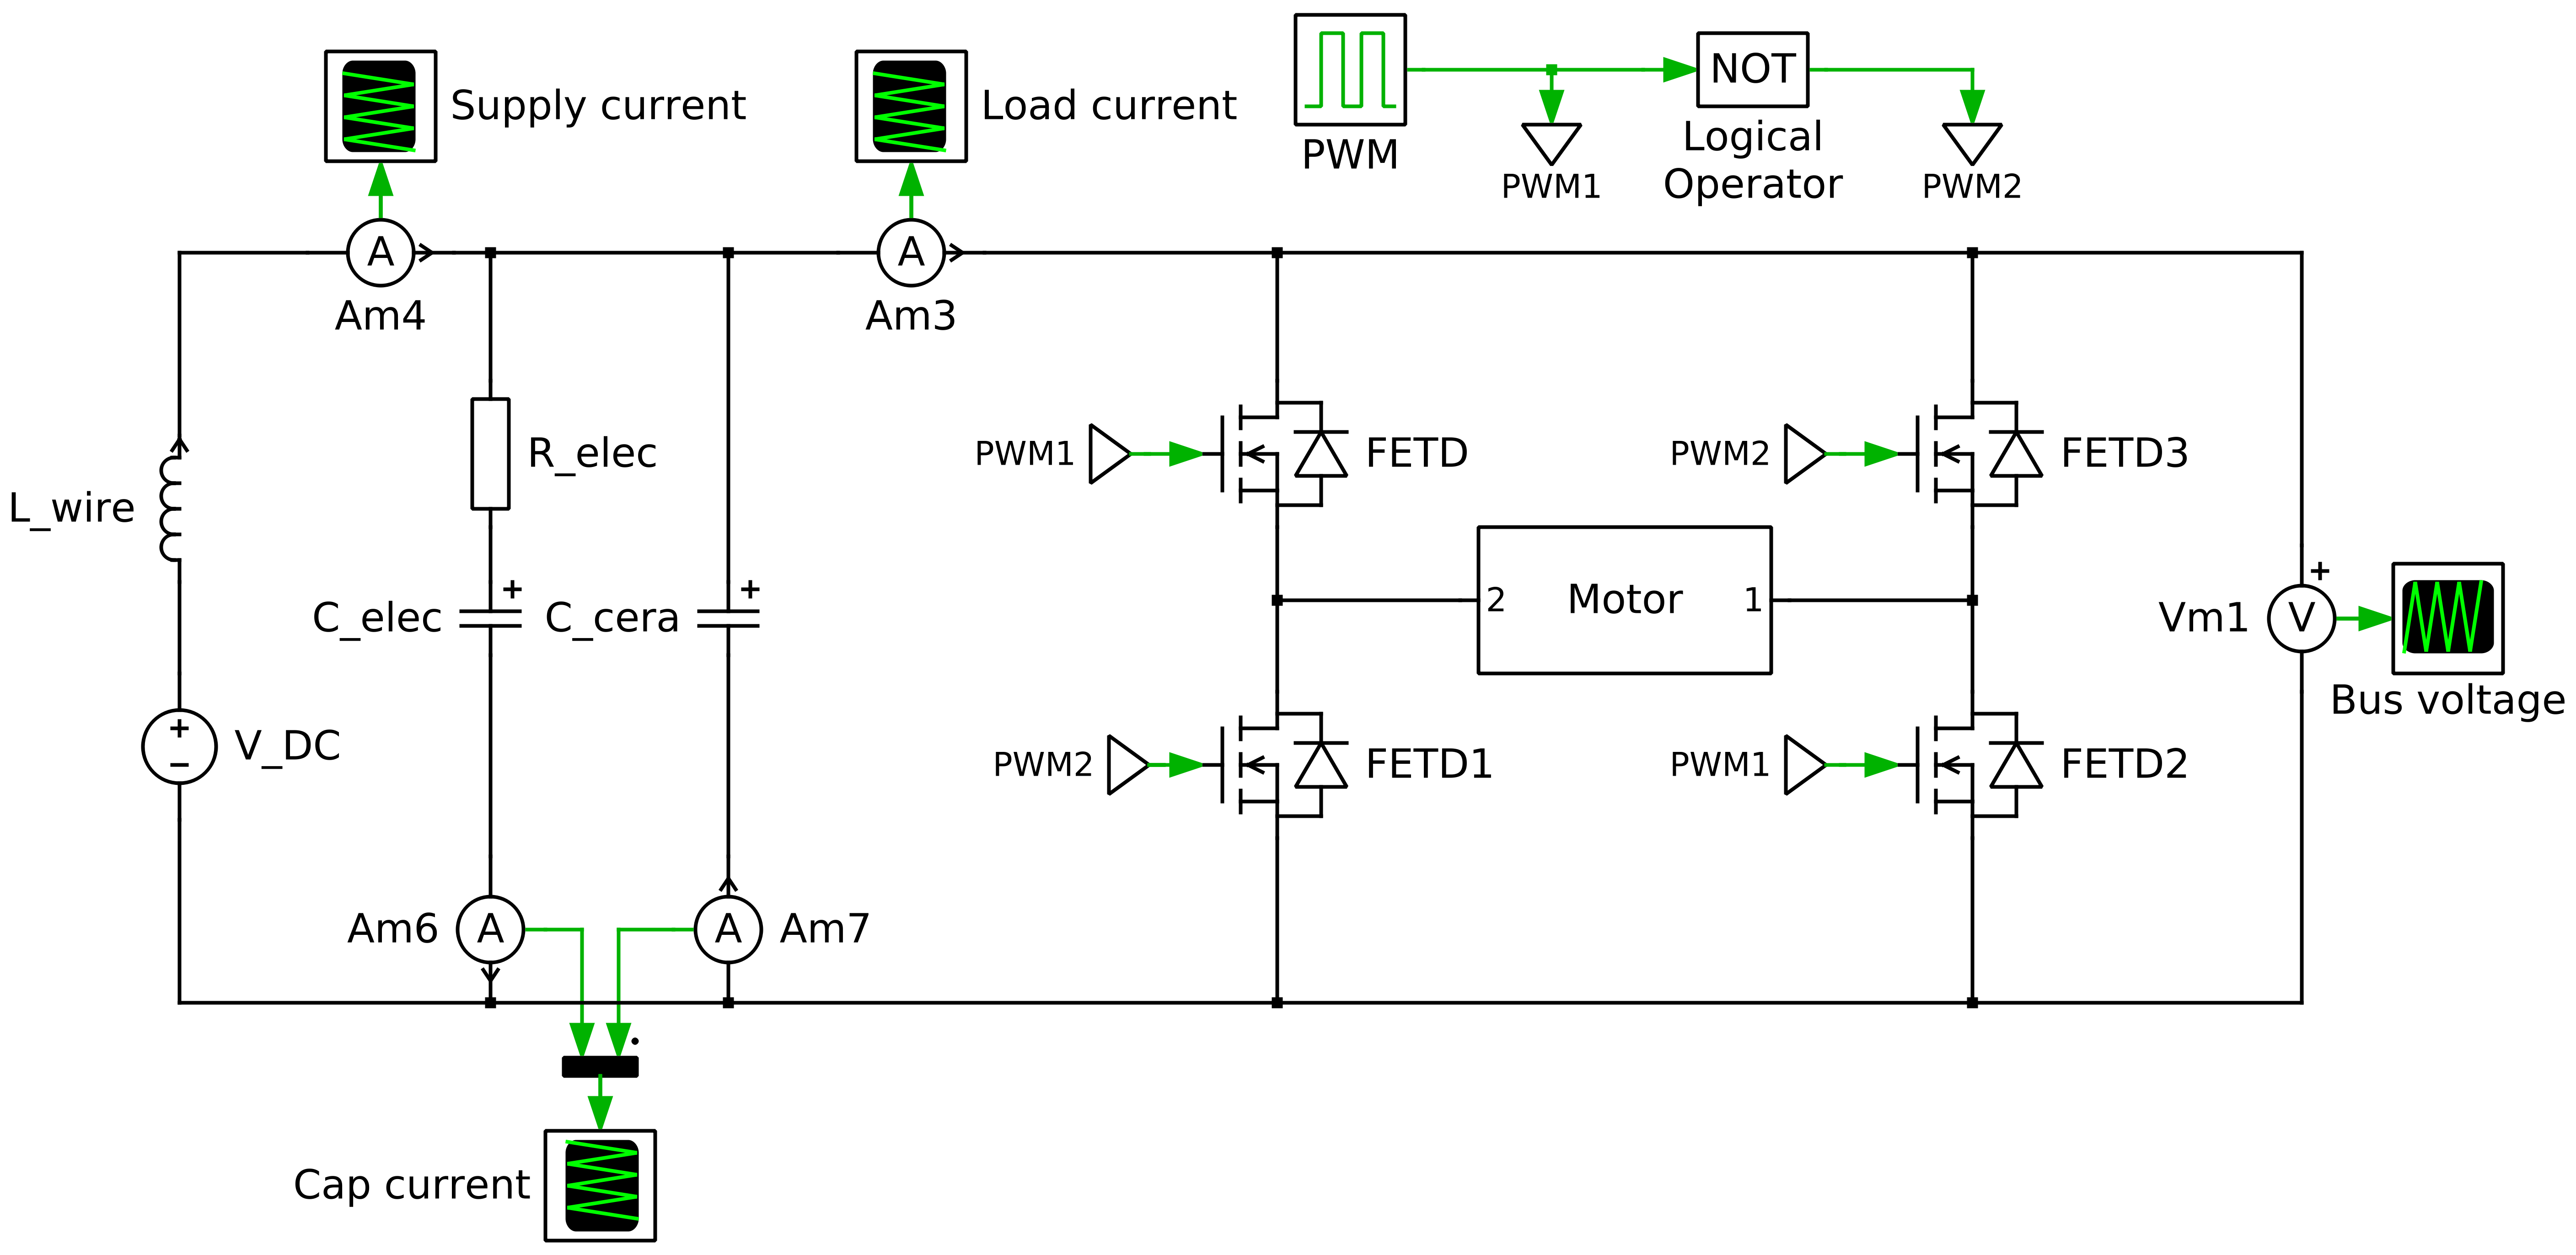
\includegraphics[width=1\linewidth]{graphics/plecs_schem.png}
	\caption[Full bridge circuit modelled in PLECS.]{Full bridge circuit with supply capacitors and wire inductance modelled using PLECS. The Motor box consists of an inductor and a resistor in series. All components apart from the MOSFETS have the same values as the chosen components.}
	\label{fig:plecs_schem}
\end{figure}	

Simulating the system at 50\% duty cycle yields a voltage ripple of approximately 24mV, which is definitely acceptable. 

It can also be noted that an effect of the inductance in the supply wires and the supply capacitors is that the supply current is low pass filtered and is thereby protected against the ripple current and only needs to supply the DC component of the load current.

The current drawn from the capacitors is shown in figure \ref{fig:cap_currents}.
Here it can be seen that the electrolytic capacitors supply the majority of the current, while the ceramic capacitors supply a small spike with high frequency content.
It should be noted that in the simulations there are no difference between the two types of capacitors other than the ESR put in series with the electrolytic capacitors. 

\begin{figure}[h]
	\centering
	%% This file was created by matlab2tikz.
%
%The latest updates can be retrieved from
%  http://www.mathworks.com/matlabcentral/fileexchange/22022-matlab2tikz-matlab2tikz
%where you can also make suggestions and rate matlab2tikz.
%
\definecolor{mycolor1}{rgb}{0.00000,0.44700,0.74100}%
\definecolor{mycolor2}{rgb}{0.85000,0.32500,0.09800}%


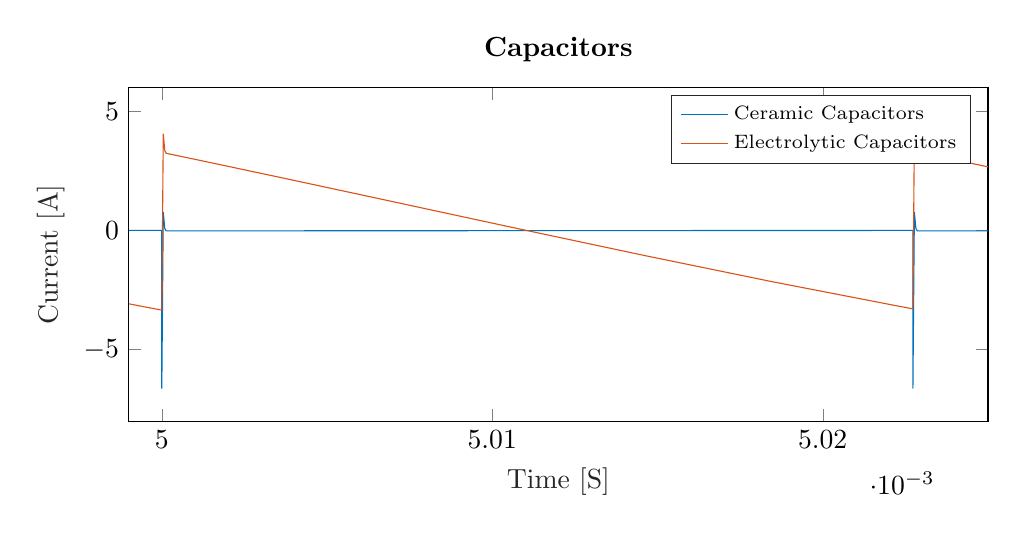
\begin{tikzpicture}




% \begin{axis}[%
% width=0.9\textwidth,
% height=1.2in,
% at={(0.758in,0.481in)},
% scale only axis,
% xmin=0.004999,
% xmax=0.005025,
% ymin=-5,
% ymax=5,
% ylabel style={font=\color{white!15!black}},
% ylabel={Current [A]},
% axis background/.style={fill=white},
% title style={font=\bfseries},
% title={Capacitors}
% legend style={legend cell align=left, align=left, draw=white!15!black}
% ]
% \addplot [color=mycolor1, forget plot]
%   table[row sep=crcr]{%




\begin{axis}[%
width=0.9\textwidth,
height=1.666in,
at={(0.758in,0.481in)},
scale only axis,
xmin=0.004999,
xmax=0.005025,
xlabel style={font=\color{white!15!black}},
xlabel={Time [S]},
ymin=-8,
ymax=6,
ylabel style={font=\color{white!15!black}},
ylabel={Current [A]},
axis background/.style={fill=white},
title style={font=\bfseries},
title={Capacitors},
legend style={legend cell align=left,font=\scriptsize , align=left, draw=white!15!black},
xtick={0.005,0.00501,0.00502}
]
\addplot [color=mycolor1]
  table[row sep=crcr]{%
0.0049010553385478	0.00342081159357233\\
0.00490489969343557	0.00683073660071676\\
0.00490874404832335	0.00991586664893029\\
0.00490909090909091	0.0101813275882865\\
0.00490909090909096	-6.63767713218716\\
0.00490913588166394	0.788632374646575\\
0.00490918085423691	0.0968134753000998\\
0.00490922582680989	-0.00983381196978428\\
0.00490967555253963	-0.0103095252998444\\
0.00491012527826937	-0.00895793028321945\\
0.00491057500399912	-0.00854569634641233\\
0.00491289980626855	-0.00643281216252056\\
0.00491522460853797	-0.00430374385953325\\
0.0049175494108074	-0.00216099641818635\\
0.00491987421307683	-2.65978258807836e-05\\
0.00492369979428432	0.00343331586571138\\
0.00492752537549182	0.00677023045901803\\
0.00493135095669931	0.00991965839131126\\
0.00493181818181813	0.0102885418851053\\
0.00493181818181818	-6.63795684124184\\
0.00493186309122796	0.788140209141018\\
0.00493190800063774	0.0970706595422914\\
0.00493195291004752	-0.00968459620855366\\
0.00493240200414533	-0.010151400317405\\
0.00493285109824314	-0.00922767791311507\\
0.00493330019234094	-0.00882378071900325\\
0.0049356105215896	-0.00627608882527975\\
0.00493792085083825	-0.00434505362802873\\
0.0049402311800869	-0.00213437587624032\\
0.00494254150933555	9.53670359069014e-05\\
0.00494636627166787	0.00360061858537619\\
0.00495019103400018	0.00703901460715084\\
0.00495401579633249	0.010148792099768\\
0.0049545454545454	0.0105586699059725\\
0.00495454545454545	-6.63771853889246\\
0.00495459015032096	0.786557805328613\\
0.00495463484609647	0.0976643538023345\\
0.00495467954187197	-0.00940476091145603\\
0.00495512649962704	-0.00993978708059062\\
0.0049555734573821	-0.00857857317189525\\
0.00495602041513717	-0.00816591337095129\\
0.0049583151501913	-0.00606782639068015\\
0.00496060988524543	-0.00395664904486392\\
0.00496290462029956	-0.00183438425385551\\
0.0049651993553537	0.00027740842506091\\
0.00496903087325131	0.00374628813147904\\
0.00497286239114892	0.00708566190254611\\
0.00497669390904653	0.0102308430991807\\
0.00497727272727267	0.010685341679721\\
0.00497727272727273	-6.63729580218999\\
0.00497731727074615	0.785182739111092\\
0.00497736181421957	0.0980802659485565\\
0.00497740635769299	-0.00922134889014892\\
0.0049778517924272	-0.00977371834118745\\
0.00497829722716142	-0.00883738412134694\\
0.00497874266189563	-0.00843919794694292\\
0.00498104199845287	-0.0059238355507687\\
0.0049833413350101	-0.0040186307720349\\
0.00498564067156733	-0.00183902675090497\\
0.00498794000812456	0.00035710955229637\\
0.00499179190075393	0.00384424013741791\\
0.00499564379338329	0.00726181015807148\\
0.00499949568601265	0.0103403911775377\\
0.00499999999999995	0.0107233299318876\\
0.005	-6.63678775329545\\
0.00500004447673189	0.784627777892562\\
0.00500008895346378	0.0981859652113108\\
0.00500013343019567	-0.0092018609164648\\
0.00500057819751456	-0.00979321463432026\\
0.00500102296483345	-0.00843310502509143\\
0.00500146773215235	-0.0080287074120009\\
0.00500377677864032	-0.00595109945391359\\
0.00500608582512829	-0.00386106136327458\\
0.00500839487161626	-0.00176029297984437\\
0.00501070391810423	0.000329411198857071\\
0.00501456587568511	0.00376585486603842\\
0.005018427833266	0.00707056768878767\\
0.00502228979084688	0.0101785379664605\\
0.00502272727272722	0.0105155195053972\\
0.00502272727272727	-6.63669528791197\\
0.0050227718773715	0.785481592291763\\
0.00502281648201573	0.0977955867894744\\
0.00502286108665995	-0.00940190195881785\\
0.00502330713310222	-0.00994616280641969\\
0.0050237531795445	-0.0090183414585101\\
0.00502419922598677	-0.00862558037378225\\
0.00502652935434658	-0.00611138202407391\\
0.00502885948270639	-0.00420805247858547\\
0.00503118961106621	-0.00202587201529669\\
0.00503351973942602	0.000174128206785015\\
0.00503738617751066	0.00363343469538768\\
0.0050412526155953	0.00702605089997999\\
0.00504511905367994	0.0100849998671229\\
0.00504545454545449	0.0103377257538093\\
0.00504545454545455	-6.63688438661501\\
0.0050454993184082	0.786909187571736\\
0.00504554409136186	0.0972936761155228\\
0.00504558886431551	-0.00964315408372496\\
0.00504603659385206	-0.0101688457131655\\
0.00504648432338861	-0.00881788004933393\\
0.00504693205292516	-0.00841271897506735\\
0.00504926853902644	-0.00631767727470978\\
0.00505160502512771	-0.00420712214877206\\
0.00505394151122899	-0.00208328771191457\\
0.00505627799733027	3.16047505261319e-05\\
0.00506012977709005	0.00346430797427311\\
0.00506398155684983	0.00677190482403178\\
0.00506783333660961	0.00988961814531208\\
0.00506818181818182	0.0101602465480153\\
0.00506818181818187	-6.63741638603617\\
0.00506822676429271	0.788263580426767\\
0.00506827171040355	0.0968710712364902\\
0.00506831665651439	-0.00981902461640649\\
0.00506876611762276	-0.010282819291199\\
0.00506921557873114	-0.00936583982423489\\
0.00506966503983952	-0.00896684900611833\\
0.00507200148913105	-0.0064211155171674\\
0.00507433793842259	-0.00449234590706937\\
0.00507667438771412	-0.00228026062001985\\
0.00507901083700566	-4.80677227454873e-05\\
0.00508284935926558	0.00343339431982481\\
0.0050866878815255	0.00685027548203943\\
0.00509052640378541	0.00994250061265101\\
0.00509090909090903	0.0102364341410595\\
0.00509090909090909	-6.63776191682534\\
0.00509095403119463	0.788414109103359\\
0.00509099897148016	0.0969253130139869\\
0.0050910439117657	-0.00977244042416769\\
0.00509149331462106	-0.0102542947538771\\
0.00509194271747643	-0.00890084705757577\\
0.00509239212033179	-0.00848784329587371\\
0.00509471010980675	-0.00637605440348255\\
0.00509702809928171	-0.00424860473551991\\
0.00509934608875667	-0.00210792975909035\\
};
\addlegendentry{Ceramic Capacitors}

\addplot [color=mycolor2]
  table[row sep=crcr]{%
0.0049010553385478	-0.915441839395498\\
0.00490489969343557	-2.02008944546105\\
0.00490874404832335	-3.06653627370542\\
0.00490909090909091	-3.15739364309411\\
0.00490909090909096	-3.15739364310866\\
0.00490913588166394	4.25578284216317\\
0.00490918085423691	3.55080766909668\\
0.00490922582680989	3.43099895230262\\
0.00490967555253963	3.29838689831377\\
0.00491012527826937	3.16703515437985\\
0.00491057500399912	3.03420023729996\\
0.00491289980626855	2.34110017146304\\
0.00491522460853797	1.63927639574104\\
0.0049175494108074	0.933249601497664\\
0.00491987421307683	0.227906177082332\\
0.00492369979428432	-0.918846892447618\\
0.00492752537549182	-2.02908008624217\\
0.00493135095669931	-3.08132645441947\\
0.00493181818181813	-3.20489120793354\\
0.00493181818181818	-3.20489120795537\\
0.00493186309122796	4.20799214847648\\
0.00493190800063774	3.50368169709691\\
0.00493195291004752	3.38368428511603\\
0.00493240200414533	3.25028965549427\\
0.00493285109824314	3.11773356924823\\
0.00493330019234094	2.98412907695456\\
0.0049356105215896	2.29115388523496\\
0.00493792085083825	1.58928909779206\\
0.0049402311800869	0.883900081273168\\
0.00494254150933555	0.179570804524701\\
0.00494636627166787	-0.971891453904391\\
0.00495019103400018	-2.08573965222604\\
0.00495401579633249	-3.14064893346222\\
0.0049545454545454	-3.28094792045158\\
0.00495454545454545	-3.28094792046613\\
0.00495459015032096	4.13016844417143\\
0.00495463484609647	3.428092171358\\
0.00495467954187197	3.30783548072941\\
0.00495512649962704	3.17493758595083\\
0.0049555734573821	3.04340834878531\\
0.00495602041513717	2.91042651790485\\
0.0049583151501913	2.22189270484523\\
0.00496060988524543	1.52567994879792\\
0.00496290462029956	0.826164624122612\\
0.0049651993553537	0.128065020835493\\
0.00496903087325131	-1.02202936300455\\
0.00497286239114892	-2.13347001265356\\
0.00497669390904653	-3.18471575261356\\
0.00497727272727267	-3.33703611806413\\
0.00497727272727273	-3.33703611808596\\
0.00497731727074615	4.07241109502502\\
0.00497736181421957	3.37225057452451\\
0.00497740635769299	3.25189005607535\\
0.0049778517924272	3.12027986907924\\
0.00497829722716142	2.98964814872306\\
0.00497874266189563	2.85799117581337\\
0.00498104199845287	2.17324157982512\\
0.0049833413350101	1.48047983761353\\
0.00498564067156733	0.784966991952388\\
0.00498794000812456	0.0911780343958526\\
0.00499179190075393	-1.05497919144545\\
0.00499564379338329	-2.16139660487534\\
0.00499949568601265	-3.2066133479675\\
0.00499999999999995	-3.33785721532331\\
0.005	-3.33785721535969\\
0.00500004447673189	4.07066818338353\\
0.00500008895346378	3.37131360285275\\
0.00500013343019567	3.2510084467649\\
0.00500057819751456	3.12077301707905\\
0.00500102296483345	2.99197915805416\\
0.00500146773215235	2.86174255228252\\
0.00500377677864032	2.17991762101883\\
0.00500608582512829	1.4905762026101\\
0.00500839487161626	0.798109154726262\\
0.00501070391810423	0.107245801111276\\
0.00501456587568511	-1.03223003423773\\
0.005018427833266	-2.13230920494243\\
0.00502228979084688	-3.17133878411551\\
0.00502272727272722	-3.28429267257161\\
0.00502272727272727	-3.28429267257161\\
0.0050227718773715	4.12503893459507\\
0.00502281648201573	3.42448077159497\\
0.00502286108665995	3.30441011337098\\
0.00502330713310222	3.17465105328301\\
0.0050237531795445	3.04583722598909\\
0.00502419922598677	2.91598394387256\\
0.00502652935434658	2.23211154308228\\
0.00502885948270639	1.53958590082766\\
0.00503118961106621	0.843786765552068\\
0.00503351973942602	0.149314537120517\\
0.00503738617751066	-0.987793491374759\\
0.0050412526155953	-2.08624917075213\\
0.00504511905367994	-3.1245759032754\\
0.00504545454545449	-3.21116772740061\\
0.00504545454545455	-3.21116772741516\\
0.0050454993184082	4.19972304494149\\
0.00504554409136186	3.49718167772517\\
0.00504558886431551	3.37731402221107\\
0.00504603659385206	3.24697386535991\\
0.00504648432338861	3.11796059356857\\
0.00504693205292516	2.98747435640689\\
0.00504926853902644	2.30020861748926\\
0.00505160502512771	1.60439322426828\\
0.00505394151122899	0.904558726528194\\
0.00505627799733027	0.205597670232237\\
0.00506012977709005	-0.932263559894636\\
0.00506398155684983	-2.03290280140209\\
0.00506783333660961	-3.07475351853645\\
0.00506818181818182	-3.16541938849696\\
0.00506818181818187	-3.16541938851151\\
0.00506822676429271	4.24721468395001\\
0.00506827171040355	3.54274894992705\\
0.00506831665651439	3.42298425603076\\
0.00506876611762276	3.29125734094123\\
0.00506921557873114	3.1603465270382\\
0.00506966503983952	3.02837585099041\\
0.00507200148913105	2.33636816850048\\
0.00507433793842259	1.63493908630335\\
0.00507667438771412	0.929554722511966\\
0.00507901083700566	0.224905788723845\\
0.00508284935926558	-0.918844584048202\\
0.0050866878815255	-2.02579574252013\\
0.00509052640378541	-3.07459532834037\\
0.00509090909090903	-3.17518959014706\\
0.00509090909090909	-3.17518959015433\\
0.00509095403119463	4.23782588414906\\
0.00509099897148016	3.5331533421122\\
0.0050910439117657	3.41326674421725\\
0.00509149331462106	3.28037942616356\\
0.00509194271747643	3.14876614561945\\
0.00509239212033179	3.0156744667911\\
0.00509471010980675	2.32288135642739\\
0.00509702809928171	1.62154641278175\\
0.00509934608875667	0.916161728986481\\
};
\addlegendentry{Electrolytic Capacitors}

\end{axis}
\end{tikzpicture}%
	\caption[Capacitor current simulation in PLECS.]{Current drawn from the electrolytic and ceramic capacitors, when simulating in PLECS. }
	\label{fig:cap_currents}
\end{figure}

\subsubsection{Relay Circuitry} % (fold)
\label{ssub:relay_circuitry}
Two relays are necessary for the system, the main relay and an inrush relay.
The main relay should be able to carry and break the total stall current, 80A.
This requirement is met by the LEV100A4ANG \cite{lev100}.
It is capable of carrying up to 100A continuous current and can break significantly more.
It has a 12V coil which requires $\approx$0.5A to hold in the closed state.
As mentioned previously the inrush relay is necessary to facilitate the initial charging of the supply capacitors.
The current to the capacitors is limited only by their ESR and a resistor should be added to limit this inrush current.
Adding the resistor to the main current path would introduce considerable losses and limit the performance of the system.
The inrush relay is implemented in parallel with the main relay to supply a temporary alternate current path in which the resistor is placed.
The size of the resistor is somewhat irrelevant so long as it is large enough to protect the circuitry.
Having a larger resistance will only increase the time it takes before the capacitors are sufficiently charged.
For this reason a 180$\Omega$ 5W resistor is used.
As shown by equation \ref{eq:cap_boot_time}, the charging time can be found as 

\begin{equation}
	T_{charge} = 5\cdot R_{inrush}\cdot C_{supply} = 5\cdot 180\cdot 1320\cdot10^{-6} = 1.188 \text{[S]}
\end{equation}

Therefore, on bootup, the system will not be able to start running the motors until $\approx$1.2 S have passed.
This is estimated to be sufficient as this is well below the boot time of the remaining system.
The relay chosen for this application is the G6B-1114P \cite{g6b} with a 12V coil.
Being a significantly smaller relay, carrying up to 5A, the G6B-1114P requires only 16.7mA to hold in the closed state.\\~\\
Figure \ref{fig:relaycircuit} shows the driving circuitry for the inrush relay. 
The circuitry is identical for the main relay but can be seen in the full schematic in appendix \ref{app:controller_board_schem}.
As can be seen, the relay can be switched on and off by a signal to the MOSFET Q18.
This signal is high only when signals \texttt{INRUSH} and \texttt{EM\_DIS} are high.
\texttt{EM\_DIS} is the signal from the safety circuitry and \texttt{INRUSH} allows the user to toggle the relay.
Designing the circuit in this manner ensures that the motor will remain disengaged in case of an activated safety condition.
Finally, A flyback diode is placed in parallel with the inductor in the relay to create an alternate current path when the MOSFET is switched off.

\begin{figure}[H]
	\centering
	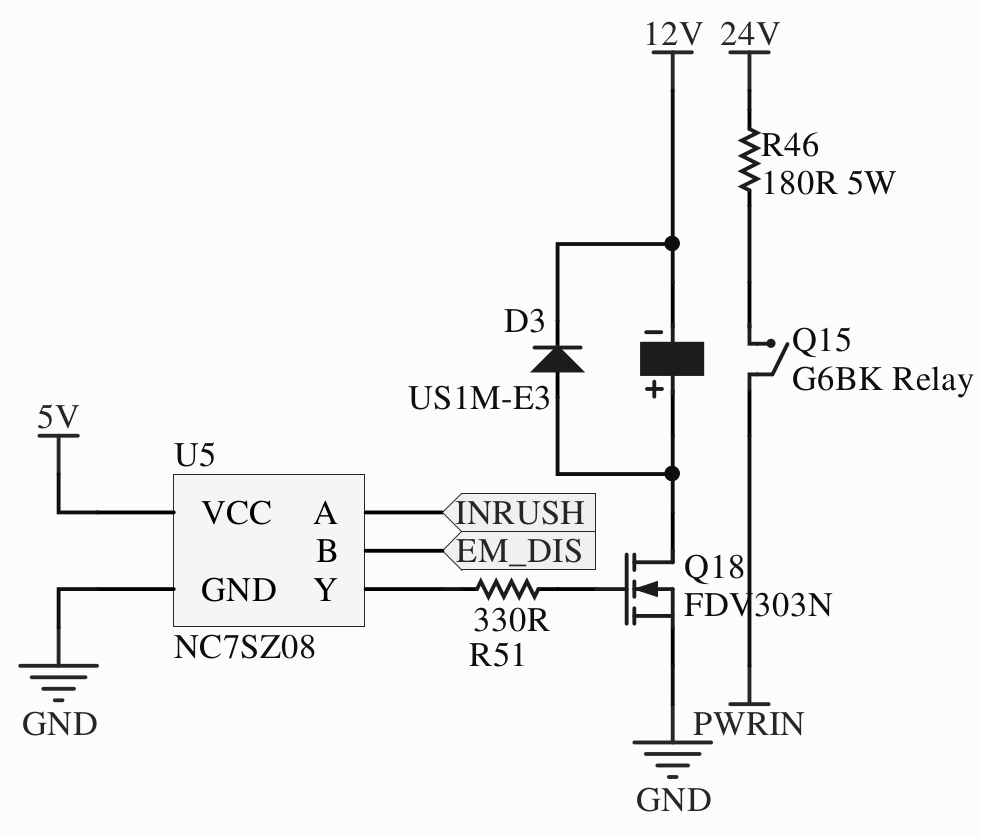
\includegraphics[width=.5\linewidth]{graphics/relay_circuit}
	\caption{Circuitry related to the inrush relay.}
	\label{fig:relaycircuit}
\end{figure}
% subsubsection relay_circuitry (end)


\subsubsection{Motor Current Sensing}
Measuring current in an H-Bridge with a shunt resistor can be done in a number of ways.
The shunt resistor can be placed in various positions in the H-bridge.
The three main ones are high-side, in-line and low-side placement of the shunt resistor.
\cite{shunt_placement} and \cite{Current_Sense_Circuit_Collection} specifies the advantages and disadvantages of the three configurations.
\mikkel{add a quick summary of each and highlight the selected one?} 
It was decided to use the low-side configuration as it has low common voltage, it only needs a single sided supply and because bi-directional current measurement is not needed in this application.

\paragraph{Requirements for the Current Measuring Circuit} ~\\% (fold)
\label{par:requirements_for_the_current_measuring_circuit}

The output of the current measuring circuit is an analogue signal that is measured by the ADC of the Zynq chip.
According to the Zynq ADC user guide \cite{zynq_adc}, the measurable input range is from 0V to 1V, but the maximum allowed input voltage is 1.9V according to \cite{adc_zynq_webanswer}.
The absolute maximum current through the motor is the stall current which is 80A, but the motor will run well below this level in normal operation.
The nominal current of the motor is 6A but allowing for some headroom maximum current spikes during normal operation are not expected to exceed 30A. 
It was therefore decided that the circuit  needs to be able to measure currents of at least up to 40A.
The resolution per ampere is increased by decreasing the current range that can be measured.
If the current gets any higher the ADC input should not be harmed meaning that the input voltage should not exceed 1.9V.

\paragraph{Designing the Current Measuring Circuit} ~\\% (fold)
\label{par:designing_the_current_measuring_circuit}

Placing a shunt resistor in the low-side configuration raises the voltage potential of the low-side of the H-bridge.
This may influence the gate signal required to open the MOSFETs of the H-bridge.
In addition, the shunt resistor will, regardless of placement result in a powerloss proportional to its size.
For these reasons minimizing the value of the shunt resistor is important. 
The smallest value available from the electronics supplier used at SDU provides a 200$\mu\Omega$ SMD shunt resistor.
Such a small resistance yields a minimal voltage drop and thus keeps power consumption at a minimum.\\
The resulting voltage from the motor stalling, that is an 80A current flowing through the resistor would result in only a 16mV voltage drop.
Since the input range of the ADC is 0-1V, this low voltage would yield very poor resolution in the area of actual interest, 0-40A.
An amplifier circuit is necessary.
Purpose built current-sense amplifiers exist which are used specifically for amplifying the voltage drop across a shunt resistor.
One such amplifier is the \texttt{INA286AID} from Texas Instruments \cite{INA286AID}.
It has a gain of 100, lifting the voltage resulting from motor stall to 1.6V as seen from equations \ref{eq:adc_input_voltage1} and \ref{eq:adc_input_voltage2}.
\begin{equation}
	V_{max,input} = G \cdot V_{shunt}
	\label{eq:adc_input_voltage1}
\end{equation}
\begin{equation}
	V_{max,input} = G \cdot R_{shunt} \cdot I_{stall} = 100 \cdot 200\cdot10^{-6} \cdot 80 = 1.6V
	\label{eq:adc_input_voltage2}
\end{equation}
The measurable range using this IC is 0-50A as seen from \ref{eq:adc_input_voltage3}.

\begin{equation}
	I_{max, measurable} = \frac{V_{max, measurable}}{R_{shunt}\cdot G} = \frac{1}{100 \cdot 200\cdot10^{-6} } = 50A
	\label{eq:adc_input_voltage3}
\end{equation}

It has a very low offset allowing it to be used in applications where the voltage drop across the shunt resistor is only a few mV.
\\
Using this configuraion the resolution can be calculated as:
\begin{equation}
	Res_{amp} = \frac{I_{max,measurable}}{Res_{ADC}} = \frac{50}{2^{12}}  = 12.2 mA
\end{equation}
Where $Res_{amp}$ is the resolution in amperes and $Res_{ADC}$ is the resolution of the ADC on the Zynq.
\\~\\
This design meets the required design specifications and the schematics can be seen in figure \ref{fig:currentmeasure}.
As can be seen, the \texttt{INA286} in this configuration requires only the voltage input, \texttt{POWER\_SHUNT+/-} from the schematic on figure \ref{sfig:hbridgeshunt}, to generate a suitable output which is then fed directly to the ADC through the anti-aliasing filter shown on figure \ref{sfig:ina286aidschematic}.

\begin{figure}
	\centering
	\begin{subfigure}[b]{0.49\textwidth}
		\centering
		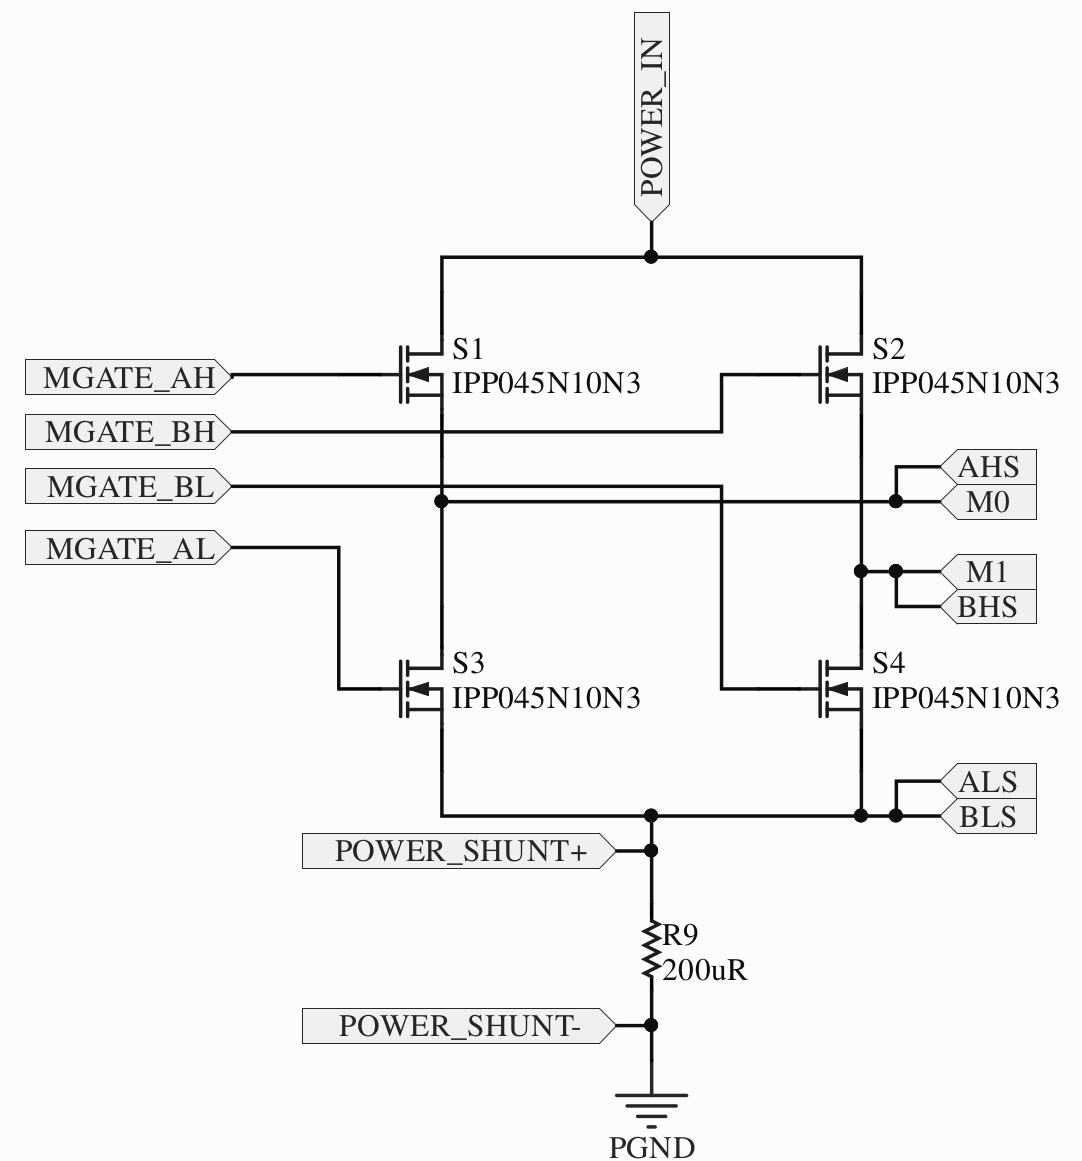
\includegraphics[width=\linewidth]{graphics/hbridge}
		\caption{H-bridge with shunt resistor in low-side configuration.}
		\label{sfig:hbridgeshunt}	
	\end{subfigure}
	\begin{subfigure}[b]{0.49\textwidth}
		\centering
		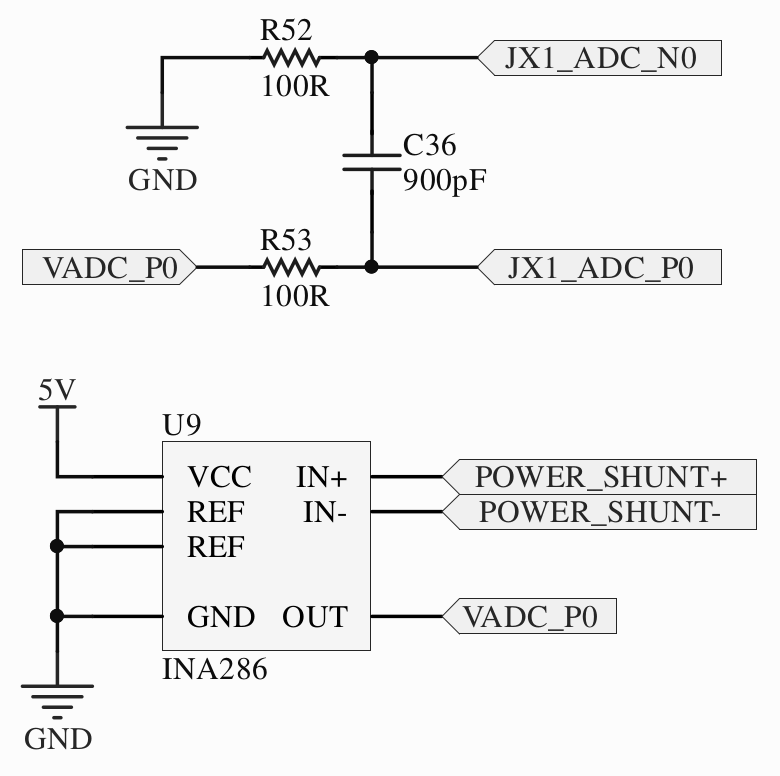
\includegraphics[width=\linewidth]{graphics/ina286}
		\caption{Schematic of the INA286AID as used in the project.}
		\label{sfig:ina286aidschematic}
	\end{subfigure}
	\caption{Schematics relating to the current measurement circuitry.}
	\label{fig:currentmeasure}
\end{figure}

% subsubsection designing_the_current_measuring_circuit (end)



% subsection relay_circuitry (end)

\subsubsection{Endstop Detection} % (fold)
\label{ssub:endstop_detection}
As described in section \ref{subsub:safety} it was decided to use infrared transceivers to detect endstops.
It was decided to use the \texttt{TCST2103} \cite{tcst2103} as it has the wanted functionality.
It contains an infrared emitter pointing at a photo transistor, that conducts current proportional to the infrared light received.
In this project it will be used to detect if the infrared light is blocked by the cart or not. 
The circuit shown in figure \ref{fig:tcst_circuit} was realised to convert the current conducted to a voltage level. 
The output is fed to a schmitt trigger circuit in order to be able to use the result as a boolean reference.
The schmitt-trigger circuit is designed to have a high threshold of 3V and a low threshold of 1V.
The circuit can be seen in appendix \ref{app:controller_board_schem}.

\subsubsection{Voltage Rails} % (fold)
\label{subsub:voltage_rails}
In the design of the board it is necessary to determine which voltage rails are required for the system to function.
The power delivery for the MicroZed was designed by the authors in an earlier project \cite{isaswarm} and will be reused with minor changes.
This power delivery system provides, amongst other voltages, the 3.3V rail, originally intended for powering the MicroZed IO banks only.
In this system however, the RF tranceiver is also powered from this rail.
As a result a review of the circuitry around the 3.3V rail is necessary to ensure that it can provide the required power.
The MicroZed power delivery system, the encoders of the system, the endstops and part of the emergency circuitry are all driven from a 5V rail.
The Motor Driver, the HIP4081 \cite{driver} and the relay driving circuitry is driven from a 12V rail.
Finally, the motor is driven from a 24V rail, which will also be the main supply for the system.
This rail is not crucial to the design of the board as it is provided by an external, mains connected power supply and will not be explored further in this section.\\
The current requirement for each of these rails are discussed in the following paragraphs

\paragraph{3.3V:} % (fold)
\label{par:3_3v}
As mentioned, this rail is intended for powering the MicroZed IO banks.
In the original design the \texttt{LMR10510XMF} DC/DC converter is used to provide the necessary power.
This chip is capable of supplying up to 1A.
Components exist in the same series which are pin compatible and are capable of supplying up to 2A.
The RF Transceiver used in this project, however, requires only up to 15mA when receiving data and is considered unnecessary to upgrade the current capacity of the rail.
% paragraph 3_3v_ (end)

\paragraph{5V:} % (fold)
\label{par:5v}
This rail supplies, mainly, the MicroZed.
The maximum expected current draw from the microzed is 1.85A at 5V \cite{microzed}.
This includes the current drawn from the 3.3V rail.
In addition, in this design, the 5V rail also powers the encoders, endstops and emergency circuitry.
The \texttt{HEDS-5540} \cite{heds5540} encoder requires a maximum of 85mA.
The endstops are realised using the \texttt{TCST2103} infrared sensor \cite{tcst2103}.
The majority of the current supplied to this sensor is used to power the infrared LED present in the component.
This current is decided by the resistor put in series with the LED and is estimated to be around 50mA per LED for a total of 100mA.
Another 10mA is added to that figure due to the collector current possible on the transistor side.\\
Finally the emergency circuitry along with some other digital electronics are powered from the 5V rail.
As these are all digital IC's that operate on nothing but signals, their individual powers are negligible but a very conservative 25mA power budget is provided for all of the digital electronics on the 5V rail. This brings the total power budget for the 5V rail to $\approx$2.1A.
See table \ref{tab:5vpowerbudget} for a full overview.

\begin{table}
	\centering
	\begin{tabular}{l|r}
		 Component & Current [mA]\\
		 \hline
		 MicroZed & 1850\\
		 HEDS-5540 & 85\\
		 TCST2103 & 110\\
		 Digital & 25\\
		 \hline
		 Total & 2070
	\end{tabular}
	\caption{Power budget for the 5V rail}
	\label{tab:5vpowerbudget}
\end{table}

In \cite{isaswarm} the authors used a design in which the \texttt{PTH08080} is used to generate a 5V rail.
Reusing this module will save on design time as well as the budget available to the project and as such is desirable.
This module can supply 2.25A at 5V and should therefore be sufficient for this application.
The \texttt{PTH08080} design will be reused for this project.
% paragraph 5 (end)

\paragraph{12V:} % (fold)
\label{par:12v}
This rail powers the \texttt{HIP4081} motor driver, the relay coils, the bootstrap circuitry and the 5V DC/DC converter.
The \texttt{PTH08080} DC/DC converter has a maximum input voltage of 18V and must be powered from the 12V rail rather than the 24V rail.
The module can provide 2A at 5V and as such will require $\approx$0.85A from the 12V rail, assuming 100\% efficiency.

There are two relays in the design, a smaller relay for controlling the inrush current and the larger main supply relay.
Both of these require power to stay in the closed position.
The first, the \texttt{G6B}, requires 16.7mA while the former, the \texttt{LEV100A4ANG}, requires 461mA.

The motor driver of the system, the HIP4081 requires only 10mA.
As mentioned, the bootstrap circuitry is also powered from the 12V rail.
Rather than a steady supply, this circuitry requires a large peak current for short periods while charging in between switching.
For this reason the design choice here is to determine what is available and choose the component which yields the most headroom while still being economically feasible.
Amongst all of the components the total power budget for the 12V rail is $\approx$1340mA.
See table \ref{tab:12vpowerbudget} for a full overview.

\begin{table}
	\centering
	\begin{tabular}{l|r}
		 Component & Current [mA]\\
		 \hline
		 PTH08080 & 850\\
		 G6B & 16.7\\
		 LEV100A4ANG & 461\\
		 HIP4081 & 10\\
		 \hline
		 Total & 1337.7
	\end{tabular}
	\caption{Power budget for the 12V rail}
	\label{tab:12vpowerbudget}
\end{table}

The PTN78020 delivers 6A at 12V and is part of the same series as the PTH08080 described earlier.
This allows many of the same design procedures to be reused.
In addition, the 6A current limit leaves sufficient room for the current spikes expected from the bootstrap circuitry.
% paragraph 12v_ (end)

% subsection voltage_rails (end) 


\subsubsection{12V Rail Circuitry}

\begin{figure}
	\centering
	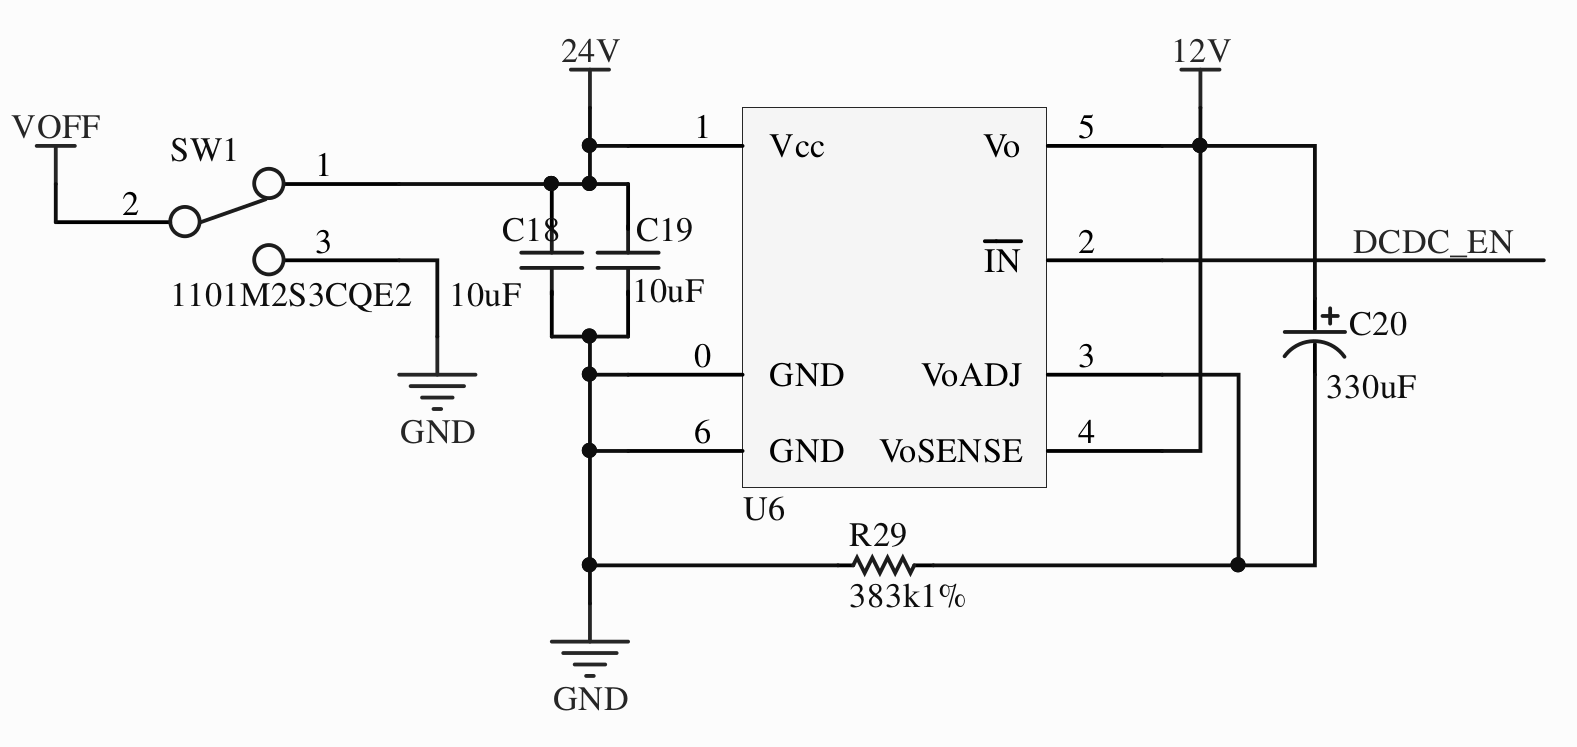
\includegraphics[width=\linewidth]{graphics/dcdc12v}
	\caption[PTN78020H DC/DC converter circuitry.]{The \texttt{PTN78020H} DC/DC converter and the appertaining circuitry.}
	\label{fig:dcdc12v}
\end{figure}

The \texttt{PTN78020H} DC/DC converter is used to generate the 12V rail. 
The component requires input and output capacitors in order to function properly and a resistor is needed to set the desired output voltage. 
The circuit used is based on the typical application circuit shown in the datasheet \cite{PTN78020H} and is implemented as shown in figure \ref{fig:dcdc12v}.
A resistor is required from \texttt{VoADJ} to ground to set the desired output voltage, in this case 12V.
To generate 12V a 383 k$\Omega$ resistor is needed.
\texttt{VoSENSE} should be connected close to the main load to allow for more precise regulation of the output.
This feature is mainly useful when the load is placed far from the supply and can be left floating if the accuracy of the rail is not important.
It was decided to simply short it to the 12V rail at the component since the load is placed relatively close to the supply.
$\overline{\text{\texttt{IN}}}$ carries the inhibit signal.
Pulling this low will disable the output of the component.
This is done by toggling the switch \texttt{SW1}. 
This will open a MOSFET which in turn will pull the \texttt{DCDC\_EN} signal low.
The datasheet also specifies that a ceramic capacitance of at least 18.8 $\mu$F is needed at the input. 
It was chosen to use two 10 $\mu$F capacitors.
In order to ensure stability the \texttt{PTN78020H} needs an output capacitance of 330 $\mu$F.
The datasheet specifies that if the application has load transients additional capacitance should be added to improve the response of the regulator.
While the load at the 12V rail is mostly steady, it does supply the bootstrap capacitors which create a slight ripple on the rail.
It was therefore decided to use two 330 $\mu$F electrolytic capacitors in parallel.
As suggested by the datasheet an additional 20 $\mu$F of ceramic capacitance is added to the output to further improve the transient response.\\

\subsubsection{5V, 3.3V and 2.5V Rail Circuitry} % (fold) 
\label{subsub:pth08080w}
As mentioned previously the choice of these component and the design of the circuitry around them was done by the authors in a previous project \cite{isaswarm} and the details of the design will be omitted for this discussion.
The \texttt{PTH08080W} and \texttt{LMR10510XMF} are responsible for creating the 5V and 3.3V rails, respectively and the 2.5V reference is created by the \texttt{TL431AIDBZT}.
% subsection pth08080w (end)
